% ============================================================
%  Agentic AI for Near-Real-Time Ocean Hazard Assessment
%  8th NOAA AI Workshop (2026) - uses neurips_2025.sty for formatting
%
%  COMPILATION INSTRUCTIONS
%  Requires neurips_2025.sty (included in paper/ directory).
%
%  Build (from paper/ directory):
%    cd paper
%    tectonic paper.tex
%
%  (tectonic resolves the bibliography and reruns automatically; a plain
%   TeX Live install can use: pdflatex, bibtex, pdflatex, pdflatex)
% ============================================================

\documentclass{article}

\usepackage[main, final]{neurips_2025}

% Override conference notice for NOAA AI Workshop
\makeatletter
\renewcommand{\@noticestring}{8th NOAA AI Workshop (2026).}
\makeatother

% Numbered citations [1], [2], ... per NeurIPS convention
\setcitestyle{numbers,square}

\usepackage[utf8]{inputenc}
\usepackage[T1]{fontenc}
\usepackage{hyperref}
\usepackage{xurl}
\usepackage{booktabs}
\usepackage{amsfonts}
\usepackage{amsmath}
\usepackage{amssymb}
\usepackage{nicefrac}
\usepackage{microtype}
\usepackage{xcolor}
\usepackage{graphicx}
\usepackage{subcaption}
\usepackage{placeins}
\usepackage{capt-of}
\usepackage{algorithm}
\usepackage{algorithmic}
\usepackage{enumitem}
\usepackage{orcidlink}
\usepackage{tikz}
\usetikzlibrary{shapes.geometric, arrows.meta, positioning, fit, backgrounds, calc}
\usepackage{listings}
\usepackage{tcolorbox}
\tcbuselibrary{listings,breakable,skins}

% ---- Prompt box styling: AI/ML research paper convention ----
% Color palette per model tier
\definecolor{promptfast}{HTML}{0D9488}       % teal-600
\definecolor{promptstandard}{HTML}{2563EB}   % blue-600
\definecolor{promptquality}{HTML}{7C3AED}    % violet-600
\definecolor{promptbg}{HTML}{F8FAFC}         % slate-50

% Header bar (takes color + title)
\newcommand{\promptlabel}[2][black!70]{%
  \begin{tcolorbox}[
    enhanced,
    arc=2.5pt,
    boxrule=0pt,
    colback=#1, colframe=#1,
    rounded corners=northwest, rounded corners=northeast,
    sharp corners=south,
    left=8pt, right=8pt, top=3pt, bottom=3pt,
    after skip=-0.6pt, before skip=10pt,
  ]
  \sffamily\small\bfseries\textcolor{white}{#2}
  \end{tcolorbox}%
}

% Content body (monospace listing)
\newtcblisting{promptbox}{
  listing only,
  enhanced,
  colback=promptbg,
  colframe=black!15,
  boxrule=0.4pt,
  arc=2.5pt,
  rounded corners=southwest, rounded corners=southeast,
  sharp corners=north,
  borderline west={2pt}{0pt}{black!12},
  left=8pt,
  right=7pt,
  top=6pt,
  bottom=6pt,
  listing options={
    basicstyle=\ttfamily\fontsize{7.5}{9.8}\selectfont,
    breaklines=true,
    breakatwhitespace=true,
    columns=fullflexible,
    keepspaces=true,
  },
  breakable,
  before skip=0pt,
  after skip=10pt,
}

% Agent trace colors
\definecolor{traceqc}{HTML}{059669}       % emerald-600
\definecolor{traceanomaly}{HTML}{D97706}  % amber-600
\definecolor{tracefsm}{HTML}{DC2626}      % red-600
\definecolor{tracescenario}{HTML}{2563EB} % blue-600
\definecolor{traceverify}{HTML}{7C3AED}   % violet-600
\definecolor{tracebg}{HTML}{FAFAF9}       % stone-50

% Agent trace label (colored left stripe + agent name tag)
\newcommand{\tracelabel}[2][black!60]{%
  \begin{tcolorbox}[
    enhanced,
    arc=2pt,
    boxrule=0pt,
    colback=#1, colframe=#1,
    rounded corners=northwest, rounded corners=northeast,
    sharp corners=south,
    left=8pt, right=8pt, top=2.5pt, bottom=2.5pt,
    after skip=-0.6pt, before skip=8pt,
  ]
  \sffamily\footnotesize\bfseries\textcolor{white}{#2}
  \end{tcolorbox}%
}

% Agent trace body (JSON output box)
\newtcblisting{tracebox}{
  listing only,
  enhanced,
  colback=tracebg,
  colframe=black!12,
  boxrule=0.3pt,
  arc=2pt,
  rounded corners=southwest, rounded corners=southeast,
  sharp corners=north,
  left=7pt,
  right=7pt,
  top=5pt,
  bottom=5pt,
  listing options={
    basicstyle=\ttfamily\fontsize{7}{9}\selectfont,
    breaklines=true,
    breakatwhitespace=true,
    columns=fullflexible,
    keepspaces=true,
  },
  breakable,
  before skip=0pt,
  after skip=8pt,
}

% Float placement: push float-only pages to top, allow more floats,
% and reduce penalties for text sharing a page with floats.
\makeatletter
\setlength{\@fptop}{0pt}
\renewcommand{\topfraction}{0.9}        % up to 90% of page for top floats
\renewcommand{\bottomfraction}{0.8}     % up to 80% for bottom floats
\renewcommand{\textfraction}{0.07}      % at least 7% text (allows dense float pages)
\setcounter{topnumber}{3}               % up to 3 floats at top
\setcounter{bottomnumber}{2}            % up to 2 floats at bottom
\setcounter{totalnumber}{5}             % up to 5 floats per page
\renewcommand{\floatpagefraction}{0.7}  % float page when >=70% floats
\makeatother

\hypersetup{
  colorlinks=true,
  linkcolor=blue!60!black,
  citecolor=blue!60!black,
  urlcolor=blue!60!black,
}

% ============================================================
%  Title
% ============================================================

\title{Agentic AI for Near-Real-Time Ocean Hazard Assessment}

% ============================================================
%  Authors
% ============================================================

\author{%
  Kevin Lee\orcidlink{0009-0004-0388-9260}$^{1,2}$\thanks{Corresponding author. Email: \texttt{kevinlee69720@g.ucla.edu}} \quad
  Alison J. March\orcidlink{0009-0000-3643-8061}$^{3}$ \\[4pt]
  $^1$NASA Jet Propulsion Laboratory, La Ca\~{n}ada Flintridge, CA, USA \\
  $^2$Department of Mechanical and Aerospace Engineering, UCLA, Los Angeles, CA, USA \\
  $^3$College of Engineering and Applied Science, University of Colorado, Boulder, CO, USA \\
}

\begin{document}

\maketitle

\footnotetext[1]{Source code: \url{https://github.com/magnaprog/Agentic-AI-for-Near-Real-Time-Ocean-Hazard-Assessment}}

% ============================================================
%  Abstract
% ============================================================

\begin{abstract}
Tsunami assessment requires duty scientists to interpret
heterogeneous sensor data within minutes of a seismic event.
While NOAA's operational warning systems provide authoritative
forecasts, situational awareness can be improved by automating
data integration and report generation without replacing
established workflows.
We present an agentic AI framework for near-real-time ocean
hazard assessment, demonstrated on seismogenic tsunami detection,
that ingests NOAA DART bottom-pressure records, CO-OPS
water-level observations, and USGS seismic event feeds through a
deterministic finite-state machine orchestrating quality control,
ensemble anomaly detection, NNLS-based scenario
inversion~\citep{lawson1974solving, percival2011extraction}, and a
nine-check verification stage.
Scenarios that fail verification trigger an ABSTAIN mechanism
suppressing probabilistic guidance and routing output to a
mandatory human review gate.
An optional LLM layer works under bounded autonomy, unable to
modify detection state or bypass verification.  It synthesizes
operator-readable narratives.  While an event is open, an
investigator chooses its own read-only queries over the recorded
evidence to answer questions the deterministic pipeline leaves open.
A database privilege boundary, not an instruction in a prompt, keeps
what it finds advisory.
Retrospective evaluation on five Pacific tsunamigenic earthquakes
($M_w$\,8.1--9.1, including T\={o}hoku 2011, Chile 2010,
Illapel 2015, Iquique 2014, and Samoa 2009) using archived DART
data shows that event-mode stations (high-cadence sampling) within
${\sim}3{,}000$\,km reach the anomaly detection threshold
($T_1{=}0.35$), with the nearest station reaching the escalation
tier ($T_3{=}0.85$) in three of the five events and a lower tier
in Iquique (ASSESS) and Samoa (INVESTIGATE);
standard-mode stations (15-min sampling) score at or near zero.
Those stations are filter-degraded by the Nyquist criterion, and all
but one are also too distant for either coseismic deformation or
tsunami arrival to fall inside the six-hour evaluation window, so this
evaluation does not separate the two effects.
The earliest detections (2.7\,min post-earthquake) correspond to
coseismic seafloor deformation, not the tsunami wave itself;
actual tsunami arrivals appear on longer timescales depending on
source--station distance.
The complete implementation is publicly available under a
noncommercial license.\footnotemark[1]
\end{abstract}

\noindent\textbf{Keywords:}
tsunami detection, agentic AI, ocean hazard assessment,
multi-agent system, finite-state machine, anomaly detection

% ============================================================
%  1. Introduction
% ============================================================

\section{Introduction}

Tsunamis rank among the most destructive geophysical hazards. The 2004
Indian Ocean event caused approximately 230,000
fatalities~\citep{synolakis2006tsunami}; the 2011
T\={o}hoku event caused 19,759 confirmed deaths with 2,553 persons still missing~\citep{npa2023tohoku}, and field surveys recorded
run-up heights exceeding 30\,m along the Sanriku coast~\citep{mori2011survey}. NOAA's operational warning
centers, the National Tsunami Warning Center (NTWC) and Pacific Tsunami
Warning Center (PTWC), provide authoritative forecasts using the
Deep-ocean Assessment and Reporting of Tsunamis (DART) buoy
network~\citep{bernard2011history} and the Short-term Inundation
Forecasting for Tsunamis (SIFT) system~\citep{titov2005realtime,
gica2008development}. These systems meet the rigorous validation
standards required for life-safety products and represent decades of
operational development.

Yet a gap in situational awareness persists. Duty
scientists who monitor real-time data streams must manually integrate
heterogeneous sensor feeds (deep-ocean bottom-pressure records, coastal
water-level gauges, and seismic event catalogs) while simultaneously
evaluating evolving scenarios and communicating uncertainty to colleagues
and decision-makers. Under the operational pressure of a developing
event, this manual integration is both time-consuming and error-prone.
During fast-developing events, duty scientists may have as few as
3--5 minutes between initial seismic detection and the need for a
preliminary assessment~\citep{bernard2015evolution}, while simultaneously monitoring dozens of
sensor streams across multiple visualization tools.

Agentic AI can address this gap by automating data integration. Recent
work on LLM-based agents~\citep{yao2023react, wang2024survey} has
shown the value of combining reasoning with tool use, though
LLM-driven approaches introduce non-determinism that is unacceptable
in safety-critical hazard assessment. An agentic framework that constrains LLM involvement to advisory
roles while using deterministic signal processing for detection and
assessment can automate data integration, anomaly detection, scenario
ranking, and structured communication in a pipeline that produces
human-interpretable probabilistic guidance. The challenge is
implementing such a framework with the safety properties required in a
maritime hazard context: no autonomous public communication, no
interference with operational data streams, deterministic reasoning that
can be audited after the fact, and a required Human Review Gate before
any guidance is distributed internally.

We present a \textbf{bounded agentic AI framework} that addresses these
requirements. The system ingests DART buoy observations, NOAA CO-OPS water-level
data, and USGS seismic event catalogs through the pipeline
(retrospective evaluation in this paper uses DART bottom-pressure
records; the CO-OPS and USGS connectors are implemented and unit-tested
but are not yet exercised in the deployed worker or evaluated on
historical events). A
five-state deterministic finite-state machine (FSM) orchestrates a
sequential pipeline of four processing agents and a Report Agent. An ensemble anomaly
detector triggers the scenario-inversion and verification stages.
Reports are generated only after nine verification checks
confirm that the scenario assessment is supported by the data.
The Human Review Gate prevents any assessment from being
classified as approved without explicit scientist authorization.
A bounded LLM advisory layer provides optional narrative synthesis
via a four-node LangGraph~\citep{langgraph2024} graph and
tool-use-driven after-action analysis, constrained to read-only
operations; deterministic templates remain the report of record,
with LLM output stored as separate advisory commentary that is
dropped on any failure or guardrail violation.

\textbf{Contributions.} This work makes two primary contributions
(items 1--2), four domain applications of established patterns
(items 3--6), and a public release (item 7), showing how proven
safety-engineering and AI techniques
can be integrated into a bounded agentic architecture for tsunami
assessment:

\begin{enumerate}
  \item LLM-synthesized operator narratives for
    tsunami assessment, constrained by deterministic templates,
    structured output, and guardrail scanning. To our knowledge,
    this is the first application in the tsunami warning domain.
  \item An evidence investigator that acts while an event is open,
    choosing which read-only audit queries to run for each of three
    questions the deterministic pipeline records evidence for but does
    not answer. Its advisory role is held by a privilege boundary rather
    than by prompt wording: findings are written under a dedicated
    database role, and the role that drives the state machine can
    neither write them nor read them, so a finding cannot re-enter
    the decision path.
  \item Automated Rayleigh wave false-trigger
    detection using haversine distance and seismic surface wave
    group velocity timing correlation ($3.6$\,km/s $\pm 20\%$).
    The false-trigger problem has been recognized since early DART
    deployments~\citep{mofjeld1997tsunami}; existing algorithms address
    it through spectral filtering~\citep{chierici2017new, angeli2025tsunami}.
    Our timing-based prediction flags suspect triggers before spectral
    processing, complementing spectral approaches in existing detection pipelines.
  \item A modular three-plane architecture (Data, Processing, Output)
    with machine-readable agent permission policies and append-only
    data provenance. Related architectural patterns include the
    Simplex Architecture~\citep{sha2001using} and dual-channel
    designs in IEC~61508~\citep{iec61508}.
  \item An ensemble anomaly detector with three core components
    (threshold after harmonic tidal removal and Butterworth bandpass
    filtering, Daubechies-4 wavelet energy
    analysis~\citep{daubechies1992ten}, and Bayesian Online Changepoint
    Detection (BOCPD)~\citep{adams2007bayesian}) plus an optional Isolation
    Forest~\citep{liu2008isolation} ML component that uses spatial
    coherence as an input feature.
  \item A fail-closed verification pipeline with nine checks
    (including Rayleigh wave suspect detection) and an
    explicit ABSTAIN output that suppresses probabilistic guidance
    when evidence is insufficient.
  \item A publicly available implementation, free for noncommercial use
    under PolyForm Noncommercial 1.0.0, with automated tests
    across the deterministic pipeline, LLM advisory layer, and
    tsunami-relevant safety properties (no autonomous public
    communication, mandatory human review, deterministic detection).
\end{enumerate}

\noindent We validate the system through retrospective evaluation on five
Pacific tsunamigenic earthquakes spanning $M_w$\,8.1--9.1
(Section~\ref{sec:evaluation}), covering both subduction-zone thrust
and outer-rise normal-faulting mechanisms.

% ============================================================
%  2. Related Work
% ============================================================

\section{Related Work}

\paragraph{Tsunami warning and DART inversion.}
Operational tsunami forecasting with DART data was formalized by
\citet{titov2005realtime}, who introduced the combination of real-time
bottom-pressure records with precomputed Green's function databases for
rapid scenario selection. \citet{gica2008development} built the
Forecast Propagation Database (FPD) underlying SIFT, providing
unit-source transfer functions for the Pacific basin.
\citet{percival2011extraction} developed a statistically rigorous
Non-Negative Least Squares (NNLS) inversion method~\citep{lawson1974solving} for extracting tsunami
source coefficients from DART data, with uncertainty estimates from
bootstrap resampling, the same algorithm implemented in our Scenario
Agent. \citet{bernard2015evolution} review the evolution of tsunami
warning systems and products over five decades, recommending
standardized real-time products (energy estimates, flooding maps,
harbor current maps) that motivate our structured report tiers.
Recent machine learning approaches bypass source estimation
entirely: \citet{mulia2022machine} predict tsunami inundation directly
from offshore observations using neural networks, achieving comparable
accuracy at 99\% lower computational cost. \citet{kadri2025great}
combine hydroacoustic signal analysis with ML-based earthquake
classification for global real-time tsunami assessment in tens of
seconds. These ML-based systems point toward faster
tsunami forecasting; our system is complementary, orchestrating DART observations within an agentic pipeline whose
scenario stage applies the unit-source Green's-function inversion
method of SIFT~\citep{titov2005realtime} while preserving
deterministic auditability.

\paragraph{Oceanographic data quality.}
The U.S. Integrated Ocean Observing System (IOOS) maintains the Quality
Assurance of Real-Time Oceanographic Data (QARTOD) standard~\citep{ioos2021qartod}, which defines a standardized set of quality
control tests with five flag values (Pass, Not Evaluated, Suspect,
Fail, Missing) applied to real-time water-level, current, and ocean
observations. Our
QC Agent implements five QARTOD-aligned checks (timing gap, gross range,
spike, rate of change, flat line) producing station confidence scores
summarized into the audit trail for duty-scientist review.

\paragraph{Anomaly detection in time series.}
BOCPD~\citep{adams2007bayesian} detects distributional shifts in
streaming data without requiring a fixed window, making it suitable for
detecting tsunami onset before the full waveform arrives. Isolation
Forest~\citep{liu2008isolation} provides complementary multi-feature
anomaly scoring. Wavelet decomposition~\citep{daubechies1992ten},
specifically the Daubechies-4 (db4) wavelet, isolates energy in the 5--120\,min
tsunami frequency band. Tidal removal
follows the classical harmonic analysis framework of
\citet{pawlowicz2002classical}. For DART-specific tsunami detection,
\citet{angeli2025tsunami} compare four algorithms (Mofjeld, EOF,
TDA, and Fast Iterative Filtering) and show that existing
approaches address seismic wave contamination through spectral or
temporal filtering rather than source-distance timing prediction.
\citet{rabinovich2015deep} review 50~years of deep-ocean tsunami
recording and document the differential propagation velocities
($\sim$3--4\,km/s for seismic vs.\ $\sim$0.2\,km/s for tsunami) that our
Rayleigh wave detector exploits. Prior work by the author
introduced an iterative VAE approach for anomaly detection in DART
time series~\citep{lee2024vae}; the current system uses a different
ensemble (threshold, wavelet, BOCPD) rather than a learned
reconstruction model.

\paragraph{DART-specific tsunami detection algorithms.}
\citet{mofjeld1997tsunami} established the original NOAA Tsunami
Detection Algorithm (TDA) for DART bottom-pressure records, which
removes tidal predictions and applies amplitude thresholds to
residuals. \citet{chierici2017new} advanced this with a modular
real-time algorithm combining harmonic tide removal and bandpass
filtering for autonomous BPR analysis, methodologically closest to
our detide-and-filter pipeline. \citet{beltrami2008ann} demonstrated
an artificial neural network for automatic real-time tsunami detection
in deep-sea level measurements. More recently,
\citet{wang2020realtime} applied Ensemble Empirical Mode Decomposition
to separate tsunami signals from noise in ocean-bottom pressure data,
and \citet{makinoshima2021early} used convolutional neural networks for
early tsunami inundation forecasting from offshore observations. The
detection-focused methods above address seismic wave contamination
primarily through spectral separation. Our Rayleigh wave detector uses a
timing-based approach: rather than filtering Rayleigh energy from the
signal, it predicts the expected arrival time from the epicenter
distance and flags triggers correlating with the predicted seismic
surface wave window.

\paragraph{Dual-plane and safety architectures.}
The concept of isolating a high-assurance safety core from an
AI-powered primary function is well-established in safety engineering.
\citet{sha2001using} proposed the Simplex Architecture with two
execution domains: a complex (potentially unverified) controller for
primary operation and a simple verified controller for safety
assurance. \citet{nesti2025simplex} extend this pattern to
deep-learning-powered autonomous systems, isolating neural network
execution in an untrusted domain from safety-critical functions.
Production autonomous driving systems commonly employ dual-stack
designs with AI perception and classical safety monitors.
IEC~61508~\citep{iec61508} defines dual-channel patterns for
safety-critical systems. For LLM-specific safety,
\citet{debenedetti2025camel} propose CaMeL, a dual-model architecture
that defeats prompt injection through structural separation (not
prompt instructions) of privileged and quarantined LLMs, and
\citet{shi2025progent} introduce programmable least-privilege control
for LLM agents with deterministic runtime enforcement. Our
contribution is not the dual-plane pattern itself, but its application
to LLM advisory agents in the tsunami warning domain, which introduce
distinct failure modes (hallucination, prompt injection, confidence
miscalibration) requiring enforcement mechanisms beyond those designed
for ML perception systems. Related concepts include constrained
autonomy, least-privilege agency~\citep{shi2025progent}, and
structural safety enforcement~\citep{debenedetti2025camel}.

\paragraph{Agentic AI systems.}
\citet{yao2023react} demonstrated that interleaving reasoning traces
with tool-use actions improves language model performance on
knowledge-intensive and interactive tasks. \citet{wang2024survey} survey the
state of LLM-based autonomous agents, identifying planning, memory, and
tool use as core capabilities. In the disaster management domain,
\citet{li2025disaster} propose ``Disaster Copilot,'' a multi-agent
architecture with a central orchestrator coordinating specialized
sub-agents, architecturally parallel to our FSM-orchestrated pipeline,
though their work focuses on the architectural vision rather than
implementation evaluation. The deterministic safety core is a structured
workflow (FSM-orchestrated, no LLM-directed control flow), while the
after-action analysis graph is the one component with LLM-directed
tool use: the LLM selects which audit queries to run based on the
current analysis context. We apply the principle of \emph{bounded
autonomy} (least-privilege design applied to LLM agents):
LLM components may synthesize, explain,
and recommend, but may not modify system state, alter
detection thresholds, or authorize consequential actions.
This constraint is enforced structurally via architectural separation,
not by prompt instructions alone.

\paragraph{AI safety and human oversight.}
\citet{amodei2016concrete} identified five concrete safety problems
including avoiding negative side effects, safe exploration, and
robustness to distributional shift. \citet{tiggeloven2025role}
systematically review AI for early warning systems and find that only
6\% of 324~papers address warning dissemination and communication,
while calling for concrete guardrails beyond guiding principles.  Our
system does not address that gap: it has no dissemination capability
and sits upstream of it, at the assessment step. Our bounded autonomy model declares each agent's
capability envelope in a machine-readable permission matrix. That
matrix is a declaration rather than an interceptor; the safety
properties themselves are held by restricted database write access,
structural separation of the LLM layer from the control path, and a
mandatory Human Review Gate. The ABSTAIN path
implements the ``if in doubt, do not'' principle: when verification
fails, probabilistic guidance is withheld and replaced with a
structured abstention document.

\paragraph{Natural language generation for hazard warning.}
Automated text generation from geophysical data has a two-decade
history: \citet{sripada2003sumtime} deployed the SumTime-Mousam
system for marine weather forecast generation from numerical weather
prediction data, producing 150~draft forecasts per day post-edited by
meteorologists, a workflow analogous to our human review gate.  With
modern LLMs, \citet{lawson2025pixels} evaluated GPT-4V for generating
severe-weather outlooks from meteorological imagery, documenting
hallucination and reasoning errors that motivate safety guardrails.
\citet{lei2025harnessing} survey 70+ studies on LLMs for disaster
management and identify warning generation as a recognized application,
but find no tsunami-specific work. To our knowledge, no prior system
applies LLM-synthesized operator narratives within a tsunami
assessment pipeline.

% ============================================================
%  3. System Architecture
% ============================================================

\section{System Architecture}
\label{sec:architecture}

\begin{figure*}[t]
\centering
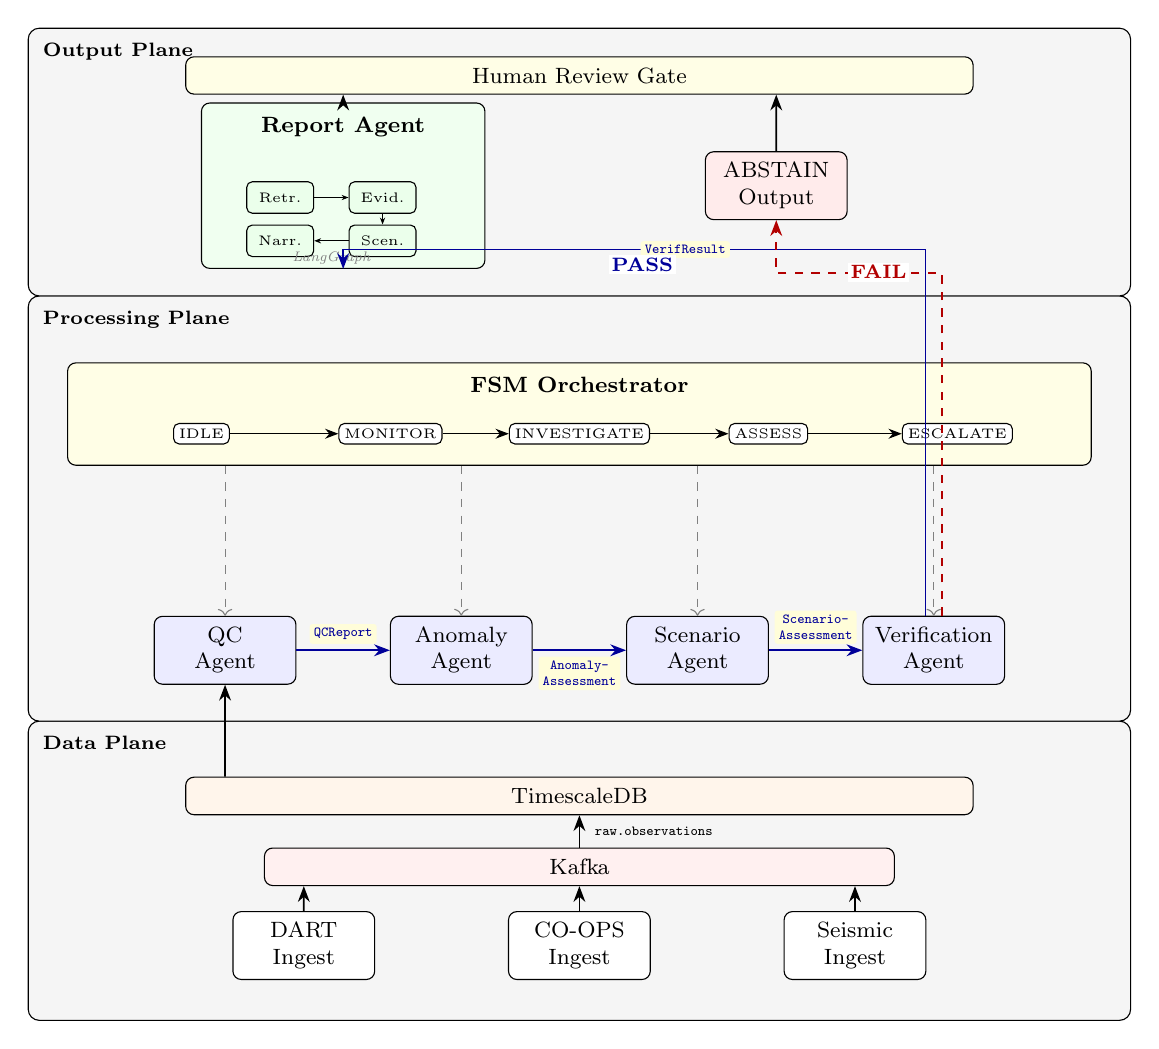
\begin{tikzpicture}[
  font=\small,
  plane/.style={draw, rounded corners=4pt, minimum width=14cm,
                fill=gray!8, inner sep=8pt},
  box/.style={draw, rounded corners=3pt, fill=white, inner sep=4pt,
              minimum width=1.8cm, align=center, font=\footnotesize},
  agent/.style={draw, rounded corners=3pt, fill=blue!8, inner sep=4pt,
                minimum width=1.8cm, align=center, font=\footnotesize},
  store/.style={draw, rounded corners=3pt, fill=orange!8, inner sep=4pt,
                minimum width=1.8cm, align=center, font=\footnotesize},
  output/.style={draw, rounded corners=3pt, fill=green!6, inner sep=4pt,
                 minimum width=1.8cm, align=center, font=\footnotesize},
  schema/.style={font=\tiny, fill=yellow!15, inner sep=1.5pt,
                 rounded corners=1pt, align=center},
  lgnode/.style={draw, rounded corners=2pt, minimum width=0.85cm,
                 minimum height=0.4cm, font=\tiny, fill=green!8,
                 align=center},
  arrow/.style={->, >=Stealth, semithick},
  seqarrow/.style={->, >=Stealth, semithick, blue!60!black},
  failarrow/.style={->, >=Stealth, semithick, red!70!black, dashed},
]

% ---- Data Plane (bottom) ----
\node[plane, minimum height=3.8cm] (data) at (0,-0.6) {};
\node[anchor=north west, font=\bfseries\scriptsize]
  at ([xshift=2pt, yshift=-2pt]data.north west) {Data Plane};

% TimescaleDB - wide persistent store at top of data plane
\node[store, minimum width=10cm] (tsdb) at (0, 0.35) {TimescaleDB};

% Kafka - event bus below TimescaleDB
\node[store, fill=red!6, minimum width=8cm] (kafka) at (0, -0.55) {Kafka};

% Ingest connectors - evenly spaced at bottom
\node[box] (dart)  at (-3.5, -1.55) {DART\\Ingest};
\node[box] (coops) at ( 0.0, -1.55) {CO-OPS\\Ingest};
\node[box] (usgs)  at ( 3.5, -1.55) {Seismic\\Ingest};

% Ingest -> Kafka (all arrows straight up)
\draw[arrow] (dart.north)  -- ([xshift=-3.5cm]kafka.south);
\draw[arrow] (coops.north) -- (kafka.south);
\draw[arrow] (usgs.north)  -- ([xshift= 3.5cm]kafka.south);

% Kafka -> TimescaleDB (vertical, with topic label)
\draw[arrow] (kafka.north) -- (tsdb.south)
  node[font=\tiny, midway, right, xshift=2pt] {\texttt{raw.observations}};

% ---- Processing Plane (middle) - agents + FSM Orchestrator ----
\node[plane, minimum height=5.4cm] (proc) at (0, 4.0) {};
\node[anchor=north west, font=\bfseries\scriptsize]
  at ([xshift=2pt, yshift=-2pt]proc.north west) {Processing Plane};

% Agents in a row - evenly spaced with room for schema labels
\node[agent] (qc)   at (-4.5, 2.2) {QC\\Agent};
\node[agent] (anom) at (-1.5, 2.2) {Anomaly\\Agent};
\node[agent] (scen) at ( 1.5, 2.2) {Scenario\\Agent};
\node[agent] (veri) at ( 4.5, 2.2) {Verification\\Agent};

% Typed handoff schema arrows between agents - alternating above/below
\draw[seqarrow] (qc.east) -- (anom.west)
  node[schema, midway, above, yshift=2pt] {\texttt{QCReport}};
\draw[seqarrow] (anom.east) -- (scen.west)
  node[schema, midway, below, yshift=-2pt] {\texttt{Anomaly-}\\\texttt{Assessment}};
\draw[seqarrow] (scen.east) -- (veri.west)
  node[schema, midway, above, yshift=2pt] {\texttt{Scenario-}\\\texttt{Assessment}};

% TimescaleDB -> QC (data flows up into processing plane)
\draw[arrow] ([xshift=-4.5cm]tsdb.north) -- (qc.south);

% FSM Orchestrator (inside Processing Plane, above agents)
\node[draw, rounded corners=3pt, fill=yellow!10, inner sep=6pt,
      minimum width=13cm, minimum height=1.3cm]
  (fsm) at (0, 5.2) {};
\node[font=\footnotesize\bfseries] at ([yshift=-8pt]fsm.north)
  {FSM Orchestrator};

% Individual state boxes inside FSM
\node[draw, rounded corners=2pt, fill=white, inner sep=2pt,
      font=\tiny] (s-idle) at (-4.8, 4.95) {IDLE};
\node[draw, rounded corners=2pt, fill=white, inner sep=2pt,
      font=\tiny] (s-mon)  at (-2.4, 4.95) {MONITOR};
\node[draw, rounded corners=2pt, fill=white, inner sep=2pt,
      font=\tiny] (s-inv)  at ( 0.0, 4.95) {INVESTIGATE};
\node[draw, rounded corners=2pt, fill=white, inner sep=2pt,
      font=\tiny] (s-ass)  at ( 2.4, 4.95) {ASSESS};
\node[draw, rounded corners=2pt, fill=white, inner sep=2pt,
      font=\tiny] (s-esc)  at ( 4.8, 4.95) {ESCALATE};
\draw[->, >=Stealth, thin] (s-idle) -- (s-mon);
\draw[->, >=Stealth, thin] (s-mon)  -- (s-inv);
\draw[->, >=Stealth, thin] (s-inv)  -- (s-ass);
\draw[->, >=Stealth, thin] (s-ass)  -- (s-esc);

% FSM -> Agents (dashed control lines to all 4 agents)
\foreach \a in {qc, anom, scen, veri} {
  \draw[gray, dashed, thin, ->] (fsm.south -| \a.north) -- (\a.north);
}

% ---- Output Plane (top) ----
\node[plane, minimum height=3.4cm] (out) at (0, 8.4) {};
\node[anchor=north west, font=\bfseries\scriptsize]
  at ([xshift=2pt, yshift=-2pt]out.north west) {Output Plane};

% Report Agent with LangGraph subgraph
\node[output, minimum width=3.6cm, minimum height=2.1cm]
  (rep) at (-3.0, 8.1) {};
\node[font=\footnotesize\bfseries, anchor=north, yshift=-2pt]
  at (rep.north) {Report Agent};
% LangGraph 4-node subgraph inside Report Agent
\node[lgnode] (lg1) at (-3.8, 7.95) {Retr.};
\node[lgnode] (lg2) at (-2.5, 7.95) {Evid.};
\node[lgnode] (lg3) at (-2.5, 7.40) {Scen.};
\node[lgnode] (lg4) at (-3.8, 7.40) {Narr.};
\node[font=\tiny\itshape, gray] at (-3.15, 7.18) {LangGraph};
\draw[-{Stealth[length=2.5pt]}, thin] (lg1) -- (lg2);
\draw[-{Stealth[length=2.5pt]}, thin] (lg2) -- (lg3);
\draw[-{Stealth[length=2.5pt]}, thin] (lg3) -- (lg4);

\node[output, fill=red!8] (abs) at ( 2.5, 8.1) {ABSTAIN\\Output};
\node[output, fill=yellow!10, minimum width=10cm] (hrg) at (0, 9.5)
  {Human Review Gate};

% Report and ABSTAIN -> HRG
\draw[arrow] (rep.north) -- ([xshift=-3.0cm]hrg.south);
\draw[arrow] (abs.north) -- ([xshift= 2.5cm]hrg.south);

% PASS/FAIL from Verification Agent to Output Plane (drawn LAST - on top)
\draw[seqarrow] ([xshift=-3pt]veri.north) -- ++(0, 4.65) -| (rep.south)
  node[schema, pos=0.25, right, xshift=2pt] {\texttt{VerifResult}};
\node[font=\scriptsize\bfseries, blue!60!black, fill=white, inner sep=1pt]
  at (0.8, 7.1) {PASS};

\draw[failarrow] ([xshift=3pt]veri.north) -- ++(0, 4.35) -| (abs.south);
\node[font=\scriptsize\bfseries, red!70!black, fill=white, inner sep=1pt]
  at (3.8, 7.0) {FAIL};

\end{tikzpicture}
\caption{System architecture and agentic pipeline. The \textbf{Data Plane}
  ingests DART, CO-OPS, and seismic observations via Kafka
  (\texttt{raw.observations} topic) into TimescaleDB (with in-memory
  fallback when the database is unavailable).
  The \textbf{Processing Plane} sequences four specialized agents (blue
  arrows) with typed Pydantic handoff schemas (yellow labels):
  QC $\to$ Anomaly Detection $\to$ Scenario Inversion $\to$ Verification.
  The \textbf{FSM Orchestrator} manages a five-state deterministic
  escalation chain (IDLE $\to$ MONITOR $\to$ INVESTIGATE $\to$ ASSESS
  $\to$ ESCALATE) and dispatches agents via control signals (gray dashed
  lines). Verification results route to either the Report Agent (PASS)
  or the fail-closed \textsc{abstain} output (FAIL, red dashed arrow).
  The Report Agent contains a four-node LangGraph subgraph
  (Retrieval $\to$ Evidence $\to$ Scenario $\to$ Narrative)
  for LLM-based advisory synthesis. In the \textbf{Output Plane}, all
  outputs pass through the mandatory Human Review Gate before
  classification as distributable; preliminary seismic-only estimates
  may be surfaced to the duty scientist sooner but remain PROVISIONAL
  and non-distributable. Any later distributable artifact must pass
  through the review-gated path (Section~\ref{sec:scenario}). The figure shows the
  target architecture; the deployed Kafka worker currently performs
  ingest, quality control, anomaly scoring, and FSM transitions, and
  fail-closes to ABSTAIN at the assessment stages.}
\label{fig:architecture}%
\label{fig:pipeline}% alias for cross-referencing both architecture and pipeline aspects
\end{figure*}

The system is organized into three planes, analogous to the
data-plane / control-plane separation in network and cloud systems
engineering (Figure~\ref{fig:architecture};
full UML diagrams in Appendix~\ref{sec:appendix-uml}).
The agentic pipeline sequences four processing agents under
deterministic FSM control, with typed Pydantic schemas enforcing
inter-agent handoff contracts; a fifth agent (Report) is triggered
by verification routing (Figure~\ref{fig:pipeline}).

\paragraph{Data Plane.}
Three ingest connectors poll external NOAA and USGS endpoints at
configurable poll cycles (DART: 60\,s standard / 15\,s event mode;
CO-OPS: 30\,s; USGS seismic: 15\,s);
the full DART and CO-OPS station network is shown in
Appendix~\ref{sec:appendix-coops}. Note that standard-mode DART
Bottom Pressure Recorder (BPR) data arrives in 6-hour batches of 24~observations at 15\,min
intervals; the 60\,s poll cycle detects mode transitions promptly. Each connector canonicalizes
records into validated Pydantic schemas, computes a SHA-256 payload
hash, appends to an in-memory buffer, and (when a database is configured)
persists the raw observation to TimescaleDB; records that fail schema
validation are quarantined. The payload hash is carried in the
\texttt{InputRef} field of handoff schemas where populated; end-to-end
provenance propagation from raw ingest to the escalation packet is not yet
complete.

\paragraph{Processing Plane.}
The deterministic FSM orchestrator advances through five states
(IDLE, MONITOR, INVESTIGATE, ASSESS, ESCALATE) based on anomaly scores
and seismic event parameters (Section~\ref{sec:fsm}). Four specialized
agents (QC, Anomaly, Scenario, Verification) execute sequentially.
Each agent exposes a single typed entrypoint, returns a Pydantic
schema, and cannot modify agent state outside its schema output. Agent
permissions are specified by a machine-readable YAML policy. The policy
is a declarative contract evaluated on demand through a queryable
internal endpoint; nothing in the pipeline execution path consults it,
and it is not wired as an enforcing interceptor
(Section~\ref{sec:safety}).

\paragraph{Output Plane.}
The Report Agent generates structured probabilistic assessments in three
tiers. The ABSTAIN output node produces an explicit abstention document
when verification fails. All verified outputs (reports and abstentions alike)
are presented at the Human Review Gate, which is the precondition for
any future classification as
\texttt{APPROVED\_INTERNAL}; preliminary seismic-only estimates
may be surfaced to the duty scientist sooner, but remain
\texttt{PROVISIONAL} and non-distributable. Any later distributable
artifact must pass through the review-gated path
(Section~\ref{sec:scenario}).

\paragraph{Cross-cutting concerns.}
An OpenTelemetry~\citep{opentelemetry2024} span wraps each pipeline
run in the API and the deployed worker, exported to Jaeger when an OTLP
endpoint is configured; finer-grained per-agent spans are future work. The observability stack (Prometheus, Grafana,
Jaeger) is deployed; a Prometheus \texttt{/metrics} endpoint reports
the current FSM state plus domain counters (ingest outcomes, anomaly
scores, FSM transitions, abstains, verification outcomes, guardrail
scans) and a per-station scoring-latency histogram, with broader
end-to-end latency histograms left to future work. Every significant
system event is appended to an append-only audit log, held in memory
and persisted to TimescaleDB when a database is configured
(Section~\ref{sec:audit}).

\paragraph{Deployment.}
The system runs as a Docker Compose stack: TimescaleDB (PostgreSQL 16 +
TimescaleDB 2.17), Apache Kafka (KRaft single-broker), Prometheus,
Grafana, Jaeger, a core FastAPI server, three ingest workers, a
pipeline worker, and a Mission Control React dashboard with a FastAPI
backend-for-frontend. The API surface is secured by API key
authentication.

\paragraph{Mission Control dashboard.}
A browser-based dashboard (Figure~\ref{fig:dashboard-layout},
Appendix~\ref{sec:appendix-dashboard}) provides real-time situational
awareness via a WebSocket connection streaming FSM state, anomaly
scores, and audit entries.  The interface is organized into a
three-column grid: FSM state visualization with transition history, a
Pacific Ocean map with station markers and epicenter annotation (an
anomaly score time-series with threshold annotations ($T_1$, $T_2$,
$T_3$) is embedded along the map's lower edge), a Human Review Gate
for APPROVE/REJECT/DEFER decisions, a component registry, an active
event panel, and an append-only audit log.  Dashboard displays are read-only; the sole write path is the
Human Review Gate, which issues decisions through a separate
service-authenticated REST endpoint. Reviewer identity on that
endpoint is caller-asserted and is recorded as such
(\texttt{CALLER\_ASSERTED}) in the tamper-evident decision record;
per-reviewer authentication is future work.

\paragraph{Envisioned near-real-time operational flow.}
The following describes the design-target operational mode, which
has been validated only on archived data (Section~\ref{sec:evaluation});
the deployed worker already runs ingest, QC, anomaly scoring, and FSM
transitions on live streams, while full live assessment operation
(Scenario, Verification, Report) remains future work.
In the target operational mode, the seismic connector detects a
qualifying earthquake within 15\,s of USGS publication. The FSM
transitions to MONITOR. The DART connector polls standard-mode feeds
at 60\,s and, once a station is observed in event mode, polls that
station at 15\,s for low-latency follow-up. DART event packets may
include an initial 15\,s burst followed by sustained 1-minute averages;
each new observation flows through QC and anomaly scoring within a single
poll cycle (design target: under one second for QC and ensemble
scoring). When anomaly thresholds are crossed, scenario inversion
is triggered asynchronously; the NNLS solve plus 500-iteration
bootstrap targets completion within three minutes
(Section~\ref{sec:discussion}).
The retrospective evaluation in Section~\ref{sec:evaluation}
validates the signal-processing pipeline on archived DART data.

% ============================================================
%  4. Methods
% ============================================================

\section{Methods}
\label{sec:methods}

\subsection{Data Ingestion and Quality Control}
\label{sec:qc}

The QC Agent applies five QARTOD-aligned checks to every incoming
observation as it enters the detection pipeline. The resulting flags
annotate the record for the audit trail and operator review; they do
not filter observations out of anomaly scoring, because a genuine
tsunami signal trips several of these checks:

\begin{description}[leftmargin=1.5em]
  \item[Timing check.] Verifies that the observation timestamp
    advances by the expected interval (15\,min for standard-mode DART,
    60\,s for CO-OPS one-minute product). Gaps exceeding $2\times$ the
    expected interval cause the record to be flagged.

  \item[Gross range check.] Rejects values outside configured QC
    bounds.  For CO-OPS, water levels outside $\pm3$\,m from the STND
    datum are flagged, with a $1.5\times$ SUSPECT range.  For DART,
    gross range applies to detided residuals ($\pm0.5$\,m); raw
    water-column heights bypass this check pending the detiding
    pipeline.  The ingest layer applies a \texttt{math.isfinite()}
    guard that rejects NaN and Inf values; NDBC 9999.000\,m
    missing-data sentinels are filtered at parse time
    (see Section~\ref{sec:eval-detiding}).

  \item[Spike check.] Flags observations whose absolute deviation
    from the previous value exceeds a fixed threshold (0.1\,m for
    DART, 0.3\,m for CO-OPS), with a $2\times$ SUSPECT range.  This
    is a simplified 2-point test; the full QARTOD 3-point median test
    is deferred to a future calibration milestone.

  \item[Rate-of-change check.] Rejects records for which
    $|\Delta h / \Delta t|$ exceeds a configurable maximum rate
    (0.001\,m\,s$^{-1}$ for DART, 0.005\,m\,s$^{-1}$ for CO-OPS).
    The QARTOD standard uses rolling standard-deviation-based
    thresholds; fixed thresholds are an interim simplification pending
    calibration with operational data.

  \item[Flat-line check.] Flags stations whose total value variation
    (max $-$ min) within a rolling 1-hour window falls below a minimum
    threshold (0.0001\,m for DART, 0.001\,m for CO-OPS), indicating
    sensor lock or transmission failure.  Returns SUSPECT only; a FAIL
    tier is deferred to future calibration.
\end{description}

A \textbf{station confidence score} $c \in [0,1]$ is computed per
observation as $c = 1 - (0.3\, n_{\text{suspect}} + 1.0\, n_{\text{fail}})
/ n_{\text{tests}}$, where $n_{\text{tests}}$ counts only evaluated
checks (excluding \texttt{NOT\_APPLICABLE}, \texttt{NOT\_EVALUATED},
and \texttt{MISSING}).
Records with $c < 0.5$ are marked \texttt{record\_usable: false}.
The flag is advisory: anomaly scoring deliberately consumes all records
regardless, because a genuine tsunami signal trips the same spike and
rate-of-change checks. The deployed worker summarizes each batch's QC
into the audit trail (record and usable counts, minimum confidence, and
the number of records whose checks produced no definitive result).

\subsection{Anomaly Detection}
\label{sec:anomaly}

The Anomaly Agent produces an ensemble score $s \in [0,1]$ from
three core components and one optional ML component.

\paragraph{Pre-processing.}
Raw water-level observations $\eta(t)$ are first detided by fitting
a harmonic model over a 30-day rolling window:
\begin{equation}
  \hat{\eta}_T(t) = \bar{\eta} + \sum_{k=1}^{8}
    A_k \cos\!\bigl(\omega_k t + \phi_k\bigr),
  \label{eq:tidal}
\end{equation}
where the eight constituents are M2, S2, N2, K1, O1, P1, K2, Q1,
fit by iteratively reweighted least squares (IRLS) with Cauchy
weights following~\citet{codiga2011unified}, building on the classical
harmonic framework of~\citet{pawlowicz2002classical}.
We choose harmonic analysis over the cubic-polynomial extrapolation
used by NOAA's operational Tsunami Detection Algorithm~\citep{mofjeld1997tsunami}
because harmonic decomposition yields physically interpretable
constituent amplitudes (M2, S2, etc.) that enable quantitative
validation of detiding quality (Section~\ref{sec:eval-detiding}).
This approach corresponds to Method~1 in the five-method comparison
of~\citet{percival2015detiding}, who found that RMSE varies over two
orders of magnitude among detiding methods; the Mofjeld polynomial
requires only 3~hours of prior data but trades waveform
characterization accuracy for speed.
The Mofjeld polynomial remains operational in NOAA's
Tsunami Detection Algorithm~\citep{mofjeld1997tsunami} due
to its minimal data requirements;
we accept the 30-day calibration constraint in exchange for
physically interpretable constituent amplitudes.
The fit window spans 30 days of pre-event standard-mode data,
which cleanly resolves the six dominant constituents per the
Rayleigh criterion; the closely spaced P1--K1 and K2--S2 pairs require
${\sim}183$~days but have small deep-ocean amplitudes.
The detided residual $r(t) = \eta(t) - \hat{\eta}_T(t)$ is then
bandpass-filtered with a causal 4th-order Butterworth filter
(forward-only IIR, initialized with steady-state conditions;
passband $0.000139$--$0.00333$\,Hz, corresponding to 5--120\,min periods)
to isolate the tsunami frequency band.  The causal (forward-only)
implementation ensures that the filtered value at time $t$ depends
only on observations at or before $t$, as required for real-time
processing where future data is unavailable.

\paragraph{Residual post-processing.}
The evaluation figures (Section~\ref{sec:eval-tohoku} and Appendix~\ref{sec:appendix-case-studies})
display detided residuals produced by the offline extraction pipeline
summarized in Algorithm~\ref{alg:residual}.  This pipeline applies
despike filtering, tidal removal via IRLS, pre-event linear detrend, an
optional rolling-median baseline correction (window size depends on
epicentral distance and event), and Hampel spike cleaning.

\begin{algorithm}[t]
\caption{Detided Residual Extraction}
\label{alg:residual}
\begin{algorithmic}[1]
\REQUIRE Raw height record $\eta(t)$, calibration window $\eta_\text{cal}$
\ENSURE Detided residual $r(t)$, bandpass-filtered signal $r_\text{bp}(t)$
\STATE \COMMENT{\textit{Stage 1: Clean calibration data}}
\STATE $\eta'_\text{cal} \leftarrow \text{Hampel}(\eta_\text{cal},\;
  h_w{=}3,\; 3\sigma_\text{MAD})$
  \COMMENT{spike removal}
\STATE Detect gaps where $\Delta t > 6 \times \text{median}(\Delta t)$;
  correct level shifts across gaps
\STATE Remove linear drift from $\eta'_\text{cal}$ via $\text{polyfit}(\deg{=}1)$
\STATE \COMMENT{\textit{Stage 2: Fit tidal harmonics}}
\STATE $\hat{\eta}_T(t) \leftarrow \text{IRLS-fit}(\eta'_\text{cal})$
  \COMMENT{8 constituents, Cauchy weights}
\STATE \COMMENT{\textit{Stage 3: Detide event data}}
\STATE $r(t) \leftarrow \eta(t) - \hat{\eta}_T(t)$
  \COMMENT{broadband residual}
\STATE $r_\text{bp}(t) \leftarrow \text{Butterworth}(r,\; 5\text{--}120\;\text{min},\;
  \text{4th order, causal})$
\RETURN $r(t),\; r_\text{bp}(t)$
\end{algorithmic}
\end{algorithm}

\paragraph{Component 1: Threshold score $s_\text{thr}$.}
The filtered peak amplitude $A_\text{max}$ is compared with a
station-specific threshold $\theta$:
\begin{equation}
  s_\text{thr} = \min\!\Bigl(1,\;
    \max\!\bigl(0,\; A_\text{max}/\theta - 1\bigr)\Bigr).
\end{equation}
The score is zero when $A_\text{max} \leq \theta$ and ramps linearly
to~1 at $A_\text{max} = 2\theta$. Sub-threshold amplitudes contribute
nothing to the ensemble, preventing false inflation from background
noise. In quiet periods (no M$\geq$6.5 event within 90\,min),
$\theta$ is inflated by 30\% to reduce the false-alarm rate.

\paragraph{Component 2: Wavelet score $s_\text{wav}$.}
A Daubechies-4 (db4) discrete wavelet transform~\citep{daubechies1992ten}
decomposes the bandpass-filtered detided residual into subbands. Coefficients at scales corresponding
to the 5--120\,min tsunami band are squared and summed to form a
tsunami-band energy $E_\text{tsun}$. The score is:
\begin{equation}
  s_\text{wav} = \max\!\left(0,\;
    1 - \frac{E_\text{base}}{E_\text{tsun}}\right),
\end{equation}
where $E_\text{base}$ is the wavelet energy in the same subband computed from
a pre-calibrated non-event baseline. Decomposition depth is adjusted
for the sampling interval (level~6 for 60-second data, level~8 for
15-second data), and only detail levels overlapping the 5--120-minute
band contribute to $E_\text{tsun}$.
The score is zero when
$E_\text{tsun} \leq E_\text{base}$ and approaches~1 as the tsunami-band
energy dominates.

\paragraph{Component 3: BOCPD score $s_\text{bcp}$.}
We apply the BOCPD algorithm~\citep{adams2007bayesian} to the
broadband detided residual.
The algorithm maintains a run-length distribution using a
Normal-Gamma conjugate prior and constant hazard function
($\lambda = 1/300$, corresponding to an expected run length of
300~samples).
The physical rationale is that tsunami onset manifests as a
distributional shift in the broadband residual before the full
narrowband oscillatory waveform develops within the 5--120\,min
passband.  Under constant hazard, the marginal posterior $P(r_t{=}0
\mid x_{1:t})$ is dominated by the prior hazard rate and provides
little discrimination between changepoint and steady-state
observations; we therefore use \emph{predictive surprise} (the
negative log-evidence $-\log P(x_t \mid x_{1:t-1})$) as the
detection signal, which spikes when an observation is inconsistent
with the model learned from recent data.  The robust baseline
(median and MAD) is computed from surprise values preceding the peak,
preventing post-changepoint inflation of the scale estimate.
To prevent false positive scores on stationary data, the expected maximum
z-score for $n$ i.i.d.\ Gaussian samples,
$\sqrt{2\ln n}\,/\,0.6745$ (in MAD units), is subtracted; only the
excess $z_\text{excess}$ is scored via a saturating function
$s_\text{bcp} = z_\text{excess}\,/\,(z_\text{excess} + 5)$,
yielding $s_\text{bcp} \in [0,1]$.  This is particularly valuable for DART
standard-mode data (15\,min sampling), where Nyquist constraints
render the bandpass filter ineffective.
The constant-hazard BOCPD model assumes observations within each
run-length segment are i.i.d.\ Gaussian.  Detided ocean residuals
exhibit autocorrelation (imperfect tidal removal, ocean dynamics),
violating this assumption and potentially inflating surprise scores.
The hazard rate $\lambda = 1/300$ was chosen empirically; smaller
values delay detection and larger values increase false alarms.
The run-length distribution is truncated at 600 samples for
computational efficiency, introducing approximation error for very
long stationary segments.

\paragraph{Component 4: Spatial coherence score $s_\text{coh}$.}
For each pair of stations $(i, j)$, the expected inter-station
travel time is estimated as $\tau_{ij} = d_{ij} / c_\text{sw}$,
where $d_{ij}$ is the great-circle distance and $c_\text{sw} \approx
198$\,m\,s$^{-1}$ is the long-wave (shallow-water) phase speed
for a mean ocean depth of ${\sim}4$\,km. A
station $j$ is counted as \emph{confirming} if its anomaly onset
falls within $\pm 20\%$ of $\tau_{ij}$ relative to station $i$.
The score is $s_\text{coh} = \min(1,\; n_\text{confirm} / n_\text{min})$,
where $n_\text{min} = 2$ is the minimum confirming-station threshold.
Using $\tau_{ij} = d_{ij}/c_\text{sw}$ assumes the source lies on the
extension of the station baseline: by the triangle inequality it is
the largest delay a common source can produce, and for a source
offset in azimuth the true delay is smaller.  The check is therefore
sufficient but not necessary, and coherent arrivals at pairs well off
the source axis will not confirm.  This affects no reported number,
since $s_\text{coh}$ enters only the Isolation Forest feature vector
and that model is never loaded.

\paragraph{Ensemble fusion.}
The ensemble uses three core components plus one optional ML
component. The spatial coherence score $s_\text{coh}$ is not
weighted directly in the sum; it serves as an input feature to the
Isolation Forest (alongside short-period energy and rate-of-change
features), which produces the ML anomaly score $s_\text{ml}$.
When the Isolation Forest model is available:
\begin{equation}
  s = \alpha_1\, s_\text{thr}
    + \alpha_2\, \max(s_\text{wav},\, s_\text{bcp})
    + \alpha_3\, s_\text{ml},
  \label{eq:ensemble}
\end{equation}
with $(\alpha_1, \alpha_2, \alpha_3) = (0.50, 0.35, 0.15)$.
When the ML component is unavailable (the default configuration),
the ensemble reduces to:
\begin{equation}
  s = \alpha_1'\, s_\text{thr}
    + \alpha_2'\, \max(s_\text{wav},\, s_\text{bcp}),
  \label{eq:ensemble_noml}
\end{equation}
with $(\alpha_1', \alpha_2') = (0.588, 0.412)$, obtained by
renormalizing $(\alpha_1, \alpha_2)$ over the two remaining
components.
Algorithm~\ref{alg:scoring} summarizes the per-window scoring procedure.

\begin{algorithm}[t]
\caption{Ensemble Anomaly Scoring (per sliding window)}
\label{alg:scoring}
\begin{algorithmic}[1]
\REQUIRE Bandpass-filtered signal $r_\text{bp}(t)$, broadband residual $r(t)$,
  station threshold $\theta$, baseline wavelet energy $E_\text{base}$,
  BOCPD hazard $\lambda$
\ENSURE Ensemble score $s \in [0,1]$
\STATE $A_\text{max} \leftarrow \max|r_\text{bp}|$
\STATE $s_\text{thr} \leftarrow \min(1,\;\max(0,\; A_\text{max}/\theta - 1))$
  \COMMENT{threshold on filtered signal}
\STATE $E_\text{tsun} \leftarrow \text{DWT tsunami-band energy}(r_\text{bp})$
\STATE $s_\text{wav} \leftarrow \max(0,\; 1 - E_\text{base}/E_\text{tsun})$
  \COMMENT{wavelet on filtered signal}
\STATE $s_\text{bcp} \leftarrow \text{BOCPD surprise}(r,\; \lambda{=}1/300)$
  \COMMENT{changepoint on broadband residual}
\STATE $s \leftarrow 0.588\, s_\text{thr} + 0.412\, \max(s_\text{wav},\, s_\text{bcp})$
  \COMMENT{Eq.~\ref{eq:ensemble_noml}}
\RETURN $s$
\end{algorithmic}
\end{algorithm}

\paragraph{Rayleigh wave false-trigger detection.}
DART Bottom Pressure Recorders enter event mode when pressure
deviation exceeds approximately 30\,mm from the predicted
value~\citep{bernard2011history}.
After a large earthquake, seismic Rayleigh surface waves can cause
transient seafloor pressure perturbations exceeding this threshold,
producing a false event-mode trigger.  The detection algorithm's own
documentation anticipates this, noting that a DART gauge would be set
into rapid reporting mode by the first group of Rayleigh
waves~\citep{mofjeld1997tsunami}. This is an amplitude/timing
mechanism, not spectral: Rayleigh waves from typical crustal earthquakes
have dominant periods of 10--50\,s~\citep{lay1995modern}; for great
earthquakes ($M_w > 8.5$), significant energy extends to 100--300\,s,
overlapping the lower edge of the 5--120\,min tsunami passband
(see the far-field seismic contamination in
Section~\ref{sec:eval-tohoku}).
Detection therefore relies on timing correlation with the
earthquake epicenter rather than spectral separation. The expected Rayleigh arrival time is
$t_R = d / v_R$ where $d$ is the haversine distance and
$v_R \approx 3.6$\,km/s is the oceanic Rayleigh wave group
velocity at ${\sim}20$\,s dominant period~\citep{lay1995modern}.
\citet{kubota2020ultrabroadband} provide detailed analysis of Rayleigh
wave pressure signals in ocean-bottom records, confirming the velocity
range used here. A spike is flagged as suspect if
$|t_\text{actual} - t_R| / t_R \leq 0.20$ and $d \leq 3{,}000$\,km
(an engineering threshold: beyond this distance, Rayleigh wave
amplitude attenuates below the DART 30\,mm event-mode trigger for
all but the very largest earthquakes).
This check always produces CONCERN, never FAIL: timing correlation
is not proof of false trigger, as real tsunamis also follow large
earthquakes.

\subsection{Orchestration: Deterministic FSM}
\label{sec:fsm}

The FSM advances through five states according to the scheme in
Figure~\ref{fig:fsm}. A seismic event with $M \geq M_\text{min}$
(default 6.0) whose region lies in a tsunamigenic zone triggers the
transition IDLE $\to$ MONITOR; an event outside those zones does not
leave IDLE regardless of magnitude. All
subsequent transitions are driven by the ensemble anomaly score $s$
relative to three configurable thresholds: $T_1 = 0.35$,
$T_2 = 0.60$, $T_3 = 0.85$ (Table~\ref{tab:fsm}).
These thresholds are design constants chosen to provide
progressive escalation with meaningful separation between stages;
$T_3$ is intentionally high to reduce false escalation (see
Limitation~6 in Section~\ref{sec:discussion} for calibration status).

\begin{table}[t]
\centering
\caption{FSM state transitions. De-escalation (downward) occurs when
  the score drops below the corresponding lower threshold.}
\label{tab:fsm}
\begin{tabular}{llll}
\toprule
From & To & Trigger & De-escalation \\
\midrule
IDLE        & MONITOR     & Seismic $M \geq M_\text{min}$ in a tsunamigenic zone & N/A \\
MONITOR     & IDLE        & Timeout (12\,h) AND $s < T_1$ & --- \\
MONITOR     & ESCALATE    & Seismic-only$^\ddagger$        & --- \\
MONITOR     & INVESTIGATE & $s \geq T_1 = 0.35$ OR override$^*$ & $s < T_1$ $\to$ MONITOR \\
INVESTIGATE & ASSESS      & $s \geq T_2 = 0.60$           & $s < T_1$ $\to$ MONITOR$^*$ \\
ASSESS      & ESCALATE    & $s \geq T_3 = 0.85$           & $s < T_2$ $\to$ INVESTIGATE \\
ASSESS      & ESCALATE    & Seismic override$^\dagger$    & --- \\
ESCALATE    & IDLE        & Explicit event resolution$^\S$ & --- \\
\bottomrule
\end{tabular}
\end{table}
{\footnotesize $\dagger$ Seismic override: $M \geq 7.5$ AND DART stations
reporting event-mode transmissions.\\
$\ddagger$ Seismic-only escalation: $M \geq 7.5$ AND depth $< 100$\,km;
fires as a chained IDLE$\to$MONITOR$\to$ESCALATE transition,
not from a standing MONITOR state.
No DART data required (per PTWC/JMA operational criteria).\\
$*$ The seismic override condition ($M \geq 7.5$ with DART event-mode
activation) prevents a sub-$T_1$ ensemble score from holding the FSM
back: from MONITOR it advances to INVESTIGATE, and de-escalation from
INVESTIGATE is suppressed (the FSM advances to ASSESS instead), so a
low interim ensemble score cannot hold down or de-escalate an event
with a large earthquake and active event-mode DART reporting.\\
$\S$ Explicit event resolution is implemented as
\texttt{resolve\_event()}. No current API route invokes it, and the
caller-asserted review decisions (APPROVE, REJECT, DEFER) are all
recorded without changing FSM state.\\
See Appendix~\ref{sec:appendix-fsm} for the complete transition rule
specification.}

\begin{figure}[t]
\centering
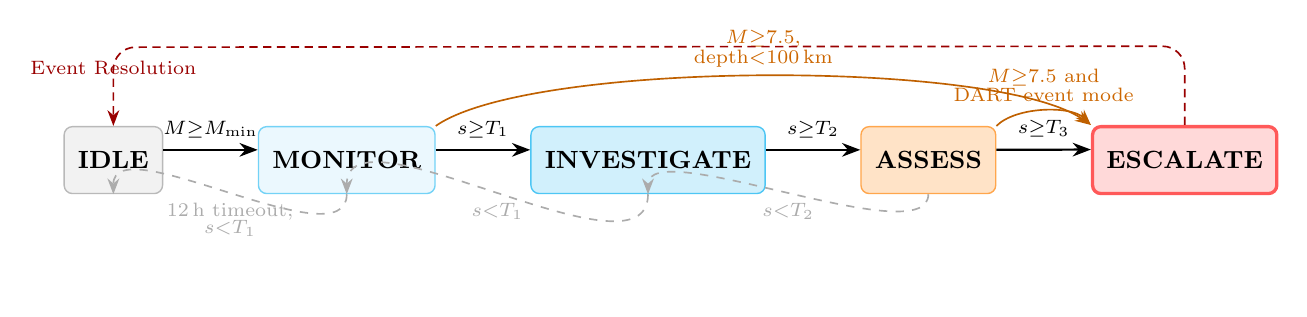
\begin{tikzpicture}[
  font=\small,
  % ---- State node styles (severity-coded rounded rectangles) ----
  base/.style={draw, rectangle, rounded corners=3pt,
    minimum height=0.85cm, align=center, inner sep=5pt,
    text depth=0pt, line width=0.5pt},
  Sidle/.style={base, fill=gray!10,   draw=gray!55},
  Smon/.style ={base, fill=cyan!8,    draw=cyan!55},
  Sinv/.style ={base, fill=cyan!18,   draw=cyan!70},
  Sass/.style ={base, fill=orange!22, draw=orange!70},
  Sesc/.style ={base, fill=red!15,    draw=red!65, line width=1.2pt},
  % ---- Arrow styles ----
  fwd/.style ={->, >=Stealth, thick},
  bwd/.style ={->, >=Stealth, semithick, dashed, gray!65},
  hres/.style={->, >=Stealth, semithick, densely dashed, red!60!black},
  seis/.style={->, >=Stealth, semithick, orange!75!black},
  lbl/.style ={font=\scriptsize, inner sep=1pt},
]
% ---- States (1.2 cm gaps give forward-arrow labels room to breathe) ----
\node[Sidle] (idle)                      {\textbf{IDLE}};
\node[Smon]  (mon) [right=1.2cm of idle] {\textbf{MONITOR}};
\node[Sinv]  (inv) [right=1.2cm of mon]  {\textbf{INVESTIGATE}};
\node[Sass]  (ass) [right=1.2cm of inv]  {\textbf{ASSESS}};
\node[Sesc]  (esc) [right=1.2cm of ass]  {\textbf{ESCALATE}};

% ---- Escalation transitions ----
%  Connect at 35% down from node top (draw.io exitY/entryY=0.35), keeping
%  them visually above center and well clear of the de-escalation arrows below.
\draw[fwd]
  ($(idle.north east)!0.35!(idle.south east)$) --
  node[lbl, midway, above=3pt]{$M{\geq}M_\text{min}$}
  ($(mon.north west)!0.35!(mon.south west)$);
\draw[fwd]
  ($(mon.north east)!0.35!(mon.south east)$) --
  node[lbl, midway, above=3pt]{$s{\geq}T_1$}
  ($(inv.north west)!0.35!(inv.south west)$);
\draw[fwd]
  ($(inv.north east)!0.35!(inv.south east)$) --
  node[lbl, midway, above=3pt]{$s{\geq}T_2$}
  ($(ass.north west)!0.35!(ass.south west)$);
\draw[fwd]
  ($(ass.north east)!0.35!(ass.south east)$) --
  node[lbl, midway, above=3pt]{$s{\geq}T_3$}
  ($(esc.north west)!0.35!(esc.south west)$);

% ---- Seismic override: ASSESS -> ESCALATE ----
%  Shallow arc via corner anchors (draw.io: single waypoint ~30 px above nodes).
\draw[seis] (ass.north east) to[out=45, in=135, looseness=0.75]
  node[lbl, above=2pt, align=center, text=orange!80!black]
    {$M{\geq}7.5$ and\\[-1pt]DART event mode} (esc.north west);

% ---- Seismic-only escalation: MONITOR -> ESCALATE ----
\draw[seis] (mon.north east) to[out=35, in=145, looseness=0.45]
  node[lbl, above=2pt, align=center, text=orange!80!black]
    {$M{\geq}7.5$,\\[-1pt]depth${<}100$\,km} (esc.north west);

% ---- De-escalation transitions (below node row) ----
%  Smooth U-arcs (out=270, in=90) staggered by looseness so each arc has
%  a distinct depth; label at midway sits at the arc bottom.
\draw[bwd] (ass.south) to[out=270, in=90, looseness=0.55]
  node[lbl, midway, below=2pt]{$s{<}T_2$} (inv.south);
\draw[bwd] (inv.south) to[out=270, in=90, looseness=0.80]
  node[lbl, midway, below=2pt]{$s{<}T_1$} (mon.south);
\draw[bwd] (mon.south) to[out=270, in=90, looseness=0.75]
  node[lbl, midway, below=2pt, align=center]{12\,h timeout,\\[-2pt]$s{<}T_1$}
  (idle.south);

% ---- Human resolution: ESCALATE -> IDLE ----
%  Trapezoidal arch matching draw.io waypoints (680,160)->(560,140)->(240,140)->(120,160):
%  rises steeply from ESCALATE, runs flat well above all nodes, descends to IDLE.
\draw[hres, rounded corners=8pt]
  (esc.north) -- ++(0, 1.0cm)
  -- ($(idle.north)+(0, 1.0cm)$) -- (idle.north)
  node[lbl, pos=0.5, above=3pt, text=red!60!black]{Event Resolution};
\end{tikzpicture}
\caption{\textbf{FSM state diagram.}
  Solid black arrows: escalation driven by seismic magnitude~$M$ or
  ensemble anomaly score~$s$.
  Dashed gray arrows: de-escalation when the score drops below the
  corresponding lower threshold ($T_1$ or $T_2$); \textsc{monitor}
  also returns to \textsc{idle} after a 12\,h timeout if $s < T_1$.
  Orange arcs: seismic-only escalation ($M \geq 7.5$, depth $< 100$\,km)
  bypasses \textsc{investigate}/\textsc{assess} entirely;
  seismic override ($M \geq 7.5$ and DART event mode)
  bypasses $T_3$ from \textsc{assess} (the same override also advances
  \textsc{monitor} and \textsc{investigate} one state per evaluation;
  arcs omitted for clarity).
  Red dashed arc: explicit event resolution, the only exit from
  \textsc{escalate}. No API route invokes it today.
  Thresholds: $T_1{=}0.35$, $T_2{=}0.60$, $T_3{=}0.85$.}
\label{fig:fsm}
\end{figure}

Each transition is recorded as an append-only \texttt{TransitionRecord}
containing the transition ID, UTC timestamp, event ID, pipeline trace
ID, from/to states, trigger reason, anomaly score, seismic magnitude,
and the threshold configuration in effect at the time of the
transition. The FSM is not thread-safe internally; the FastAPI
application serializes all FSM access via a single lock.
Algorithm~\ref{alg:fsm} formalizes the transition logic.

\begin{algorithm}[t]
\caption{FSM State Transition}
\label{alg:fsm}
\begin{algorithmic}[1]
\REQUIRE Current state $q$, ensemble score $s$, seismic event $e$
  (magnitude $M$, depth $d$, DART event-mode flag), elapsed time $\Delta t$
\ENSURE Next state $q'$
\IF{$q = \textsc{idle}$ \AND $e$ with $M \geq M_\text{min}$ \AND region $\in$ tsunamigenic zones}
  \STATE $q' \leftarrow \textsc{monitor}$ \COMMENT{seismic trigger}
  \IF{$M \geq 7.5$ \AND $d < 100$\,km}
    \STATE $q' \leftarrow \textsc{escalate}$ \COMMENT{seismic-only chain}
  \ENDIF
  \RETURN $q'$
\ELSIF{$q = \textsc{monitor}$}
  \IF{$s \geq T_1$} \RETURN \textsc{investigate}
  \ELSIF{$M \geq 7.5$ \AND event-mode}
    \RETURN \textsc{investigate} \COMMENT{seismic override prevents holding}
  \ELSIF{$\Delta t > 12$\,h \AND $s < T_1$} \RETURN \textsc{idle}
  \ENDIF
\ELSIF{$q = \textsc{investigate}$}
  \IF{$s \geq T_2$} \RETURN \textsc{assess}
  \ELSIF{$M \geq 7.5$ \AND event-mode}
    \RETURN \textsc{assess} \COMMENT{seismic override prevents holding or de-escalation}
  \ELSIF{$s < T_1$} \RETURN \textsc{monitor}
  \ENDIF
\ELSIF{$q = \textsc{assess}$}
  \IF{$s \geq T_3$ \OR ($M \geq 7.5$ \AND event-mode)}
    \RETURN \textsc{escalate}
  \ELSIF{$s < T_2$} \RETURN \textsc{investigate}
  \ENDIF
\ELSIF{$q = \textsc{escalate}$}
  \IF{explicit event resolution} \RETURN \textsc{idle}
  \ENDIF
\ENDIF
\RETURN $q$ \COMMENT{no transition}
\end{algorithmic}
\end{algorithm}

\subsection{Scenario Inversion}
\label{sec:scenario}

When the FSM reaches ASSESS or ESCALATE, the Scenario Agent performs
NNLS inversion~\citep{lawson1974solving, percival2011extraction} against
a unit-source database following the SIFT
methodology~\citep{gica2008development}.  The unit-source database is a
declared interface, and the implementation shipped with the release
holds caller-supplied synthetic waveforms for development and testing
rather than physics-based propagation solutions.  Operational use
requires a real propagation database such as the NOAA NCTR Forecast
Propagation Database.  No amplitude reported in this paper comes from
the inversion; see Limitations.

\paragraph{Inversion.}
Let $\mathbf{d} \in \mathbb{R}^N$ be the stacked observation vector
(water-level anomalies at $S$ stations, each sampled at $T$ time points,
so $N = S \times T$) and $\mathbf{H} \in \mathbb{R}^{N \times K}$ the
Green's function matrix whose $k$-th column is the predicted observation
vector for unit-source scenario $k$.
The inversion solves:
\begin{equation}
  \hat{\mathbf{m}} = \underset{\mathbf{m} \geq \mathbf{0}}
    {\arg\min}\;\|\mathbf{H}\mathbf{m} - \mathbf{d}\|_2^2,
  \label{eq:nnls}
\end{equation}
using the active-set algorithm of~\citet{lawson1974solving} as
implemented in \texttt{scipy.optimize.nnls}. The non-negativity
constraint is physically motivated: each weight scales a
pre-computed unit-source response that embeds the fault geometry,
so negative weights would imply unphysical reversal of slip sense.

\paragraph{Uncertainty quantification.}
Uncertainty in $\hat{\mathbf{m}}$ is quantified via $B=500$ bootstrap
iterations using station resampling: at each iteration, $S$ stations are
drawn with replacement from the original $S$, the corresponding row-blocks
of $\mathbf{H}$ and $\mathbf{d}$ are reassembled, and NNLS is re-solved.
The resulting ensemble $\{\hat{\mathbf{m}}^{(b)}\}_{b=1}^B$
yields P10/P50/P90 coastal amplitude envelopes for each scenario.

\paragraph{Constraint stages.}
The inversion operates in three constraint stages:
\texttt{SEISMIC\_ONLY} (magnitude scaling, no DART data),
\texttt{DART\_CONSTRAINED} (initial DART waveform onset), and
\texttt{MULTI\_STATION} (multiple DART stations providing tighter
constraints). The active stage is recorded in the
\texttt{ScenarioAssessment} schema and propagated to the final report.

\paragraph{Seismic-only estimate.}
When the FSM enters MONITOR and no DART data are yet available, a
lightweight seismic-only estimate is produced using magnitude scaling
alone.  Surface rupture length follows the all-fault-type regression
of~\citet{wells1994new} (calibrated for crustal earthquakes up to
$M_w {\sim}8$; extrapolation to giant
subduction megathrust earthquakes requires caution; for example,
the regression predicts $L \approx 1{,}150$\,km for $M_w$\,9.1,
whereas the 2011 T\={o}hoku rupture was ${\sim}450$\,km);
slip is derived from an approximate power-law parameterization
that requires regional calibration before operational use.
This output carries a mandatory label: \emph{``Seismic-only
estimate. No DART constraint. High uncertainty.''} Because the first
minutes after a major earthquake are time-critical and no DART data
are yet available, this preliminary output is surfaced to the duty
scientist immediately as an internal working document; it remains
PROVISIONAL and non-distributable until the Human Review Gate records
an APPROVE decision, and it is never released externally.

\subsection{Verification and ABSTAIN Enforcement}
\label{sec:verification}

The Verification Agent runs nine checks against the
scenario assessment. These checks enforce the requirement that
\emph{probabilistic guidance may only be generated when the data
sufficiently constrain the scenario}. Table~\ref{tab:verification}
summarizes the checks.

\begin{table}[t]
\centering
\caption{Verification checks. Any FAIL verdict triggers
  \texttt{abstain\_required=true}. The four rows marked $\dagger$ state
  policy the shipped pipeline does not reach: nothing supplies the
  input each condition tests, so all four report NOT\_EVALUATED with a
  missing prerequisite and the conditions shown are never evaluated.
  See the fifth limitation in Section~\ref{sec:discussion}.}
\label{tab:verification}
\begin{tabular}{lll}
\toprule
Check & FAIL condition & CONCERN condition \\
\midrule
Hold-out station     & Amplitude error $>50\%$ or   & $>30\%$ or     \\
                     & arrival error $>5$\,min        & $>3$\,min      \\
Sensitivity (LOO)    & Active-set flips on           & Weight shift   \\
                     & leave-one-out                  & $>30\%$        \\
Posterior stab.$\dagger$ & ---                       & Source set     \\
                     &                               & changed        \\
Data coverage        & $<2$ stations                 & Azimuthal spread \\
                     &                               & $<90^\circ$    \\
Physical consistency & $\Delta M_w$(NNLS vs            & $> 0.3$        \\
                     & seismic) $> 0.6$              &                \\
Model fit            & RMSE $> 5$\,cm or bias        & RMSE $> 3$\,cm \\
                     & $> 1$\,cm AND $> 3\sigma$     &                \\
Tidal state$\dagger$ & Needed + uncorrected          & Uncorrected    \\
                     &                               & coastal proxies\\
Meteotsunami$\dagger$ & Non-tsun.\ energy $> 60\%$   & $> 30\%$       \\
Rayleigh wave$\dagger$ & ---                         & Timing match   \\
                     &                               & (haversine/$3.6$\,km/s $\pm 20\%$)\\
\bottomrule
\end{tabular}
\end{table}

\paragraph{ABSTAIN invariant.}
The \texttt{VerificationResult} schema enforces a Pydantic
\texttt{model\_validator} that:
\begin{enumerate}
  \item Requires \texttt{abstain\_required=true} whenever
    \texttt{overall=FAIL}.
  \item Prohibits \texttt{abstain\_required=true} when
    \texttt{overall=PASS}.
  \item Requires a non-empty \texttt{abstain\_reason} string when
    \texttt{abstain\_required=true}.
\end{enumerate}
The pipeline router (\texttt{route\_after\_verify}) is fail-closed:
missing, malformed, or FAIL verification results all route to the
ABSTAIN path. The ABSTAIN output is a structured document recording the reason
for abstention, routed to the Human Review Gate.

\subsection{Report Generation and Human Review}
\label{sec:report}

\paragraph{Report tiers.}
Three report tiers serve distinct audiences. \textbf{Tier 1} (Technical
Brief) includes all numerical details, component scores, and
verification evidence for domain experts. \textbf{Tier 2} (Situational
Summary) provides condensed probabilistic guidance with uncertainty
bounds for duty scientists. \textbf{Tier 3} (Post-Event) is a
narrative reconstruction for archival and research purposes.

\paragraph{LLM synthesis.}
The Report Agent generates narrative summaries from deterministic
templates parameterized by scenario results and verification outcomes.
When an LLM API key is configured, the agent supplements template output
with a separately stored narrative (the deterministic template text is
emitted unchanged either way) synthesized via a four-node LangGraph graph:
\emph{retrieval} (historical event retrieval by magnitude, pure Python),
\emph{evidence} (sensor data summary, fast model),
\emph{scenario} (inversion interpretation, fast model), and
\emph{narrative} (combined operator brief, standard model).
A deterministic system confidence score (weighted combination of
verification outcome, station count, and ensemble spread with default
weights $0.40$/$0.25$/$0.35$, multiplied by a Rayleigh wave penalty)
is computed before any LLM call and controls routing:
below the threshold, the LLM is skipped entirely. All LLM output
passes through the guardrail scanner; a violating narrative is
dropped and the deterministic template stands alone. The LLM has no
ability to modify the deterministic report text, numerical results,
report tier, or assessment status. Full prompt text is provided in
Appendix~\ref{sec:appendix-prompts}.

\paragraph{Guardrail scanning.}
All generated text (report summaries, uncertainty descriptions,
recommended actions, decision reasons) is scanned for eight prohibited
terms.  Six are official product terminology from NWS Instruction
10-701, the Tsunami Warning Center operations instruction issued under
NWS Policy Directive 10-7~\citep{nwsi10701,nwspd107}.  Five are defined
there: ``Warning,'' ``Advisory,'' ``Watch'' and ``Information
Statement'' in Sections 2.1.1 to 2.1.4, and ``Cancellation'' in
Section 2.1.5.  The sixth, ``Threat Message,'' is named in Section 2.2
as a product the Pacific Tsunami Warning Center issues to its
international designated service area, with the definition itself left
to the regional intergovernmental coordination groups.  The other two
are not current product names, and are scanned anyway.  ``Bulletin'' is
how NWS Policy Directive 10-7 refers to the products collectively, in
directing the centers to issue ``Tsunami Warning, Advisory, Watch, and
Information Bulletins,'' and NWSI 10-701 numbers its worked-example
messages the same way, so the word carries the voice of a center
product even though no entry on the current product list contains it.
``All Clear'' appears in neither document, and is scanned
because it reads as an authoritative end-of-threat statement, which is
the role NWSI 10-701 assigns to the Cancellation product.
Prior to matching,
zero-width characters (U+200B--U+200F, U+2060--U+2064, and related)
are stripped to prevent term-splitting bypass.  The scanner then folds
visually confusable characters to their Latin equivalents, applies NFKC
Unicode normalization, strips combining marks, and folds again.  The
folding table is generated from the Unicode confusables data (UTS~\#39)
and carries every single-character entry whose skeleton is a single
ASCII letter, so homoglyphs from Cherokee, Lisu, Arabic, Coptic, Miao,
Carian and Warang Citi are covered alongside Cyrillic and Greek; small
capital Latin letters are folded from their Unicode names.  Folding runs
on both sides of normalization because NFKC rewrites some of these
characters into something that no longer resembles the letter they stood
in for.  A second matching pass collapses characters that share a glyph
shape rather than an identity, capital~I, digit~one and the vertical bar
against lowercase~l, and digit~zero against~o, so ``CanceIlation'' is
detected.  Sweeping all 4{,}321 single-character confusable spellings of
the eight terms leaves no spelling undetected; the test suite runs
that sweep rather than a sample of it.  Deliberately out of scope
are multi-character confusable sequences such as ``rn'' for ``m,'' which
cannot be folded without shifting the offsets reported with a violation,
and ASCII leetspeak substitution.  Multi-word terms match across any run of whitespace or
compound hyphens, so ``All~Clear,'' ``AllClear,'' and ``All-Clear'' are
all detected.  The hyphen must be unspaced: a spaced dash, whether ASCII,
en, or em, separates clauses rather than building a compound, so
``all - clear skies ahead'' is not a match.
A violation in the deterministic summary raises a
\texttt{GuardrailScanError} and blocks emission. A violation in the
optional LLM commentary drops the commentary and leaves the
deterministic report intact.  The test suite exercises 68~guardrail test functions with
120~assertions covering prohibited-term detection, disclaimer
enforcement, homoglyph and small-capital bypass attempts, characters
normalization would otherwise destroy, shape-collapsed spellings,
whitespace and hyphen splitting of multi-word terms, and zero-width
character injection.  A further 20~synthetic scenarios
(\texttt{scripts/evaluate\_llm\_synthesis.py}) exercise the synthesis
graph end to end, including guardrail scanning, across event
magnitudes and verification outcomes.  That script calls a live model
and prints its results rather than writing an artifact, so unlike the
detection results it is not part of the offline reproduction pipeline
and we report no numbers from it here.

\paragraph{Active-event evidence investigator.}
The synthesis layer above writes prose after an assessment exists, and the
after-action graph runs once an event is over.  Neither examines the evidence
while an event is open, which is where a duty scientist needs help, so the
system also carries an investigator that does.  It is the only component in
which a model acts during an active event, and its agency is real but narrow:
for each of three issues it chooses which read-only audit queries to run,
executes up to three rounds of them, and reports what the records support.

The issues are questions the deterministic pipeline records evidence for
without answering.  \emph{Station agreement} asks whether the stations
corroborate each other, which the FSM cannot show because it acts on the
single highest score.  \emph{Evidence gaps} asks which stations produced no
scored window and whether quality control explains it, which the one
\texttt{sensor\_degraded} boolean does not say.  \emph{Timeline consistency}
asks whether the transitions are coherent against the seismic origin, for
instance whether escalation preceded any ocean evidence, which is the expected
shape of a seismic-only escalation rather than a fault.

What keeps this advisory is a privilege boundary rather than an instruction in
a prompt.  Findings are written to a table that migration 009 grants to a
dedicated \texttt{investigator\_writer} role alone.  The
\texttt{pipeline\_worker} role that drives the FSM holds neither insert nor
select on that table, and neither does the API's own role, so a finding can be
neither written nor read by the code that escalates.  Both denials were
checked against a provisioned database rather than assumed.  The investigator also runs only once the worker has persisted a
checkpoint, binding its findings to that row while reading the event's audit
trail for evidence, so it sits off the detection path and cannot add latency
to ingest, scoring, or a transition, and every finding passes the same guardrail
scanner as any other emitted narrative, with a violating finding dropped
whole rather than partly rewritten.  Re-running an issue over the same
checkpoint, model and prompt version yields the same deterministic invocation
identity, so the append-only table records one finding per question rather
than accumulating opinions on unchanged evidence.

The limitation to keep in view is that this is advice about evidence, not a
second opinion on the hazard.  Nothing downstream consumes a finding: it does
not gate the review, alter a score, or move the FSM, and a duty scientist
remains free to ignore it.

\paragraph{Assessment lifecycle.}
Generated reports have status \texttt{PROVISIONAL}. A duty scientist
reviews the escalation packet via the Mission Control dashboard and
issues one of three decisions: \textbf{APPROVE}, \textbf{REJECT}, or
\textbf{DEFER}. Each is recorded against the immutable escalation
packet with a SHA-256 hash of the decision fields for tamper
detection. Reviewer identity on this endpoint is caller-asserted, so
none of the three closes the event, authorizes distribution, or
changes FSM state, and the assessment stays \texttt{PROVISIONAL}.
Trusted-human authentication and a separate event-disposition record
that would resolve ESCALATE to IDLE remain future work.

% ============================================================
%  5. Safety and Auditability
% ============================================================

\section{Safety and Auditability}
\label{sec:safety}

\paragraph{Bounded agency.}
Nine permission codes (Table~\ref{tab:permissions}) are assigned to
each agent in a machine-readable YAML policy matrix. The
\texttt{/api/policy/check} endpoint exposes the matrix as a queryable
check, but the interface is passive: no agent or pipeline node consults
it during execution, so the matrix documents the intended capability
envelope rather than enforcing it at runtime.
Three implementation layers enforce safety constraints:
infrastructure (no outbound write credentials to NOAA systems),
database (no UPDATE or DELETE on audit tables), and code (guardrail
scanner, schema validators, FSM constraints).
This multi-layer defense is consistent with the Simplex Architecture
principle of checked redundancy~\citep{sha2001using}, though the
current implementation has not undergone formal safety integrity
level assessment.

\begin{table}[t]
\centering
\caption{Permission codes. Each agent's allowed codes are declared in
  \texttt{policy/permissions.yaml}.}
\label{tab:permissions}
\begin{tabular}{lll}
\toprule
Code & Name & Description \\
\midrule
RD & READ\_DATA    & Read from data stores \\
WD & WRITE\_DATA   & Write to internal stores \\
WA & WRITE\_AUDIT  & Write audit trail \\
PK & PRODUCE\_KAFKA & Publish to Kafka \\
CK & CONSUME\_KAFKA & Consume from Kafka \\
IL & INVOKE\_LLM   & Call LLM synthesis \\
MS & MODIFY\_STATE & Modify FSM state \\
ER & EMIT\_REPORT  & Generate reports \\
AO & APPROVE\_OUTPUT & Approve outputs \\
\bottomrule
\end{tabular}
\end{table}

\paragraph{Append-only audit trail.}
\label{sec:audit}
Every significant system event is appended to an audit log as an
\texttt{AuditEntry} containing a UUID, UTC timestamp, event ID,
pipeline trace ID, event type, producer, and a full data snapshot.
Entries are never modified or deleted (enforced by database role
permissions). SHA-256 hashes at ingest boundaries allow
post-hoc verification that no observation was altered between
ingest and the final assessment. FSM transition and decision audit metadata is queryable by event ID or trace
ID via the API; complete raw-to-output \texttt{input\_refs} provenance is not
yet exposed end to end.
Appendix~\ref{sec:appendix-trace} provides a complete annotated
pipeline execution trace for the M8.5 Aleutian and M7.0 synthetic scenarios.

\paragraph{Single-event FSM constraint.}
The current implementation tracks one event at a time. New seismic
triggers arriving while the FSM is non-IDLE are dropped with a
warning log. This constraint is documented as a known limitation;
multi-event tracking is deferred to future work.

% ============================================================
%  6. Evaluation
% ============================================================

\section{Evaluation}
\label{sec:evaluation}

The evaluation focuses on the anomaly detection and FSM escalation
components, which can be tested against archived DART data and
synthetic scenarios.  The NNLS scenario inversion
(Section~\ref{sec:scenario}) and LLM advisory synthesis
(Section~\ref{sec:report}) are not evaluated here because the shipped
unit-source database holds synthetic development waveforms rather
than physics-based propagation solutions, and LLM narrative
quality assessment requires a user study with domain experts; both
are left to future work.

Because the system uses fixed FSM thresholds (design constants, not
learned parameters), swept-threshold metrics such as ROC curves and
AUC are inappropriate.  Instead, we report detection at the system's
operating points, false trigger rates during quiet periods, minimum
detectable signal from synthetic injection, and measured pipeline
latency.  All evaluation scripts ship with the repository
(\texttt{scripts/run\_full\_evaluation.sh}) and produce
machine-readable JSON results in \texttt{results/}.

Archived DART records occasionally repeat a timestamp with conflicting
height values.  Replay freezes an explicit equal-time policy: the first
row in native archive order wins, matching the live ingest buffer, and
the loader rejects unsorted input so that re-sorting an archive cannot
silently change which record wins.  Rescoring all 34 station records
under four alternative policies (last, min, max, mean;
\texttt{results/duplicate\_sensitivity.json}) leaves 31 ensemble scores
within 0.01 of the frozen policy.  One station changes its reached
threshold tier: at 32401 (Illapel) the rows duplicated 6.5\,min after
origin differ by 19.6\,m, a single-sample instrument artifact present
only in the repeated row, which the last, max, and mean policies
retain.
The native NDBC rows behind each station record, including the
measurement-type codes and missing-data sentinel rows that the
transform drops, are archived verbatim with SHA-256 hashes and
retrieval provenance (\texttt{data/*/native/}); every transformed
record re-derives exactly from the archived rows.

Table~\ref{tab:seismic-events} summarizes the five evaluation earthquakes,
sourced from the USGS FDSN event web service
(\texttt{data/*/seismic\_event.json}).
The events span a magnitude range of $M_w$\,8.1--9.1 and include four
subduction-zone thrust events along the Pacific Rim and one outer-rise
normal-faulting event (Samoa 2009), testing generalization across
diverse source mechanisms.

\begin{table}[!htbp]
\centering
\caption{USGS seismic parameters for the five evaluation earthquakes.
  All parameters retrieved from the USGS FDSN event web service.
  $^\dagger$Displayed latitude, longitude, and depth are the preferred
  USGS origin (36.122\textdegree S, 72.898\textdegree W, 22.9\,km). The
  near-real-time pipeline and all station-distance computations
  (Appendix~\ref{sec:eval-chile}, Table~\ref{tab:chile-stations}) use the
  early USGS determination (35.846\textdegree S, 72.719\textdegree W, 35\,km)
  available at replay time.
  $^\ddagger$Triggered doublet: the outer-rise normal-faulting rupture
  triggered near-simultaneous $M_w$\,8.0 thrust faulting on the Tonga
  Trench~\citep{lay2010samoa}; DART records contain both sources.}
\label{tab:seismic-events}
\small
\begin{tabular}{llcrrrc}
\toprule
\textbf{Event} & \textbf{Origin (UTC)} & $\boldsymbol{M_w}$
  & \textbf{Lat.} & \textbf{Lon.} & \textbf{Depth}
  & \textbf{Mechanism} \\
\midrule
T\={o}hoku 2011   & 2011-03-11 05:46:24 & 9.1 & 38.30\textdegree N  & 142.37\textdegree E & 29\,km  & Thrust \\
Chile 2010        & 2010-02-27 06:34:11 & 8.8 & 36.12\textdegree S$^\dagger$  & 72.90\textdegree W$^\dagger$  & 23\,km$^\dagger$  & Thrust \\
Illapel 2015      & 2015-09-16 22:54:32 & 8.3 & 31.57\textdegree S  & 71.67\textdegree W  & 22\,km  & Thrust \\
Iquique 2014      & 2014-04-01 23:46:47 & 8.2 & 19.61\textdegree S  & 70.77\textdegree W  & 25\,km  & Thrust \\
Samoa 2009        & 2009-09-29 17:48:10 & 8.1 & 15.49\textdegree S  & 172.10\textdegree W & 18\,km  & Normal$^\ddagger$ \\
\bottomrule
\end{tabular}
\end{table}

Table~\ref{tab:cross-event-summary} provides a consolidated overview of
detection performance across all five events.  Detection rates are
reported at each FSM threshold ($T_1$, $T_2$, $T_3$).  Low rates for
Chile, Illapel, and Samoa reflect that many stations remained in
standard 15-minute sampling mode; the bandpass filter is Nyquist-limited
at this rate (\texttt{filter\_degraded = True}), so the
bandpass-dependent threshold and wavelet components are computed on the
Nyquist-clamped filter output and marked unreliable, while BOCPD
operates on the pre-bandpass detided residual. Degraded stations are
still scored but interpreted conservatively.
Stations in DART event mode (high-cadence sampling) provide the
highest-confidence detections, though not every event-mode station
crosses the thresholds: detection remains dependent on distance and
signal strength (46403 for T\={o}hoku and 46412 for Chile stay below
$T_1$).

\begin{table}[!htbp]
\centering
\caption{Cross-event detection summary.  $N$ = number of DART stations
  evaluated; detection counts at each FSM threshold ($T_1{=}0.35$,
  $T_2{=}0.60$, $T_3{=}0.85$).  Stations in standard mode (15-min
  sampling) have degraded filter response.}
\label{tab:cross-event-summary}
\small
\begin{tabular}{lcccccc}
\toprule
\textbf{Event} & $\boldsymbol{M_w}$ & \textbf{Mech.}
  & $\boldsymbol{N}$ & \textbf{Det.\,$T_1$}
  & \textbf{Det.\,$T_2$} & \textbf{Det.\,$T_3$} \\
\midrule
T\={o}hoku 2011   & 9.1 & Thrust  & 8 & 7\,(88\%) & 7\,(88\%) & 7\,(88\%) \\
Chile 2010        & 8.8 & Thrust  & 7 & 2\,(29\%)  & 2\,(29\%) & 2\,(29\%) \\
Illapel 2015      & 8.3 & Thrust  & 7 & 3\,(43\%)  & 2\,(29\%) & 1\,(14\%) \\
Iquique 2014      & 8.2 & Thrust  & 6 & 4\,(67\%)  & 4\,(67\%) & 2\,(33\%) \\
Samoa 2009        & 8.1 & Normal  & 6 & 3\,(50\%)  & 2\,(33\%) & 1\,(17\%) \\
\bottomrule
\end{tabular}
\end{table}

\subsection{Tohoku 2011 Retrospective Case Study}
\label{sec:eval-tohoku}

T\={o}hoku 2011 is presented in full detail as the primary case study,
including the complete agentic pipeline trace from seismic trigger
through human review.  The four additional events
(Chile, Illapel, Iquique, Samoa) follow the same evaluation structure
and are presented for completeness across the magnitude range
$M_w$\,8.1--8.8 and both thrust and normal-faulting mechanisms.

To assess detection capability on a real event, we run the full anomaly
detection pipeline on DART bottom-pressure recorder data from the 2011
T\={o}hoku $M_w$\,9.1 earthquake and tsunami
(2011-03-11 05:46:24 UTC; 38.297\textdegree N, 142.373\textdegree E;
depth 29\,km; USGS event usp000hvnu).
Eight DART stations spanning 560--7{,}480\,km from the epicenter
(Table~\ref{tab:tohoku-stations}) are processed independently.
For each station, 30~days of pre-event calibration data are used for
harmonic tidal fitting (resolving 6 of 8 constituents; see \S\ref{sec:anomaly}),
and the event window (1\,h before to 6\,h after earthquake origin) is
processed through the full pipeline: detide, bandpass filter
(5--120\,min), wavelet energy analysis, BOCPD changepoint detection,
and ensemble fusion with seismic context.

Table~\ref{tab:tohoku-results} lists per-station anomaly scores and
FSM threshold crossings.  NDBC uses 9999.000\,m as a missing-data
sentinel; these values were filtered before harmonic fitting to prevent
outlier contamination of the least-squares tidal model.
Seven of eight stations exceed $T_1 = 0.35$, $T_2 = 0.60$, and
$T_3 = 0.85$.  Station~46403 (4{,}830\,km) stays below $T_1$
(ensemble = 0.311), likely because the tsunami signal is attenuated
at this distance and the 6-hour analysis window does not fully
capture the arrival.
The sliding-window analysis shows the first $T_1$ crossing at 3.6~min
post-earthquake for the nearest station (21418, 560\,km), consistent
with coseismic seafloor deformation and long-period seismic energy
on the bottom-pressure recorder, preceding the tsunami wave by tens
of minutes.

\begin{table}[!htb]
\centering
\caption{DART stations used in the Tohoku 2011 retrospective validation.
  Distances from the epicenter (38.297\textdegree N, 142.373\textdegree E)
  computed via haversine.}
\label{tab:tohoku-stations}
\small
\begin{tabular}{lrll}
\toprule
\textbf{Station} & \textbf{Dist.\,(km)} & \textbf{Location} & \textbf{Mode} \\
\midrule
21418 & 560    & E of epicenter           & event (1\,min) \\
21401 & 990    & ENE of epicenter         & event (1\,min) \\
21413 & 1{,}240  & SE, NW Pacific path      & event (1\,min) \\
21419 & 1{,}300  & NE, near Kuril Trench    & event (1\,min) \\
46408 & 3{,}950  & NE, W Aleutians          & event (1\,min) \\
46402 & 4{,}350  & NE, S of Dutch Harbor AK & event (1\,min) \\
46403 & 4{,}830  & NE, Eastern Aleutians    & event (1\,min) \\
46411 & 7{,}480  & ENE, off N California    & event (1\,min) \\
\bottomrule
\end{tabular}
\end{table}

A sliding-window analysis processes growing windows of event data in
5-sample increments (5\,min for 1-minute event-mode data; the effective
time step varies when the archive contains mixed sampling rates from the
standard-to-event-mode transition) to determine when each station's
ensemble score first crosses $T_1$, $T_2$, and $T_3$, yielding
detection latency in minutes from earthquake origin, computed from
the archived sample timestamps and the USGS origin time
(Figure~\ref{fig:tohoku-detection}).
The step size introduces a quantization floor: the true first-crossing
time may precede the reported time by up to one step.
Each window is scored at a processing time equal to its newest sample,
and the detector receives no seismic product during replay: the
reviewed USGS solution supplies only the origin time, which aligns the
time axis and sets the monitoring flag. Windows ending before origin
run under the seismic-quiet threshold boost; later windows run as they
would with the FSM already monitoring. Every archived station replays
(none are selected by their full-record outcome), and the replay is
conditioned post hoc on a known event rather than reproducing as-known
seismic triggering.
Figure~\ref{fig:station-map} shows the station locations relative
to the epicenter.
Figure~\ref{fig:tohoku-waveforms} shows de-meaned raw BPR records
for all eight stations ordered by epicentral distance, with
the earthquake origin marked.  The tsunami signal is visible as
a sustained oscillation beginning minutes to hours after the
earthquake, with amplitude decreasing at greater distances.
Figure~\ref{fig:tohoku-residuals} shows the same records after
tidal removal via the 8-constituent harmonic fit, isolating the
tsunami waveform.
Figure~\ref{fig:score-overlay} shows the detided residual,
bandpass-filtered signal, and sliding-window detection scores for
near-field (21418, 560\,km) and far-field (46411, 7{,}480\,km)
stations.
CO-OPS 6-minute water-level records at five Pacific tide gauge
stations are shown in Appendix~\ref{sec:appendix-coops}
(Figure~\ref{fig:coops-tohoku}).

\begin{table}[!htb]
\centering
\caption{Tohoku 2011 per-station anomaly detection results. Scores are
  at fixed FSM operating points.
  \checkmark = threshold exceeded; --- = not exceeded.
  INV/ASS/ESC = \textsc{investigate}/\textsc{assess}/\textsc{escalate}
  transitions ($T_1{=}0.35$, $T_2{=}0.60$, $T_3{=}0.85$).
  Deg = filter-degraded (bandpass clamped to Nyquist).
  All stations began in event mode; 46411 reverted to standard mode
  at ${\sim}$4\,h post-earthquake (scores driven by the event-mode portion).
  NDBC 9999.000 missing-data sentinels were filtered prior to harmonic
  fitting.}
\label{tab:tohoku-results}
\footnotesize
\begin{tabular}{lrccccccccc}
\toprule
\textbf{Station} & \textbf{Dist (km)} & \textbf{Mode}
  & \textbf{Ens.} & \textbf{Thr.} & \textbf{Wav.}
  & \textbf{BCP} & \textbf{INV} & \textbf{ASS} & \textbf{ESC}
  & \textbf{Deg} \\
\midrule
21418 & 560   & event & 0.995 & 1.000 & 0.988 & 0.860 & \checkmark & \checkmark & \checkmark & --- \\
21401 & 990   & event & 0.986 & 1.000 & 0.966 & 0.719 & \checkmark & \checkmark & \checkmark & --- \\
21413 & 1{,}240  & event & 0.978 & 1.000 & 0.946 & 0.830 & \checkmark & \checkmark & \checkmark & --- \\
21419 & 1{,}300  & event & 0.978 & 1.000 & 0.946 & 0.865 & \checkmark & \checkmark & \checkmark & --- \\
46408 & 3{,}950  & event & 0.996 & 1.000 & 0.989 & 0.655 & \checkmark & \checkmark & \checkmark & --- \\
46402 & 4{,}350  & event & 0.992 & 1.000 & 0.980 & 0.820 & \checkmark & \checkmark & \checkmark & --- \\
46403 & 4{,}830  & event & 0.311 & 0.344 & 0.000 & 0.263 & ---        & ---        & ---        & --- \\
46411 & 7{,}480  & event & 0.898 & 1.000 & 0.753 & 0.369 & \checkmark & \checkmark & \checkmark & --- \\
\bottomrule
\end{tabular}
\end{table}

\noindent\textbf{Seismic vs.\ tsunami detections.}
Stations beyond ${\sim}3{,}500$\,km are subject to
seismic pressure perturbations (long-period surface waves and
coseismic deformation within the 5--120\,min passband) within the
6-hour evaluation window; three of the four (46408, 46402, 46411)
reach ESCALATE, while 46403 (ensemble score 0.311) stays below
$T_1$.
At deep-ocean tsunami speed (${\sim}198$\,m/s), tsunami arrival at the
farthest station (46411 at 7{,}480\,km) requires ${\sim}10.5$\,hours,
well beyond the 6-hour evaluation window.
Stations 46402 (4{,}350\,km, ${\sim}6.1$\,h) and 46403
(4{,}830\,km, ${\sim}6.8$\,h) also fall at or beyond the window edge.
Station 46408 (3{,}950\,km, ${\sim}5.5$\,h) is near the boundary;
its high score is primarily driven by long-period seismic energy,
though early tsunami onset may contribute near the end of the
six-hour record.
The high ensemble scores at 46408, 46402, and 46411 therefore reflect
seismic energy, not tsunami wave detection.

\noindent\textbf{Agentic pipeline trace.}
At $M_w$\,9.1 with depth 29\,km, the seismic-only escalation
path fires immediately: the FSM transitions
IDLE~$\to$~MONITOR~$\to$~ESCALATE within seconds of the USGS
trigger, placing the event in human review before any DART data
arrives.  In parallel, the Anomaly Agent begins processing
incoming DART observations.  Station 21418 (560\,km) crosses
$T_1$ and $T_3$ at +3.6\,min, confirming the
seismic-only assessment with ocean-based evidence.  The QC Agent
annotates each record with QARTOD flags and confidence as audit
metadata (all eight stations transmit in event mode).  The Scenario Agent would then produce a seismic-only
Wells \& Coppersmith estimate, followed by a DART-constrained
NNLS inversion once sufficient waveform data accumulates.  The
Verification Agent runs nine cross-checks; the Report Agent
synthesizes an operator narrative via the LLM advisory layer
(bounded autonomy: synthesize and explain only, no state
modification).  The Human Review Gate presents the assessment
for APPROVE, REJECT, or DEFER.
The audit trail below is a point-in-time capture of one pipeline run.
No current script regenerates it, so it sits outside the reproducibility
gate that covers the detection artifacts:
(1)~\texttt{state\_transition}: IDLE~$\to$~MONITOR (seismic trigger
$M$\,9.1);
(2)~\texttt{state\_transition}: MONITOR~$\to$~ESCALATE (seismic-only,
depth 29\,km $< 100$\,km);
(3)~\texttt{verification\_complete}: PASS\_WITH\_CONCERNS;
(4)~\texttt{report\_generated}: Tier~1 Technical Brief, status
PROVISIONAL.
The assessment remains PROVISIONAL. A human operator records
APPROVE, REJECT, or DEFER against it; under caller-asserted identity
none of these changes the status, which would otherwise become
APPROVED\_INTERNAL.  Appendix~\ref{sec:appendix-trace} gives a
complete trace example in this format.

\begin{figure}[!htbp]
\centering
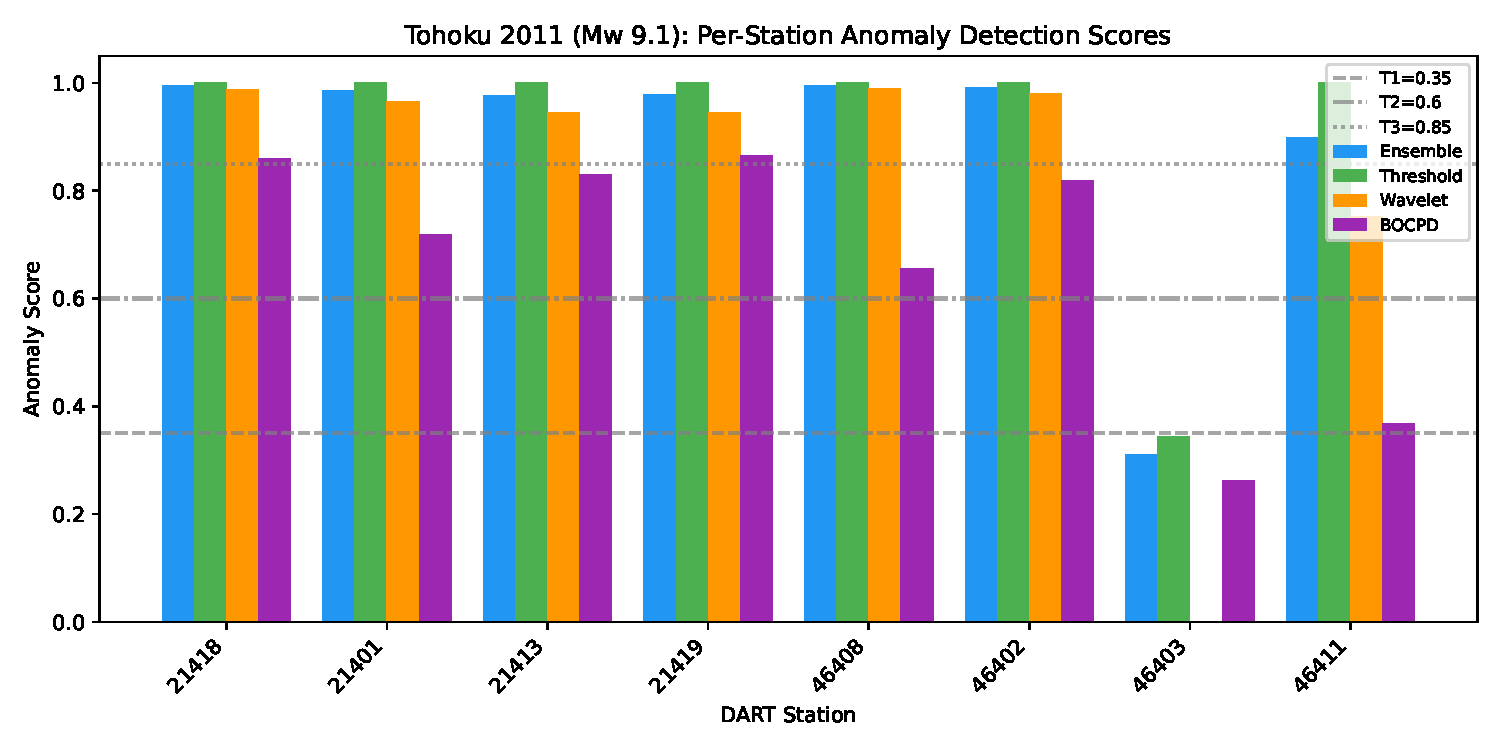
\includegraphics[width=\linewidth]{figures/fig5_tohoku_detection.pdf}
\caption{Tohoku 2011 per-station anomaly scores. Horizontal lines
  indicate FSM thresholds $T_1$, $T_2$, $T_3$. Generated by
  \texttt{scripts/generate\_paper\_figures.py} from
  \texttt{results/tohoku\_detection.json}.}
\label{fig:tohoku-detection}
\end{figure}

\begin{figure}[!htbp]
\centering
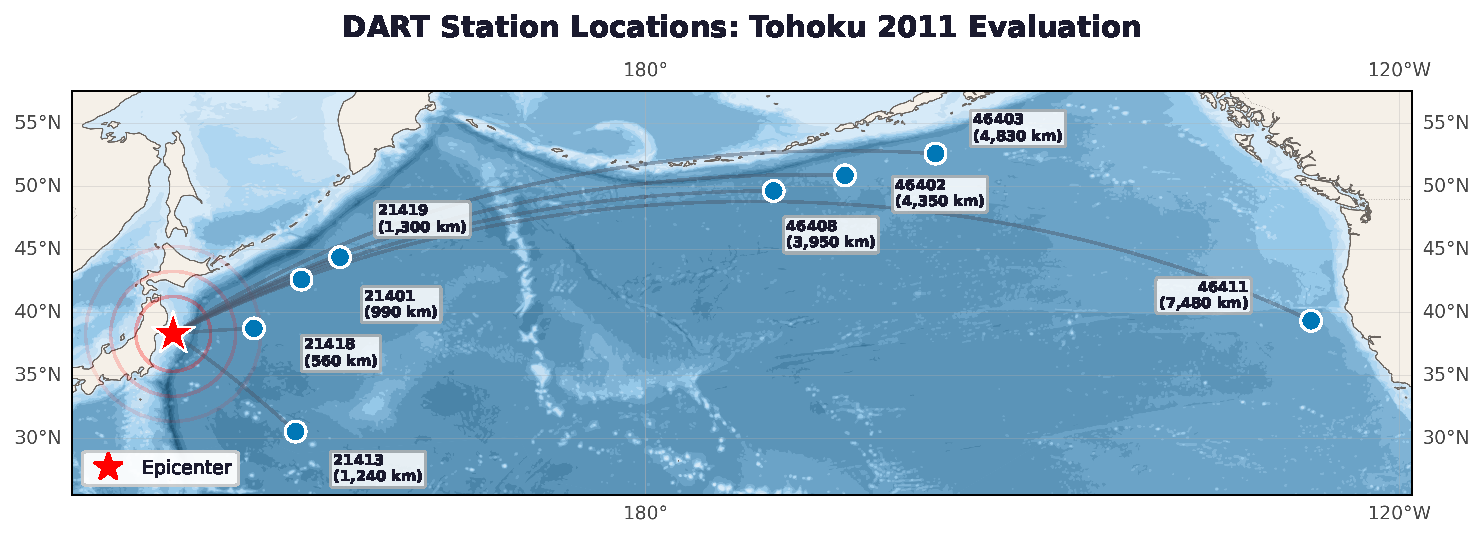
\includegraphics[width=\linewidth]{figures/fig_station_map.pdf}
\caption{DART station locations used for Tohoku 2011
  evaluation, with epicenter (red star) and epicentral
  distances.}
\label{fig:station-map}
\end{figure}

\begin{figure}[!htbp]
\centering
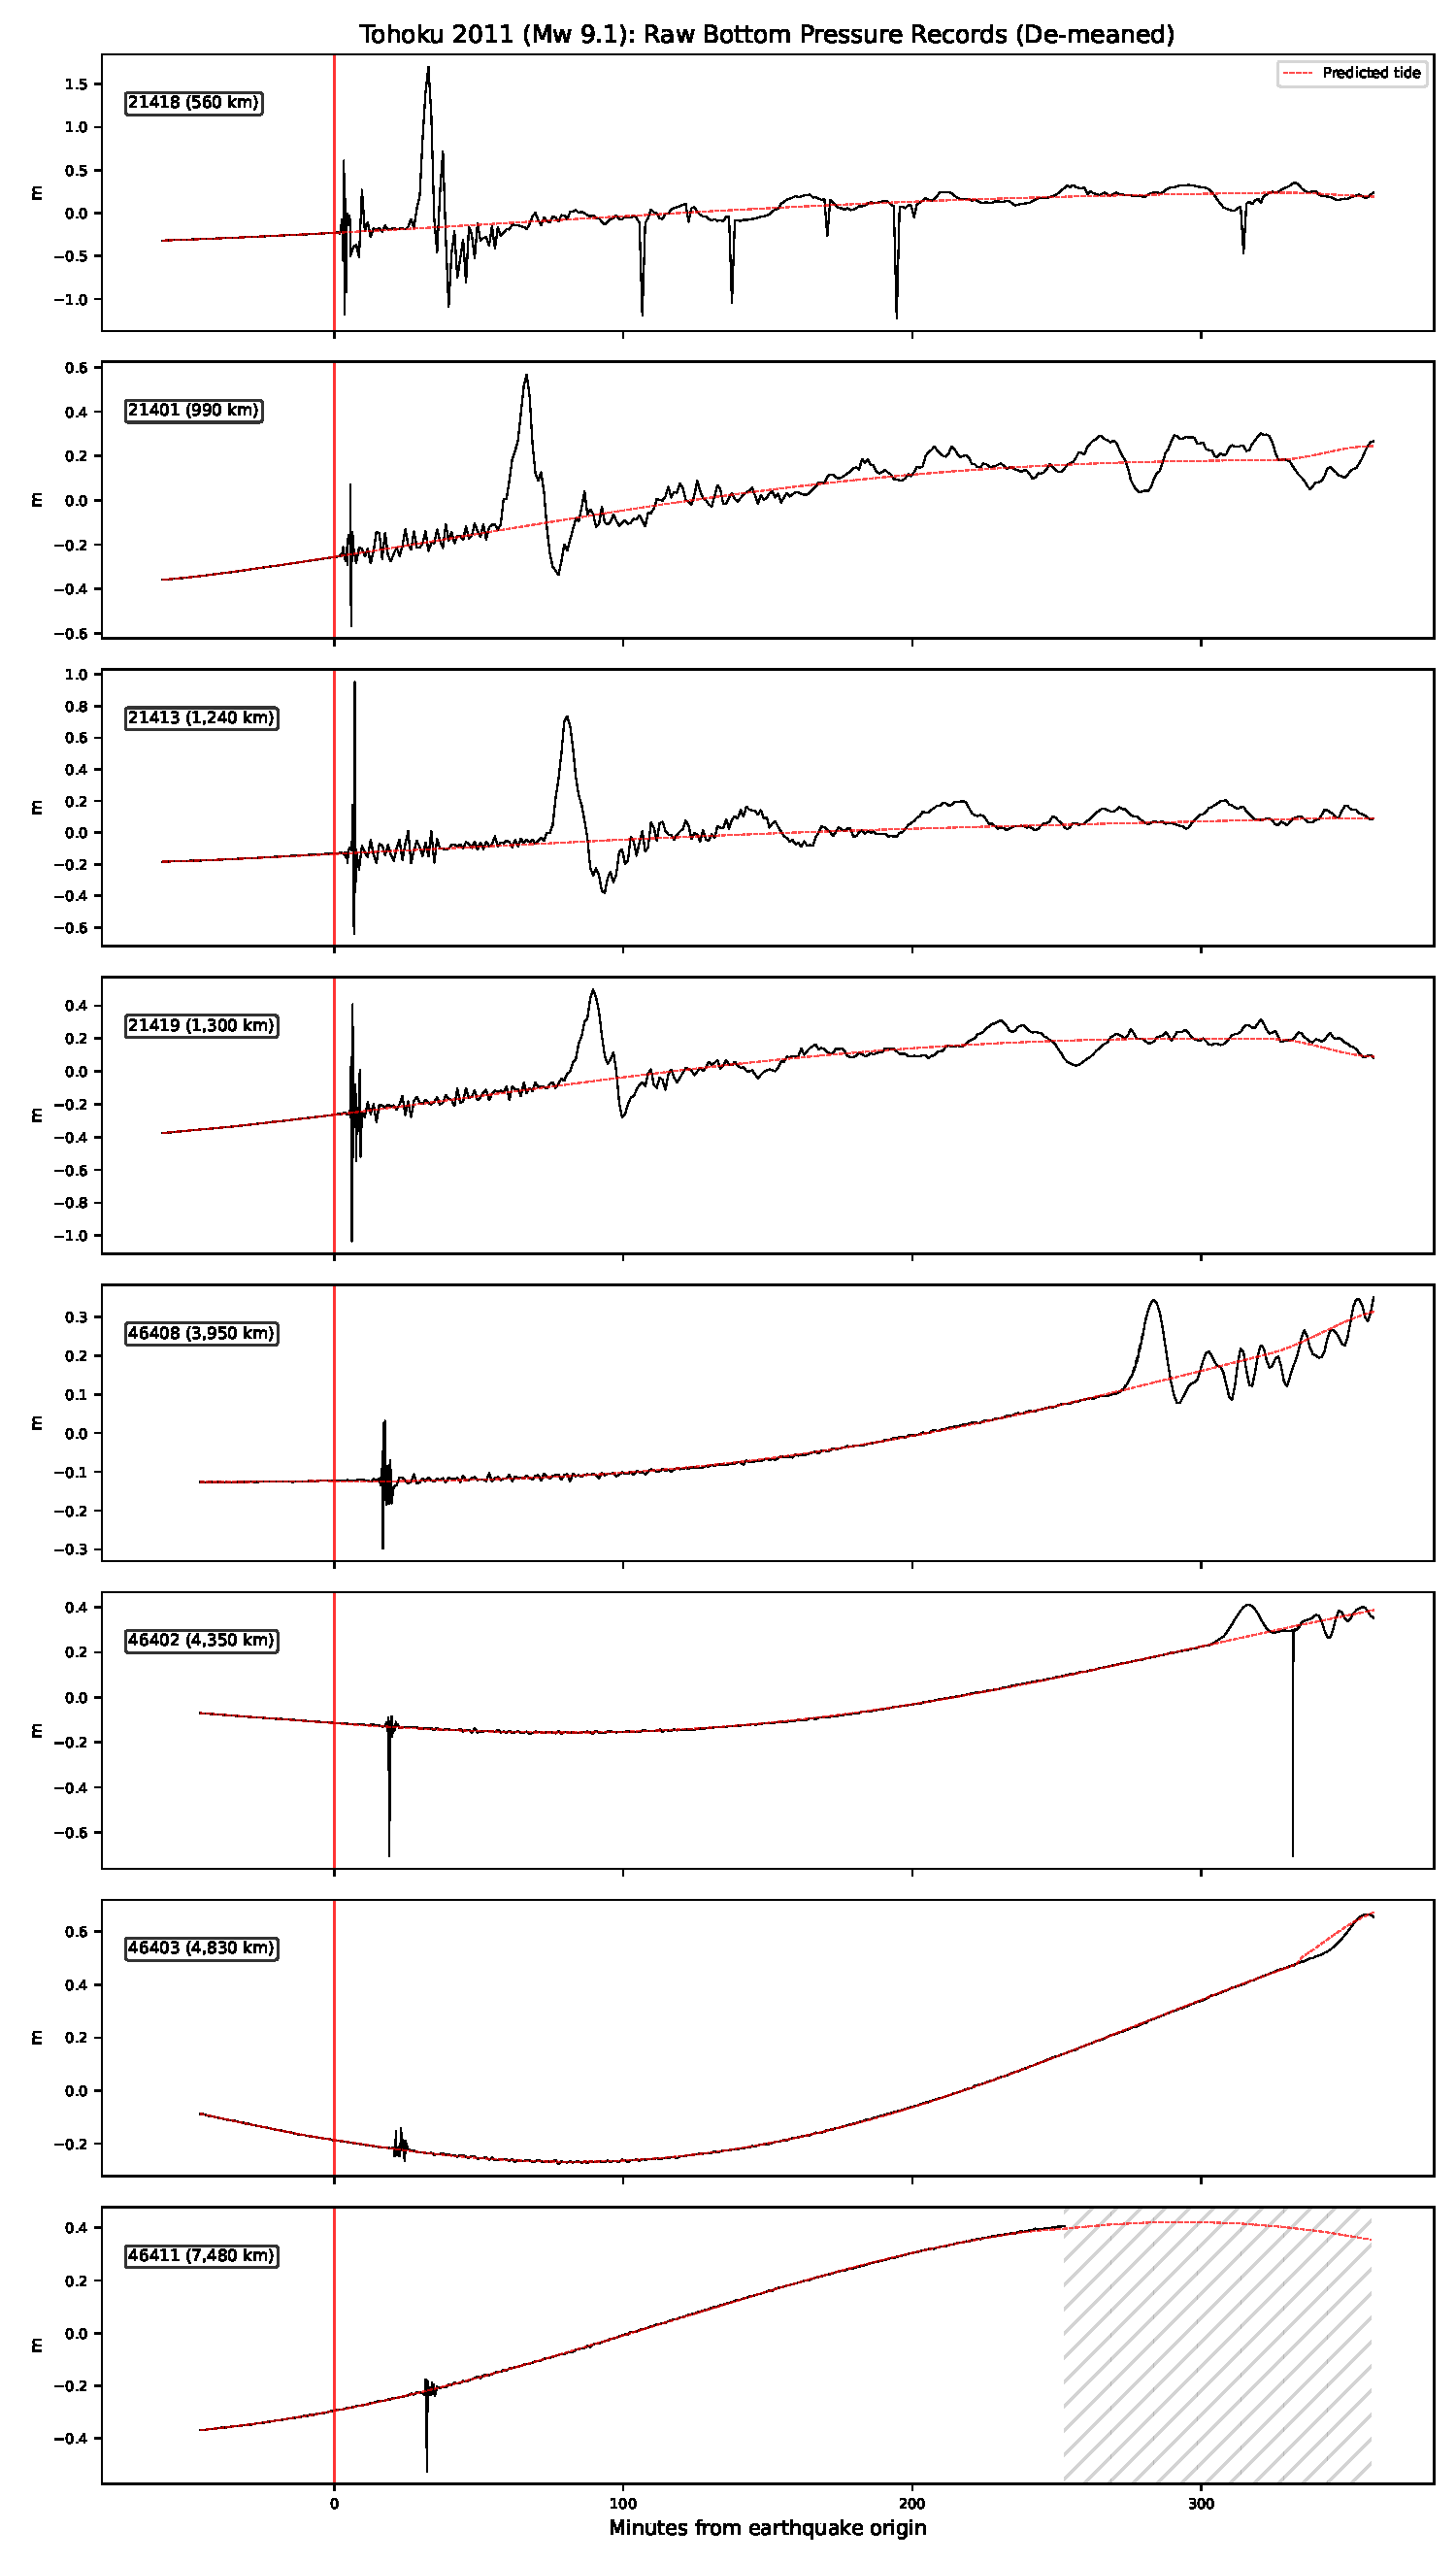
\includegraphics[width=0.82\linewidth]{figures/fig_tohoku_waveforms.pdf}
\caption{Tohoku 2011 raw bottom pressure records (de-meaned) for
  eight DART stations ordered by epicentral distance.  Red vertical
  line marks earthquake origin (05:46:24 UTC).  Pressure perturbations
  from seismic waves arrive within minutes at all stations.
  Longer-period tsunami oscillations are visible at the four
  near-field stations (21418, 21401, 21413, 21419; all
  $\le$1{,}300\,km).  At 3{,}950\,km, station~46408 may
  capture early tsunami energy near the end of the six-hour
  record; the three more distant stations show only seismic
  perturbations within this window.
  Red dashed curve: IRLS 8-constituent tidal prediction from 30-day
  calibration data.
  Hatched regions indicate data gaps.}
\label{fig:tohoku-waveforms}
\end{figure}

\begin{figure}[!htbp]
\centering
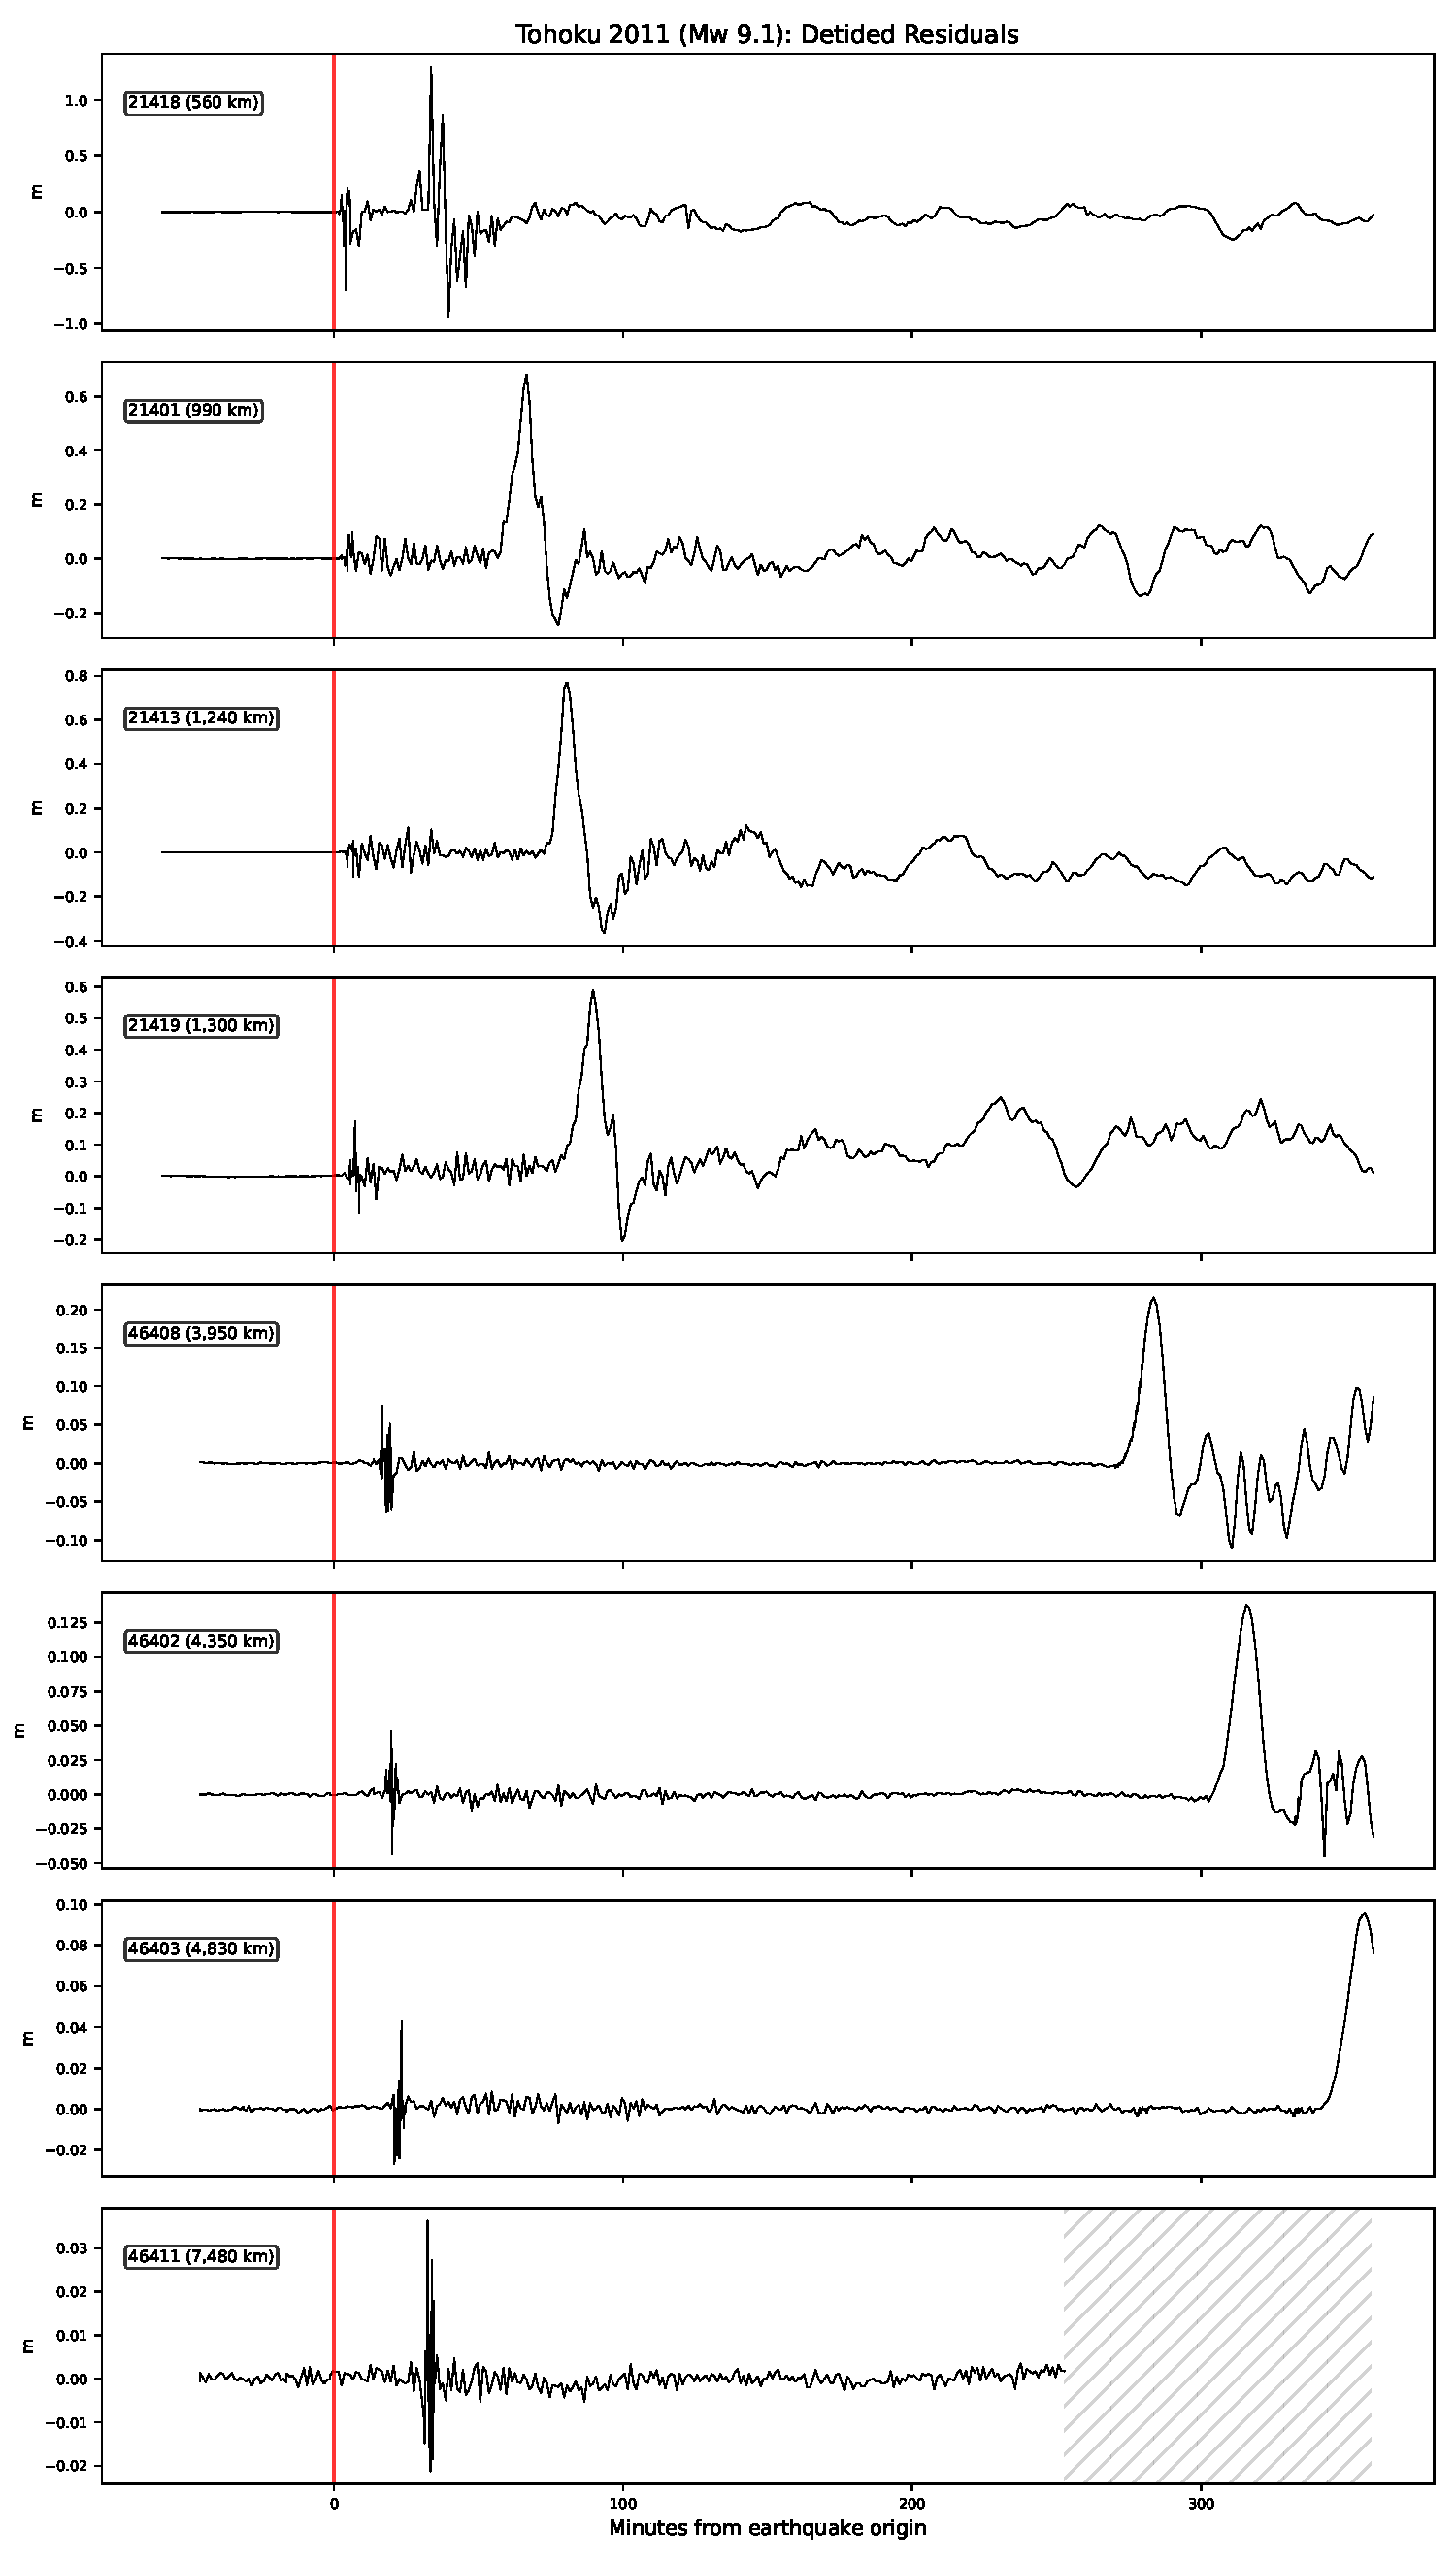
\includegraphics[width=0.82\linewidth]{figures/fig_tohoku_residuals.pdf}
\caption{Detided residuals (tsunami waveform) after removing
  the 8-constituent harmonic tidal prediction fitted on 30-day
  calibration data.  The isolated tsunami signal shows amplitude
  attenuation with distance.  Processing: level-shift correction,
  pre-event linear detrend, a 120\,min centered rolling median for
  stations beyond 3{,}000\,km to remove residual tidal curvature, and
  a Hampel spike filter.  This figure shows the detided residual
  before the bandpass; the filtered signal the detectors see appears
  in Figure~\ref{fig:score-overlay}.}
\label{fig:tohoku-residuals}
\end{figure}

\begin{figure}[!htbp]
\centering
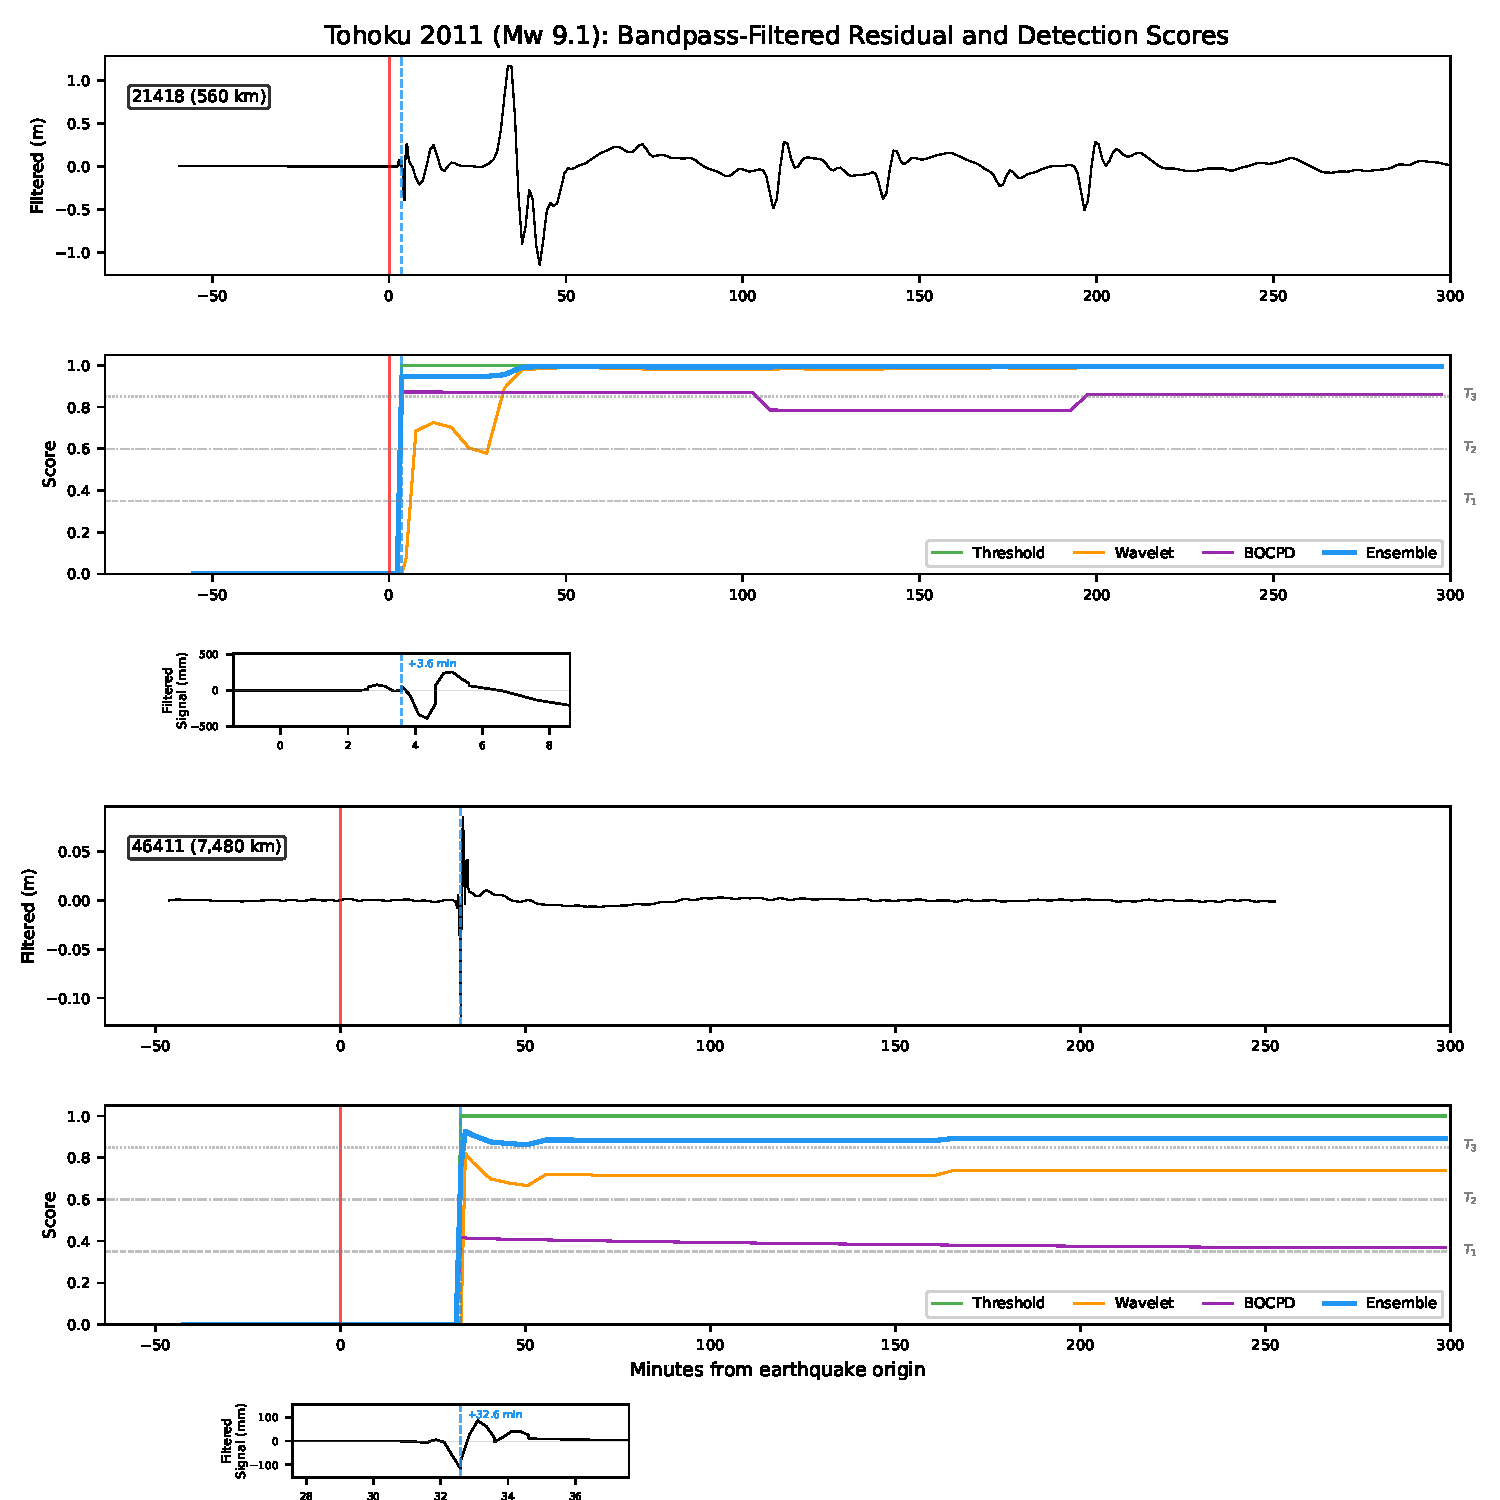
\includegraphics[width=\linewidth]{figures/fig_score_waveform_overlay.pdf}
\caption{Detection pipeline signals and scores for near-field
  station 21418 (560\,km) and far-field station 46411 (7{,}480\,km).
  For each station: (top) bandpass-filtered detided residual
  (5--120\,min passband, causal 4th-order Butterworth), identical to
  the signal processed by the threshold and wavelet detectors;
  (bottom) component and ensemble scores from sliding-window analysis
  with FSM thresholds $T_1$, $T_2$, $T_3$.
  The inset below each score panel shows the signal at mm scale
  around the score onset, the first nonzero ensemble score
  (blue dashed line).
  Scores simulate real-time processing: each window is a growing slice
  from the event start.
  At 46411 the ensemble score first becomes nonzero at
  ${+}32.6$\,min, coincident with the seismic Rayleigh wave, whose
  predicted arrival at 3.6\,km/s over 7{,}480\,km is 34.6\,min.  The
  detector responds to that surface-wave excursion, not to the
  tsunami, which is why the far-field score rises long before any
  water-level signal could have propagated this far.  The inset spans
  the onset $\pm$5\,min and shows the same excursion at mm scale.}
\label{fig:score-overlay}
\end{figure}


\subsection{Additional Case Studies}
\label{sec:eval-additional}

Four additional retrospective events are evaluated using the identical
pipeline configuration.  Full per-station results, waveform figures,
and agentic pipeline traces are provided in
Appendix~\ref{sec:appendix-case-studies}:
Chile 2010 ($M_w$\,8.8, \S\ref{sec:eval-chile}),
Illapel 2015 ($M_w$\,8.3, \S\ref{sec:eval-illapel}),
Iquique 2014 ($M_w$\,8.2, \S\ref{sec:eval-iquique}), and
Samoa 2009 ($M_w$\,8.1, \S\ref{sec:eval-samoa}).
Table~\ref{tab:cross-event-summary} consolidates detection rates
across all five events.

\noindent\textbf{Five-event summary.}
Across all five retrospective case studies
(T\={o}hoku 2011 $M_w$\,9.1, Chile 2010 $M_w$\,8.8, Illapel 2015
$M_w$\,8.3, Iquique 2014 $M_w$\,8.2, Samoa 2009 $M_w$\,8.1),
the ensemble detector triggers at event-mode DART stations within
$\sim$3{,}000\,km of the epicenter across a magnitude range of
$M_w$\,8.1--9.1.  The Samoa event further demonstrates that the
detector generalizes beyond subduction-zone thrust earthquakes to
outer-rise normal-faulting events.
Detection at greater distances uniformly requires event-mode switching
(1-min or 15-sec sampling) to resolve the tsunami energy band.

\FloatBarrier
\subsection{Detiding Validation}
\label{sec:eval-detiding}

Anomaly detection quality depends critically on tidal removal accuracy.
We validate the 8-constituent harmonic fit (Eq.~\ref{eq:tidal}) on 30~days of calibration data
per station (\texttt{scripts/validate\_detiding.py}).
For each station, we report the full-fit residual RMS, a holdout RMS
(fit on first 80\%, predict last 20\%), and extracted M2 and S2
constituent amplitudes (Figure~\ref{fig:detiding}).
Deep-ocean BPR M2 amplitudes in the range 0.1--1.0\,m are expected;
values outside this range indicate data quality issues.

After filtering NDBC 9999.000\,m missing-data sentinels, all eight
stations show realistic M2 amplitudes (0.11--0.65\,m).
Five stations achieve residual RMS of 0.04--0.09\,m; the remaining
three (21401, 21419, 21418) show elevated residuals of 0.14--0.36\,m,
likely due to non-tidal oceanographic signals (e.g., mesoscale eddies,
infragravity waves) that the 8-constituent harmonic model cannot capture.
Holdout RMS (fit on first 80\%, predict last 20\%) is below 0.10\,m
for six stations; stations 46403 and 21418 exhibit holdout RMS of
0.35--0.38\,m, indicating that the harmonic fit does not fully
generalize at those locations.
Sentinel filtering is applied at data retrieval, so the archived
CSVs used here are already clean; in initial processing of the raw
NDBC archive without this filter, five stations exhibited
catastrophically inflated M2 amplitudes (13--71\,m) because the
9999\,m outliers (deviating $\sim$4{,}000$\times$ from the tidal
signal) dominated the initial least-squares fit (a development
observation on the raw feed, not reproducible from the filtered
archive shipped with the repository).
The holdout RMS measures out-of-sample tidal prediction accuracy,
ensuring that the harmonic model generalizes beyond the fitting window.

DART bottom pressure recorders exhibit exponential and linear pressure
drift~\citep{watts1990drift}; a large fraction of total drift
occurs in the first days after deployment, with the rate depending on
instrument-specific time constants.  Our harmonic model includes only
a constant mean term $\bar{\eta}$, which absorbs a static offset but
\emph{cannot} absorb linear or exponential drift.  For the Tohoku 2011
stations (deployed months to years prior), drift rates are negligible
over the 30-day fitting window.  For recently deployed sensors, explicit
drift correction (e.g., subtracting a fitted exponential trend) should
precede harmonic analysis; this is not yet implemented.

\begin{figure}[!htbp]
\centering
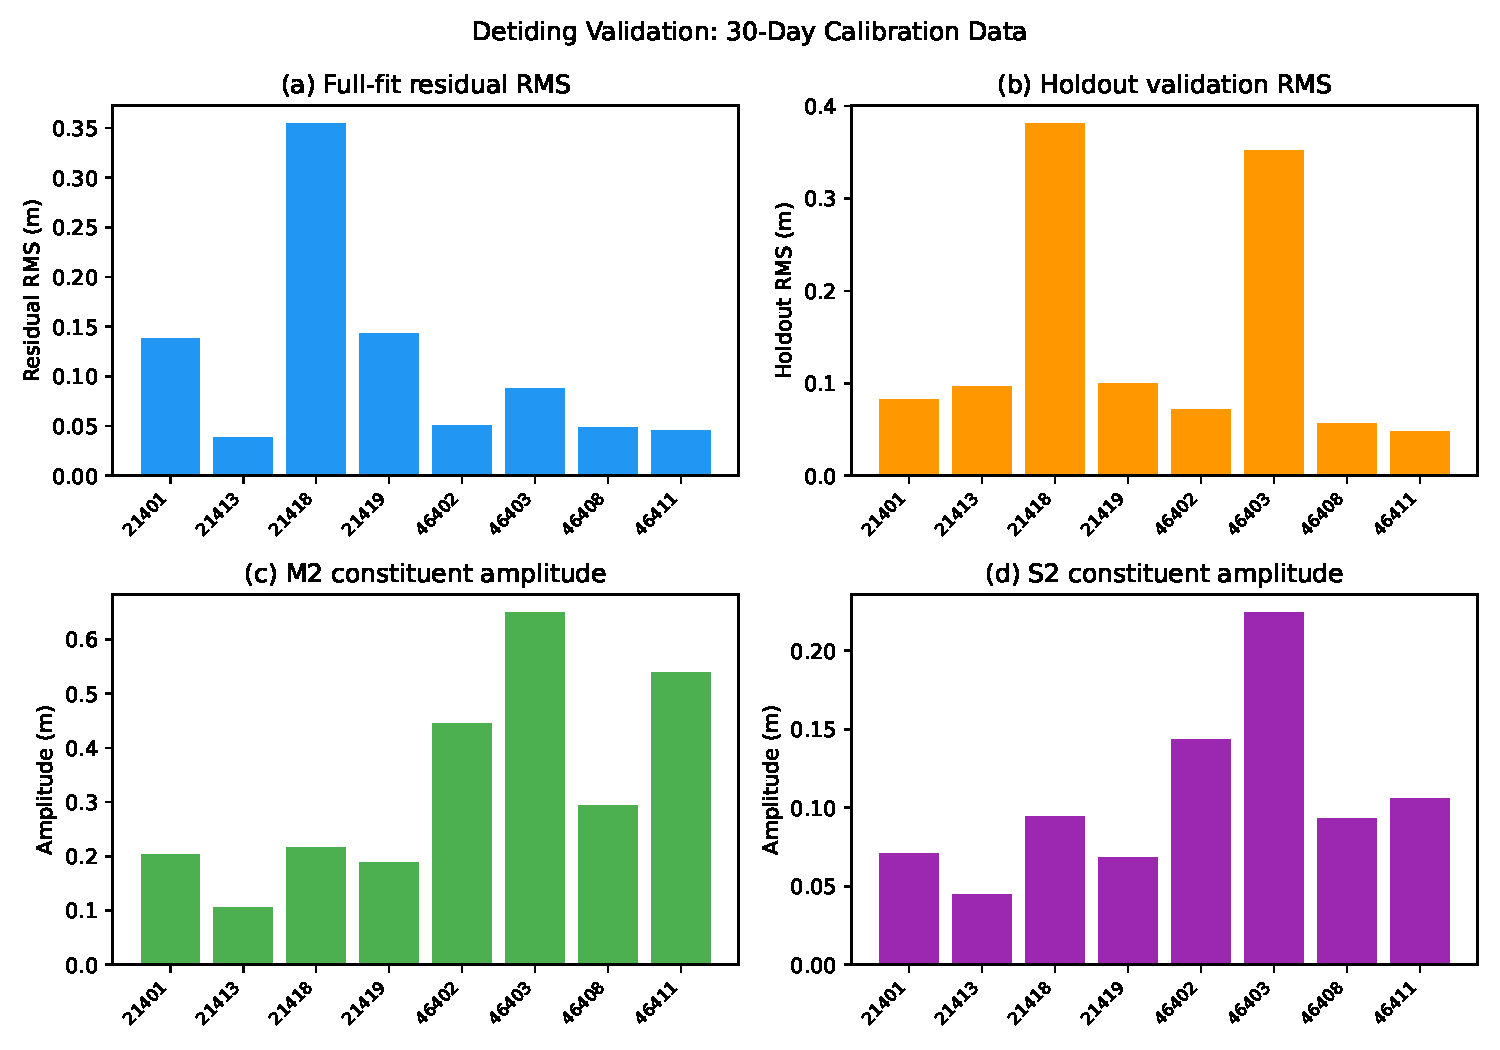
\includegraphics[width=\linewidth]{figures/fig6_detiding_quality.pdf}
\caption{Detiding validation on 30-day calibration data: (a)~full-fit
  residual RMS, (b)~holdout RMS, (c)~M2 amplitude, (d)~S2 amplitude
  per station. Generated from
  \texttt{results/detiding\_validation.json}.}
\label{fig:detiding}
\end{figure}

\FloatBarrier
\subsection{Component Score Decomposition}
\label{sec:eval-components}

The ensemble score (Eq.~\ref{eq:ensemble}; without ML, Eq.~\ref{eq:ensemble_noml}) combines a threshold
detector and the maximum of wavelet and BOCPD scores. To understand
which components drive detection, we decompose scores across the
sliding-window timeline for near-field and far-field stations
(Figure~\ref{fig:score-decomposition}).
By design, near-field stations receive higher-amplitude arrivals
that should activate both the threshold and wavelet detectors, while
far-field stations receive attenuated signals where the BOCPD detector
is expected to contribute more via distributional-shift detection in
the broadband residual (Figure~\ref{fig:score-decomposition}).

\begin{figure}[!htbp]
\centering
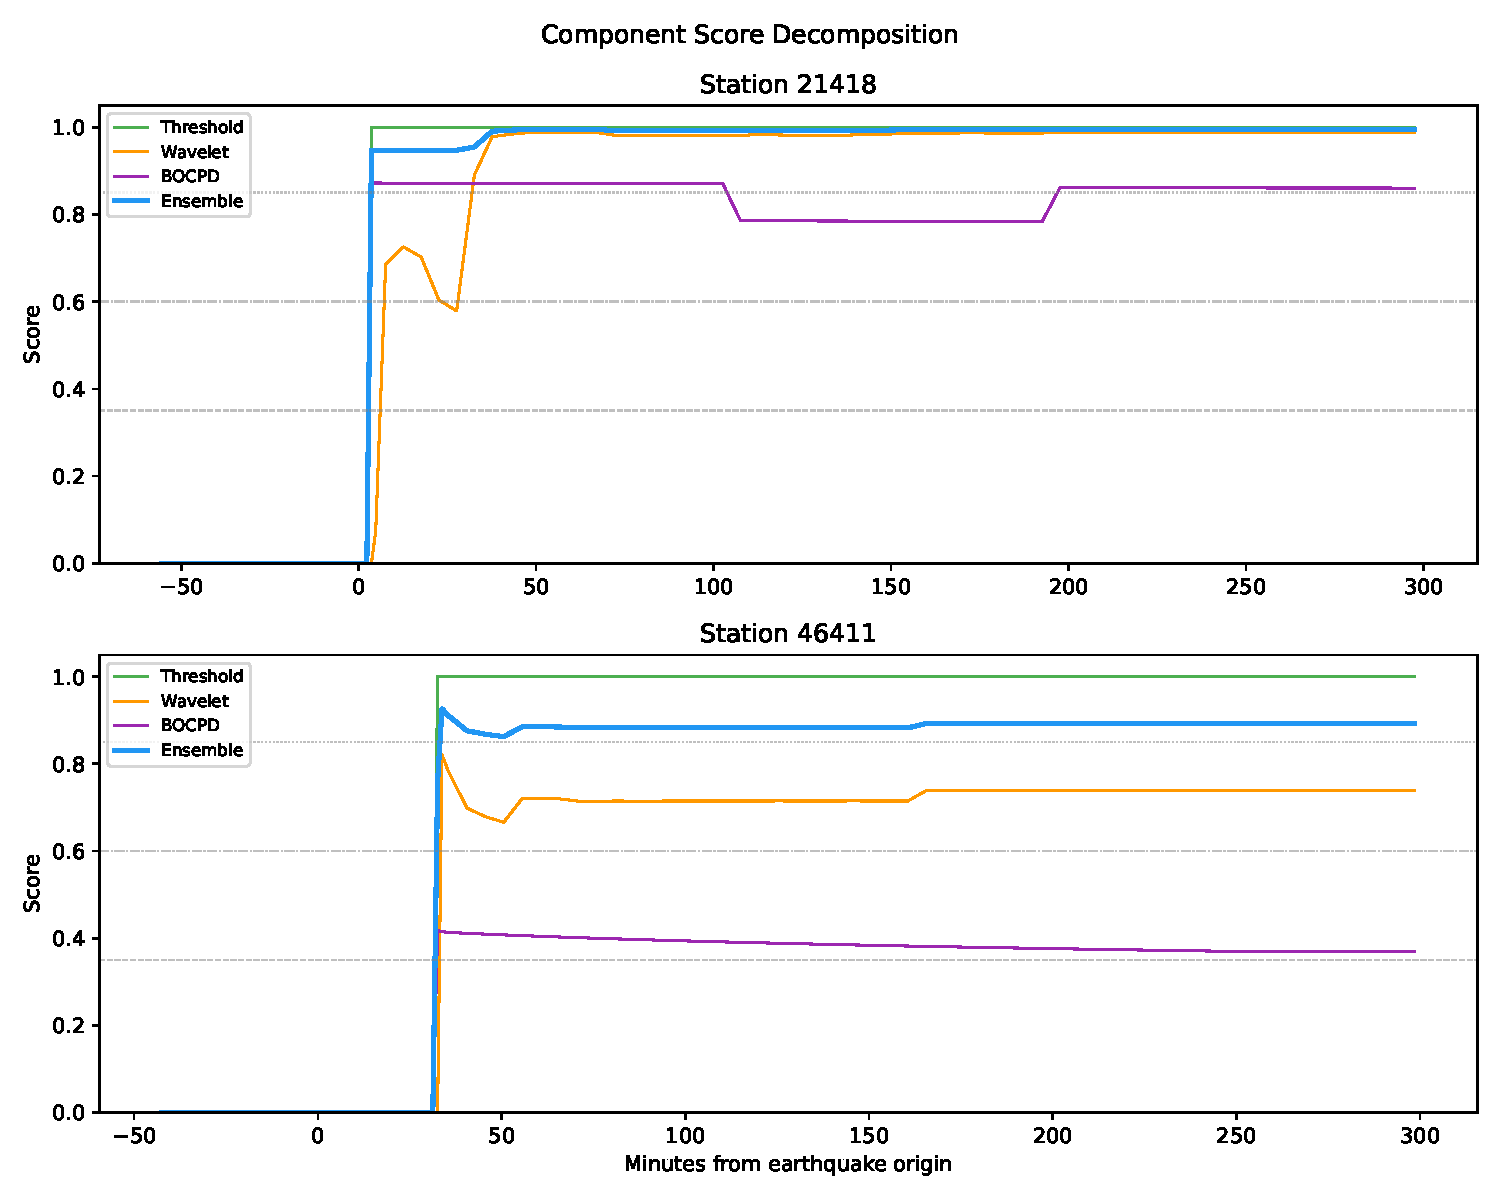
\includegraphics[width=\linewidth]{figures/fig7_score_decomposition.pdf}
\caption{Component score decomposition over time for selected
  stations. The ensemble score combines threshold (amplitude-based)
  and statistical (max of wavelet, BOCPD) detectors.}
\label{fig:score-decomposition}
\end{figure}

\FloatBarrier
\subsection{Component Ablation}
\label{sec:eval-ablation}

To quantify each detector's contribution to the ensemble, we recompute
per-station ensemble scores under four weight configurations using the
component scores from Section~\ref{sec:eval-components}
(\texttt{scripts/run\_ablation.py}).  Because the Isolation Forest is
not deployed, the last two configurations coincide and only three are
distinct; see the caption.
Table~\ref{tab:ablation} reports the number of stations crossing each
FSM threshold.

\begin{table}[!htb]
\centering
\caption{Ablation study: detection outcomes under four weight
  configurations, on T\={o}hoku 2011 (8 stations).  $\ge T_k$ counts
  stations whose ensemble score reaches threshold~$T_k$.  Weights are
  $(\alpha_{\text{thr}},\alpha_{\text{stat}},\alpha_{\text{ml}})$.
  The Isolation Forest is not deployed, so no ML score enters any
  configuration: in the last row $s_{\text{ml}}$ is absent, so the
  implementation renormalizes over the two remaining detectors to
  $(0.5882, 0.4118)$, the unrounded form of the weights printed in
  Eq.~\ref{eq:ensemble_noml}.  That makes it the Threshold+Stat row up to
  the rounding of the tabulated weights (per-station agreement to within
  $6\times10^{-5}$).  Only three detector configurations are
  therefore distinct, and $\alpha_{\text{ml}}$ is untested.}
\label{tab:ablation}
\small
\begin{tabular}{lcccc}
\toprule
\textbf{Configuration} & \textbf{Weights}
  & $\ge T_1$ & $\ge T_2$ & $\ge T_3$ \\
\midrule
Threshold-only & (1.0, 0.0, 0.0) & 7/8 & 7/8 & 7/8 \\
Statistical-only & (0.0, 1.0, 0.0) & 7/8 & 7/8 & 6/8 \\
Threshold+Stat & (0.588, 0.412, 0.0) & 7/8 & 7/8 & 7/8 \\
Full ensemble & (0.50, 0.35, 0.15) & 7/8 & 7/8 & 7/8 \\
\bottomrule
\end{tabular}
\end{table}

Every configuration detects 7/8 stations at $T_1$: station~46403
stays below threshold in all of them (its strongest channel, the
threshold detector, peaks at 0.344; its statistical score reaches
only 0.263 via BOCPD).
Statistical-only detection also does not reach $T_3$ at 46403 or
46411, indicating reduced discrimination at far-field distances,
while every configuration that includes the threshold detector
reaches $T_3$ at 7/8 stations.  On this event the threshold
detector is what carries detection; the statistical detector changes
no station's outcome.  One event of eight stations is too small to
generalize that split.

Sliding-window analysis shows identical earliest detection
times across configurations (3.6~min post-earthquake at station~21418),
because the dominant early signal is coseismic seafloor deformation
and long-period seismic energy (including surface waves), which
saturates the threshold detector.
A threshold sensitivity sweep over the full-record scores shows 7/8
at the operating $T_1 = 0.35$ (station 46403 stays below threshold);
lowering $T_1$ to 0.30 admits 46403's full-record score of 0.311, and
raising it to 0.45 still yields 7/8.  In the sliding replay, 46403's
ensemble peaks at 0.198, so no tested threshold detects it during the
event.
The earliest sliding-window detection time (3.6~min) is invariant to
$T_1$ across the sweep because the near-field seismic signal saturates
well above all tested thresholds.
Statistical validation of component weights across a broader event
catalog remains future work.

\FloatBarrier
\subsection{FSM Transition Latency}
\label{sec:eval-fsm}

Table~\ref{tab:fsm-transitions} reports the first time each station's
sliding-window ensemble score crosses the FSM thresholds $T_1$, $T_2$,
$T_3$ (\texttt{scripts/analyze\_fsm\_transitions.py}).

\begin{table}[!htb]
\centering
\caption{Detection latency: minutes from earthquake origin to first
  threshold crossing per station, ordered by distance.}
\label{tab:fsm-transitions}
\small
\begin{tabular}{lrccc}
\toprule
\textbf{Station} & \textbf{Dist (km)}
  & $T_1$ \textbf{(min)} & $T_2$ \textbf{(min)} & $T_3$ \textbf{(min)} \\
\midrule
21418 &   560 &  3.6 &  3.6 &  3.6 \\
21401 &   990 &  5.6 &  7.6 & 62.6 \\
21413 & 1{,}240 &  7.6 &  7.6 &  7.6 \\
21419 & 1{,}300 &  6.3 &  7.6 &  7.6 \\
46408 & 3{,}950 & 18.8 & 18.8 & 18.8 \\
46402 & 4{,}350 & 19.1 & 20.3 & 20.3 \\
46403 & 4{,}830 &  --- & --- & --- \\
46411 & 7{,}480 & 32.6 & 32.6 & 33.8 \\
\bottomrule
\end{tabular}
\end{table}

Near-field stations (21418, 21401, 21413, 21419; all $\le$1{,}300\,km) reach $T_1$ within
3.6--7.6~min, consistent with coseismic seafloor deformation and
long-period seismic energy entering the 5--120\,min passband.
Station~21401 shows a notable gap between $T_2$ (7.6~min) and $T_3$
(62.6~min): the early seismic signal crosses $T_2$ quickly, but
$T_3$ requires the larger-amplitude tsunami arrival.
Far-field stations 46408 and 46402 show $T_1$ crossings at 18.8 and
19.1~min, after the P-wave arrival at those distances
(${\sim}8$ and ${\sim}9$\,min at ${\sim}8$\,km/s) and consistent
with long-period surface-wave energy at Rayleigh group velocities
(3{,}950\,km in 18.8\,min and 4{,}350\,km in 19.1\,min imply
3.5 and 3.8\,km/s).
Station~46411 reaches $T_1$ at 32.6~min, an implied group velocity
of 3.8\,km/s at 7{,}480\,km, consistent with the same surface-wave
arrival.
Station~46403 does not cross $T_1$ at all: the sliding-window
timeline peaks at an ensemble score of~0.198 and the full 6-hour
window yields ensemble~$= 0.311$ (Table~\ref{tab:tohoku-results});
the signal is marginal at this distance (4{,}830\,km).

\FloatBarrier
\subsection{Quiet-Period False Trigger Analysis}
\label{sec:eval-false-positive}

To measure the false positive rate, we process 30~days of quiet-period
DART data (June 2011, no significant tsunamis) for the same eight
stations (\texttt{scripts/run\_false\_positive\_evaluation.py}).
The first 15~days serve as calibration; the remaining 15 days
are processed in non-overlapping 6-hour windows with no seismic
context. The metric is the number of windows where the ensemble score
exceeds $T_1 = 0.35$ (false INVESTIGATE triggers) per station-month.

Note that the quiet-period data uses 15-minute standard-mode sampling,
which triggers the \texttt{filter\_degraded} flag (the bandpass Nyquist
criterion needs sampling faster than 150\,s; at exactly 150\,s the
filter is already degraded).  In degraded mode the
passband upper edge is clamped to Nyquist, giving roughly a 30 to
120\,min passband rather than 5 to 120\,min.  The threshold and
wavelet scores are not suppressed by this: they are computed on the
clamped and partly aliased output and should be read as unreliable in
either direction rather than as absent.  The rates measured here are
therefore not a clean measurement of any single detector, and not the
full ensemble operating in event mode (1-minute sampling).

Across 7 evaluated stations (station 46402 had insufficient June 2011
data), we observe 1 window exceeding $T_1$ and $T_2$ (station~46408,
max score 0.80) and zero windows exceeding $T_3$ across 414 total
windows (15 evaluation days per station; two stations yielded fewer
than the full 60 windows because of data gaps, 55 at 46403 and 59 at
46408).  This corresponds to
${\sim}0.29$ false $T_1$ triggers per station-month.  The single
false trigger is driven by a threshold-score spike from a
large-amplitude isolated pressure transient at the 46408 BPR that
exceeded the detection threshold even in degraded mode (the bandpass
filter's attenuation is less effective against impulsive transients
than against periodic signals).  Re-running that window with
component logging gives a saturated threshold score of 1.00, a
wavelet score of 0.52, and a BOCPD score of 0.00, which reproduce the
0.80 ensemble under Eq.~\ref{eq:ensemble_noml}.  The
threshold detector therefore supplies 0.59 of the 0.80, and the
wavelet detector responds to the same transient rather than firing
independently; BOCPD alone stays silent.  An event-mode (1-minute sampling)
quiet-period evaluation using non-tsunamigenic seismic events would
test the full ensemble and is planned as future work.

\FloatBarrier
\subsection{Synthetic Detection Sensitivity}
\label{sec:eval-synthetic}

We characterize the minimum detectable signal using synthetic
tidal-plus-noise signals with injected tsunami waveforms at varying
amplitudes and periods
(\texttt{scripts/run\_synthetic\_evaluation.py}).
The evaluation grid spans amplitudes from 0.005 to 0.50\,m,
periods from 5 to 120\,min, noise levels of 0.0005--0.005\,m,
and sampling intervals of 15\,s and 60\,s.

For each configuration, we record the maximum FSM state reached
(MONITOR, INVESTIGATE, ASSESS, or ESCALATE) at the system's
fixed operating points. Figure~\ref{fig:synthetic-heatmap} shows
the resulting sensitivity heatmap for the representative
configuration (noise = 0.001\,m, sampling = 60\,s).
This is \emph{not} a ROC curve: the thresholds are fixed design
constants, and we evaluate detection at those operating points rather
than sweeping a decision boundary.

\begin{figure}[!htbp]
\centering
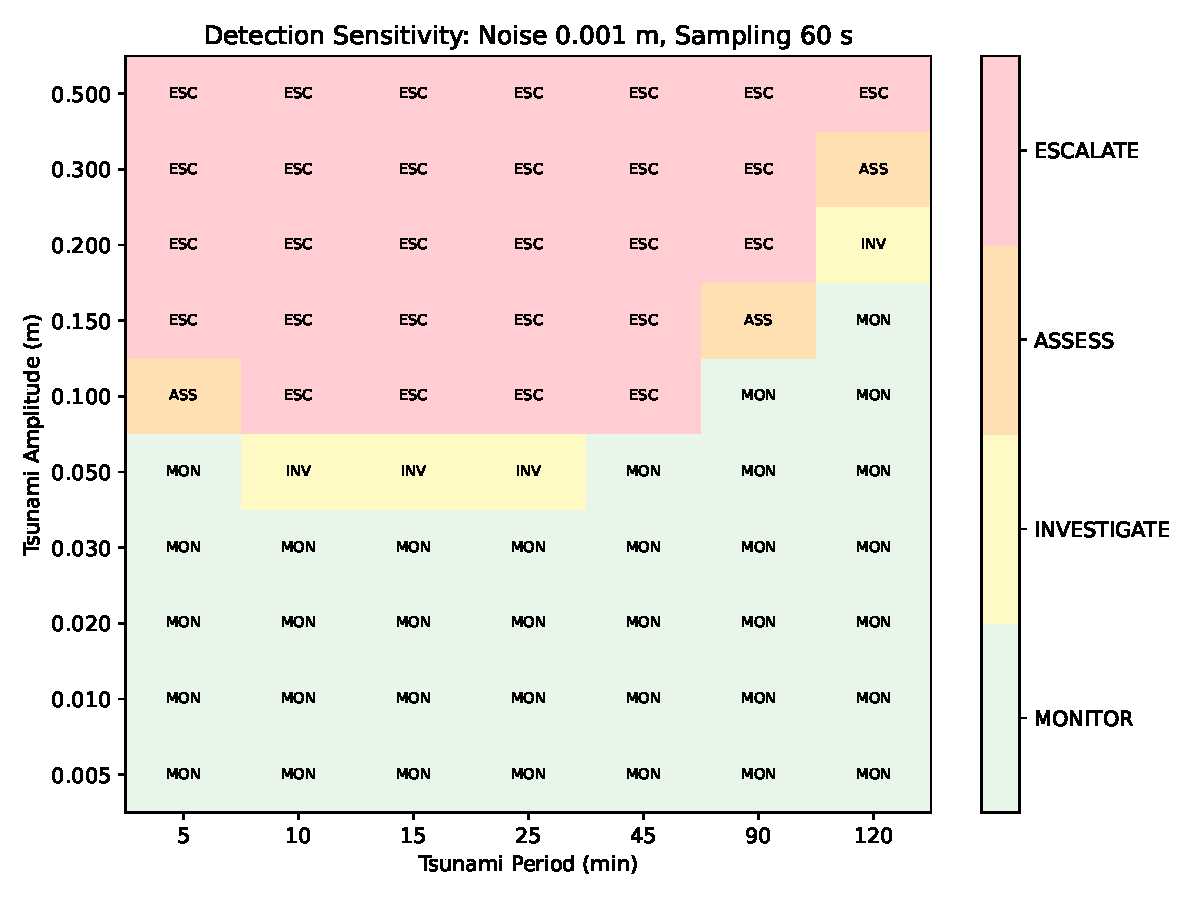
\includegraphics[width=0.9\linewidth]{figures/fig8_synthetic_heatmap.pdf}
\caption{Synthetic detection sensitivity heatmap (noise = 0.001\,m,
  sampling = 60\,s). Each cell shows the maximum FSM state reached
  for a given (amplitude, period) configuration.
  The ASSESS state ($T_2 \le s < T_3$) rarely appears because signals
  strong enough to cross $T_2$ typically also cross $T_3$ within the
  analysis window, producing a sharp INVESTIGATE-to-ESCALATE boundary.}
\label{fig:synthetic-heatmap}
\end{figure}

\FloatBarrier
\subsection{ABSTAIN Correctness}
\label{sec:eval-abstain}

The verification layer (\S\ref{sec:verification}) enforces
conservative degradation when observational data are insufficient.
A check whose input is absent does not return a trivial PASS.  It
returns NOT\_EVALUATED with its prerequisite marked MISSING, so only
checks that actually ran on available data can PASS.  The aggregate
follows from the applicability the constraint stage assigns each
check: any FAIL gives FAIL; a REQUIRED check whose prerequisite is
MISSING or ERROR gives INCOMPLETE; a CONCERN, or an OPTIONAL check
without its prerequisite, gives PASS\_WITH\_CONCERNS.  FAIL and
INCOMPLETE both set \texttt{abstain\_required} and route to ABSTAIN,
so insufficient data reaches the same safety path as contradicted
data.  A stage at which no check applies at all is itself INCOMPLETE,
which closes the case where an empty evidence base could otherwise
look like agreement.  PASS is the residual outcome, reached only when
every applicable check ran and returned PASS.  The station-count
safeguard that bears on this outcome is the verification layer's DART
coverage check, which returns FAIL below two contributing stations; the
spatial coherence score of \S\ref{sec:anomaly} does not, since it
reaches only the unloaded Isolation Forest.
The absent-input path is covered by tests such as
\texttt{test\_no\_holdout\_is\_not\_evaluated}, alongside the
aggregation tests over \texttt{determine\_outcome}.

\FloatBarrier
\subsection{Pipeline Latency}
\label{sec:eval-latency}

Table~\ref{tab:latency} reports measured latencies from
\texttt{scripts/profile\_latency.py} (50 iterations, Apple M-series
laptop). The anomaly detection pipeline (detiding, bandpass filtering,
wavelet analysis, BOCPD, and ensemble fusion) completes in
$\sim$47\,ms at p95, dominated
by the BOCPD computation ($\sim$44\,ms). QC checks process 10 records
in ${\sim}0.12$\,ms, and FSM transitions are sub-millisecond. The
computational cost of the signal processing pipeline is well within
real-time requirements for 1-minute DART event-mode data.

\FloatBarrier
\subsection{Synthetic Scenario Verification}
\label{sec:eval-physics-sim}

To verify the system's end-to-end behavior under controlled conditions
beyond the five historical case studies, we evaluate four synthetic
scenarios generated by a deterministic simulation framework
(\texttt{scripts/run\_physics\_validation.py}).  Each scenario injects
multi-frequency waveforms at multiple stations with source amplitudes
using the Comer~\citep{comer1980tsunami} non-dispersive scaling slope
(0.75; intercept calibrated to approximate observed DART amplitudes),
deep-ocean propagation at
$\sqrt{g \cdot 4000}\approx 198$\,m/s, geometric spreading
($A \propto 1/\sqrt{r}$), and (for coastal stations) Green's Law
shoaling amplification ($A_\text{shore}/A_\text{deep} =
(h_\text{deep}/h_\text{shore})^{1/4}$).
These scenarios constitute a \emph{verification} exercise, not an
independent validation: the simulator and detector share the same tidal
constituent set, wave speed constant, and noise model assumptions.
They test whether the software correctly propagates signals through
the pipeline and whether the FSM transitions fire at the designed
thresholds.  The retrospective evaluations on real Tohoku and Chile
DART records (\S\ref{sec:eval-tohoku}; additional events in Appendix~\ref{sec:appendix-case-studies})
provide the scientifically independent validation against observed data.

\paragraph{Scenario~1: Large tsunami (M8.5 Aleutian).}
A simulated $M_w$\,8.5 thrust earthquake at 25\,km depth on the
Aleutian arc (52.5\textdegree N, 173.0\textdegree W) triggers the
FSM via a synthetic USGS FDSN event notification.
Nine stations (6~DART, 3~CO-OPS) spanning 2{,}448--3{,}960\,km from
the epicenter receive synthetic waveforms.
All nine stations exceed $T_1$ and $T_2$; the three CO-OPS stations
also exceed $T_3$ (ensemble scores 0.91--0.94), while DART stations reach
ensemble scores of 0.69--0.73 (Figure~\ref{fig:physics-scenario1}).
The higher CO-OPS scores reflect Green's Law coastal amplification:
characteristic tsunami amplitudes of 0.23--0.28\,m at the shallow-water
stations (10--20\,m depth) versus 0.025--0.032\,m at the deep-ocean DART
BPRs.  Throughout this section an amplitude quoted for a synthetic station
is the source model's characteristic amplitude carried to that station by
geometric spreading, directivity and any coastal factor.  It is not the peak
of the simulated record: the synthesized waveform sums many spectral
components, so its excursion runs a few times larger.
The Aleutian epicenter is roughly equidistant from the NW~Pacific and
NE~Pacific station clusters, producing arrival times (3.4--5.6\,hr)
distinct from the Tohoku validation event, showing that
detection does not depend on a specific source location.

\paragraph{Scenario~2: Moderate earthquake (M7.0 Aleutian).}
Four DART stations: all ensemble scores remain below $T_1 = 0.35$,
confirming no false escalation for sub-tsunamigenic events with
characteristic deep-ocean amplitudes of ${\sim}0.009$\,m.

\paragraph{Scenario~3: Meteotsunami false positive.}
A 0.10\,m, 20-minute period meteotsunami injected at a single CO-OPS
station with no seismic activity.  The ensemble score is zero:
the 0.10\,m amplitude falls below the CO-OPS detection threshold
(0.15\,m), producing a threshold score of zero independently of
other factors.  The seismic quiet penalty (which raises the effective
detection threshold by 30\% when no $M \geq 6.5$ earthquake is
reported within 90 minutes) provides an additional suppression layer
but is not the primary rejection mechanism in this scenario.
The rejection should therefore be read as conditional on that
threshold, which is a screening default rather than a calibrated
figure, and the margin is not large: the injection sits a third below
the 0.15\,m level, and it is that level rather than the quiet-period
penalty that rejects it.  The operational levels are higher again,
with NWSI 10-701 Section 3.4 reserving an Advisory for a forecast of
0.3 to 1.0\,m and canceling products once height falls below
0.3\,m~\citep{nwsi10701}.

\paragraph{Scenario~4: Partial network outage.}
Four of six DART stations offline.  Both remaining online stations
(21418 and 21419) detect the
tsunami signal, so detection survives the outage: each station is scored
independently and neither crossing depends on the others.  Two stations
is also the floor the verification layer's DART coverage check enforces,
below which it returns FAIL.

Figure~\ref{fig:physics-summary} presents the four-scenario summary.
Together, these scenarios verify correct detection across distance
ranges, false positive rejection (sub-threshold amplitude, with the
seismic quiet penalty adding margin), and
continued operation under partial network failure.

\begin{figure}[!htbp]
\centering
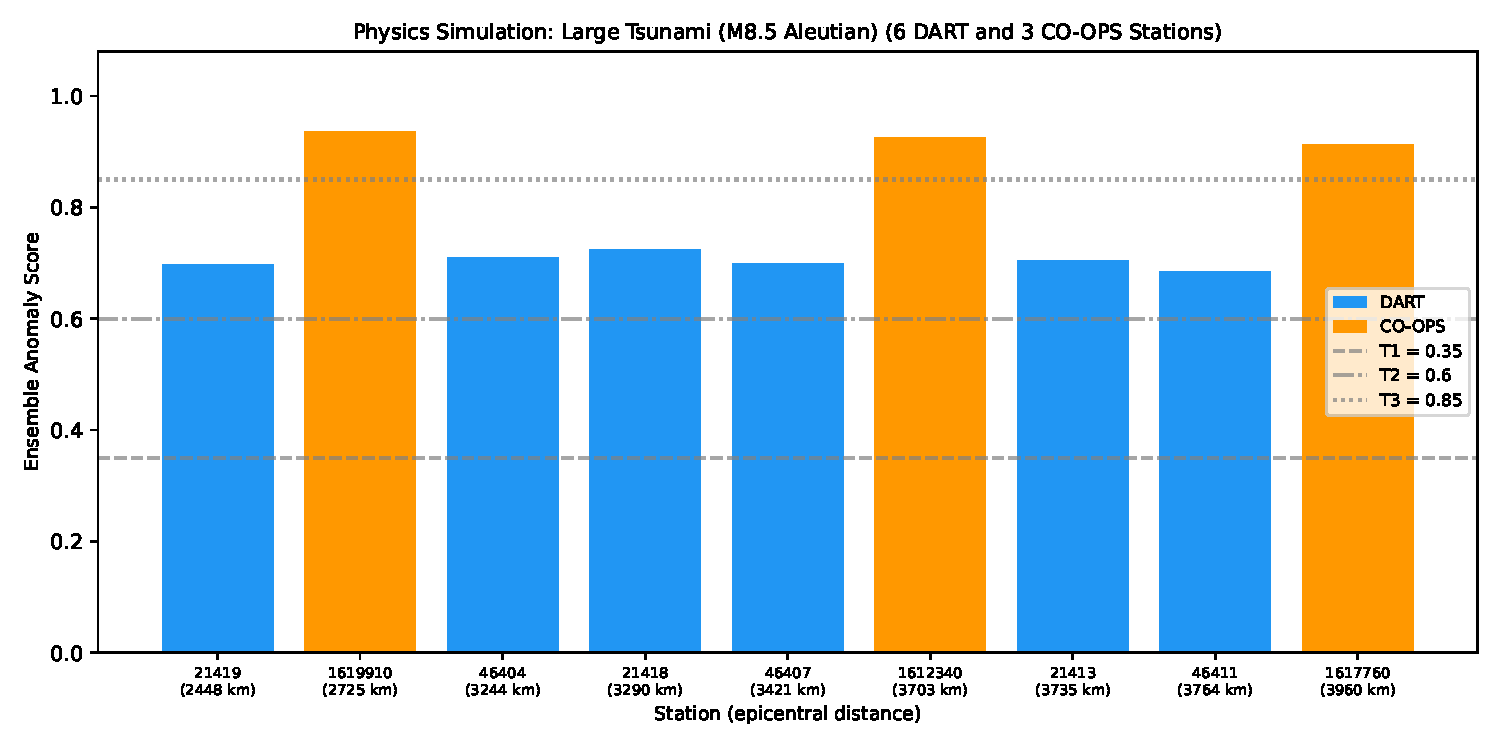
\includegraphics[width=\linewidth]{figures/fig_physics_scenario1.pdf}
\caption{Physics simulation Scenario~1 (M8.5 Aleutian): per-station
  ensemble anomaly scores.  Blue bars: DART stations; orange bars:
  CO-OPS stations.  Horizontal lines show FSM thresholds $T_1$, $T_2$,
  $T_3$.  Station labels include epicentral distance.  All stations
  exceed $T_2$; the three CO-OPS stations also cross $T_3$ due to
  Green's Law coastal amplification of the tsunami signal.}
\label{fig:physics-scenario1}
\end{figure}

\begin{figure}[!htbp]
\centering
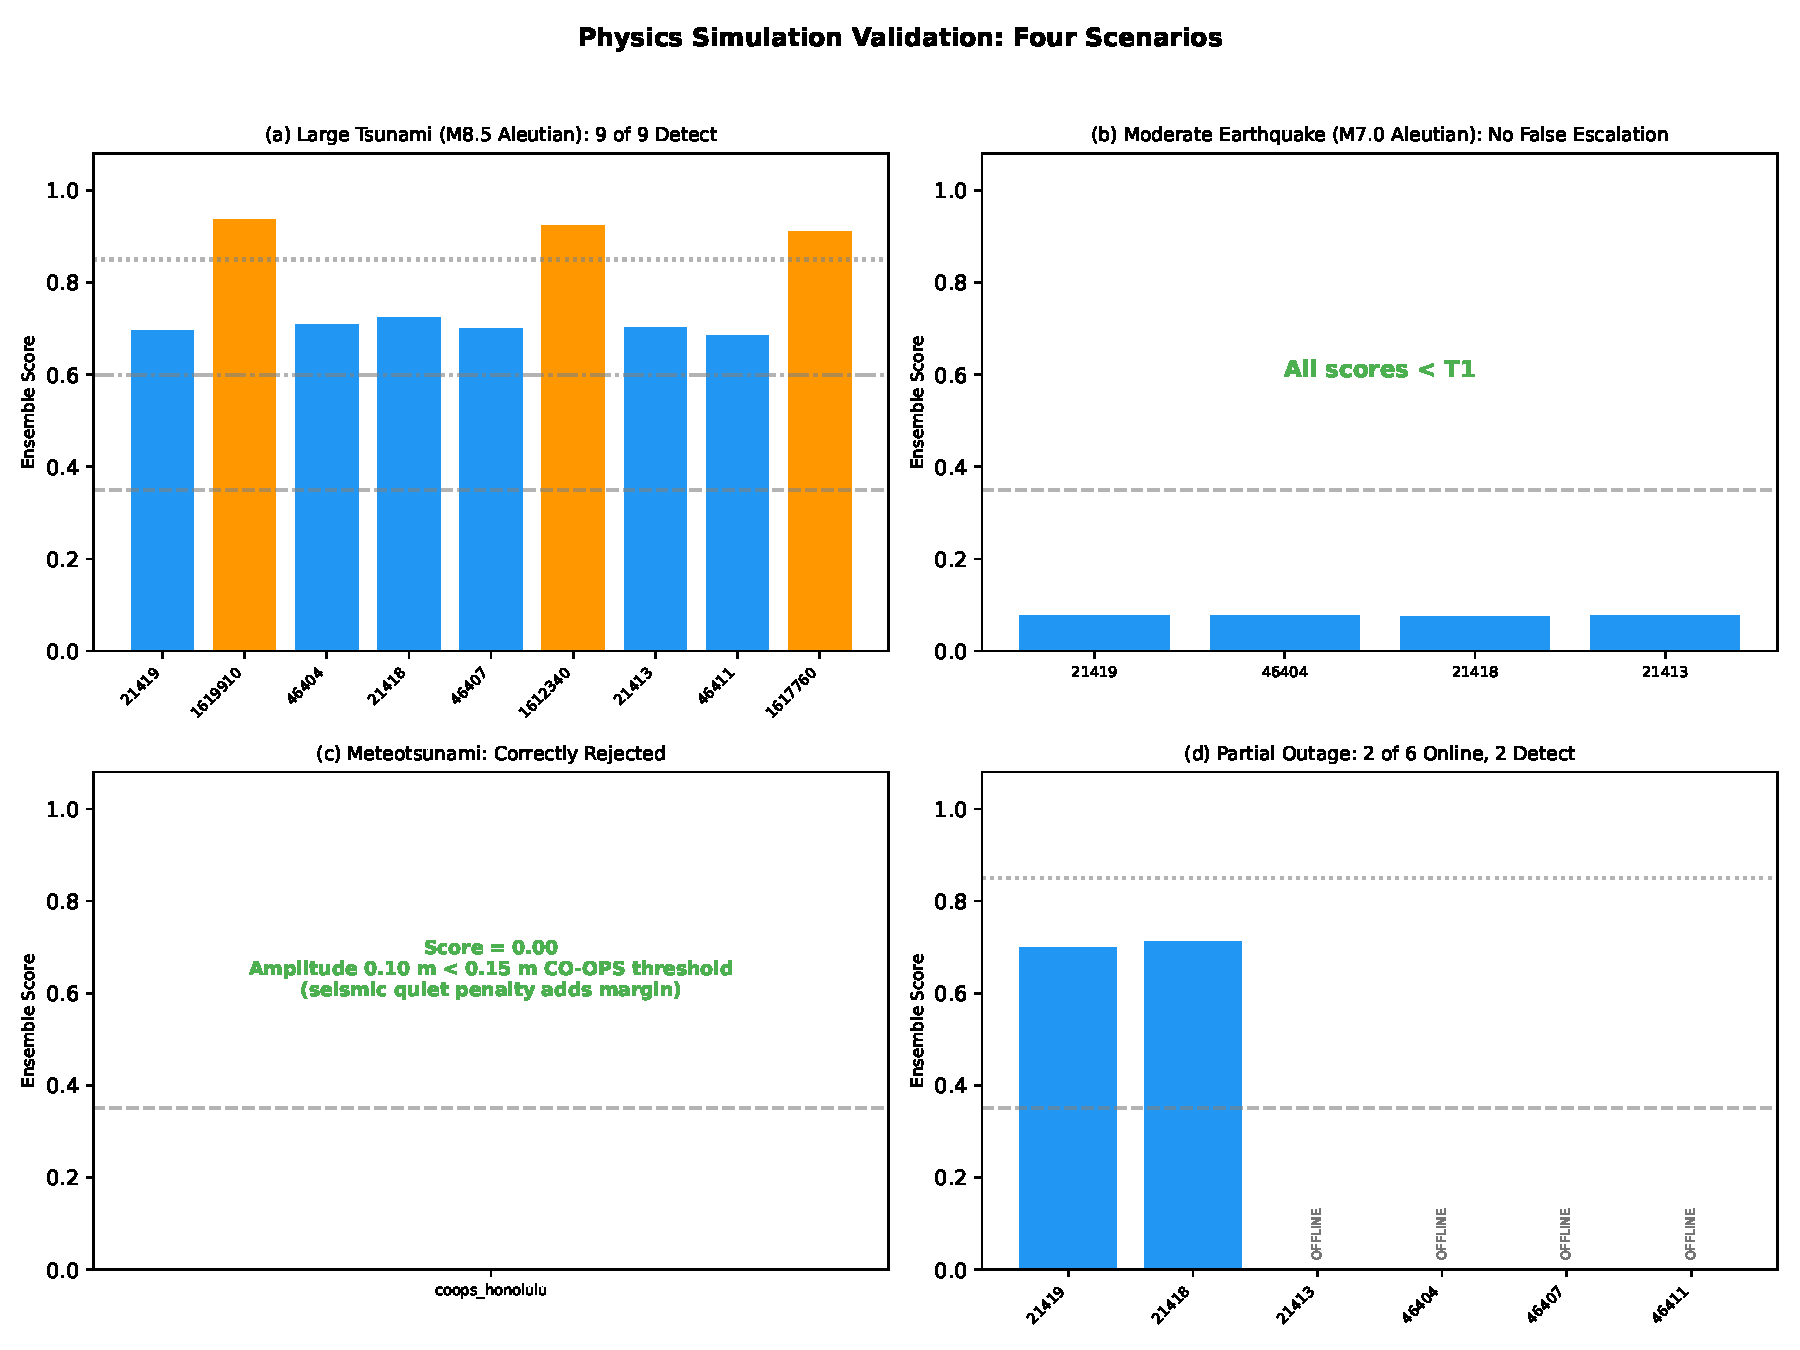
\includegraphics[width=\linewidth]{figures/fig_physics_summary.pdf}
\caption{Four-scenario physics simulation summary.
  (a)~M8.5 Aleutian large tsunami: stations within detection range.
  (b)~M7.0 moderate earthquake: zero false escalation.
  (c)~Meteotsunami: correctly rejected; the 0.10\,m amplitude is below
  the 0.15\,m CO-OPS detection threshold (the seismic quiet penalty
  adds margin but is not the primary rejection mechanism).
  (d)~Partial outage: 2 of 6 online stations detect, both exceeding
  $T_2$.}
\label{fig:physics-summary}
\end{figure}

\begin{figure}[htbp]
\centering
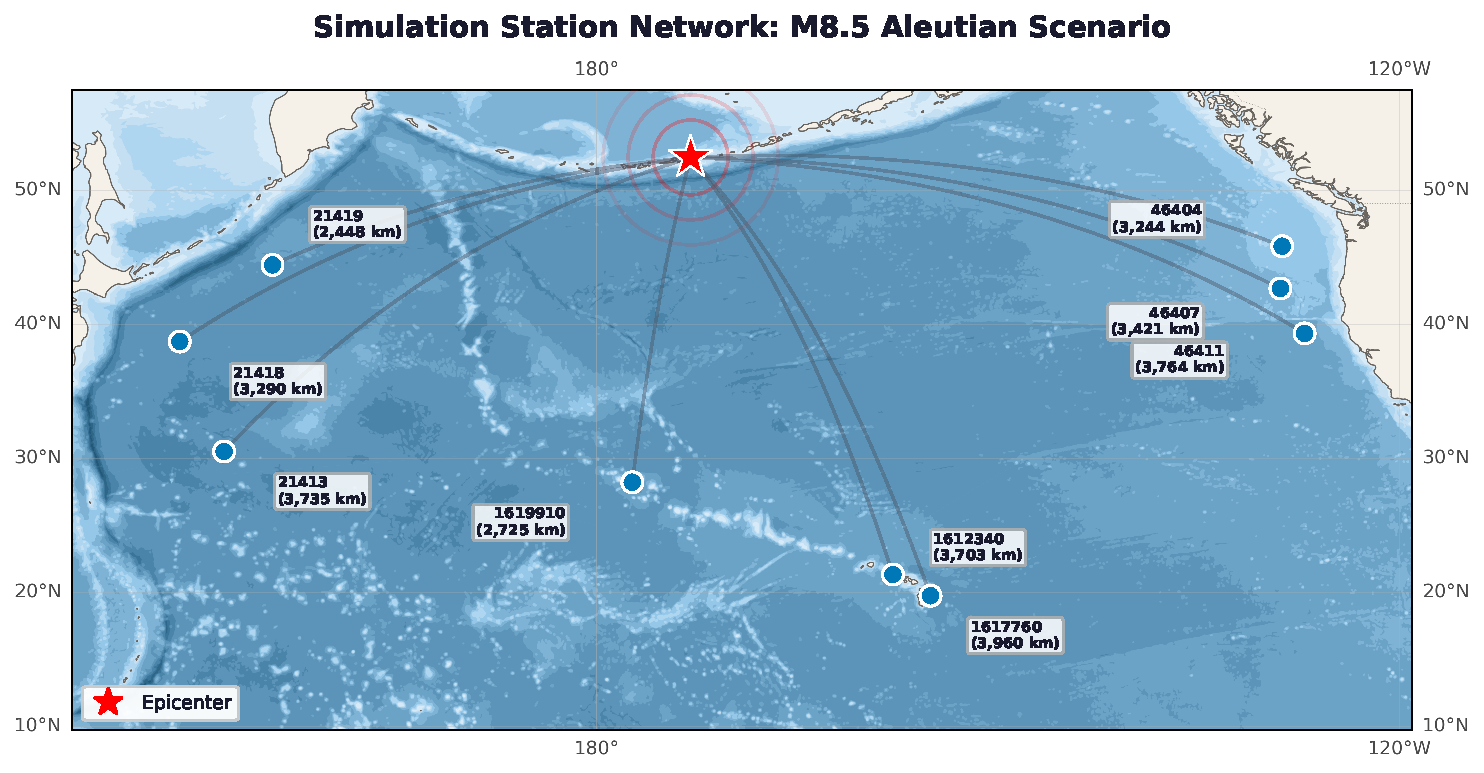
\includegraphics[width=0.92\linewidth]{figures/fig_simulation_station_map.pdf}
\caption{Simulation station network for Scenario~1 (M8.5 Aleutian).
  Red star marks the synthetic epicenter; circles show the six Pacific
  DART stations and three CO-OPS tide gauge stations used in the
  simulation framework.}
\label{fig:simulation-station-map}
\end{figure}

\paragraph{Synthetic waveform evolution.}
Figure~\ref{fig:simulation-station-map} shows the simulation station
network for Scenario~1.
Figure~\ref{fig:synthetic-waveforms} shows the raw synthetic records
at all nine stations (six DART bottom-pressure recorders and three
CO-OPS tide gauges).  DART station amplitudes (0.025--0.032\,m) reflect
the combined effects of geometric spreading (distances
2{,}448--3{,}764\,km) and azimuthal directivity: the Aleutian
fault strike (250\textdegree) directs maximum radiation NNW, whereas
the Pacific stations lie south or east of the epicenter, receiving
40--50\% of the peak amplitude.  CO-OPS coastal stations show
${\sim}10\times$ larger amplitudes (0.23--0.28\,m) due to Green's Law
shoaling amplification (${\sim}3.8$--$4.5\times$) applied at nearshore depths
of 10--20\,m, plus larger tidal and noise baselines.
Figure~\ref{fig:synthetic-residuals} presents the corresponding
detided residuals, isolating the tsunami signal from the tidal
background; shared Y-axes and an overlay comparison panel make the
amplitude variation and arrival-time progression visible across stations.

\begin{figure}[htbp]
\centering
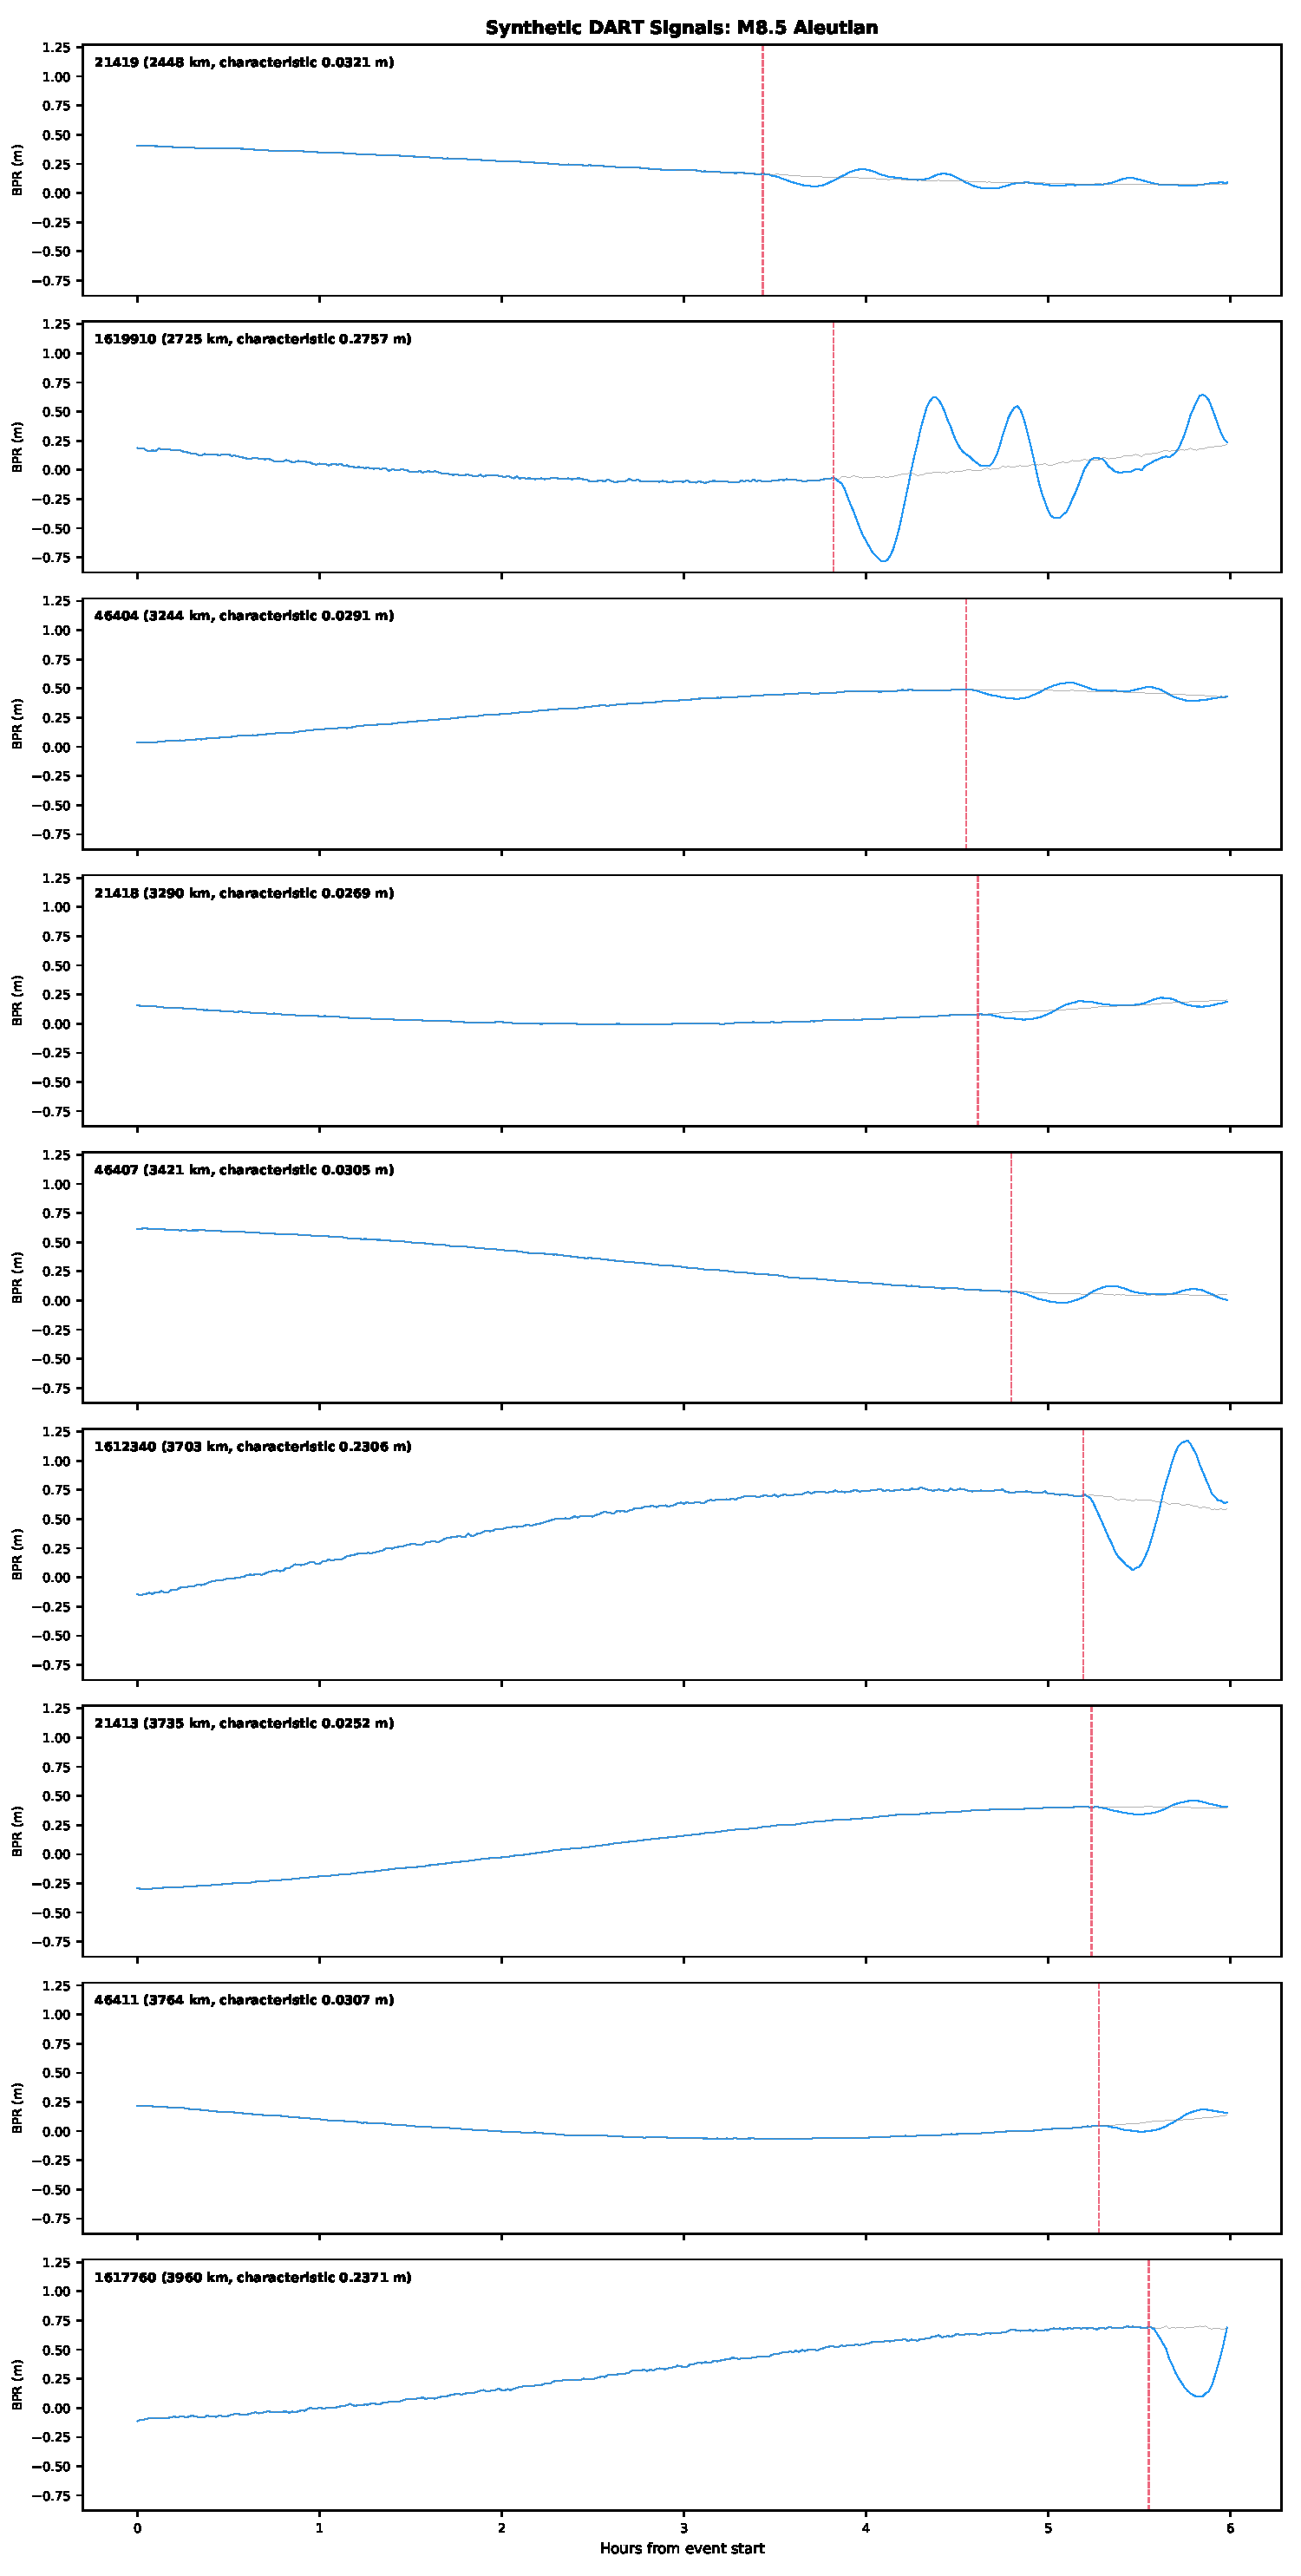
\includegraphics[width=\linewidth,height=0.88\textheight,keepaspectratio]{figures/fig_synthetic_waveforms.pdf}
\caption{Raw synthetic records for the M8.5 Aleutian scenario
  (Scenario~1) at six Pacific DART stations and three CO-OPS tide
  gauges.  DART stations carry ${\sim}$0.03\,m characteristic tsunami
  amplitudes on a tidal baseline with instrument drift; CO-OPS stations
  carry ${\sim}$0.25\,m after Green's Law shoaling amplification.  The
  value in each panel label is that characteristic amplitude, not the peak
  of the plotted record, which also contains the tide, drift and noise.
  Vertical dashed lines mark predicted tsunami arrival times.}
\label{fig:synthetic-waveforms}
\end{figure}

\begin{figure}[htbp]
\centering
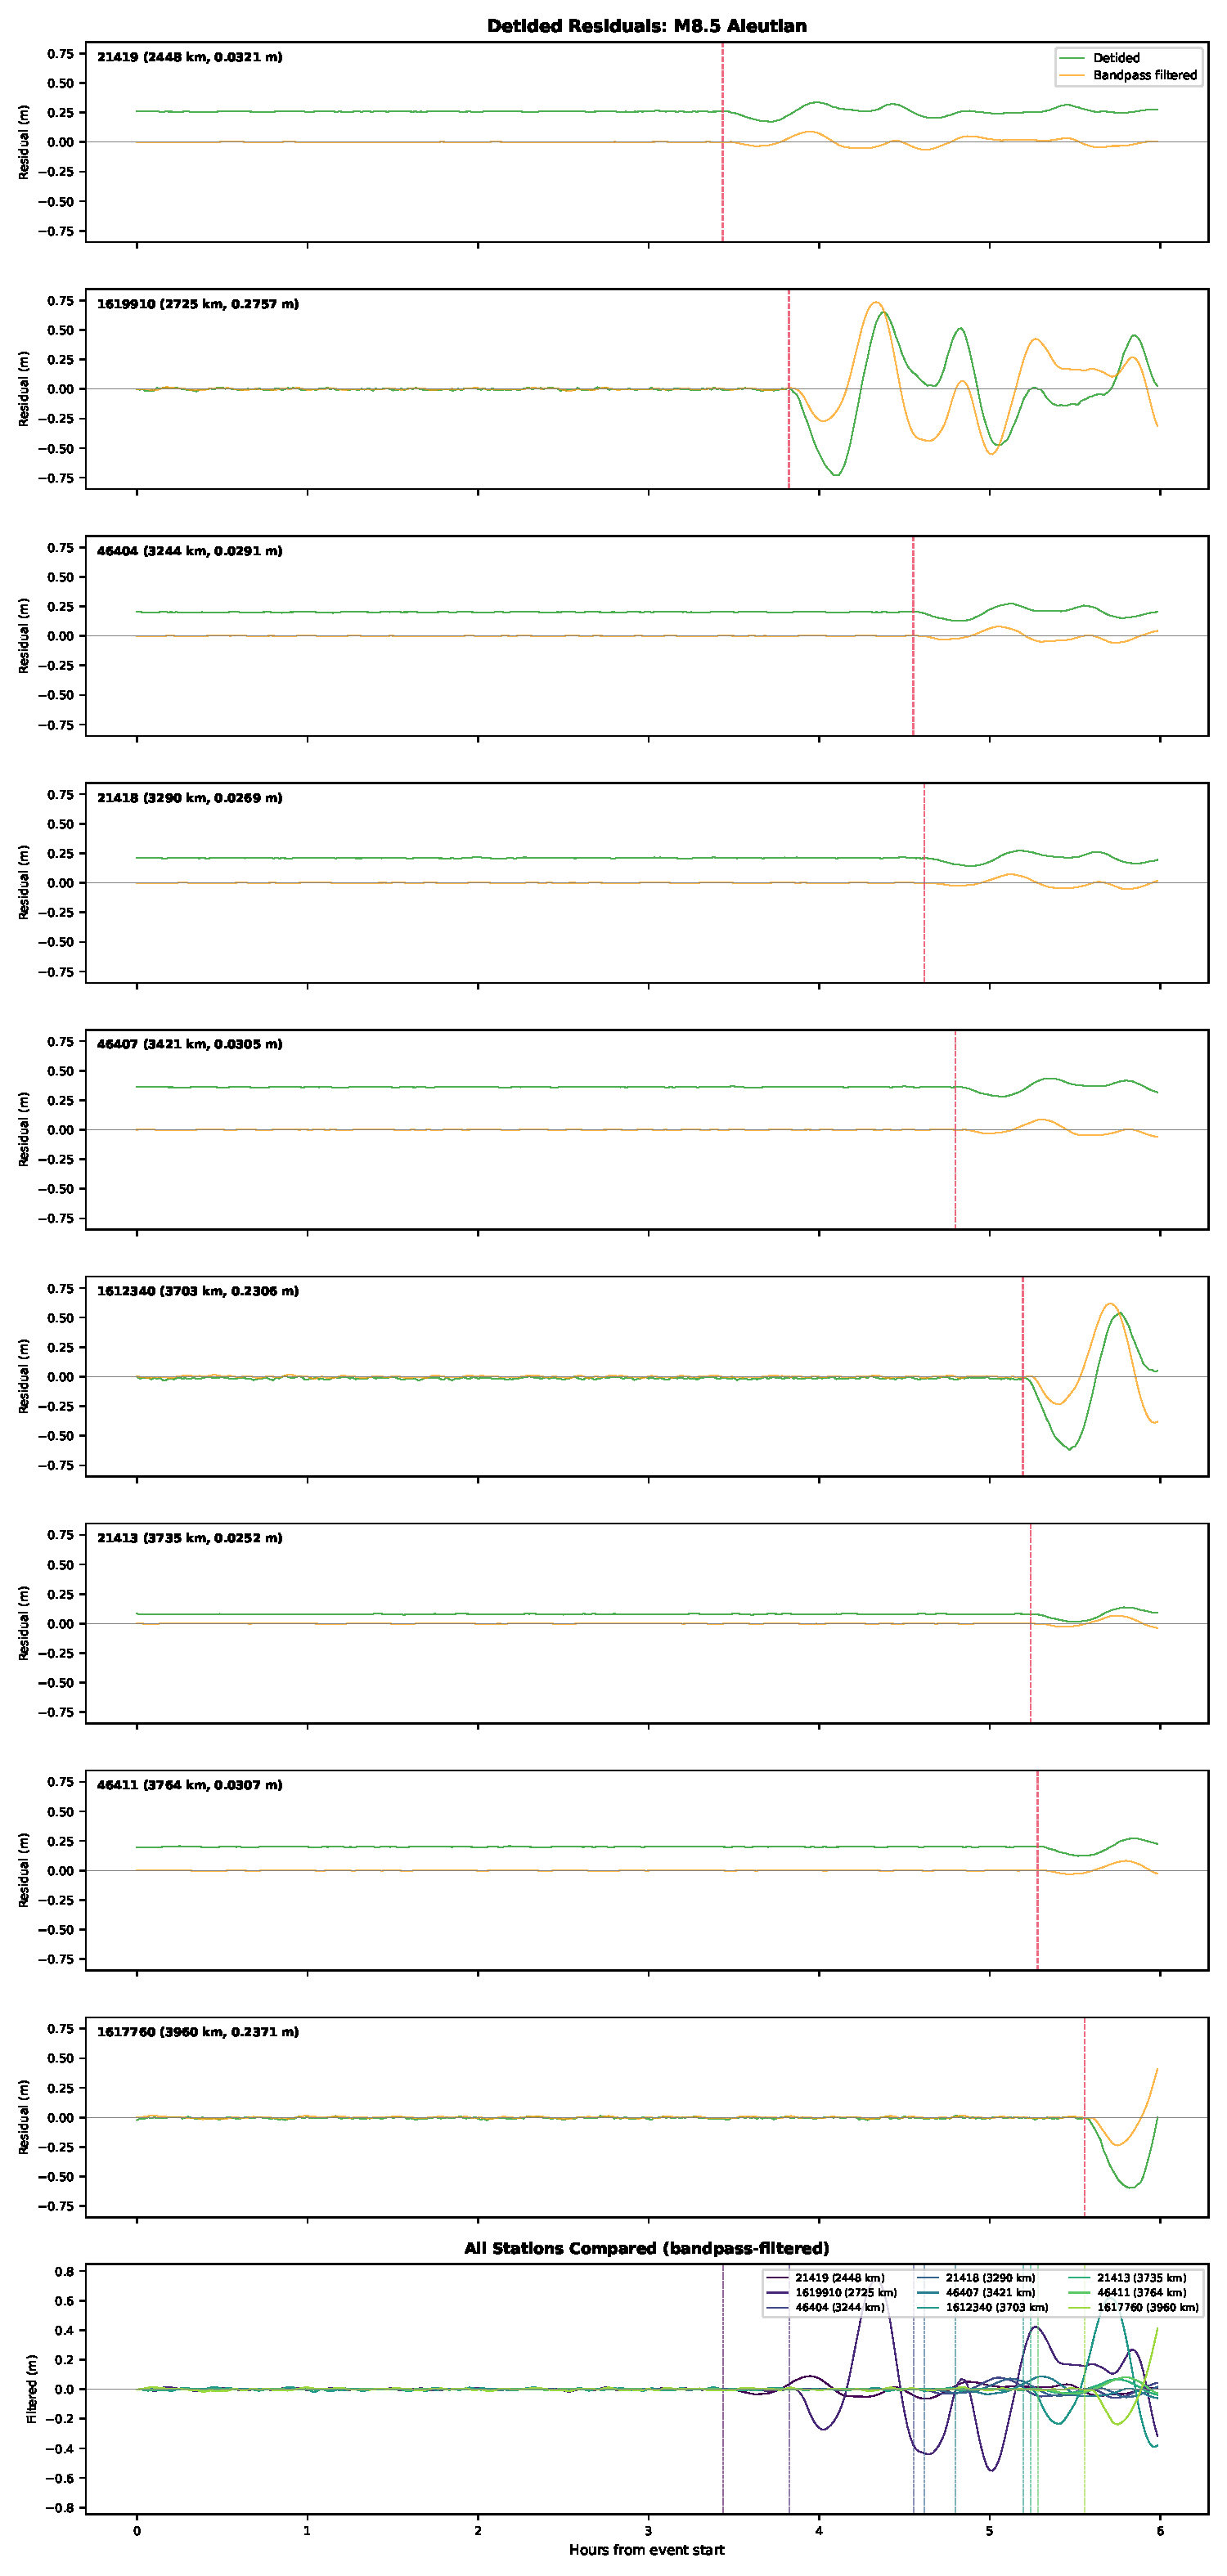
\includegraphics[width=\linewidth,height=0.88\textheight,keepaspectratio]{figures/fig_synthetic_residuals.pdf}
\caption{Detided residuals for Scenario~1 showing the isolated
  tsunami signal after harmonic removal and bandpass filtering
  (5--120\,min passband).  Green: full-frequency residual; orange:
  bandpass-filtered signal used by the threshold detector.  Shared
  Y-axes make the amplitude variation across stations visible
  (station type dominates: the CO-OPS gauges are Green's-Law
  amplified, and azimuthal directivity modulates the DART
  amplitudes); the bottom overlay panel compares all stations on
  one axis.  Each panel label reports the characteristic amplitude
  carried to that station, which is the input to the simulation rather
  than a measurement of the trace beside it; the plotted residual peaks
  roughly two to three times higher, because the synthesized waveform
  sums many spectral components.}
\label{fig:synthetic-residuals}
\end{figure}

\paragraph{Detection score evolution.}
Figure~\ref{fig:synthetic-score-timeline} compares the
sliding-window score evolution for the M8.5 Aleutian (left column,
all nine stations: six DART and three CO-OPS) and M7.0 moderate
(right column, three stations)
scenarios.  For the M8.5 event, the detector scores rise after tsunami
arrival at each station, with the ensemble score crossing $T_1$
(\textsc{investigate}) at all six DART stations and $T_2$
(\textsc{assess}) at five of six.  The reduced amplitudes
(0.025--0.032\,m) from directivity and realistic tidal backgrounds
prevent $T_3$ (\textsc{escalate}) crossings at the six DART stations
within the sliding-window timelines; two of the three CO-OPS stations
cross $T_3$ in the timelines, and all three do so on the full event
window due to Green's-Law shoaling amplification (see above).  The onset time varies by station, reflecting the
206--333\,min spread in arrival times across the nine stations.  For the
M7.0 event, the scores remain near zero throughout, confirming correct
rejection of the non-tsunamigenic signal.

\begin{figure}[htbp]
\centering
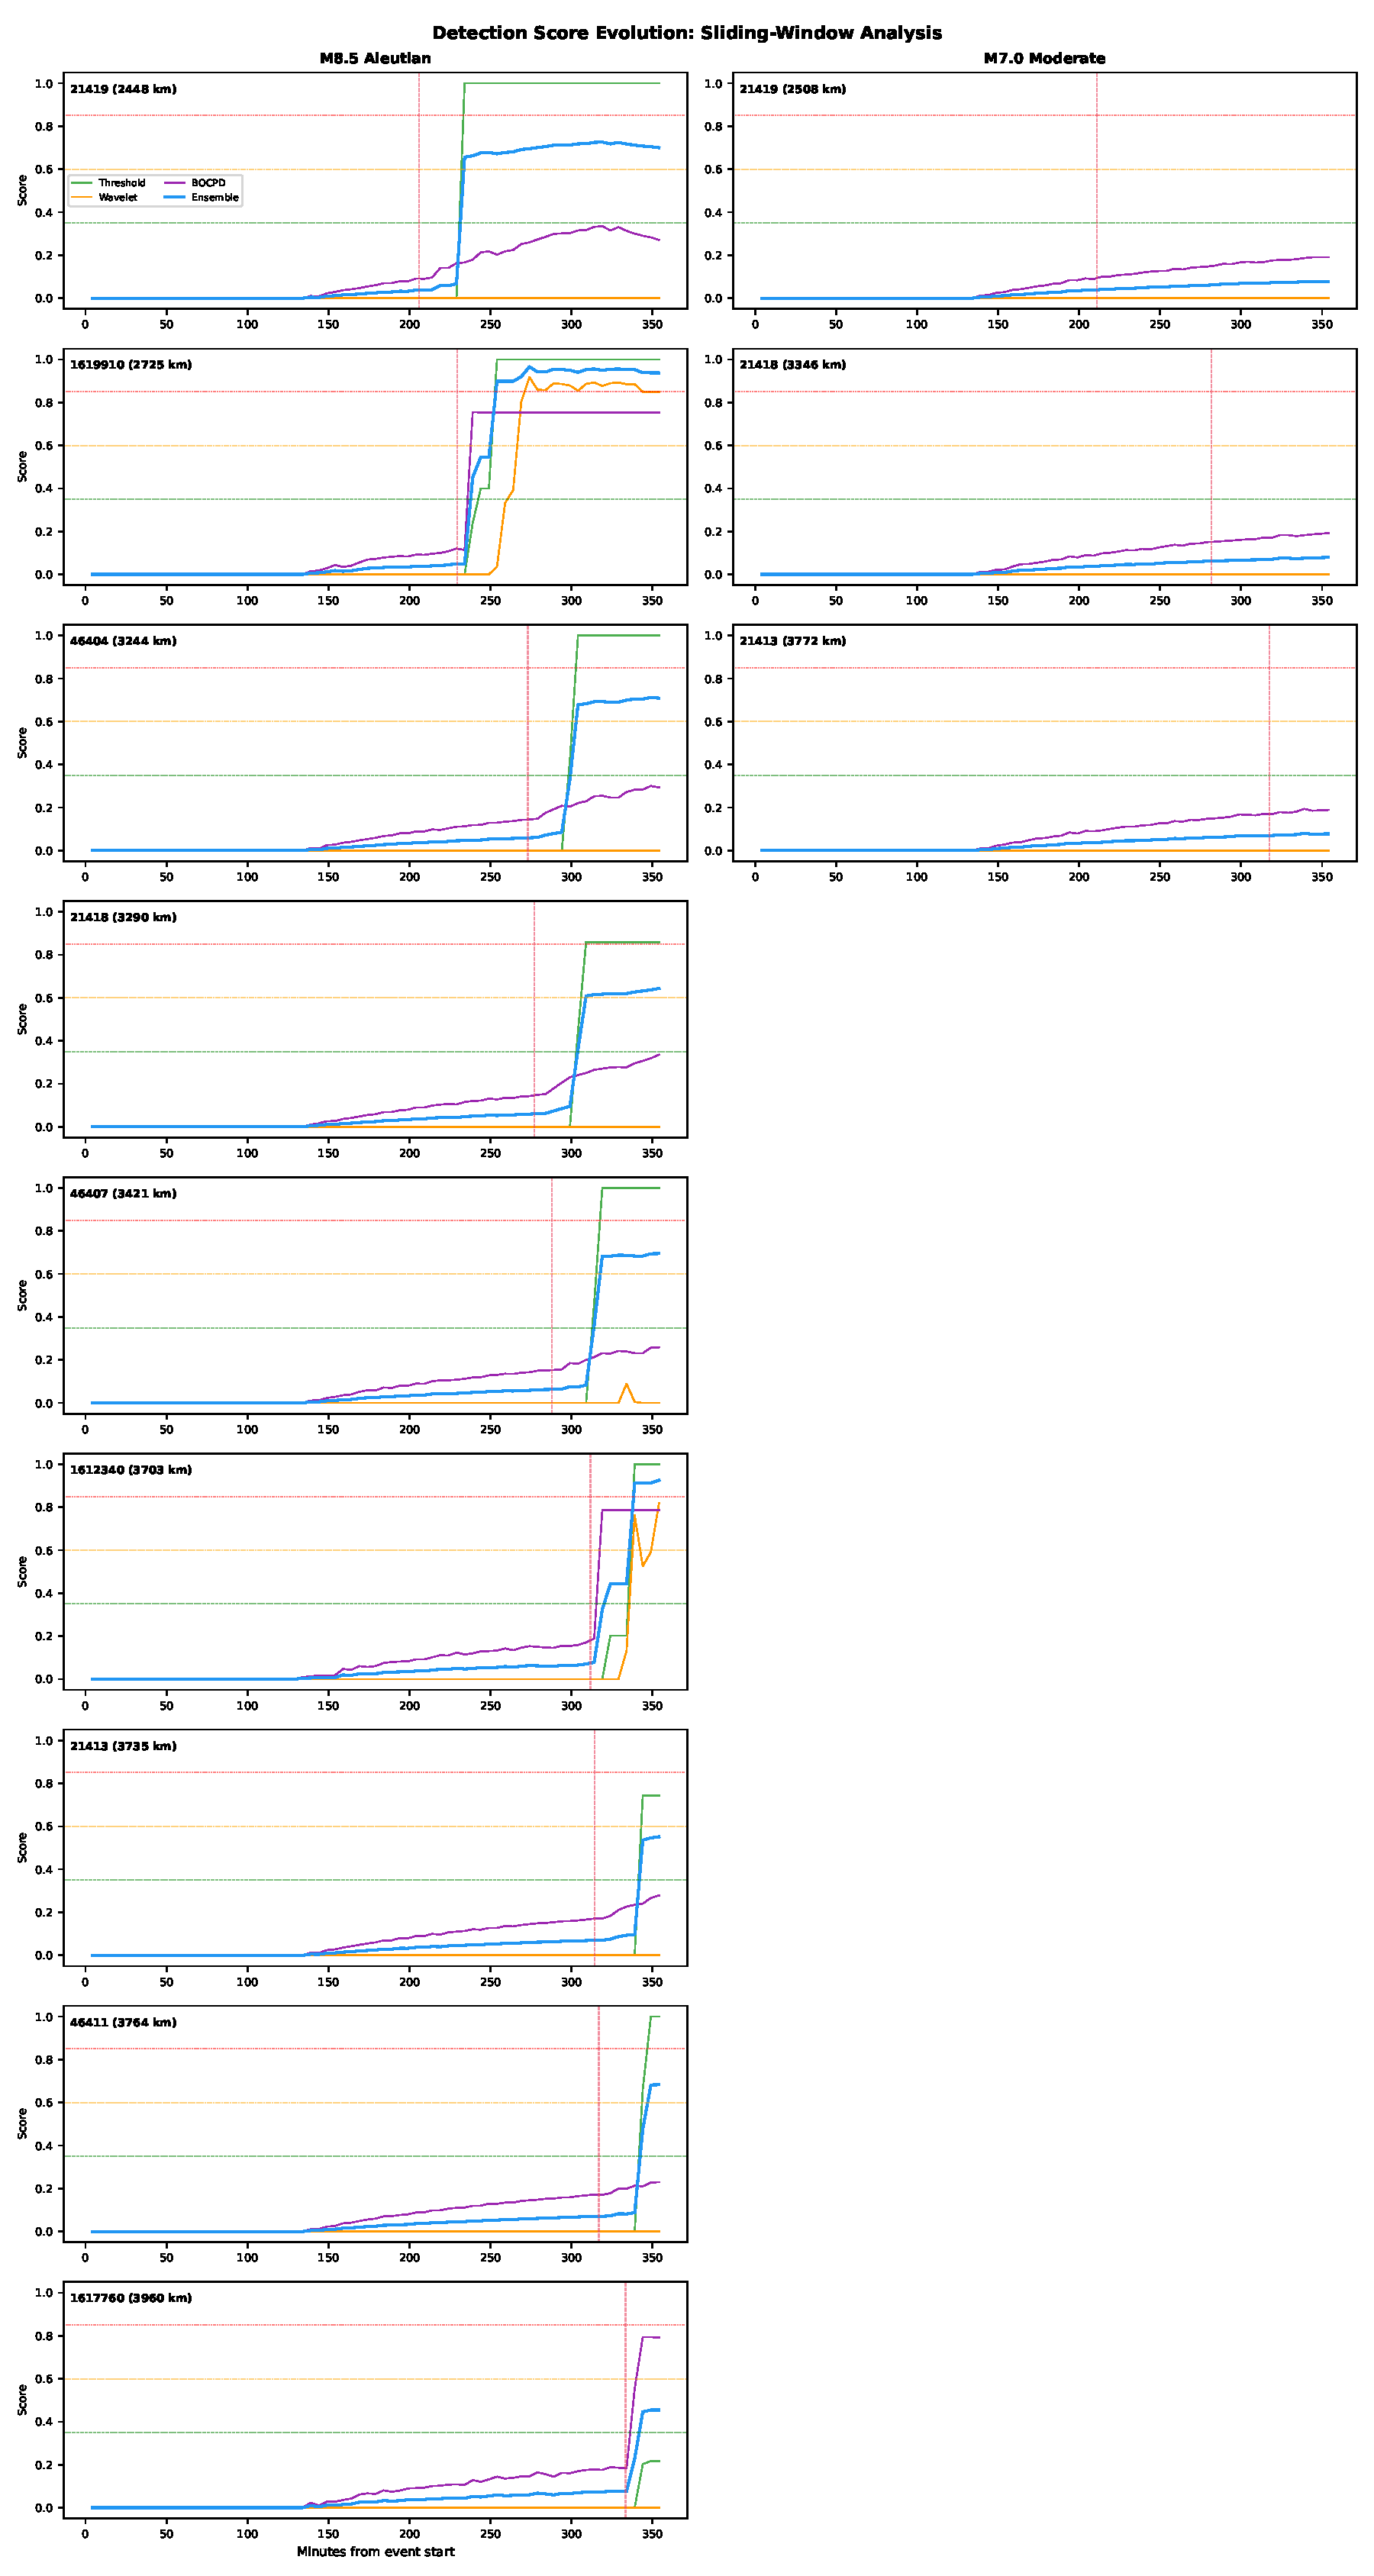
\includegraphics[width=\linewidth,height=0.88\textheight,keepaspectratio]{figures/fig_synthetic_score_timeline.pdf}
\caption{Sliding-window detection score evolution.
  Left column: M8.5 Aleutian scenario (all nine stations: six DART,
  three CO-OPS) showing
  rapid threshold crossings after tsunami arrival at each station.
  Right column: M7.0 moderate earthquake (three stations) showing
  correct rejection (all scores remain below $T_1 = 0.35$).
  Colors: blue = ensemble, green = threshold, orange = wavelet,
  purple = BOCPD.  Horizontal lines mark $T_1$, $T_2$, $T_3$.}
\label{fig:synthetic-score-timeline}
\end{figure}

\paragraph{Waveform realism.}
The simulation generates multi-frequency tsunami spectra with 10
components following an $\omega^{-2}$ rolloff above the corner frequency,
N-wave polarity for thrust-fault events ($\pi$-phase on flat-spectrum
components), and weak Boussinesq dispersion via the exact dispersion
relation~\citep{kajiura1963leading}.
Frequency-dependent coda decay
(Rabinovich et~al.~\citep{rabinovich2013nearfield}) uses a 600-min
base timescale scaled by period: $\tau(T) = 600 \cdot (1 + T/30)$\,min,
so short-period components (5\,min) decay in ${\sim}700$\,min while
long-period components (60\,min) persist for ${\sim}1{,}800$\,min,
consistent with observed trans-Pacific energy decay times of 15--29\,h.
DART bottom-pressure records include station-specific instrumental
drift (0.1--0.5\,mm/h, Watts \& Kontoyiannis~\citep{watts1990drift}).
CO-OPS tide gauge signals receive Green's Law shoaling amplification
and higher tidal/noise baselines.

Several further physics improvements are identified for future work:
dual dominant periods from fault length and width
(Heidarzadeh \& Satake~\citep{heidarzadeh2013waveform}),
canonical $\operatorname{sech}^2 \cdot \tanh$ N-wave shape
(Tadepalli \& Synolakis~\citep{tadepalli1994model}),
longer coda with basin reverberations
(Mofjeld et~al.~\citep{mofjeld2001scattering}),
configurable Comer slope, and kinematic rupture directivity
(Sementsov et~al.~\citep{sementsov2025kinematic}).
These enhancements would improve waveform morphology fidelity but
are parametric approximations, not substitutes for physics-based
models (e.g., MOST, GeoClaw).

% ============================================================
%  7. Discussion
% ============================================================

\section{Discussion}
\label{sec:discussion}

\paragraph{Comparison with direct LLM pipelines.}
A fully LLM-driven pipeline (e.g., using an agentic framework where
the language model controls routing decisions) would offer greater
flexibility but at the cost of determinism and auditability. Tsunami
assessment is a domain where the ability to exactly reproduce a
reasoning trace hours after an event is operationally essential. The
deterministic FSM and rule-based routing produce identical state
transitions for identical inputs, regardless of model version or
inference temperature.

\paragraph{Comparison with DART detection methods.}
Table~\ref{tab:method-comparison} compares the proposed system with
existing DART-based tsunami detection algorithms on key design axes.
Our system trades minimal data requirements (30-day calibration vs.\
3~hours for Mofjeld) for physically interpretable detiding,
multi-component ensemble scoring, and integrated verification with
safety controls. The computational overhead of the ensemble
(${\sim}47$\,ms p95) is negligible relative to the data polling
interval (15--60\,s). No prior DART detection method integrates
verification checks, human-in-the-loop gating, or structured
abstention.

\begin{table}[!htb]
\centering
\caption{Comparison of DART-based tsunami detection methods.
  $^\dagger$Compute latency per station per observation window.
  $^\ddagger$Not directly benchmarked on the same data; values from
  respective publications.}
\label{tab:method-comparison}
\footnotesize
\setlength{\tabcolsep}{3pt}
\begin{tabular}{p{2.4cm}p{2.4cm}p{2.2cm}p{1.4cm}p{1.1cm}p{2.3cm}}
\toprule
\textbf{Method} & \textbf{Tidal Removal} & \textbf{Detection} & \textbf{Data Req.} & \textbf{Lat.$^\dagger$} & \textbf{Verification} \\
\midrule
Mofjeld TDA~\citep{mofjeld1997tsunami}
  & Cubic polynomial & Amplitude threshold & 3\,h prior & $\sim$ms & None \\[3pt]
Chierici~\citep{chierici2017new}
  & Harmonic + filter & Modular (bandpass) & $\sim$2\,mo & $\sim$min$^\ddagger$ & None \\[3pt]
Beltrami~\citep{beltrami2008ann}
  & (ANN internal) & Neural network & Training set & $\sim$ms$^\ddagger$ & None \\[3pt]
Wang~\citep{wang2020realtime}
  & EEMD & Mode decomposition & $\sim$3\,h & $\sim$min$^\ddagger$ & None \\[3pt]
\textbf{This work}
  & 8-const.\ harmonic (IRLS, 30\,d) & Ensemble (3{+}1 components) & 30\,d cal. & 47\,ms & 9 checks + ABSTAIN \\
\bottomrule
\end{tabular}
\end{table}

\paragraph{ABSTAIN as a safety property.}
The ABSTAIN output is an explicit design choice, not a fallback.
A system that suppresses uncertain outputs rather than communicating
its uncertainty can create a false impression of reliability. By
treating ABSTAIN as an explicit, structured output routed through
the same Human Review Gate as positive assessments, the framework
tells a duty scientist why it withheld guidance instead of returning
nothing.

\paragraph{LLM synthesis layer.}
The implemented 4-node synthesis graph shows that
LLM-generated operator narratives can be attached to a deterministic
pipeline without changing what that pipeline decides. Three
design choices maintain determinism under LLM integration: (1)~system confidence
is computed deterministically \emph{before} any LLM call, so the
LLM never self-reports confidence; (2)~the template-rendered
output is always computed first and is always the emitted report
text, with the LLM narrative stored separately as advisory
commentary that is dropped outright if the LLM call fails or its
output fails the guardrail scan; and (3)~structured output
schemas (Pydantic models via
\texttt{with\_structured\_output}) constrain the LLM to produce
only the fields the downstream pipeline expects. This constrains
the output structure; it does not verify the factual accuracy of
numbers the model may quote within narrative fields.
The test suite confirms that the guardrail cascade (LLM output
scanned, commentary dropped, template stands) activates
correctly when the
LLM produces prohibited NOAA alert terminology, though systematic
evaluation across diverse event scenarios remains future work.

\paragraph{Latency budget.}
Table~\ref{tab:latency} summarizes the per-component latency targets and
estimated budgets. Ingest and QC latencies are bounded by external
API polling intervals and lightweight QARTOD checks. The anomaly
detection pipeline (detide, bandpass filter, wavelet, BOCPD, and
optional Isolation Forest) completes in ${\sim}47$\,ms (p95) for
single-station data on a single core (Table~\ref{tab:latency},
AnomalyAgent end-to-end row). Scenario inversion dominates the end-to-end
budget because the NNLS solver (Eq.~\ref{eq:nnls}) iterates over the propagation database;
the 3-minute target assumes a pre-loaded database with ${\leq}200$
candidate subfaults. When the LLM synthesis layer is enabled, a single
API call (evidence, scenario, or narrative node) adds 3--8\,s of wall-clock
time, but runs on the template-only path in $<1$\,s when the API is
unavailable. The end-to-end target of ${\leq}5$ minutes from data
availability to Tier~1 report is within the same order of magnitude as
the PTWC's initial bulletin timeline~\citep{bernard2015evolution},
though the two are not directly comparable: the PTWC clock starts at
earthquake origin, whereas ours starts when DART data become available.

\begin{table}[ht]
\centering
\caption{Latency budget by pipeline component.
  Measured values from \texttt{scripts/profile\_latency.py}
  (50 iterations, Apple M-series laptop);
  network-dependent components show design targets.}
\label{tab:latency}
\small
\begin{tabular}{lrrl}
\toprule
\textbf{Component} & \textbf{p50 (ms)} & \textbf{p95 (ms)} & \textbf{Notes} \\
\midrule
DART ingest (event mode) & --- & $\leq 30{,}000$ & 15\,s poll + HTTP (design target) \\
Seismic ingest & --- & $\leq 15{,}000$ & FDSN event query (design target) \\
QC (10 records) & 0.12 & 0.16 & 5 QARTOD checks (measured) \\
Detide + bandpass & 0.90 & 1.10 & Harmonic fit + Butterworth (measured) \\
Anomaly detection (full) & 43.5 & 44.4 & BOCPD dominates (measured) \\
AnomalyAgent end-to-end & 44.8 & 46.8 & Detide + all scores (measured) \\
FSM transition & 0.01 & 0.02 & In-memory lookup (measured) \\
Scenario inversion & --- & $\leq 180{,}000$ & NNLS + bootstrap UQ (design target) \\
Report (template) & --- & $\leq 1{,}000$ & Python f-string (design target) \\
Report (LLM-enhanced) & --- & $\leq 30{,}000$ & 3 LLM API calls (design target) \\
Human Review Gate & \multicolumn{2}{c}{Variable} & Operator decision \\
\bottomrule
\end{tabular}
\end{table}

\paragraph{Retrospective validation.}
The retrospective evaluations (Section~\ref{sec:evaluation}) reveal
both the strengths and boundaries of the current design.
The ensemble detector reliably escalates near-field stations
across all five events; however, the earliest detections at the
closest stations (e.g., 3.6~min at 560~km for Tohoku, 12.3~min at
2{,}400~km for Chile) reflect coseismic pressure perturbations rather
than tsunami waves, making them useful as triggers for further
investigation rather than as direct tsunami confirmations.
The quiet-period evaluation (15~days at 15-minute standard-mode
sampling; Section~\ref{sec:eval-false-positive}) produced one false trigger
across 414 windows (${\sim}0.29$ per station-month), but the full
ensemble in event-mode sampling remains untested against background
ocean noise.
We report detection at fixed FSM operating points rather than
swept-threshold metrics (ROC, AUC) because the FSM thresholds are
design constants, not learned decision boundaries; future work
should calibrate these thresholds against a larger event catalog.

\paragraph{Cross-event detection consistency.}
Across all five retrospective case studies, event-mode stations
within $\sim$3{,}000\,km of the epicenter consistently reach at
least the INVESTIGATE threshold ($T_1 = 0.35$), and the nearest
station reaches ASSESS or ESCALATE in four of the five events.
The exception is Samoa 2009, where the nearest station (51425 at
804\,km) reaches only INVESTIGATE at 0.588 while 51426 at 935\,km
reaches ESCALATE, so proximity alone does not order the scores.
Detection scores generally decrease with distance for a
given event, consistent with geometric spreading, though
far-field stations may show elevated scores from seismic
contamination (as observed for T\={o}hoku stations 46408 and
46402, where coseismic pressure perturbations dominate).
The three additional case studies (Illapel 2015, Iquique 2014,
Samoa 2009; Appendix~\ref{sec:appendix-case-studies}) extend the
descriptive cross-event check: the same ensemble weights and FSM
thresholds produce similar operating-point behavior across five
distinct historical events spanning $M_w$\,8.1--9.1, two tectonic
mechanisms (thrust and outer-rise normal faulting), and epicentral
distances from 295 to 15{,}840\,km. Because all five events were
available during development and review, this consistency is not a
held-out test and cannot exclude parameter tuning.

Figure~\ref{fig:latency-distance} shows threshold-crossing latency as a
function of epicentral distance across all five events. Most plotted
crossings precede the simple $d/198$\,m/s tsunami-travel reference, but
not all do: Iquique station 32413 crosses INVESTIGATE at 266.2~min,
compared with a 236.4~min reference at 2{,}809~km. Event-mode status is
a transmission state rather than a measured tsunami arrival, and the
retrospective comparison does not establish operational warning lead
time. Replay timing excludes live ingest, transmission, and processing
delays.
All detections fall at or after the P-wave arrival curve
(${\sim}8$\,km/s); the far-field crossings track Rayleigh-wave
group velocities (${\sim}3.5$--$3.8$\,km/s), consistent with
seismic rather than tsunami energy.
Figure~\ref{fig:component-strip} reveals component-level score
distributions across events: the threshold detector frequently
saturates at 0 or 1.0, while the wavelet and BOCPD components
provide intermediate discrimination that drives the ensemble
into the INVESTIGATE and ASSESS ranges.
Figure~\ref{fig:noise-triptych} demonstrates detection robustness
across a $10\times$ range of ambient noise levels
(0.5--5\,mm standard deviation), showing that the ESCALATE boundary
shifts upward by roughly a factor of three (about half an amplitude
decade) at most periods under the noisiest conditions, and moves
beyond the tested amplitude range at the longest periods
(90--120\,min).

\begin{figure}[!htbp]
\centering
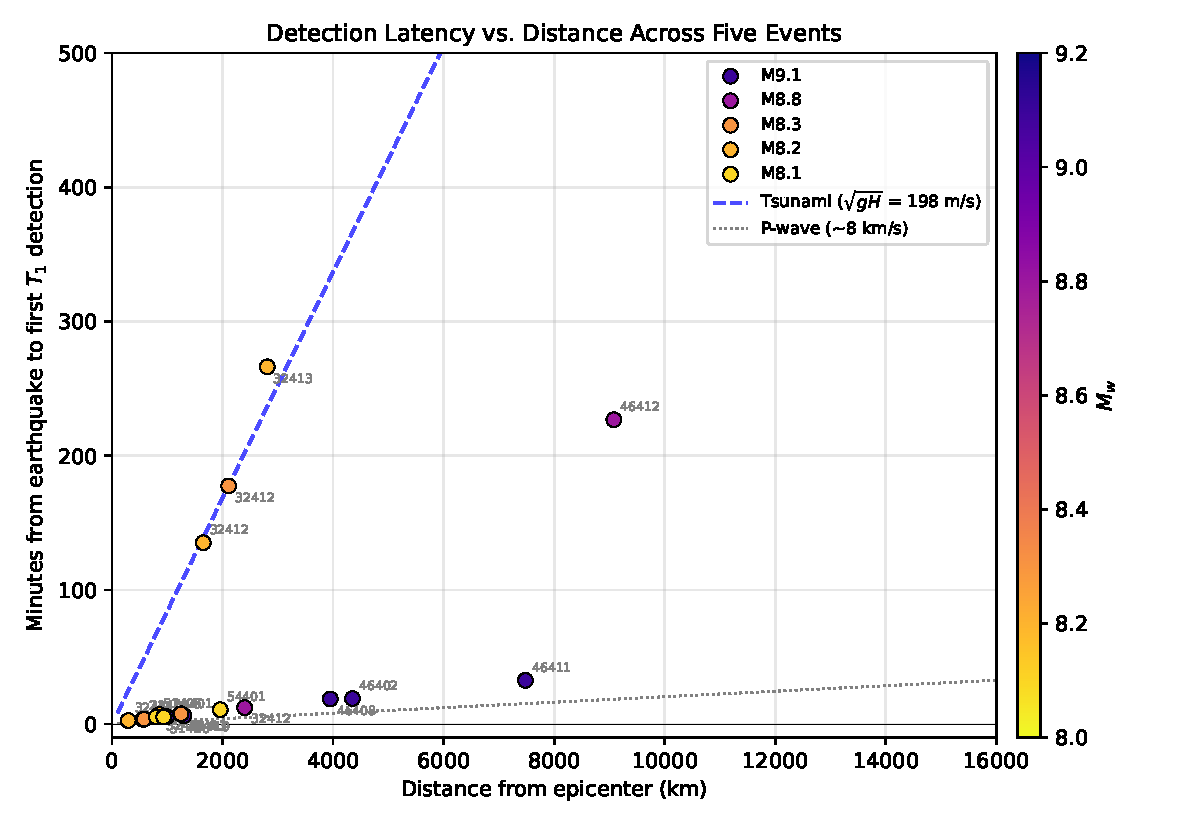
\includegraphics[width=\linewidth]{figures/fig_latency_vs_distance.pdf}
\caption{Detection latency vs.\ epicentral distance across all five
  retrospective events.  Each point represents a DART station's first
  $T_1$ threshold crossing in the sliding-window analysis.  Blue dashed
  line: theoretical tsunami travel time at deep-ocean speed
  ($\sqrt{gH} = 198$\,m/s).  Gray dotted: P-wave arrival
  (${\sim}8$\,km/s).  Color encodes earthquake
  magnitude $M_w$.}
\label{fig:latency-distance}
\end{figure}

\begin{figure}[!htbp]
\centering
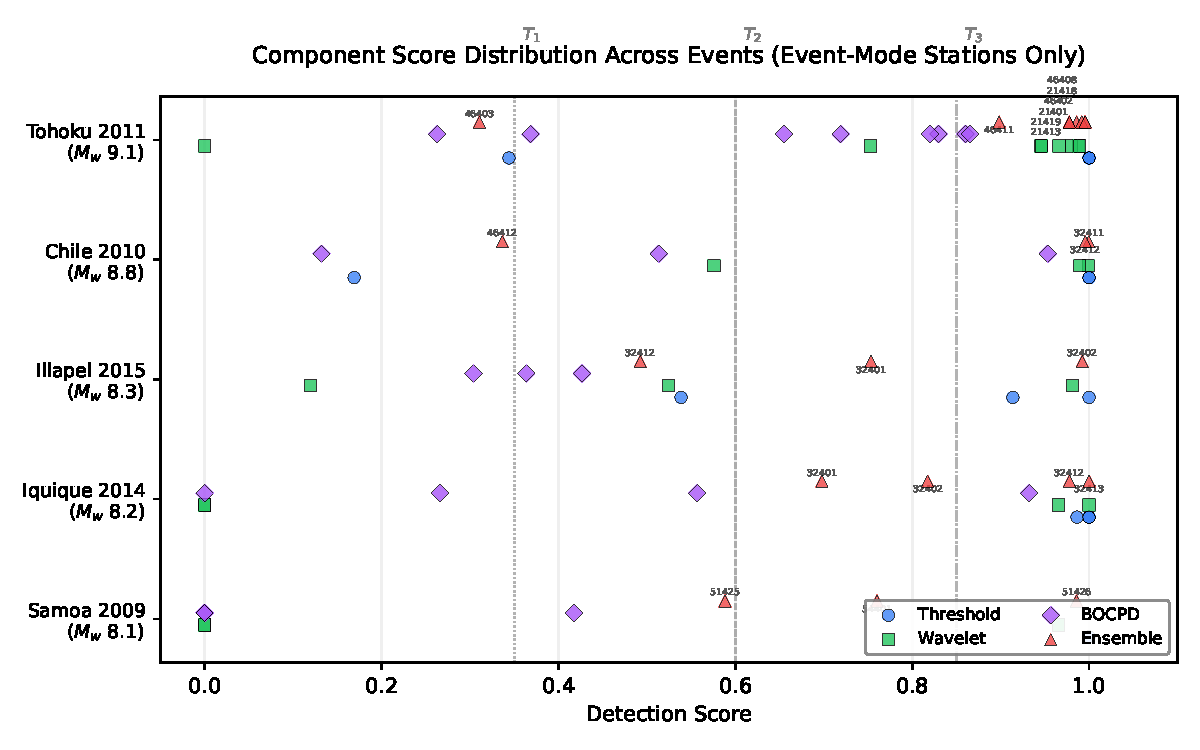
\includegraphics[width=\linewidth]{figures/fig_component_score_strip.pdf}
\caption{Component score distributions for event-mode DART stations
  across five events.  Each station contributes four markers (threshold,
  wavelet, BOCPD, ensemble).  Vertical gray lines mark FSM thresholds
  $T_1$, $T_2$, $T_3$.  The threshold detector often saturates
  near 0 or 1.0 but produces intermediate values at marginal
  stations; wavelet and BOCPD provide graded scores that drive
  ensemble positioning between thresholds.}
\label{fig:component-strip}
\end{figure}

\begin{figure}[!htbp]
\centering
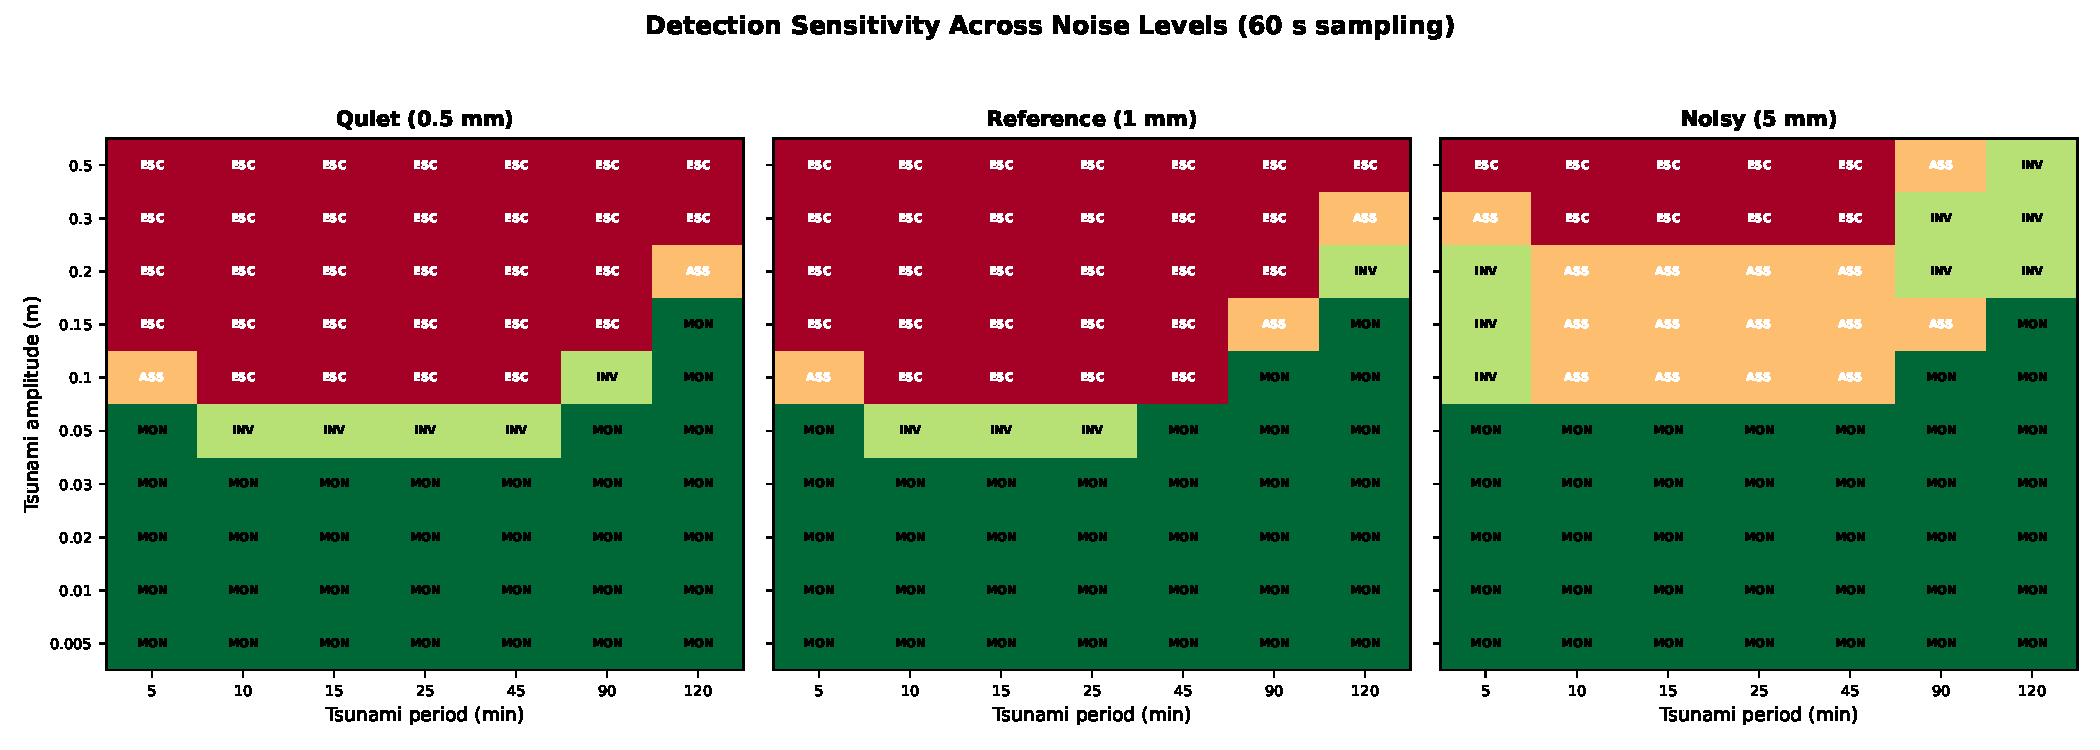
\includegraphics[width=\linewidth]{figures/fig_noise_sensitivity_triptych.pdf}
\caption{Detection sensitivity heatmaps at three ambient noise levels
  (0.5, 1.0, and 5.0\,mm standard deviation) with 60-second sampling.
  Cell labels indicate the maximum FSM state reached (MON = MONITOR,
  INV = INVESTIGATE, ASS = ASSESS, ESC = ESCALATE).  The ESCALATE
  boundary shifts upward by roughly a factor of three at most periods
  between the quietest and noisiest conditions (and beyond the tested
  amplitude range at 90--120\,min periods), demonstrating graceful
  degradation under realistic noise variation.}
\label{fig:noise-triptych}
\end{figure}

\paragraph{Limitations.}
The current implementation has several known constraints. First, the
FSM state and audit log persist to TimescaleDB when a database
connection is available, recovering state on restart; without a
database, the system falls back to in-memory storage where a server
restart clears all state. Second, the system
requires a seismic trigger to leave IDLE; non-seismic tsunamis
(landslide, volcanic) cannot currently activate the pipeline.
Third, the inversion is written against a unit-source database
interface, but the implementation shipped with the release is an
in-memory development store holding caller-supplied synthetic
waveforms, not physics-based propagation solutions.  Running the
inversion at operational quality requires a real propagation database
such as NOAA NCTR, which we did not have access to.  Amplitudes
obtained from the development store are therefore not operationally
meaningful, and none are reported here.
Fourth, during the early stages of a developing event the constraint
stage marks most inversion-dependent checks NOT\_APPLICABLE, and those
are excluded from the aggregate entirely.  At later stages they become
applicable but may still lack their prerequisites: a REQUIRED check in
that position yields INCOMPLETE and the system abstains, while an
OPTIONAL one degrades the outcome to PASS\_WITH\_CONCERNS.  Effective
verification coverage is therefore thin until multiple DART
observations arrive.
Fifth, at the SEISMIC\_ONLY constraint stage the requirement matrix
marks the four inversion-dependent checks (hold-out validation,
sensitivity analysis, DART coverage geometry, waveform fit quality)
NOT\_APPLICABLE and leaves physical consistency as the only REQUIRED
check, so only one check is required to have run.  All four OPTIONAL
checks then report NOT\_EVALUATED with a MISSING prerequisite on the
inputs available at that stage: no earlier assessment is supplied for
the posterior-stability comparison, no component computes a
meteotsunami score, no coastal proxies are attached for the tidal-state
review, and the Rayleigh flag is left unset.  None of the four can
fail, and none contributes evidence either.
The consequence reaches past this stage.  One OPTIONAL check blocked on
a missing prerequisite is enough to degrade the aggregate to
PASS\_WITH\_CONCERNS, and the meteotsunami check alone is OPTIONAL at
all three constraint stages with a prerequisite nothing satisfies, so
PASS is unreachable everywhere rather than only here.  The broader
point is that no component assembles a \texttt{VerificationInput} at
all: the pipeline node that would run these checks reads a
caller-supplied dictionary, and the live worker fail-closes before a
scenario exists to verify.  What this describes is the policy the
checks encode, not behavior observed in a run.
ABSTAIN still activates at this stage: a missing seismic
magnitude leaves that required check without its prerequisite and the
outcome is INCOMPLETE, and a prior scenario whose $M_w$ differs from
the seismic $M_w$ by more than the failure margin returns FAIL.  Both
set \texttt{abstain\_required} and route to ABSTAIN.  The residual
weakness is the thinness of the evidence base at this stage, not the
absence of a gate.
Sixth, the ensemble weights ($\alpha_1{=}0.50$, $\alpha_2{=}0.35$,
$\alpha_3{=}0.15$) and FSM thresholds ($T_1{=}0.35$, $T_2{=}0.60$,
$T_3{=}0.85$) were chosen as design constants based on relative
detector reliability (threshold detection is the most established
technique; the ML component is experimental) and have not been
calibrated against historical events; the system's detection
sensitivity and false-positive rate depend directly on these values.
Seventh, station~46403 (4{,}830\,km) stays below $T_1$ in both the
sliding-window timeline and the full event window
(ensemble~$= 0.311$); the attenuated signal approaches but does not
reach the detection floor, and the tsunami is expected at
${\sim}6.8$\,h, beyond the evaluation window.  NOAA states the same
limitation for the operational 3\,cm criterion: a station "may record
an amplitude of less than 3 cm at the low-amplitude fringe of the main
energy beam for a tsunami that is, in fact, large and
destructive"~\citep[pp.~31--32]{gonzalez2005nthmp}.  This highlights a sensitivity limitation
for far-field stations where tsunami amplitudes approach the detection
floor.  The earliest sliding-window detections per event
(2.7--12.3\,min post-earthquake) correspond to coseismic deformation and seismic
surface-wave arrivals on the BPR, not
the tsunami wave itself; the system does not currently distinguish
seismic from tsunami pressure disturbances.
Eighth, the NDBC historical archive contains 9999.000\,m missing-data
sentinels that, if not filtered, destroy the tidal harmonic fit and cause
threshold-detector saturation on normal data.  The current scripts
filter these values, and the core \texttt{fit\_tidal\_harmonics()}
function uses IRLS with Cauchy weights by default
(Section~\ref{sec:anomaly}); however, this has been tested
only on the five evaluated events.  Explicit sentinel and non-finite
filtering is implemented in both the offline scripts and the live
ingest buffer, but a production system should validate resilience
across a broader range of BPR artifact morphologies (stuck sensors,
partial gaps) and consider alternative weight functions (e.g.,
bisquare) for extreme outlier scenarios.
Ninth, the wavelet detector compares total tsunami-band energies over
windows of unequal length.  \texttt{compute\_wavelet\_energy} returns a
sum of squared detail coefficients, which is an extensive quantity: at
constant signal power it grows in proportion to record length.  The
score forms $E_\text{tsun}/E_\text{base}$ with no length term, while
the calibration window is typically far longer than the scored event
window, so the ratio is dominated by that length difference rather
than by signal power.  Chile station~51407 is the clearest case: the
event window carries $5.1\times$ the calibration window's energy per
sample, yet the calibration record is $102.7\times$ longer, so the raw
ratio is $0.050$ and the score is exactly zero.  Every
\texttt{filter\_degraded} station in the committed artifacts scores
zero on this component for the same reason.  The wavelet component is
therefore suppressed rather than merely noisy, and the reported
detections rest more heavily on the threshold detector than the
nominal weights imply.  We have deliberately not rescaled the score
for this submission, because we measured what rescaling alone does.
Re-running the June 2011 quiet-period evaluation over the same 414
windows with a power-density ratio takes the false-trigger counts from
1/1/0 at $T_1$/$T_2$/$T_3$ to 2/1/1, that is from $0.29$ to $0.57$
false $T_1$ triggers per station-month, and introduces a
$T_3$-level false alarm at station~46408, which rises from $0.802$ to
$0.997$.  The thresholds were chosen against the current suppressed
scale, so the dimensional correction and a recalibration of $T_1$,
$T_2$ and $T_3$ cannot be separated; shipping the first without the
second would trade a known bias for a worse false-escalation rate.
Both belong together in future work.
Tenth, the retrospective evaluation covers five tsunamigenic events
(T\={o}hoku 2011 $M_w$\,9.1, Chile 2010 $M_w$\,8.8, Illapel 2015
$M_w$\,8.3, Iquique 2014 $M_w$\,8.2, and Samoa 2009 $M_w$\,8.1),
all large Pacific earthquakes.  Four are subduction-zone thrust events;
Samoa 2009 is an outer-rise normal-faulting event.
The system has not been validated against smaller-magnitude events
($M_w < 8$), volcanic or landslide-generated tsunamis, or events in
other ocean basins.
Threshold calibration from a broader event catalog remains future work.
Eleventh, the CO-OPS and USGS FDSN ingest connectors are implemented and
unit-tested, but only the DART path is exercised end-to-end.  In the
offline evaluation harness, USGS seismic events drive the FSM trigger from
IDLE; CO-OPS scoring and live multi-source fusion are not exercised.
CO-OPS 6-minute water-level records were retrieved for all five evaluation
events (Figures~\ref{fig:coops-tohoku}--\ref{fig:coops-samoa}), confirming
that tsunami signals are visible at Pacific tide gauges, but the
retrospective detection evaluation uses only DART bottom-pressure records.
That exclusion follows from the archived records rather than from the
sensor class.  The retrieved series are the verified 6-minute water-level
product and sample at exactly 360\,s throughout, whereas the detector
marks any station reaching 150\,s as filter-degraded, that being the
Nyquist limit for its 5-minute high cutoff.  Every retrieved series would
therefore be scored with threshold and wavelet values the detector itself
flags as unreliable, and the QC spike test, which needs consecutive
samples no more than 240\,s apart, would not run at all.  CO-OPS also
publishes a one-minute product that clears both limits, and the live
connector requests it before falling back to the 6-minute one; the
synthetic validation in Section~\ref{sec:eval-physics-sim} samples its
three CO-OPS stations at 60\,s for the same reason.  Re-collecting the
archive at one-minute resolution would make the tide gauges scoreable,
but that product returns only a timestamp and a value, without the sigma
and quality flags carried by the verified 6-minute records, and it would
need per-station calibration baselines the present corpus does not
contain.
Running CO-OPS through scenario inversion and verification remains future
work, as does validating the deployed Kafka worker end-to-end; the worker
currently performs ingest, QC, anomaly scoring, and FSM transitions, and
fail-closes to ABSTAIN at the assessment stages.
Twelfth, the FSM implements a timeout only for the MONITOR state
(returning to IDLE after 12\,h).  The INVESTIGATE and ASSESS states
lack analogous timeouts; a borderline anomaly score that stabilizes
between successive thresholds (e.g., $s \in [T_1, T_2)$) would leave
the FSM in INVESTIGATE indefinitely, blocking acceptance of new
seismic triggers.  Similarly, de-escalation uses the same threshold
values as escalation (zero hysteresis), so scores oscillating near a
boundary can produce rapid state bouncing.  Adding configurable
timeouts and hysteresis offsets for these states is planned.
Thirteenth, the tsunamigenic zone filter used in the seismic trigger
(Section~\ref{sec:fsm}) currently covers a test subset of subduction
zones; complete zone definitions aligned with PTWC operational
boundaries are required for production use.
Fourteenth, the synthetic simulation module uses a constant ocean
depth ($h = 4000$\,m) and flat-Earth $1/\sqrt{r}$ spreading, ignoring
bathymetric refraction, focusing, and spherical-Earth geometrical
spreading effects that can alter amplitudes by factors of 2--5 at
transoceanic distances.  Green's Law shoaling is applied down to
10--20\,m depth (CO-OPS station locations), where nonlinear effects
and bottom friction invalidate the linear approximation.  The
cos$^2$ azimuthal directivity pattern is an ad-hoc parameterization,
not derived from a published tsunami directivity model.
The simulation includes multi-frequency spectra, frequency-dependent
coda decay, and N-wave polarity (Section~\ref{sec:eval-physics-sim}),
but near-field amplitude matching (e.g., DART~21418 at 560\,km during
the 2011 Tohoku event) requires a finite-fault Okada model beyond the
parametric scope, and the Wells \& Coppersmith regressions break down
above $M_w$~8.5.
These simplifications are acceptable for software verification
purposes but are not representative of operational tsunami modeling.
Fifteenth, the anomaly-score-driven escalation path depends on
ocean observations: the ensemble score that advances the FSM through
INVESTIGATE and ASSESS is computed from water-level data, and the
ASSESS-to-ESCALATE seismic override requires DART event-mode
confirmation.  To complement this, the FSM also implements a
seismic-only escalation path
aligned with PTWC/JMA operational practice: large shallow earthquakes
($M \geq 7.5$, depth $< 100$\,km) in tsunamigenic zones trigger
immediate escalation to human review without requiring ocean data.
DART observations, when available, refine the assessment during the
15--30 minute window between seismic detection and tsunami wave arrival.
This two-phase architecture mirrors the standard operational model
where initial warnings are seismic-based and subsequent bulletins
incorporate sea-level confirmation~\citep{bernard2015evolution}.
Sixteenth, the FSM advances based on the maximum single-station
ensemble score; no multi-station spatial coherence criterion gates
the escalation decision.  The data-coverage verification check
(Section~\ref{sec:verification}) requires $\geq 2$ stations post-hoc,
but this is a verification constraint, not a detection gate, so the
FSM can reach ESCALATE from a single station's score.
Seventeenth, the propagation module computes frequency-dependent
dispersion corrections (Section~\ref{sec:eval-physics-sim}) but
these are not applied to the arrival-time estimates used by the
verification agent's travel-time check; arrival times assume the
non-dispersive shallow-water speed $c = \sqrt{gH}$.  For
transoceanic paths ($>$5{,}000\,km) dispersion can delay dominant
tsunami periods by tens of minutes relative to the
leading wave~\citep{kajiura1963leading}.
Eighteenth, the coastal amplitude proxies produced by the scenario
inversion agent use the deep-ocean NNLS waveform amplitudes directly
without applying Green's Law shoaling amplification
($A_\text{coast} \propto (h_\text{deep}/h_\text{shore})^{1/4}$).
The simulation module applies Green's Law (Section~\ref{sec:eval-physics-sim}),
but the inversion pipeline does not, so coastal amplitude estimates
from the inversion are underestimates.
Nineteenth, the BOCPD changepoint detector assumes i.i.d.\ Gaussian
observations within each run length~\citep{adams2007bayesian}.
Bandpass-filtered ocean pressure residuals exhibit short-range
autocorrelation that violates this assumption, potentially inflating
the false changepoint rate.  Alternative formulations incorporating
autoregressive observation models~(e.g., AR(1) within-segment likelihood)
would improve statistical validity but increase computational cost.

\paragraph{Future work.}
Planned extensions include a multi-event FSM for concurrent
tracking of independent seismic triggers; adaptive threshold
calibration from historical DART event archives; integration with
the NOAA CO-OPS one-minute tsunami product; and Kubernetes
deployment for horizontal scaling during multi-event scenarios.
Additional read-only LangGraph advisory nodes (e.g., data quality
explanation, SOP compliance checking) are architecturally viable under
the bounded autonomy design but deferred pending calibration and
evaluation of the core synthesis graph.

% ============================================================
%  8. Broader Impacts
% ============================================================

\section{Broader Impacts}

This work augments tsunami situational awareness for
duty scientists. Faster and more transparent data integration
supports the duty scientists whose judgments feed the official
warning process.  The system itself issues nothing and reaches no
member of the public.

The system explicitly does \emph{not} replace or
interfere with NOAA's official warning systems. All emitted assessment
reports carry non-authoritative disclaimers. The Human Review
Gate blocks autonomous public communication. The bounded
agency model and machine-readable permission matrix document the
capability envelope of each component, and the append-only audit trail
supports independent review of FSM transitions, verification outcomes,
and human review decisions; complete raw-to-output
\texttt{input\_refs} provenance is not yet exposed end to end.

Potential risks include over-reliance on the system's outputs if
duty scientists do not maintain independent judgment, and
misinterpretation of \texttt{APPROVED\_INTERNAL} as an official
product. Both risks are mitigated by the disclaimer mechanism and
the system's framing as a situational awareness tool, not a warning
system. The code and design documents are public to allow
independent scrutiny.
False negatives pose a distinct risk: if the ensemble score remains
below $T_1$ during a genuine event (e.g., due to DART station
outage or an atypical source), the system's quiescent display may
reinforce inaction.  Operator training must emphasize that the
system supplements, not substitutes, independent seismic and
tide-gauge monitoring.
The seismic trigger requirement (see Limitations) excludes
non-seismic tsunamis; this constraint must be clearly communicated
to operators.

% ============================================================
%  9. Conclusion
% ============================================================

\section{Conclusion}

We have presented a bounded agentic AI framework for near-real-time
ocean hazard assessment that processes observations through a structured pipeline integrating
DART bottom-pressure records, CO-OPS water-level observations,
and USGS seismic event feeds for tsunami situational awareness. The framework's key properties are: a
deterministic FSM orchestrator with bidirectional de-escalation;
an ensemble anomaly detector combining three core signal analysis
methods with an optional ML component; NNLS scenario inversion with bootstrap uncertainty
quantification; a fail-closed verification layer with an explicit
ABSTAIN output; an append-only audit trail with SHA-256 hashing at ingest
boundaries (end-to-end \texttt{input\_refs} provenance to the final assessment
is still being wired); a bounded LLM advisory layer whose operator
narratives are stored separately from the deterministic report of
record and dropped on failure or guardrail violation; and a mandatory Human Review Gate
for all full assessments.  Retrospective replay on five Pacific tsunamigenic
earthquakes ($M_w$\,8.1--9.1: T\={o}hoku 2011, Chile 2010,
Illapel 2015, Iquique 2014, and Samoa 2009) shows that
the ensemble detector exceeds the fixed operating-point
thresholds at event-mode DART stations for each event,
spanning subduction-zone thrust
and outer-rise normal-faulting mechanisms; the earliest
detections reflect coseismic pressure perturbations rather than
confirmed tsunami wave arrivals.  Systematic threshold
calibration from a broader event catalog remains necessary before
operational deployment.  The published implementation and
structured audit trail provide a foundation for community-driven
calibration and extension to additional ocean hazard types.

% ============================================================
%  References
% ============================================================

\bibliographystyle{unsrtnat}
\bibliography{references}

% ============================================================
%  Appendix - UML Diagrams
% ============================================================

\newpage
\appendix
\renewcommand{\thefigure}{A.\arabic{figure}}
\setcounter{figure}{0}
\section{UML Diagrams}
\label{sec:appendix-uml}

This appendix presents the full UML diagrams for the system
architecture, generated from the draw.io source files in
\texttt{paper/drawio/}.

\begin{figure}[ht!]
\centering
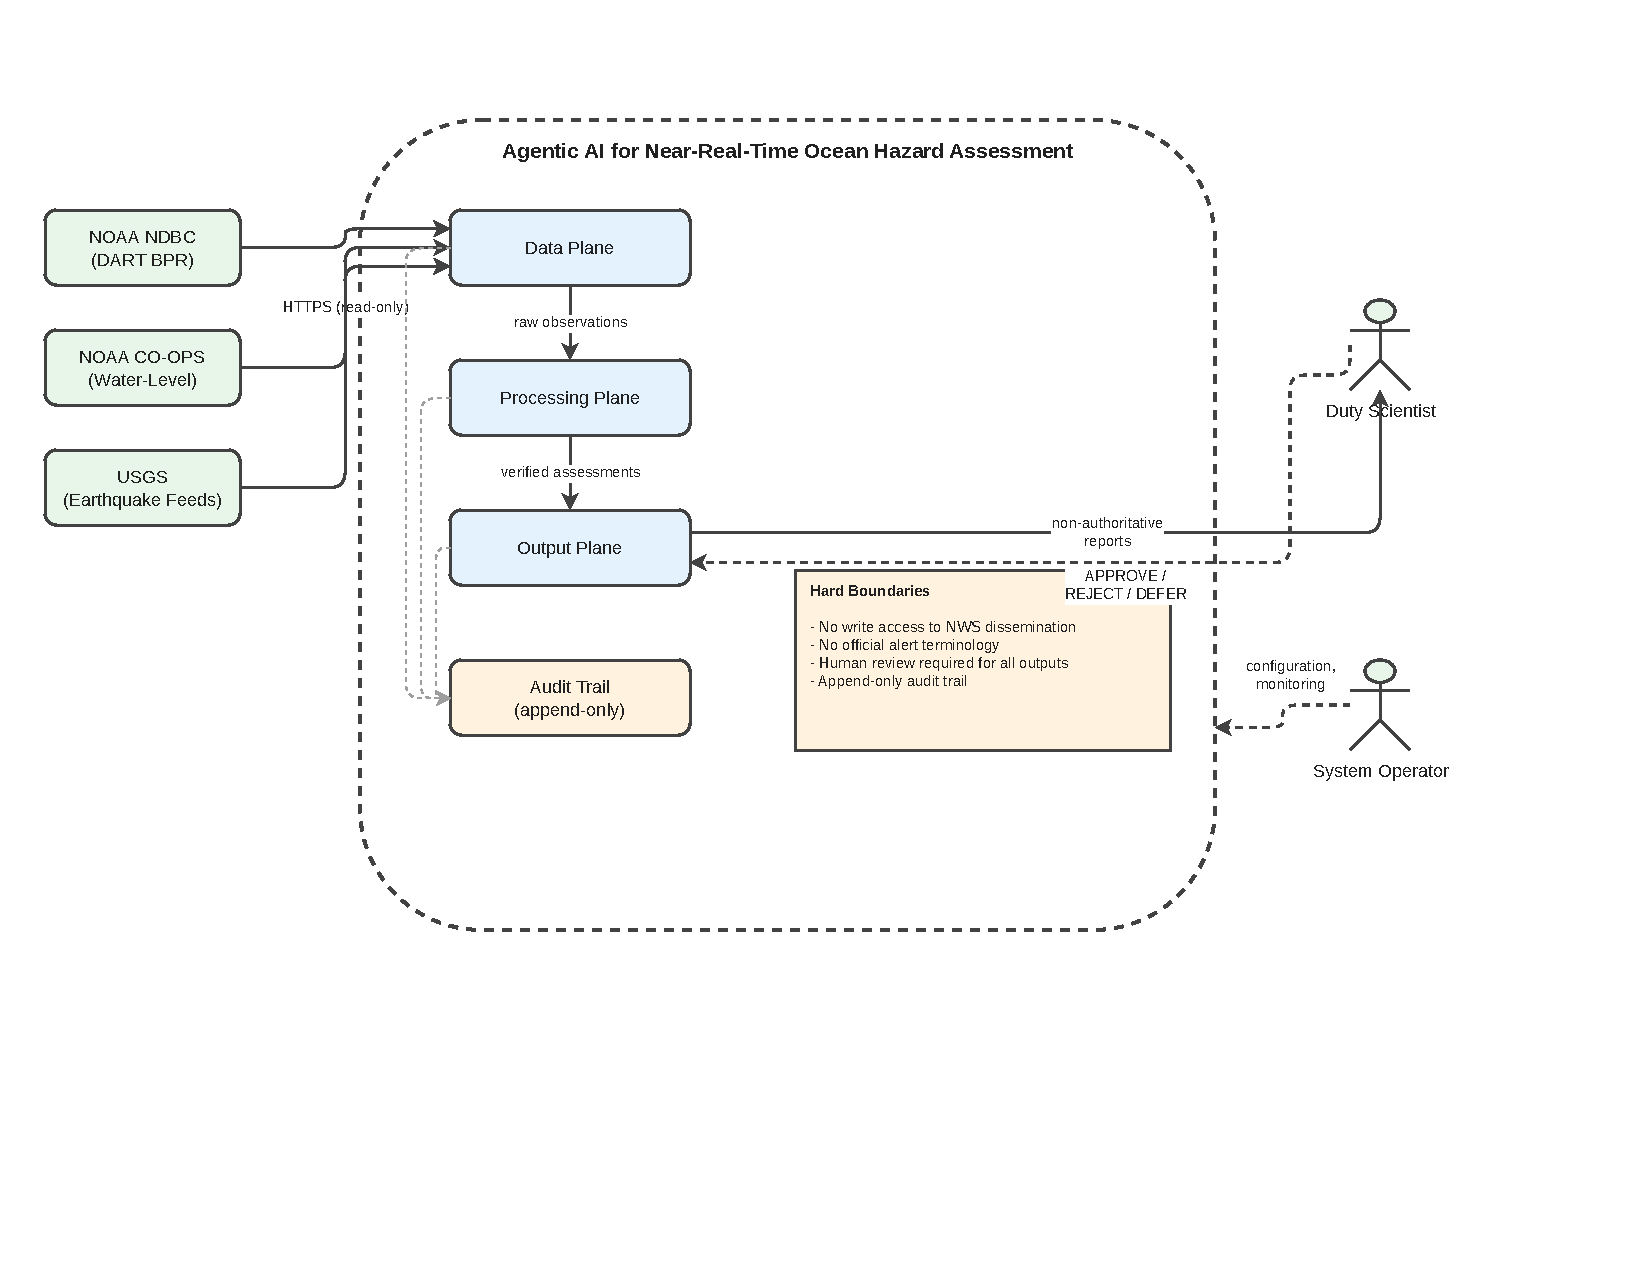
\includegraphics[width=\textwidth]{figures/system-context.pdf}
\caption{System context diagram. External actors (Duty Scientist,
  System Operator) and read-only data feeds (NOAA NDBC, NOAA CO-OPS,
  USGS) interact with the system boundary. Hard constraints include
  no write access to NWS dissemination, no use of official alert
  terminology, and required human review for all distributable
  outputs.}
\label{fig:uml-system-context}
\end{figure}

\begin{figure}[ht!]
\centering
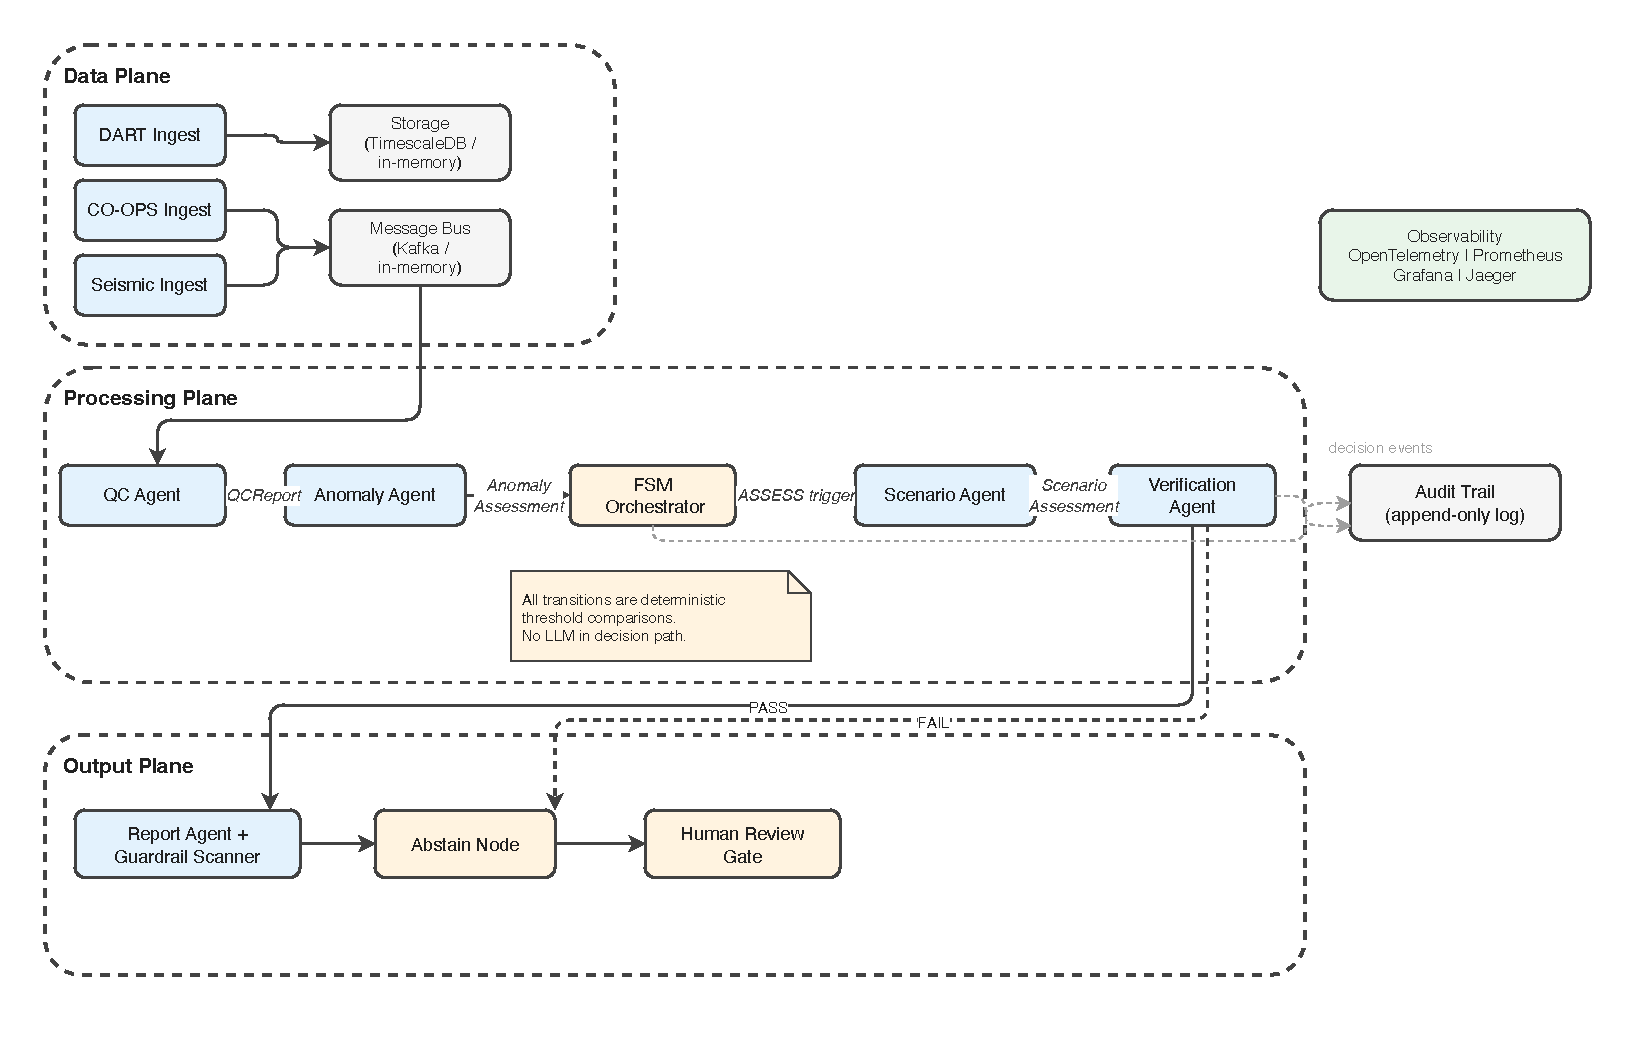
\includegraphics[width=\textwidth]{figures/component-diagram.pdf}
\caption{Component diagram showing the internal structure of the
  system. The Data Plane ingests from three external feeds into
  in-memory stores (the deployed worker consumes Kafka and persists
  raw observations and audit records to TimescaleDB when configured). The Processing Plane contains the
  QC, Anomaly, Scenario, and Verification agents orchestrated by
  the deterministic FSM. The Output Plane includes the Report Agent,
  alert-language guardrail scanner, Abstain Node, and Human Review
  Gate. Observability is provided by the Telemetry Tracing module
  (OpenTelemetry), Prometheus, Grafana, and Jaeger.}
\label{fig:uml-component}
\end{figure}

\begin{figure}[ht!]
\centering
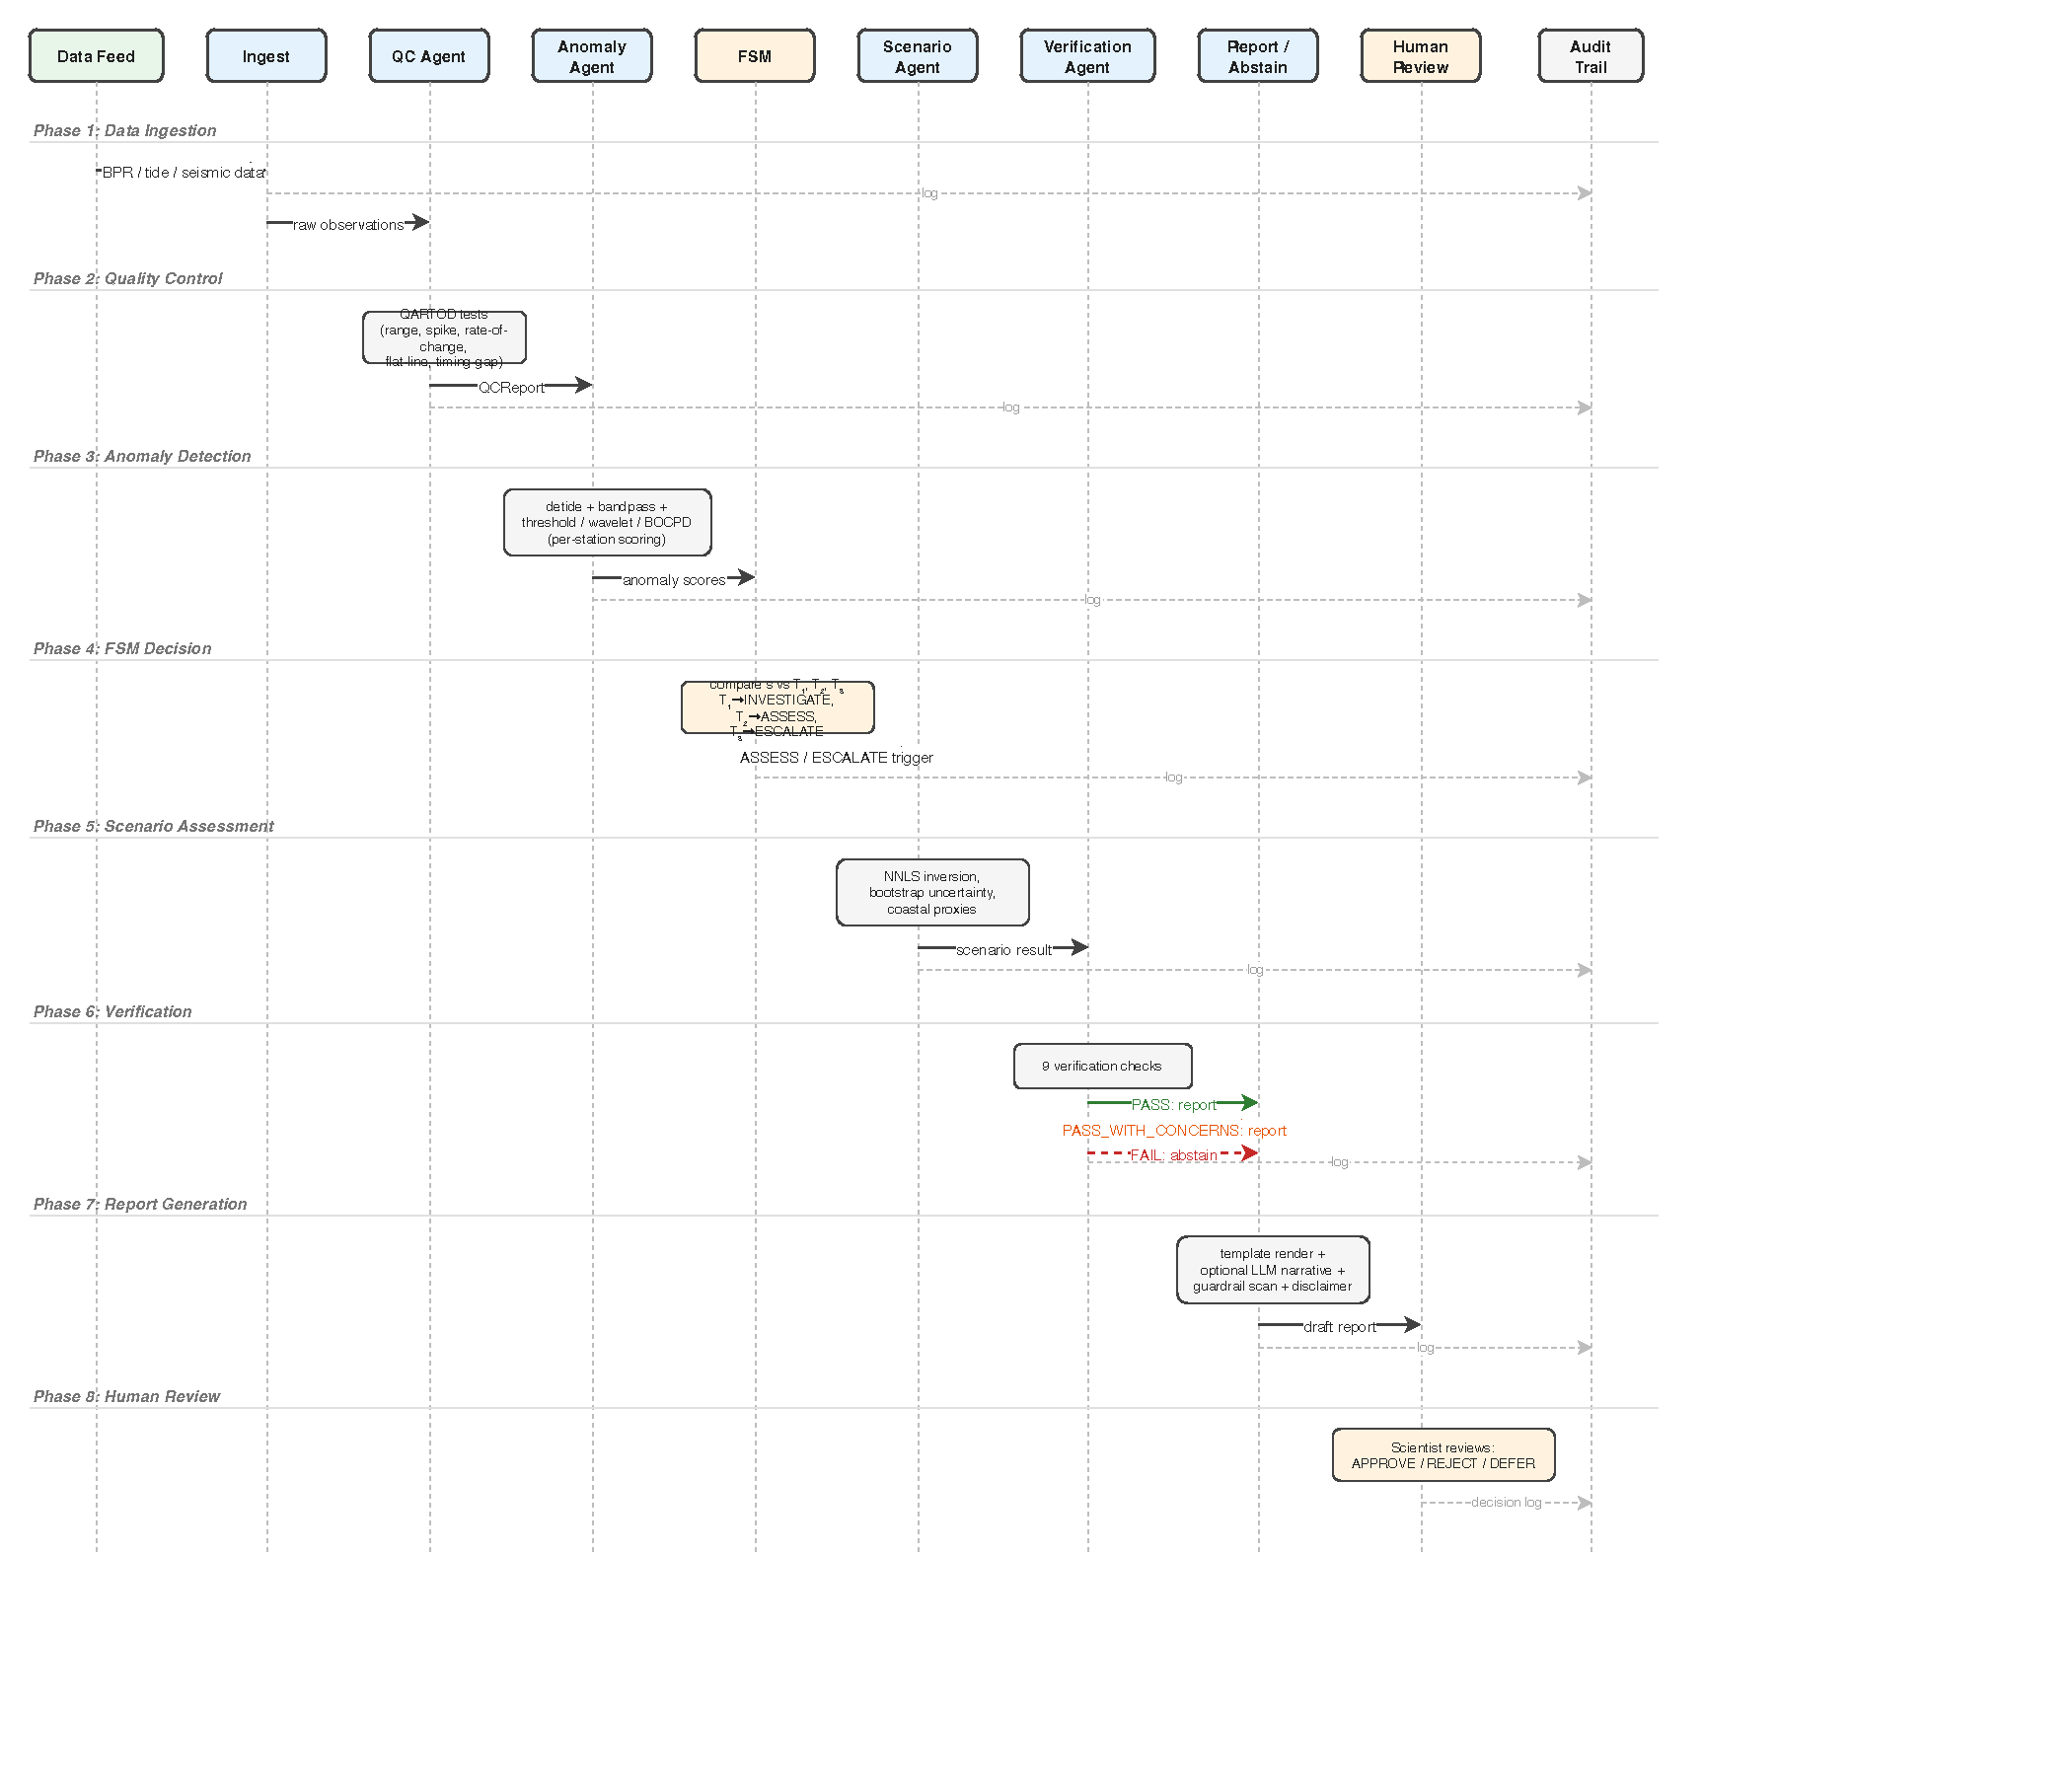
\includegraphics[width=\textwidth]{figures/pipeline-sequence.pdf}
\caption{Pipeline sequence diagram for a tsunami event assessment.
  The flow proceeds through data ingestion, five QARTOD quality-control
  tests (range, spike, rate-of-change, flat-line, timing-gap), ensemble
  anomaly detection, deterministic FSM transition (thresholds
  $T_1 \to$ INVESTIGATE, $T_2 \to$ ASSESS, $T_3 \to$ ESCALATE),
  NNLS scenario inversion (triggered by ASSESS or ESCALATE), nine-check
  verification (with PASS, PASS\_WITH\_CONCERNS, and FAIL/ABSTAIN paths),
  report generation (template rendering, optional LLM narrative, guardrail
  scanning), and human review. In the full assessment flow, every step
  writes to the append-only audit trail (in-memory, with optional
  TimescaleDB persistence when a database
  connection is available).}
\label{fig:uml-sequence}
\end{figure}

\begin{figure}[ht!]
\centering
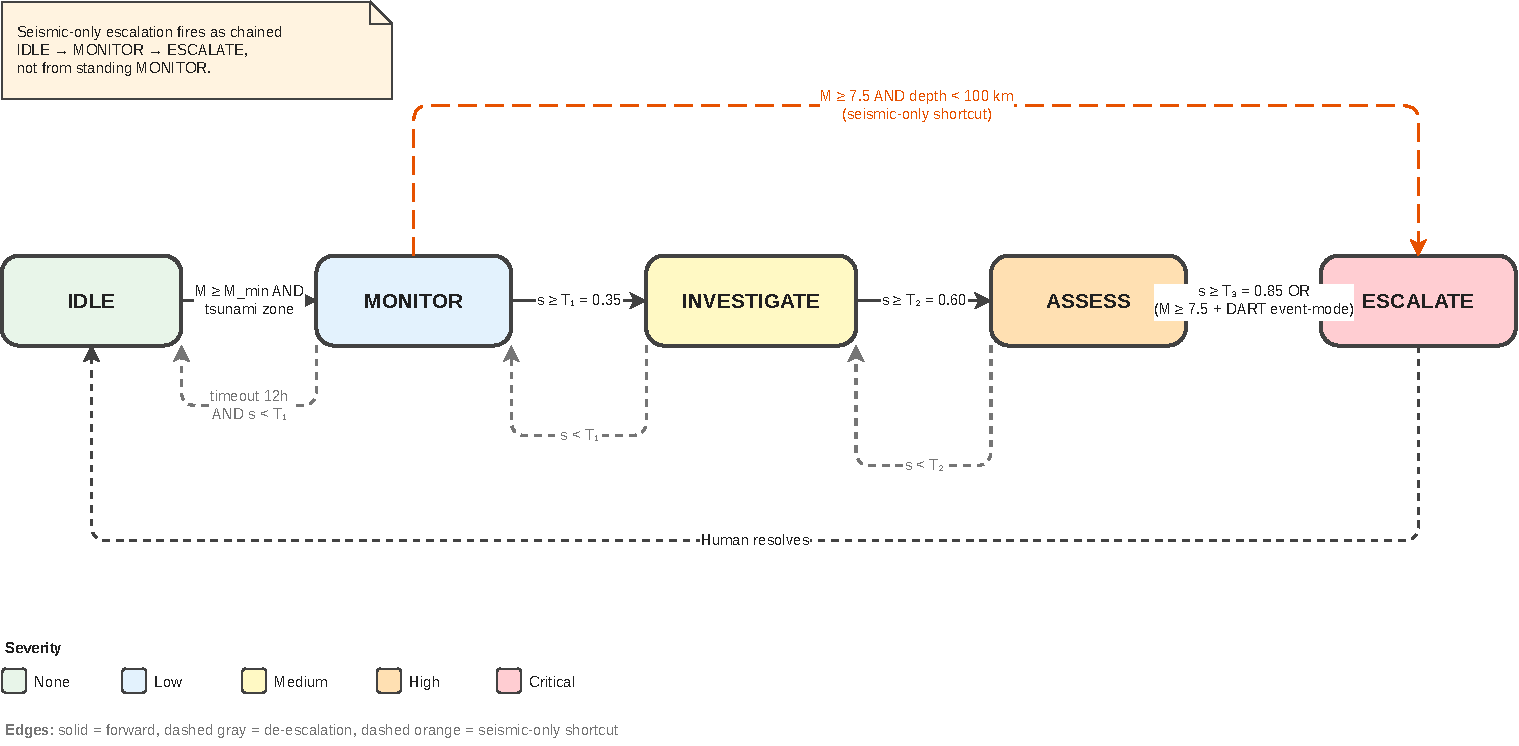
\includegraphics[width=\textwidth]{figures/fsm-states.pdf}
\caption{FSM state machine diagram. Five states (IDLE, MONITOR,
  INVESTIGATE, ASSESS, ESCALATE) with deterministic threshold-based
  forward transitions ($T_1{=}0.35$, $T_2{=}0.60$, $T_3{=}0.85$),
  bidirectional de-escalation paths, a 12-hour timeout rule for
  MONITOR~$\to$~IDLE, and a seismic override shortcut
  ($M \geq 7.5$ with DART event-mode activation).}
\label{fig:uml-fsm}
\end{figure}

\begin{figure}[ht!]
\centering
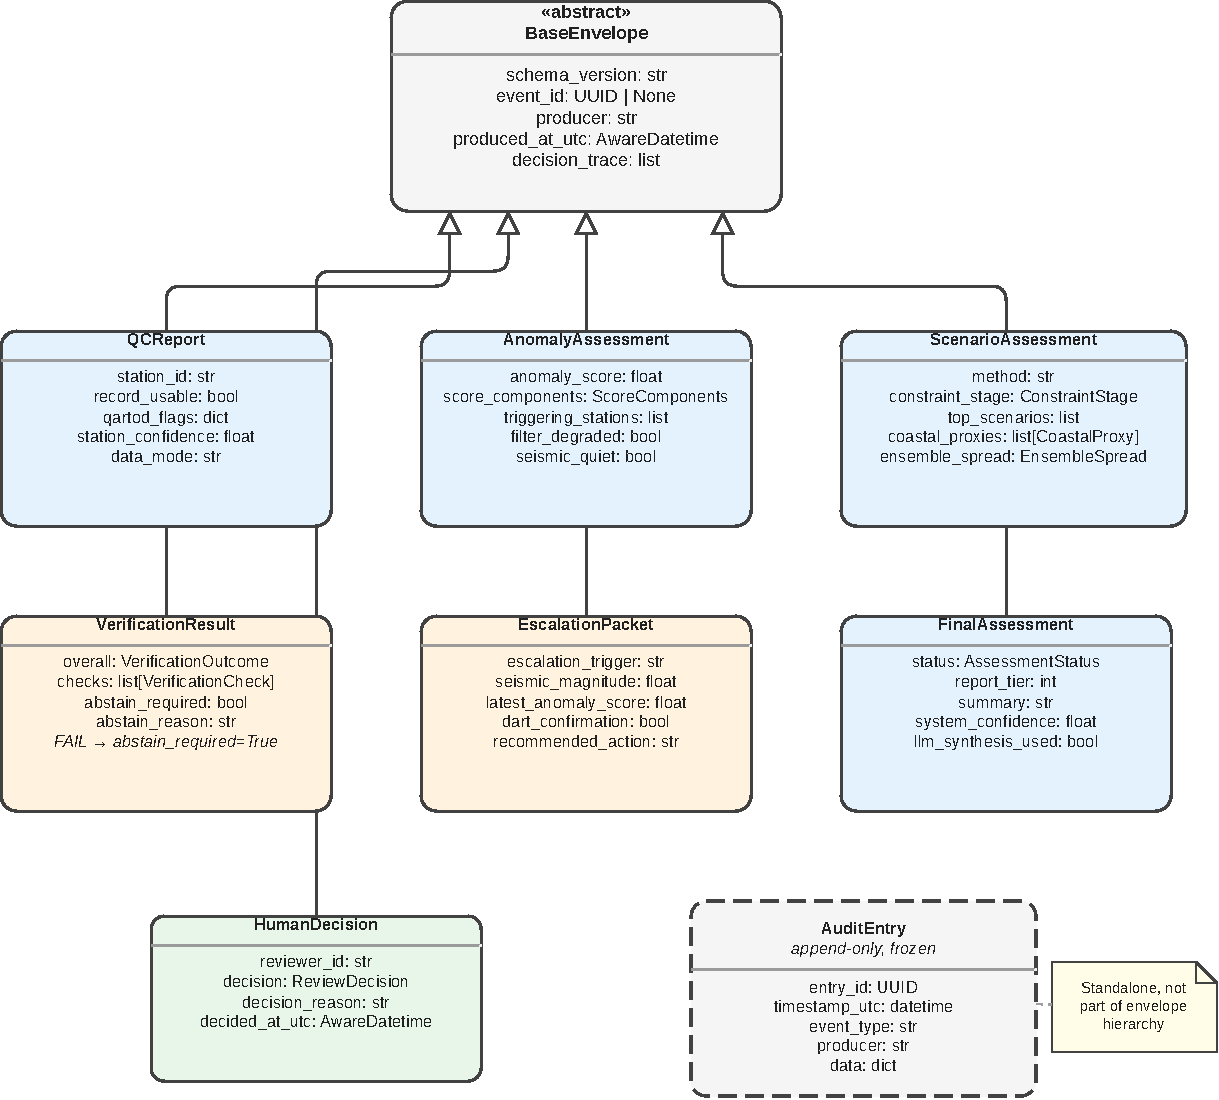
\includegraphics[width=\textwidth]{figures/data-schemas.pdf}
\caption{Handoff schema class diagram (Pydantic v2,
  \texttt{extra="forbid"}). All inter-agent messages inherit from
  \texttt{BaseEnvelope}; the diagram shows its schema version, event
  ID, producer identity, UTC timestamp, and decision trace (the full
  schema also carries a handoff ID, input references with SHA-256
  hashes, and code/model versions).
  Subtypes include \texttt{QCReport}, \texttt{AnomalyAssessment},
  \texttt{ScenarioAssessment}, \texttt{VerificationResult},
  \texttt{EscalationPacket}, \texttt{FinalAssessment}, and
  \texttt{HumanDecision}. The standalone \texttt{AuditEntry} schema
  (append-only, frozen) is also shown.}
\label{fig:uml-schemas}
\end{figure}

\begin{figure}[ht!]
\centering
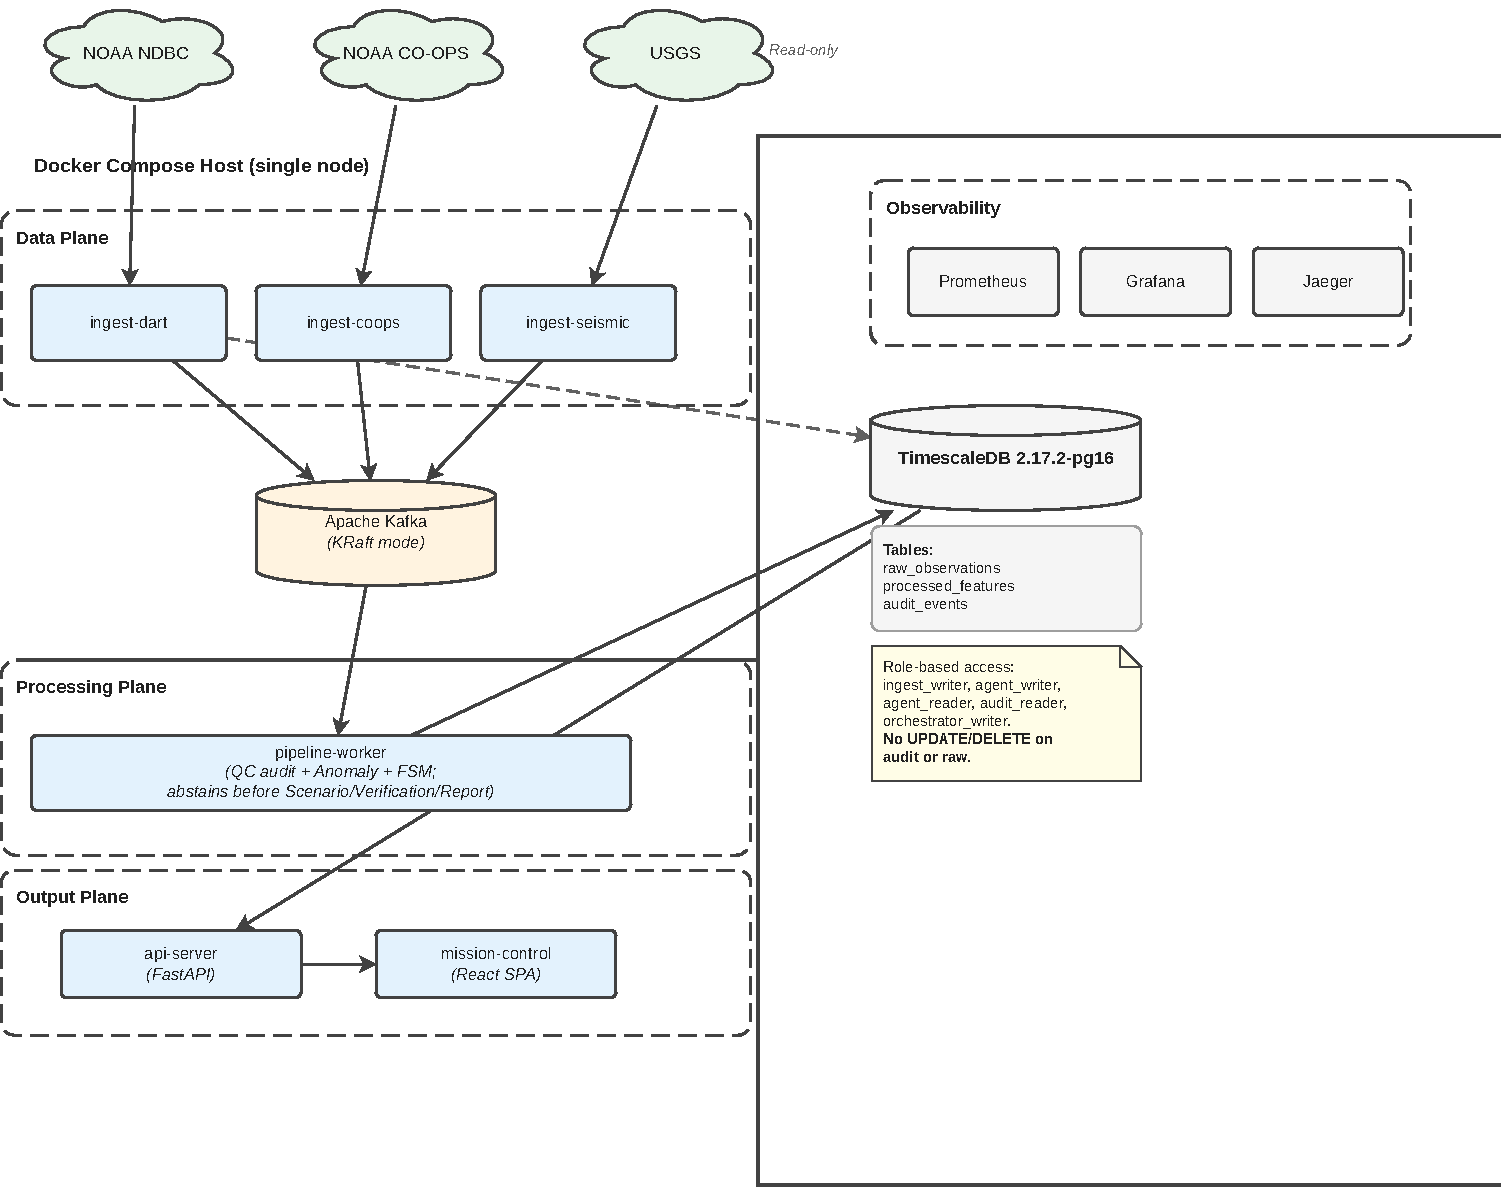
\includegraphics[width=\textwidth]{figures/deployment-diagram.pdf}
\caption{Deployment diagram for the single-node Docker Compose stack.
  Services include three ingest containers (Data Plane), a single
  pipeline-worker container (Processing Plane), API server and
  Mission Control BFF with React SPA (Output Plane), TimescaleDB
  2.17-pg16 with role-based access control, Apache Kafka in KRaft
  mode (no ZooKeeper), and an observability stack (Prometheus,
  Grafana, Jaeger).}
\label{fig:uml-deployment}
\end{figure}

\begin{figure}[ht!]
\centering
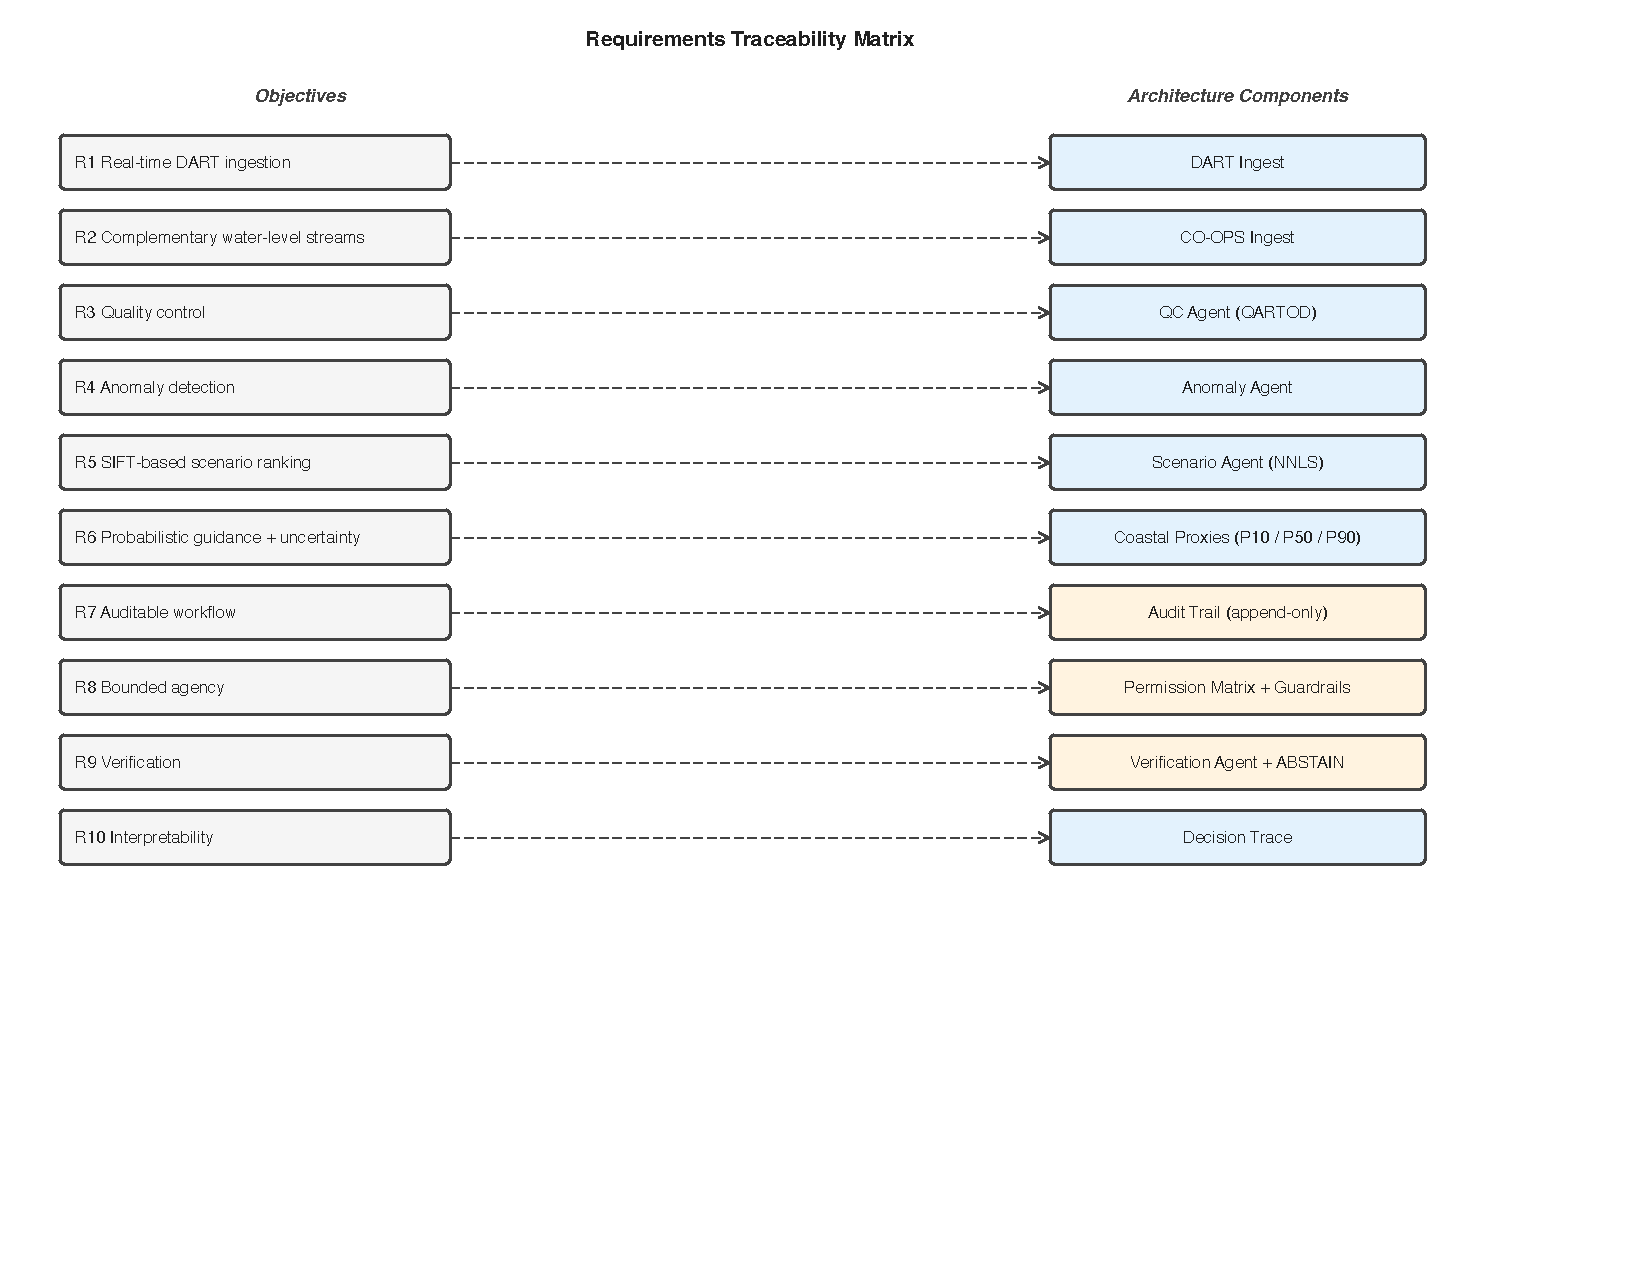
\includegraphics[width=\textwidth]{figures/requirements-traceability.pdf}
\caption{Requirements traceability diagram mapping the ten abstract
  objectives (R1--R10) to architectural components. Each requirement
  is satisfied by a specific component: DART Ingest (R1), CO-OPS
  Ingest (R2), QC Agent (R3), Anomaly Agent (R4), Scenario Agent
  (R5), Coastal Proxies (R6), Audit Trail (R7), Permission Matrix
  and Guardrails (R8), Verification Agent and ABSTAIN (R9), and
  Decision Trace (R10). The two components shown against R8, bounded
  autonomy, contribute differently: the guardrail scanner blocks
  emission, while the permission matrix declares the capability
  envelope and is evaluated only when queried.}
\label{fig:uml-traceability}
\end{figure}

\begin{figure}[ht!]
\centering
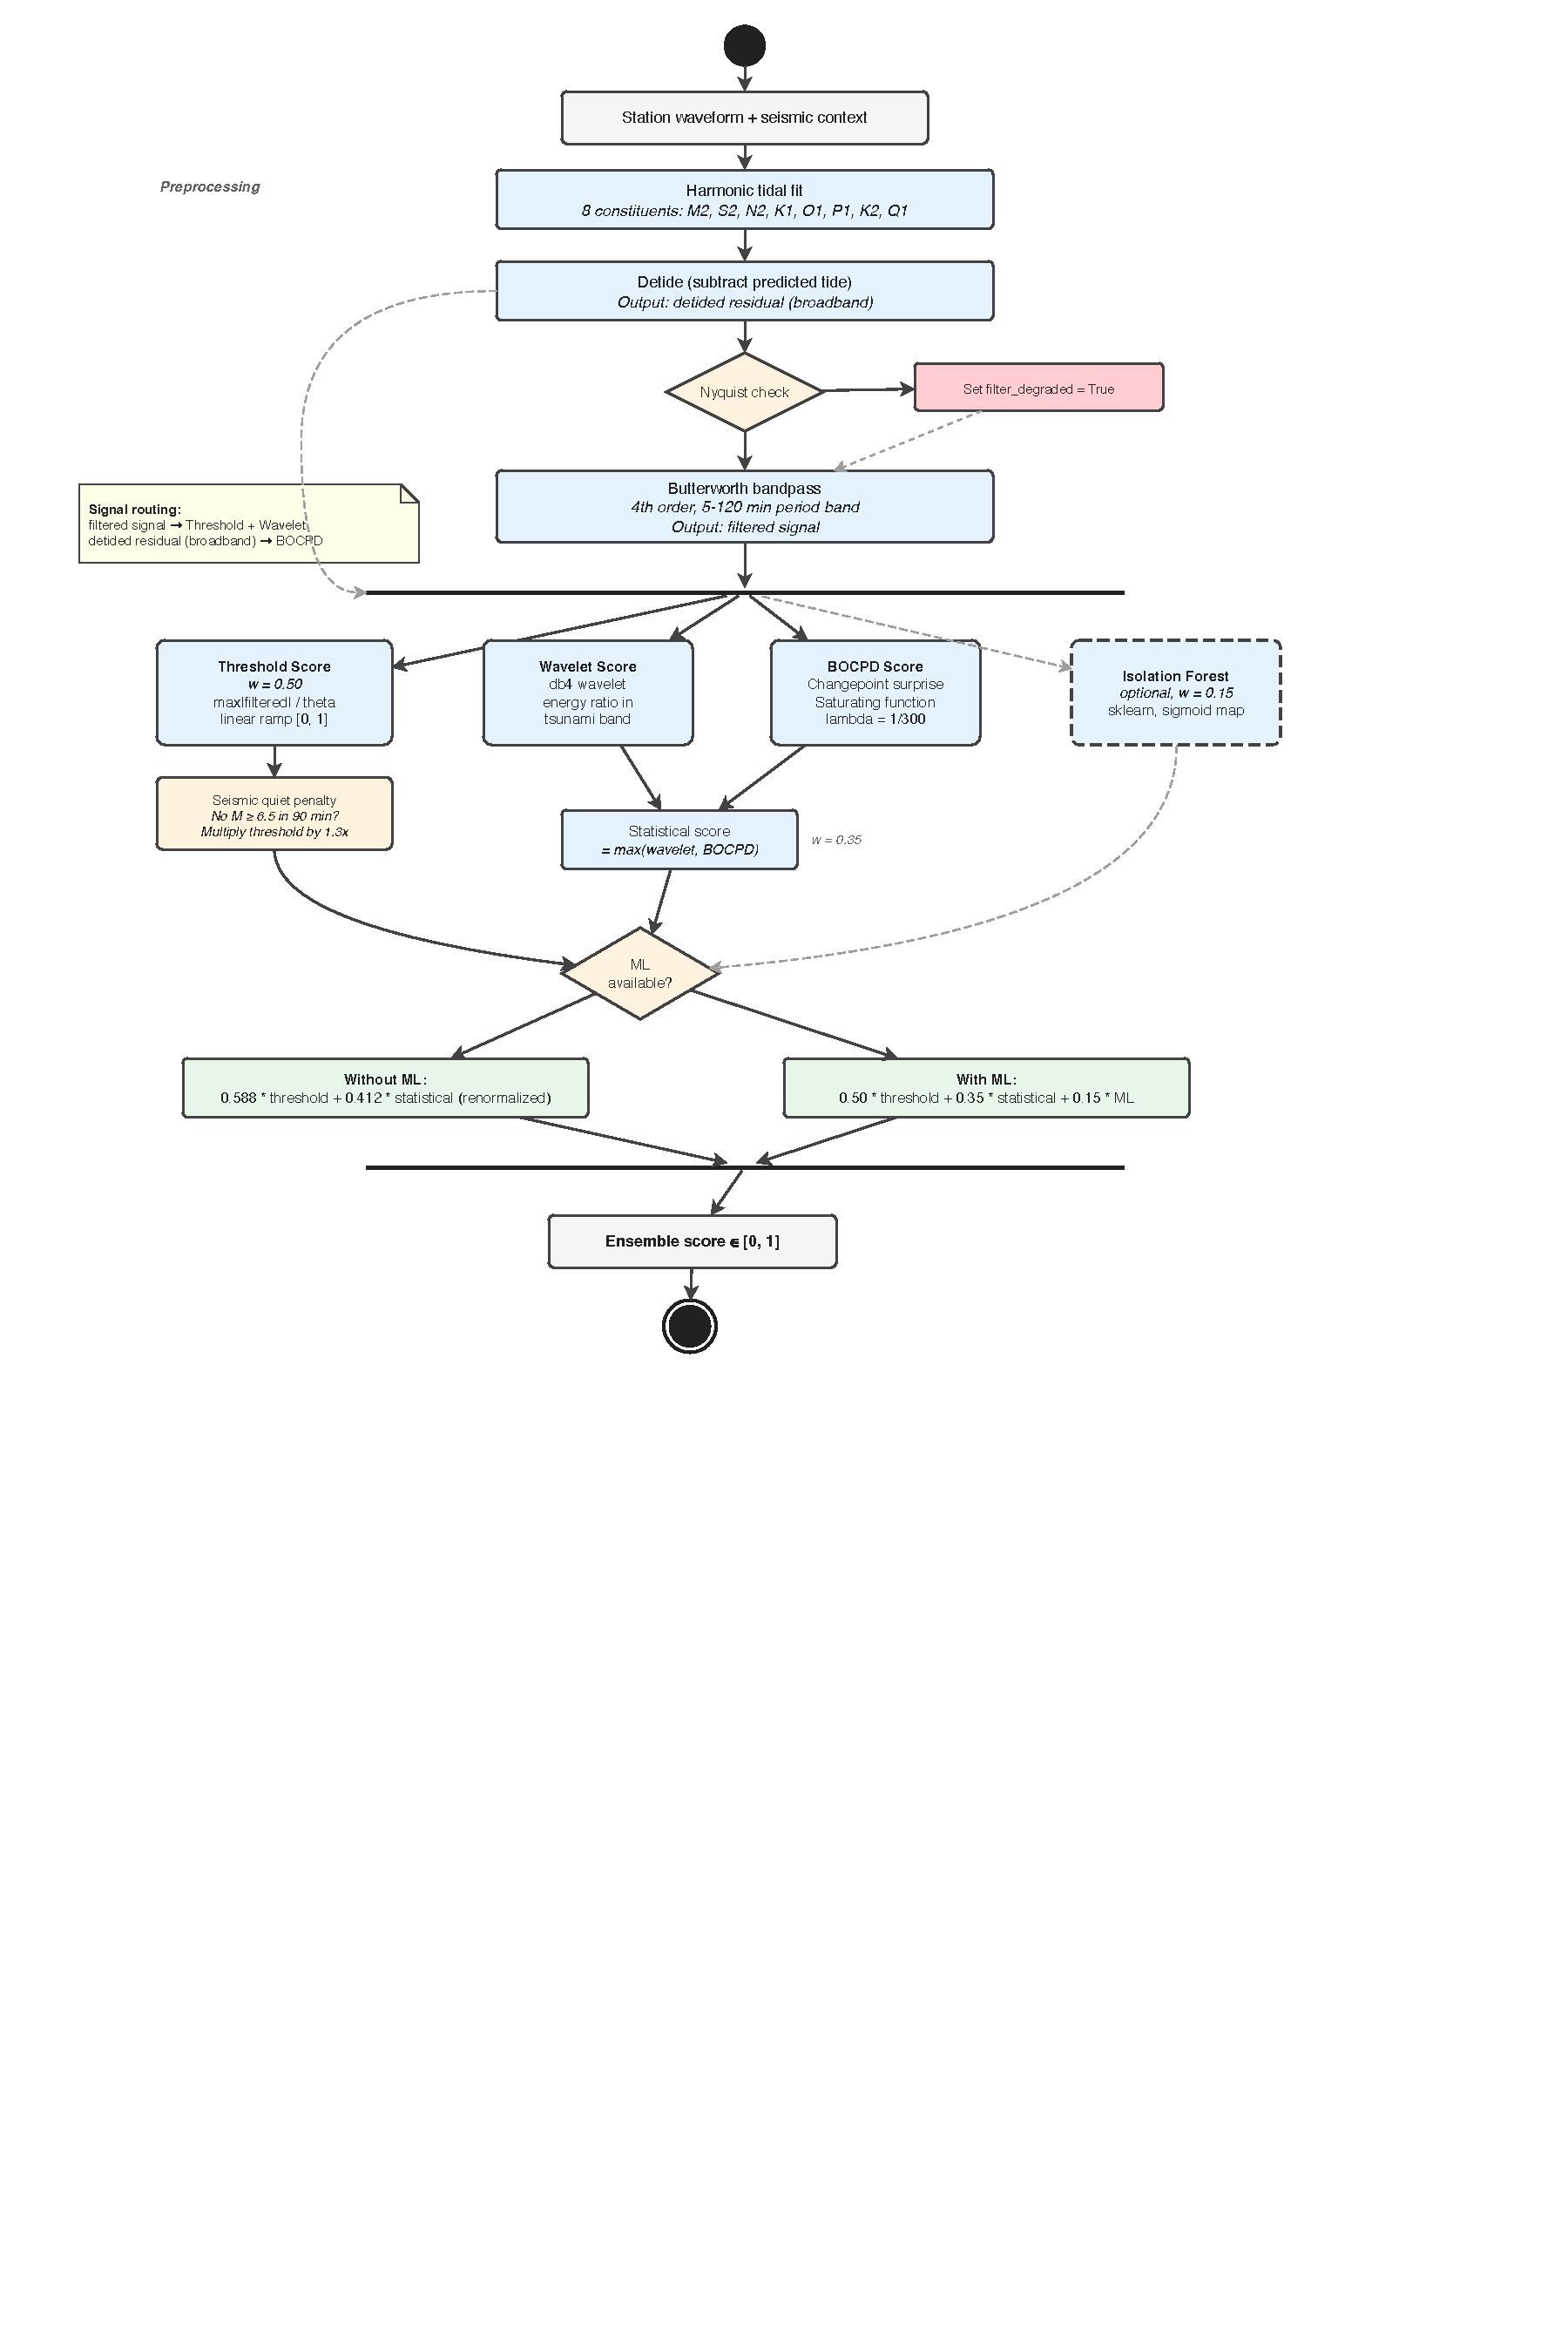
\includegraphics[width=\textwidth]{figures/anomaly-ensemble-activity.pdf}
\caption{Anomaly ensemble activity diagram. Preprocessing (detide,
  bandpass filter, Nyquist check) feeds a parallel fork into four
  detection paths: threshold exceedance ($w{=}0.50$), wavelet energy
  ratio, Bayesian Online Changepoint Detection (BOCPD), and an
  optional Isolation Forest ($w{=}0.15$). The wavelet and BOCPD
  scores are combined via $\max(\cdot)$ into a single statistical
  branch ($w{=}0.35$). Weighted fusion with ML-available and
  ML-absent branches produces the composite anomaly score; when the
  Isolation Forest is unavailable, weights renormalize to
  $(0.588, 0.412)$.}
\label{fig:uml-anomaly-ensemble}
\end{figure}

\begin{figure}[ht!]
\centering
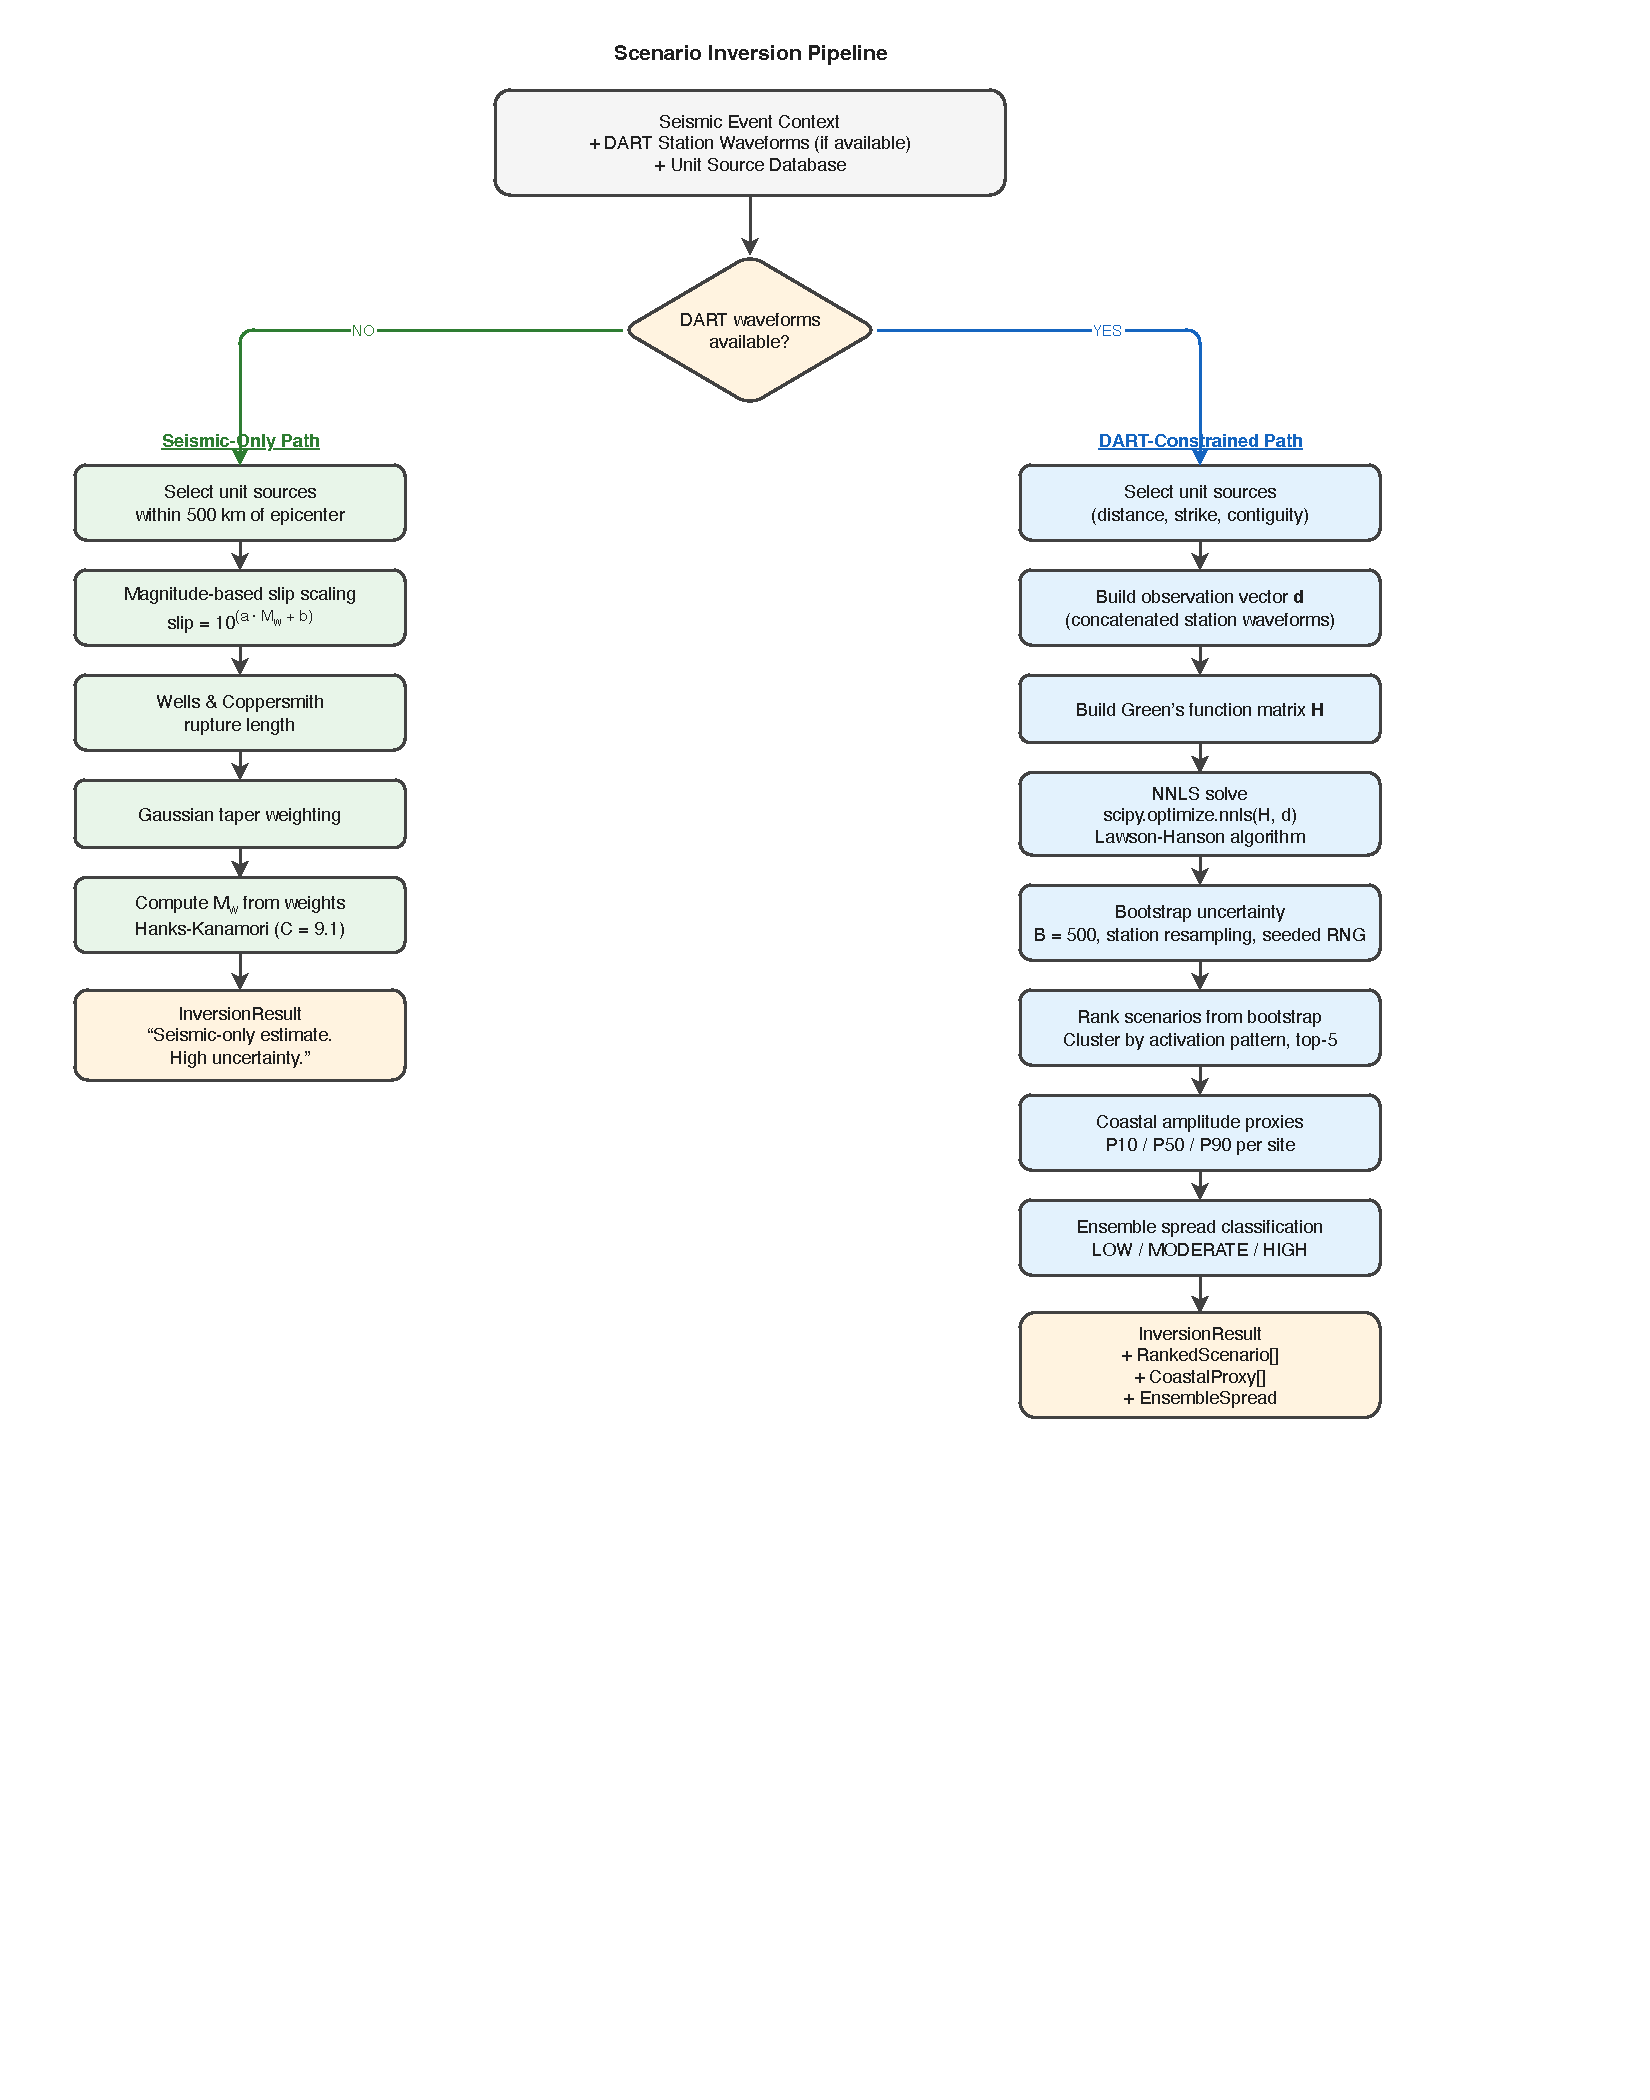
\includegraphics[width=\textwidth,height=0.85\textheight,keepaspectratio]{figures/scenario-inversion-activity.pdf}
\caption{Scenario inversion activity diagram. DART-constrained and
  seismic-only paths diverge at the constraint stage. Unit source
  selection, Green's function matrix assembly, NNLS inversion,
  moment magnitude calculation, bootstrap uncertainty estimation
  (500 iterations), coastal amplitude proxies (P10/P50/P90), and
  ensemble spread computation produce ranked scenarios.}
\label{fig:uml-scenario-inversion}
\end{figure}

\begin{figure}[ht!]
\centering
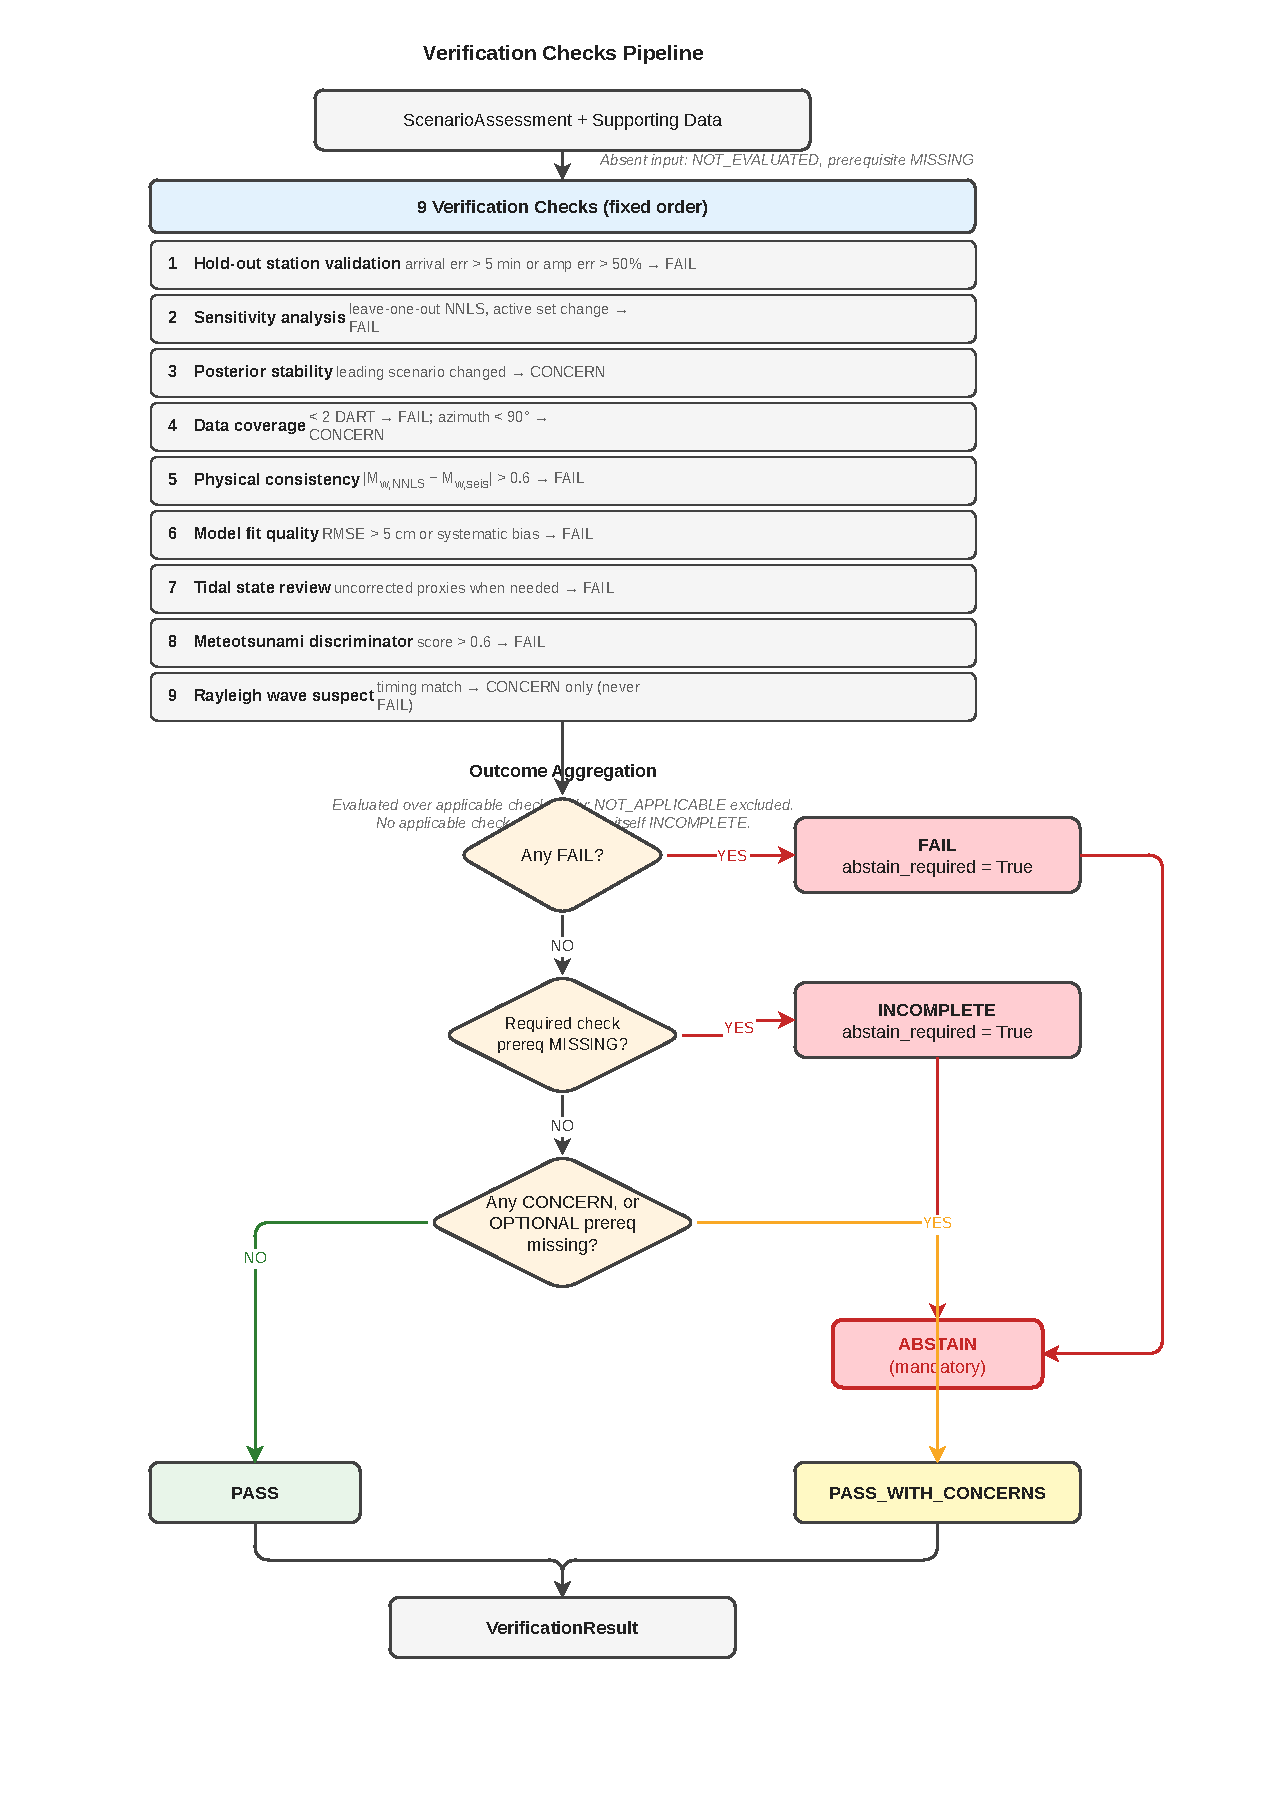
\includegraphics[width=\textwidth,height=0.85\textheight,keepaspectratio]{figures/verification-checks-activity.pdf}
\caption{Verification checks activity diagram. Nine verification
  checks (hold-out validation, sensitivity analysis, posterior stability,
  data coverage, physical consistency, model fit, tidal state,
  meteotsunami screening, and Rayleigh wave suspect) with their
  specific thresholds. A check whose input is absent returns
  NOT\_EVALUATED with its prerequisite marked MISSING. Outcome
  aggregation routes both FAIL and INCOMPLETE verdicts to the ABSTAIN
  path.}
\label{fig:uml-verification-checks}
\end{figure}

\begin{figure}[ht!]
\centering
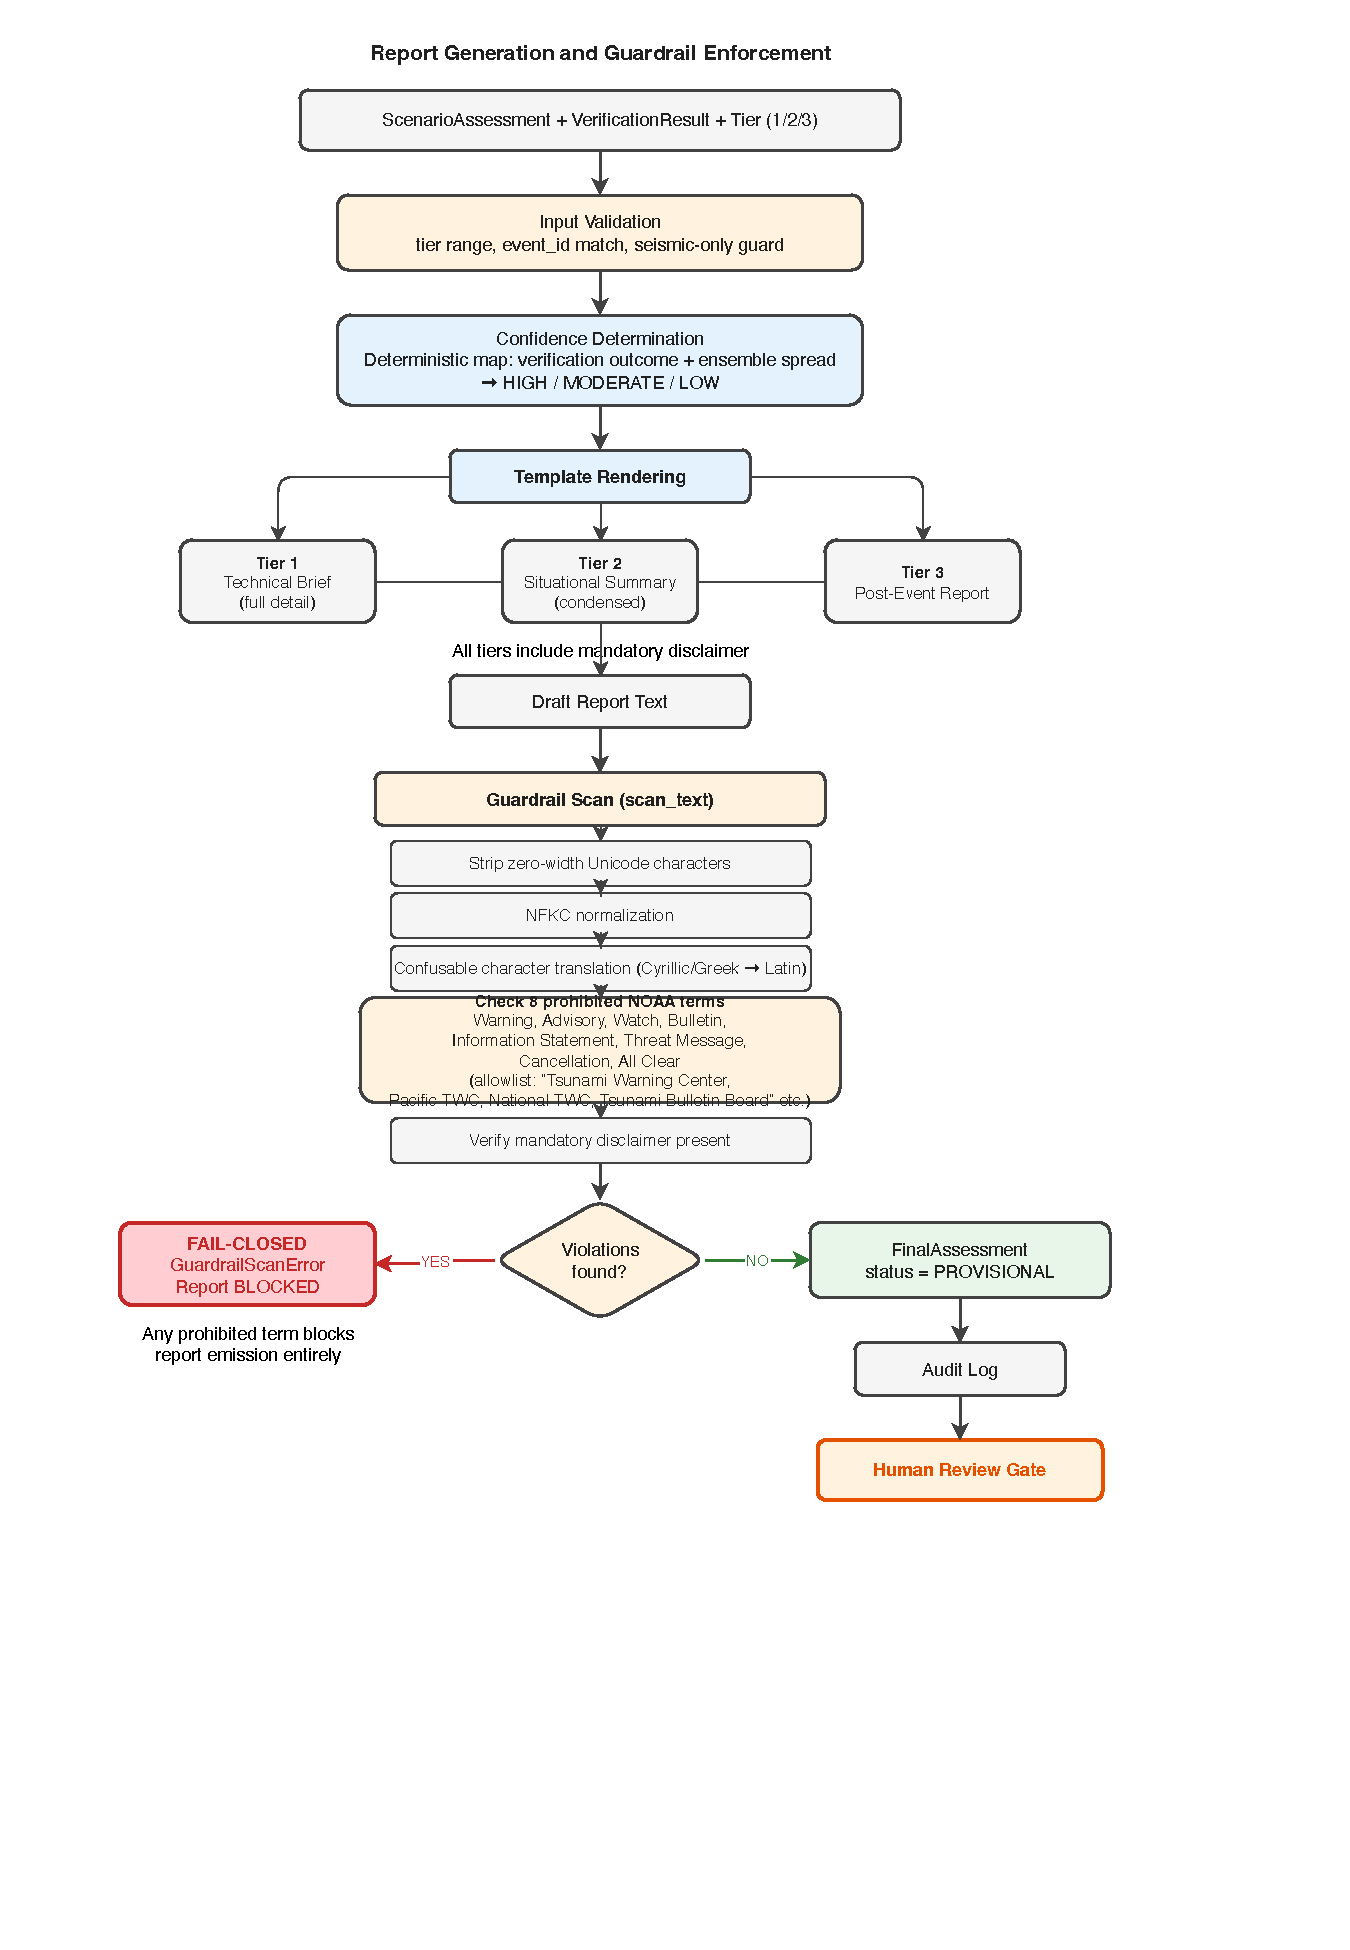
\includegraphics[width=\textwidth,height=0.85\textheight,keepaspectratio]{figures/report-guardrails-sequence.pdf}
\caption{Report generation and guardrail scanning sequence diagram.
  Template-based rendering (Tier 1/2/3) feeds into the guardrail
  scanner, which applies NFKC normalization, Unicode confusable
  detection, prohibited alert-term matching, and required disclaimer
  verification. Failed scans block report emission (fail-closed).}
\label{fig:uml-report-guardrails}
\end{figure}

\begin{figure}[ht!]
\centering
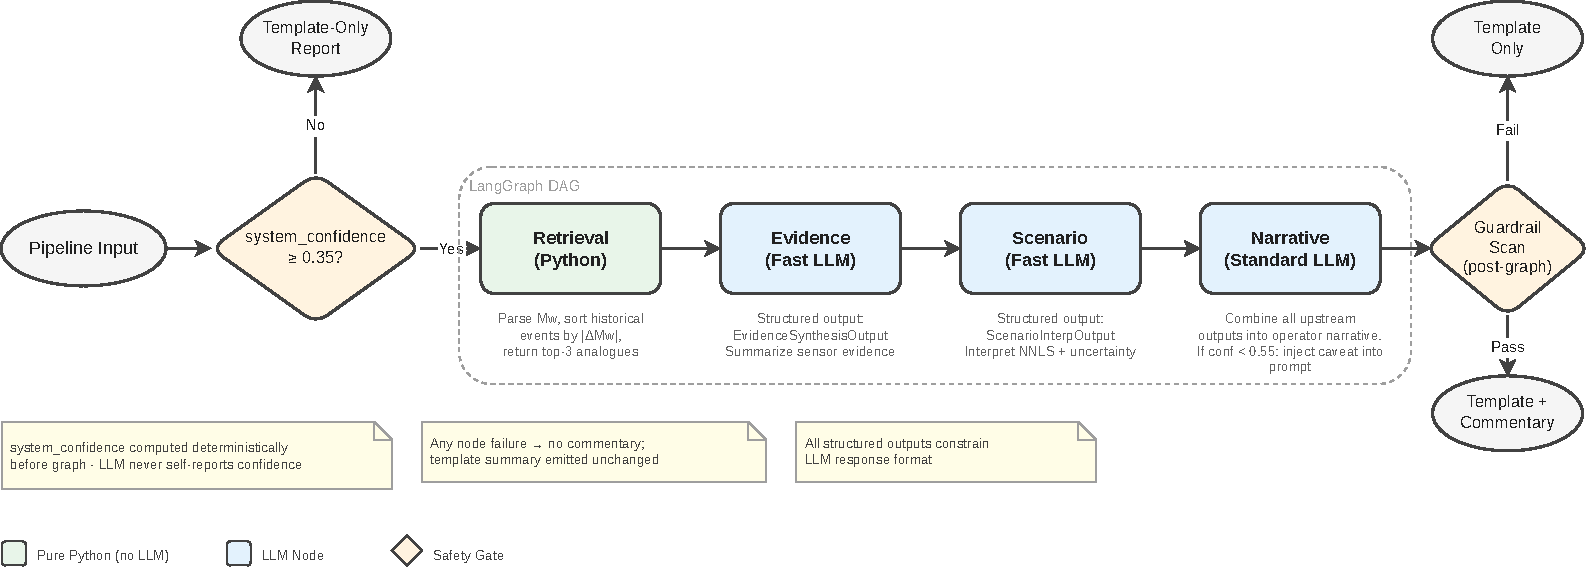
\includegraphics[width=\textwidth,height=0.85\textheight,keepaspectratio]{figures/llm-synthesis-graph.pdf}
\caption{LLM synthesis graph activity diagram. A 4-node linear
  LangGraph DAG (retrieval $\to$ evidence $\to$ scenario $\to$
  narrative) generates operator narratives in the Layer~3 advisory
  plane. The retrieval node is pure Python (magnitude-sorted historical
  analogue lookup); evidence and scenario nodes use a fast LLM with
  structured output; the narrative node uses a standard LLM. The graph
  is skipped entirely when system confidence $< 0.35$, and any node
  failure yields template-only output (no commentary) in
  \texttt{ReportAgent.synthesize()}.}
\label{fig:uml-llm-synthesis}
\end{figure}

\begin{figure}[ht!]
\centering
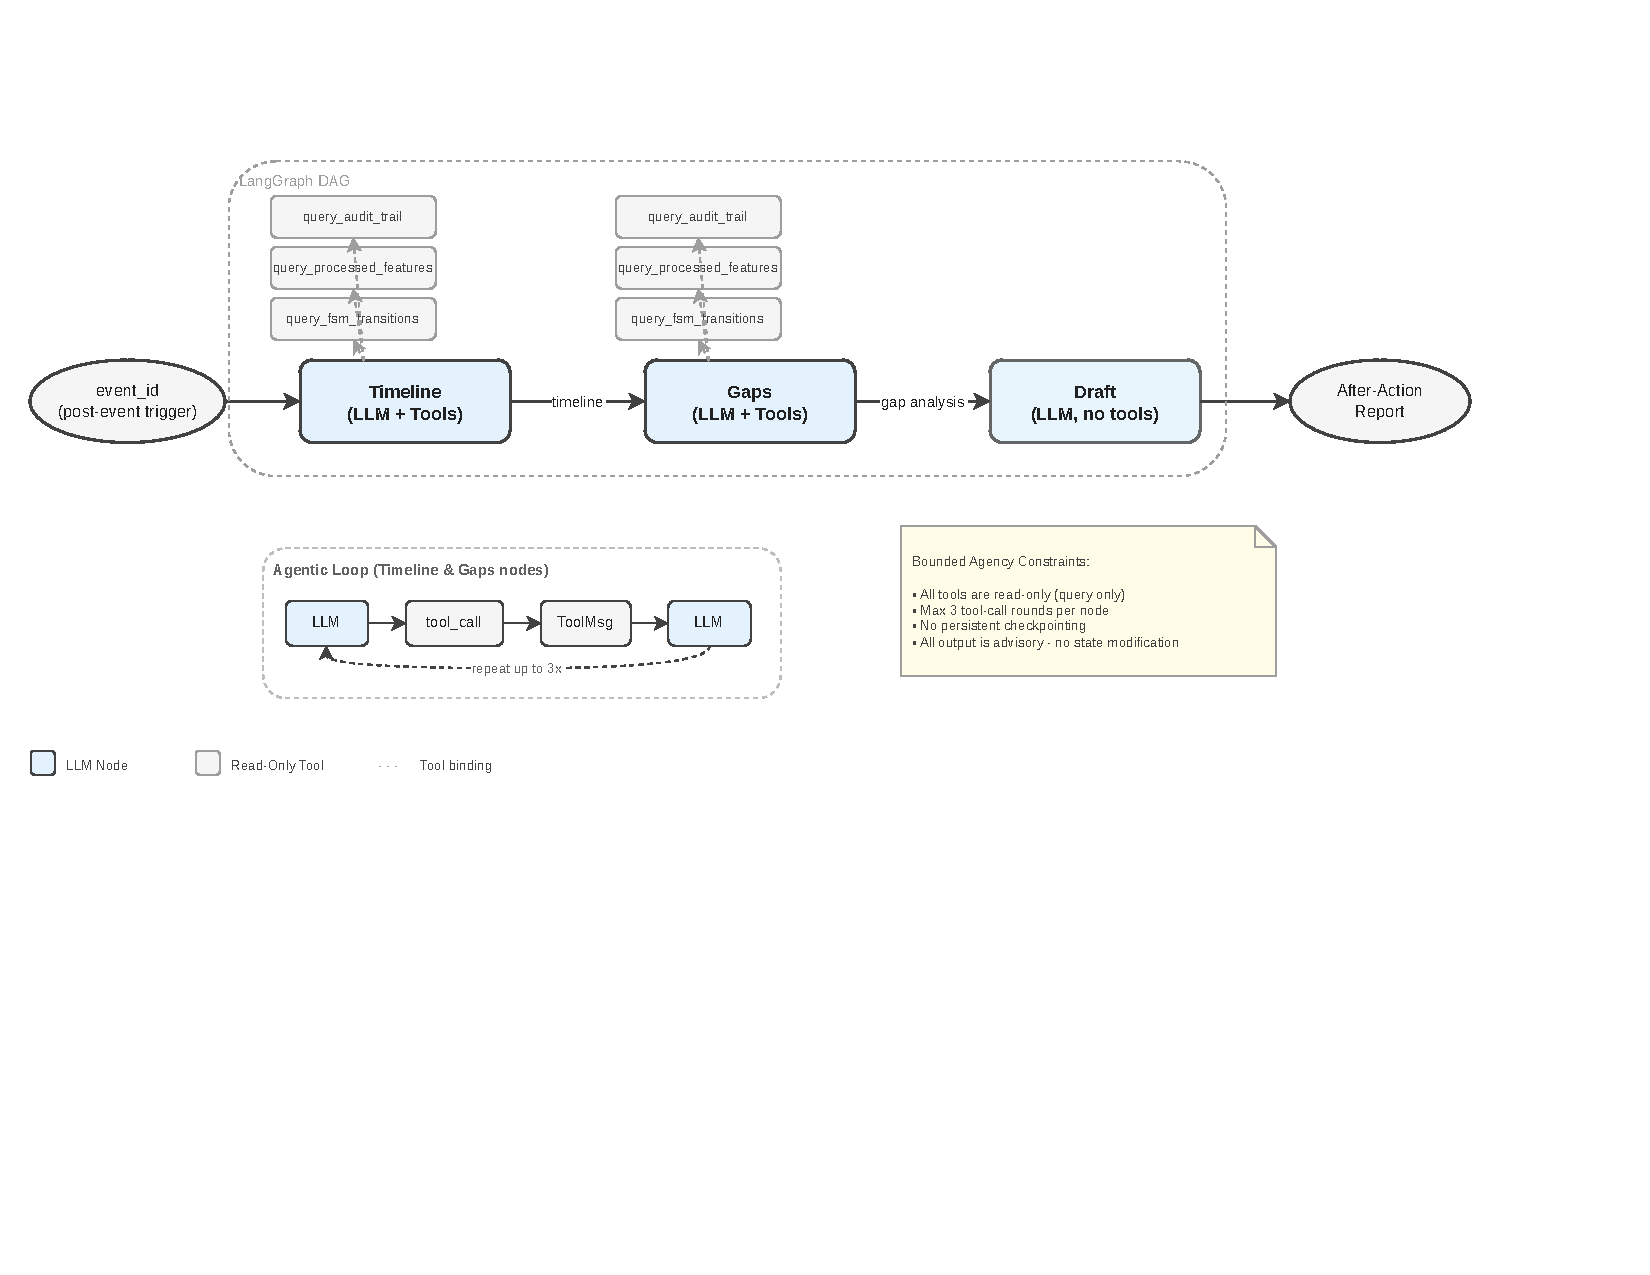
\includegraphics[width=\textwidth,height=0.85\textheight,keepaspectratio]{figures/after-action-graph.pdf}
\caption{After-action analysis graph with tool use. A 3-node LangGraph
  DAG (timeline $\to$ gaps $\to$ draft) performs post-event analysis.
  The timeline and gaps nodes use the agentic tool-use pattern: the LLM
  selects which read-only audit query tools to invoke (up to 3 rounds
  per node). The draft node synthesizes findings without tool access.
  All tools are bounded (read-only queries); the graph runs once
  per event with no persistent checkpointing.}
\label{fig:uml-after-action}
\end{figure}

\FloatBarrier
% ===================================================================
\section{Agent System Prompts}
\label{sec:appendix-prompts}
% ===================================================================

For reproducibility, we provide the full system prompts used in the LLM
advisory layer.  All prompts are versioned under source control
(\texttt{src/\allowbreak hazard\_assessment/\allowbreak agents/\allowbreak
llm\_advisory/\allowbreak prompts.py}).  The four processing agents
(QC, Anomaly, Scenario, Verification) and the FSM orchestrator contain
\emph{no} LLM prompts; they are purely deterministic.

\subsection{Real-Time Advisory Synthesis Graph}

The synthesis graph (Figure~\ref{fig:uml-llm-synthesis}) uses three
LLM-backed nodes.  The retrieval node is pure Python and has no prompt.
These prompts guide the LLM advisory layer that runs in parallel
with, but cannot override, the deterministic detection and
verification pipeline.

\promptlabel[promptfast]{Evidence Synthesis Prompt \normalfont\textnormal{\textit{(fast model)}}}
\begin{promptbox}
Summarize the sensor data in the <sensor_data> tags below for an on-duty
scientist who needs a quick read on the situation. Write 2-3 sentences.

Field definitions:
- Verification outcome: PASS (waveform matches scenario) or PASS_WITH_CONCERNS
  (matches, with recorded concerns).
- Active DART stations: number of DART BPR stations currently reporting data.
- Ensemble spread: LOW (well-constrained), MODERATE, or HIGH (ambiguous).
- Rayleigh wave suspect: true if the DART trigger may be seismic, not tsunami.
- System confidence: 0.0-1.0 composite score; below 0.55 means elevated
  uncertainty.

Rules:
- Describe what the instruments recorded, not what it implies for public safety.
- If rayleigh_wave_suspect is true, mention that the DART event-mode trigger
  may reflect seismic surface waves rather than a tsunami signal.
- Do NOT use the words "Warning", "Advisory", "Watch", "Information Statement",
  "Threat Message", "Cancellation", "All Clear", or "Bulletin". These are
  reserved for official NOAA products.
- Do NOT quote specific wave height numbers or arrival times.
- Do NOT include a self-assessed confidence statement.
\end{promptbox}

\promptlabel[promptfast]{Scenario Interpretation Prompt \normalfont\textnormal{\textit{(fast model)}}}
\begin{promptbox}
Interpret the NNLS scenario inversion results in the <scenario_data> tags
below. Write 2-3 sentences explaining the top-ranked scenario and what the
ensemble spread tells us.

Background: Each scenario is a weighted combination of pre-computed unit
sources (subfault segments from a unit-source propagation database). The NNLS
weights represent relative slip on each subfault; the equivalent moment
magnitude~\citep{hanks1979moment} is derived from the cumulative seismic
moment of the weighted sources.

Rules:
- Explain why the top scenario ranks first (e.g., best waveform fit).
- Note whether ensemble spread is LOW (well-constrained), MODERATE
  (some ambiguity), or HIGH (poorly constrained, multiple plausible sources).
- Do NOT predict specific coastal impacts or wave heights.
- Do NOT use "Warning", "Advisory", "Watch", "Information Statement",
  "Threat Message", "Cancellation", "All Clear", or "Bulletin". These are
  reserved for official NOAA products.
- Do NOT include a self-assessed confidence statement.
\end{promptbox}

The narrative synthesis prompt includes an \texttt{<historical\_context>}
XML block injected at runtime with JSON data from the historical analogue
lookup.  When \texttt{system\_confidence}~$< 0.55$, an elevated
uncertainty caveat is appended to the input.
The word limits (500 for Tier~1, 1000 for Tier~2) reflect the
different roles: Tier~1 supplements structured template tables with a
concise interpretive gloss, while Tier~2 is a standalone narrative
without supporting tables and must be self-contained.

\promptlabel[promptstandard]{Narrative Synthesis Prompt \normalfont\textnormal{\textit{(standard model)}}}
\begin{promptbox}
Write an internal operator brief that pulls together the evidence summary,
scenario interpretation, and any relevant historical context. The reader is
an on-duty seismologist or oceanographer.

<historical_context>
{similar_events_json}
</historical_context>

Structure:
1. Current evidence - what the sensors show.
2. Scenario interpretation - what the inversion suggests.
3. Historical context - comparable past events, if any are relevant.
4. Key uncertainties - what we do not yet know.

Rules:
- If system_confidence < 0.55, include a sentence flagging elevated uncertainty.
- Historical events are background context, not predictions. Do NOT cite past
  wave heights as forecasts for the current event.
- Do NOT use "Warning", "Advisory", "Watch", "Information Statement",
  "Threat Message", "Cancellation", "All Clear", or "Bulletin".
- Do NOT state specific numerical predictions for wave heights or arrival times.
- Keep the narrative under 500 words for Tier 1, under 1000 for Tier 2.
\end{promptbox}

\subsection{Post-Event After-Action Analysis Graph}

The after-action graph (Figure~\ref{fig:uml-after-action}) runs
post-event using a quality-tier model.  The timeline and gaps nodes use
LLM-directed tool calls (up to 3~rounds each) against read-only audit
query tools.
The API refuses analysis of the event the FSM currently holds and of
events with no audit history, so the graph is used after an event
rather than during it. The system has no trusted event-disposition
record, so this gate does not establish that an event is closed. Every tool call the model makes is recorded,
tool results carry explicit truncation flags, and the resulting report
is persisted to the audit trail.

\promptlabel[promptquality]{Timeline Reconstruction Prompt \normalfont\textnormal{\textit{(quality model, tool use)}}}
\begin{promptbox}
Reconstruct a chronological timeline of the event using the provided tools.
Query the audit trail and FSM transition log to answer: what happened, when,
and in what order?

For each entry, note:
- What occurred (FSM transition, agent output, human decision)
- The timestamp
- Anything unusual, such as delays, skipped steps, or repeated transitions

Use query_audit_trail and query_fsm_transitions to pull the data.
Focus on the critical path from initial detection through escalation to the
human decision. Keep the timeline to 200-400 words.
\end{promptbox}

\promptlabel[promptquality]{Detection Gap Analysis Prompt \normalfont\textnormal{\textit{(quality model, tool use)}}}
\begin{promptbox}
Review the timeline above and use the provided tools to find detection gaps
and bottlenecks. Look for:
1. Detection delays: how long between the earthquake and first threshold
   crossing?
2. Data gaps: stations that went silent, QC failures, missing windows.
3. Near-misses: scores that came close to a threshold but did not cross it.
4. Process bottlenecks: slow state transitions or delayed human review.

Use query_audit_trail and query_processed_features as needed.
Cite specific timestamps, station IDs, and threshold values.
Keep the analysis to 200-500 words.
\end{promptbox}

\promptlabel[promptquality]{Incident Report Draft Prompt \normalfont\textnormal{\textit{(quality model, no tools)}}}
\begin{promptbox}
Using the timeline and gap analysis above, draft a structured after-action
report with these sections:

1. Event Summary (2-3 sentences)
2. Timeline of Key Events (chronological list)
3. Detection Performance (what worked, what fell short)
4. Gaps and Recommendations
5. Lessons Learned

Write for colleagues who will read this in a post-event debrief. Be direct
and specific. Quote numbers, not generalities.
Keep the report to 500-1000 words.
\end{promptbox}

\FloatBarrier
% ===================================================================
\section{FSM Orchestrator Transition Rules}
\label{sec:appendix-fsm}
% ===================================================================

The FSM orchestrator is entirely deterministic: no LLM is in the
decision path.  Table~\ref{tab:fsm-rules} summarizes all valid
transitions and their trigger conditions.

\begin{center}
\begin{minipage}{\linewidth}
\centering
\captionof{table}{FSM state transition rules.  Default thresholds:
  $T_1 = 0.35$, $T_2 = 0.60$, $T_3 = 0.85$, $M_{\mathrm{esc}} = 7.5$,
  monitor timeout = 12\,h.  $s$ denotes the current ensemble anomaly score.}
\label{tab:fsm-rules}
\small
\begin{tabular}{@{}llp{5.5cm}@{}}
\toprule
From & To & Trigger condition \\
\midrule
IDLE & MONITOR & Seismic event with $M \geq 6.0$ in tsunamigenic zone \\
\addlinespace
MONITOR & INVESTIGATE & $s \geq T_1$; or $M \geq M_{\mathrm{esc}}$ with DART event-mode activation (seismic override prevents holding in MONITOR on a sub-$T_1$ score) \\
MONITOR & ESCALATE & $M \geq M_{\mathrm{esc}}$ AND depth $< 100$\,km (seismic-only; fires as chained IDLE$\to$MONITOR$\to$ESCALATE) \\
MONITOR & IDLE & Timeout: $\geq 12$\,h elapsed and $s < T_1$ \\
\addlinespace
INVESTIGATE & ASSESS & $s \geq T_2$ \\
INVESTIGATE & MONITOR & $s < T_1$ (de-escalation; suppressed when $M \geq 7.5$ with DART event-mode$\to$ASSESS) \\
\addlinespace
ASSESS & ESCALATE & $s \geq T_3$ \\
ASSESS & ESCALATE & $M \geq M_{\mathrm{esc}}$ with DART event-mode activation (seismic override) \\
ASSESS & INVESTIGATE & $s < T_2$ (de-escalation) \\
\addlinespace
ESCALATE & IDLE & Explicit event resolution (\texttt{resolve\_event()}; no API route invokes it. APPROVE, REJECT and DEFER are all recorded without changing FSM state) \\
\bottomrule
\end{tabular}
\end{minipage}
\end{center}

The seismic override ($M \geq 7.5$ with DART event-mode activation)
acts in every score-driven state: it advances MONITOR to INVESTIGATE,
suppresses de-escalation from INVESTIGATE (advancing to ASSESS), and
bypasses the $T_3$ anomaly threshold from ASSESS.  This ensures
that large earthquakes with DART event-mode activation reach human
review even when the ensemble score has not converged above the
thresholds.  ESCALATE
$\to$ IDLE requires human resolution; automated de-escalation from
ESCALATE is intentionally forbidden.

% ============================================================
%  Appendix D: Multi-Source Data Availability
% ============================================================

\newpage
\renewcommand{\thefigure}{D.\arabic{figure}}
\setcounter{figure}{0}
\section{Multi-Source Data Availability}
\label{sec:appendix-coops}

Figure~\ref{fig:multi-source-network} shows the full operational
observation network: all 43~DART bottom pressure recorders listed on
NDBC as of March 2026, spanning the Pacific, Atlantic, Caribbean, Gulf
of Mexico, and Indian Ocean basins, together with all 301~active CO-OPS
tide gauge stations along U.S.\ coastlines, Pacific islands, Alaska,
the Caribbean, and the Great Lakes.  The subsequent figures present CO-OPS water-level
observations retrieved from the NOAA CO-OPS API during all five evaluation
events, demonstrating the availability of complementary
water-level data streams referenced in Section~\ref{sec:architecture}.
The CO-OPS anomaly detection pipeline is implemented and wired; real-event
retrospective validation with these data streams remains future work
(see Limitation~11 in Section~\ref{sec:discussion}).

\begin{figure}[ht!]
\centering
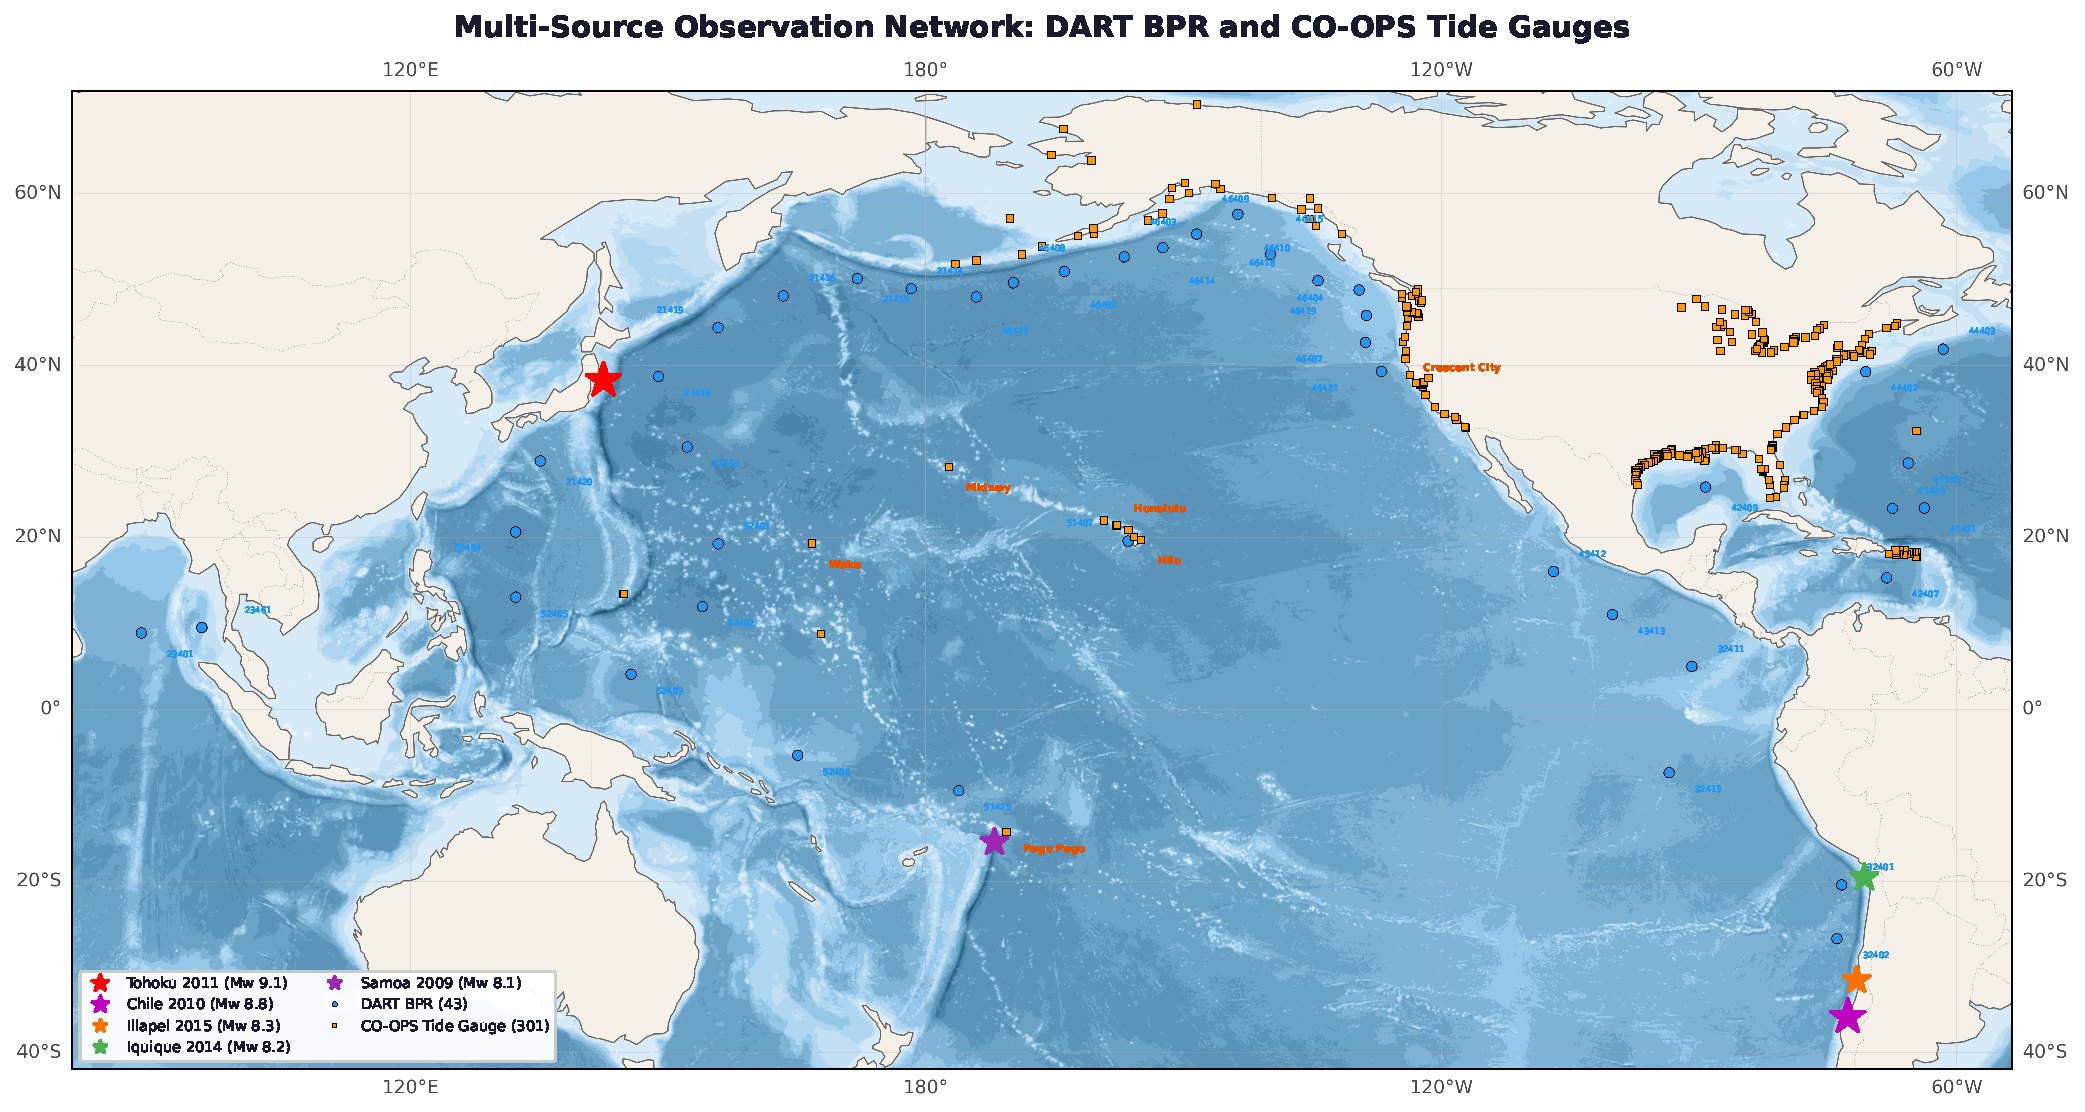
\includegraphics[width=0.95\linewidth]{figures/fig_multi_source_network.pdf}
\caption{Multi-source observation network spanning the global ocean basins.
  Stars mark the five evaluation epicenters: Tohoku 2011, Chile 2010,
  Illapel 2015, Iquique 2014, and Samoa 2009.
  Blue circles: all 43 operational DART bottom pressure recorders (NDBC, March 2026).
  Orange squares: all 301 active CO-OPS tide gauge stations (NOAA API,
  March 2026); named labels highlight the six stations with water-level
  data shown in Figures~\ref{fig:coops-tohoku}--\ref{fig:coops-samoa}.
  The USGS seismic event feed (not shown) provides the initial
  earthquake trigger that activates the FSM; DART polling switches to
  the faster event-mode interval per station once event-mode data rows
  are observed.}
\label{fig:multi-source-network}
\end{figure}

\begin{figure}[ht!]
\centering
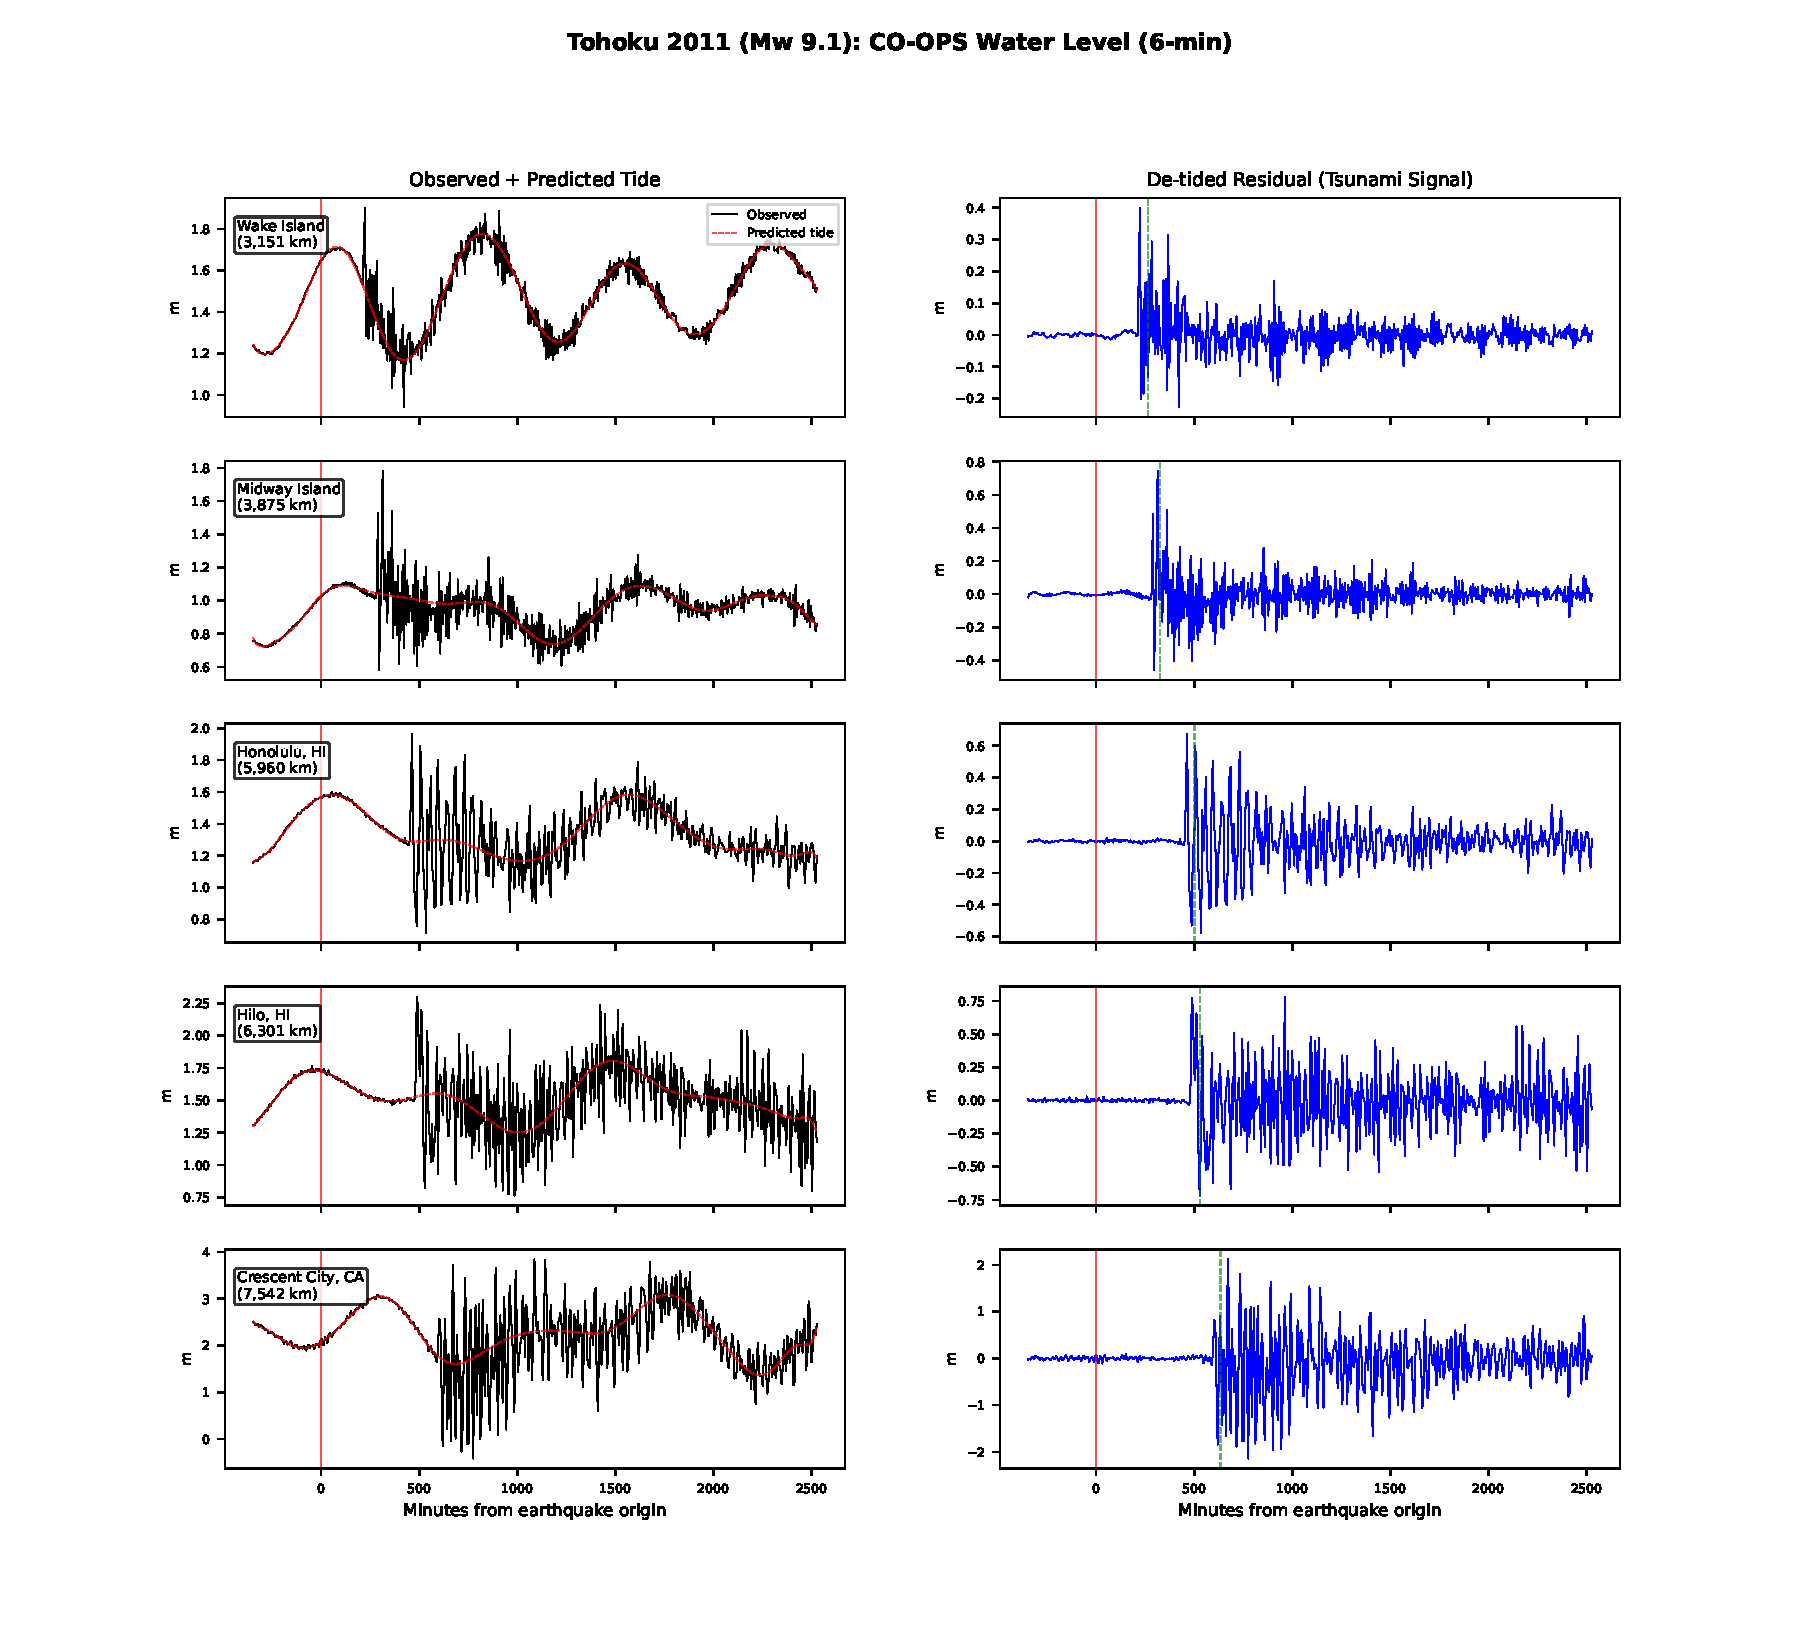
\includegraphics[width=0.95\linewidth]{figures/fig_coops_tohoku.pdf}
\caption{CO-OPS 6-minute water-level records at five Pacific tide gauge
  stations during Tohoku 2011, including Crescent City, CA, a site with
  known 3--4$\times$ tsunami amplification due to harbor geometry.
  Left: observed water level (black) with IRLS 8-constituent harmonic
  tidal fit (red dashed).  Right: de-tided residual;
  green dashed line marks estimated tsunami arrival
  ($d/c$, $c{=}198$\,m/s).
  Stations ordered by epicentral distance.}
\label{fig:coops-tohoku}
\end{figure}

\begin{figure}[ht!]
\centering
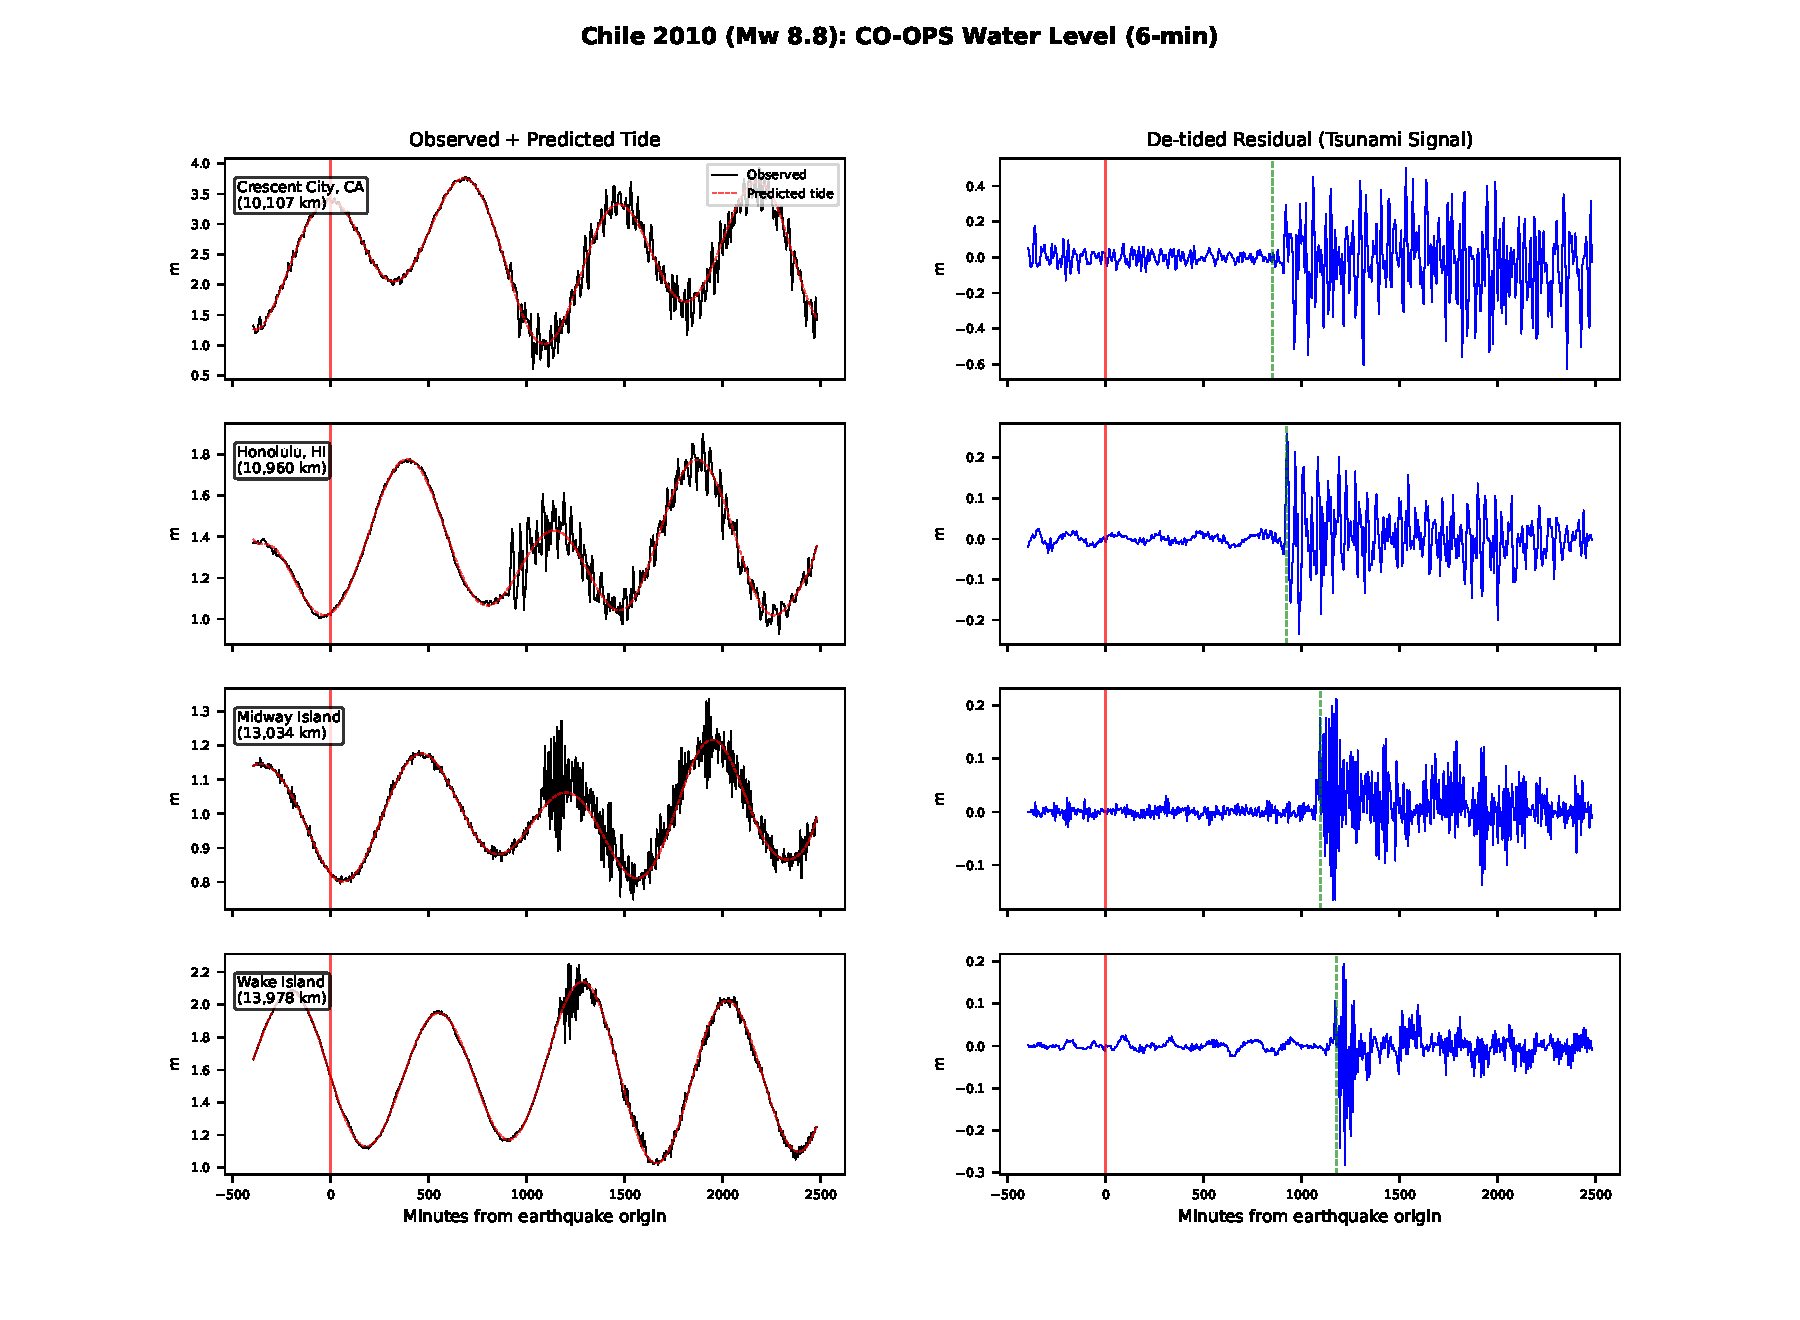
\includegraphics[width=0.95\linewidth]{figures/fig_coops_chile.pdf}
\caption{CO-OPS 6-minute water-level records at four Pacific tide gauge
  stations during Chile 2010, including Crescent City, CA (top).
  Left: observed (black) with IRLS tidal fit (red dashed).
  Right: de-tided residual; green dashed line marks estimated tsunami arrival.
  Note: Hilo observations unavailable (gauge outage Feb.\ 24 to Mar.\ 1, 2010).}
\label{fig:coops-chile}
\end{figure}

\begin{figure}[ht!]
\centering
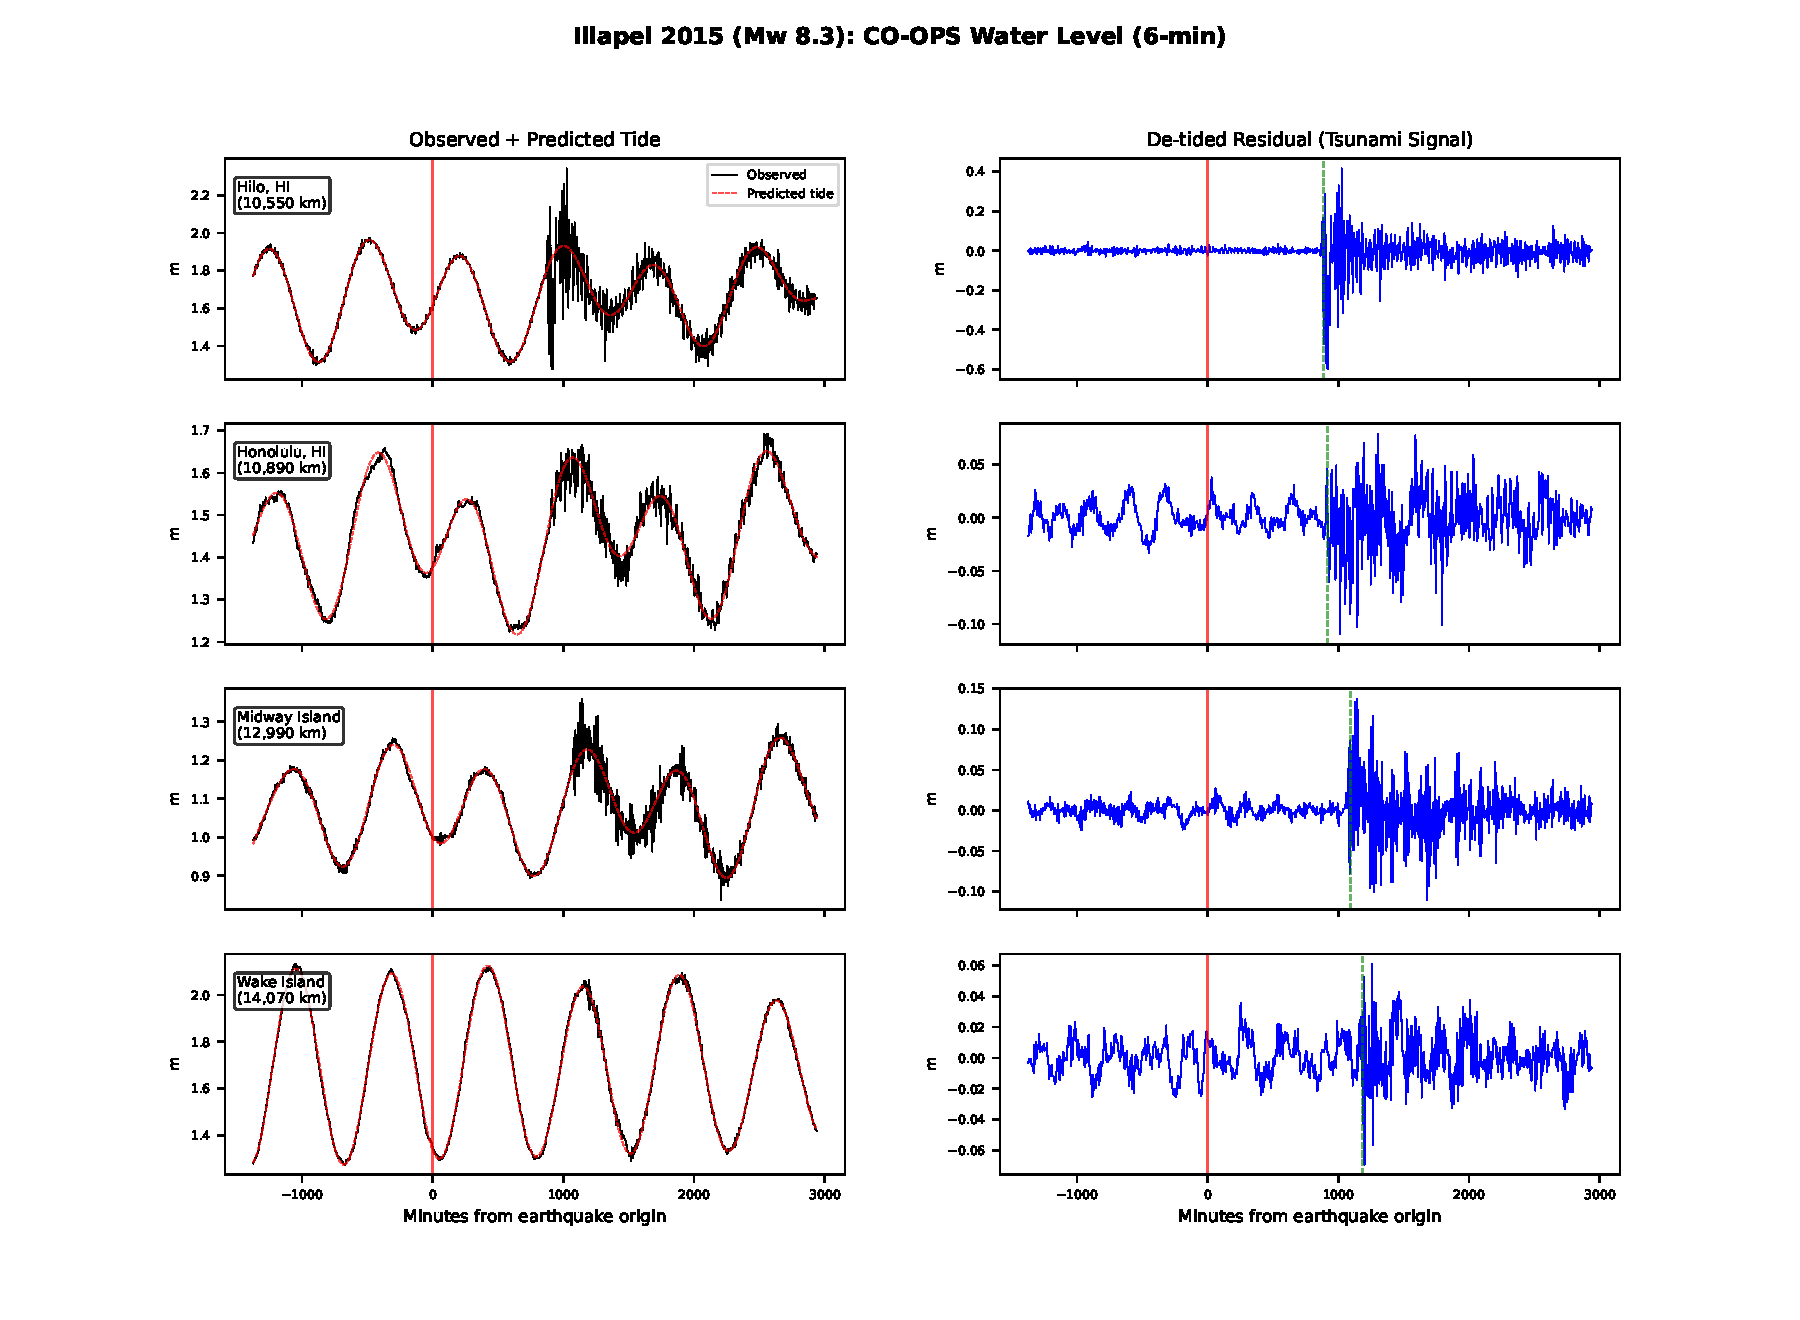
\includegraphics[width=0.95\linewidth]{figures/fig_coops_illapel.pdf}
\caption{CO-OPS 6-minute water-level records at four Pacific tide gauge
  stations during Illapel 2015.
  Left: observed (black) with IRLS tidal fit (red dashed).
  Right: de-tided residual; green dashed line marks estimated tsunami arrival.
  Stations ordered by epicentral distance.}
\label{fig:coops-illapel}
\end{figure}

\begin{figure}[ht!]
\centering
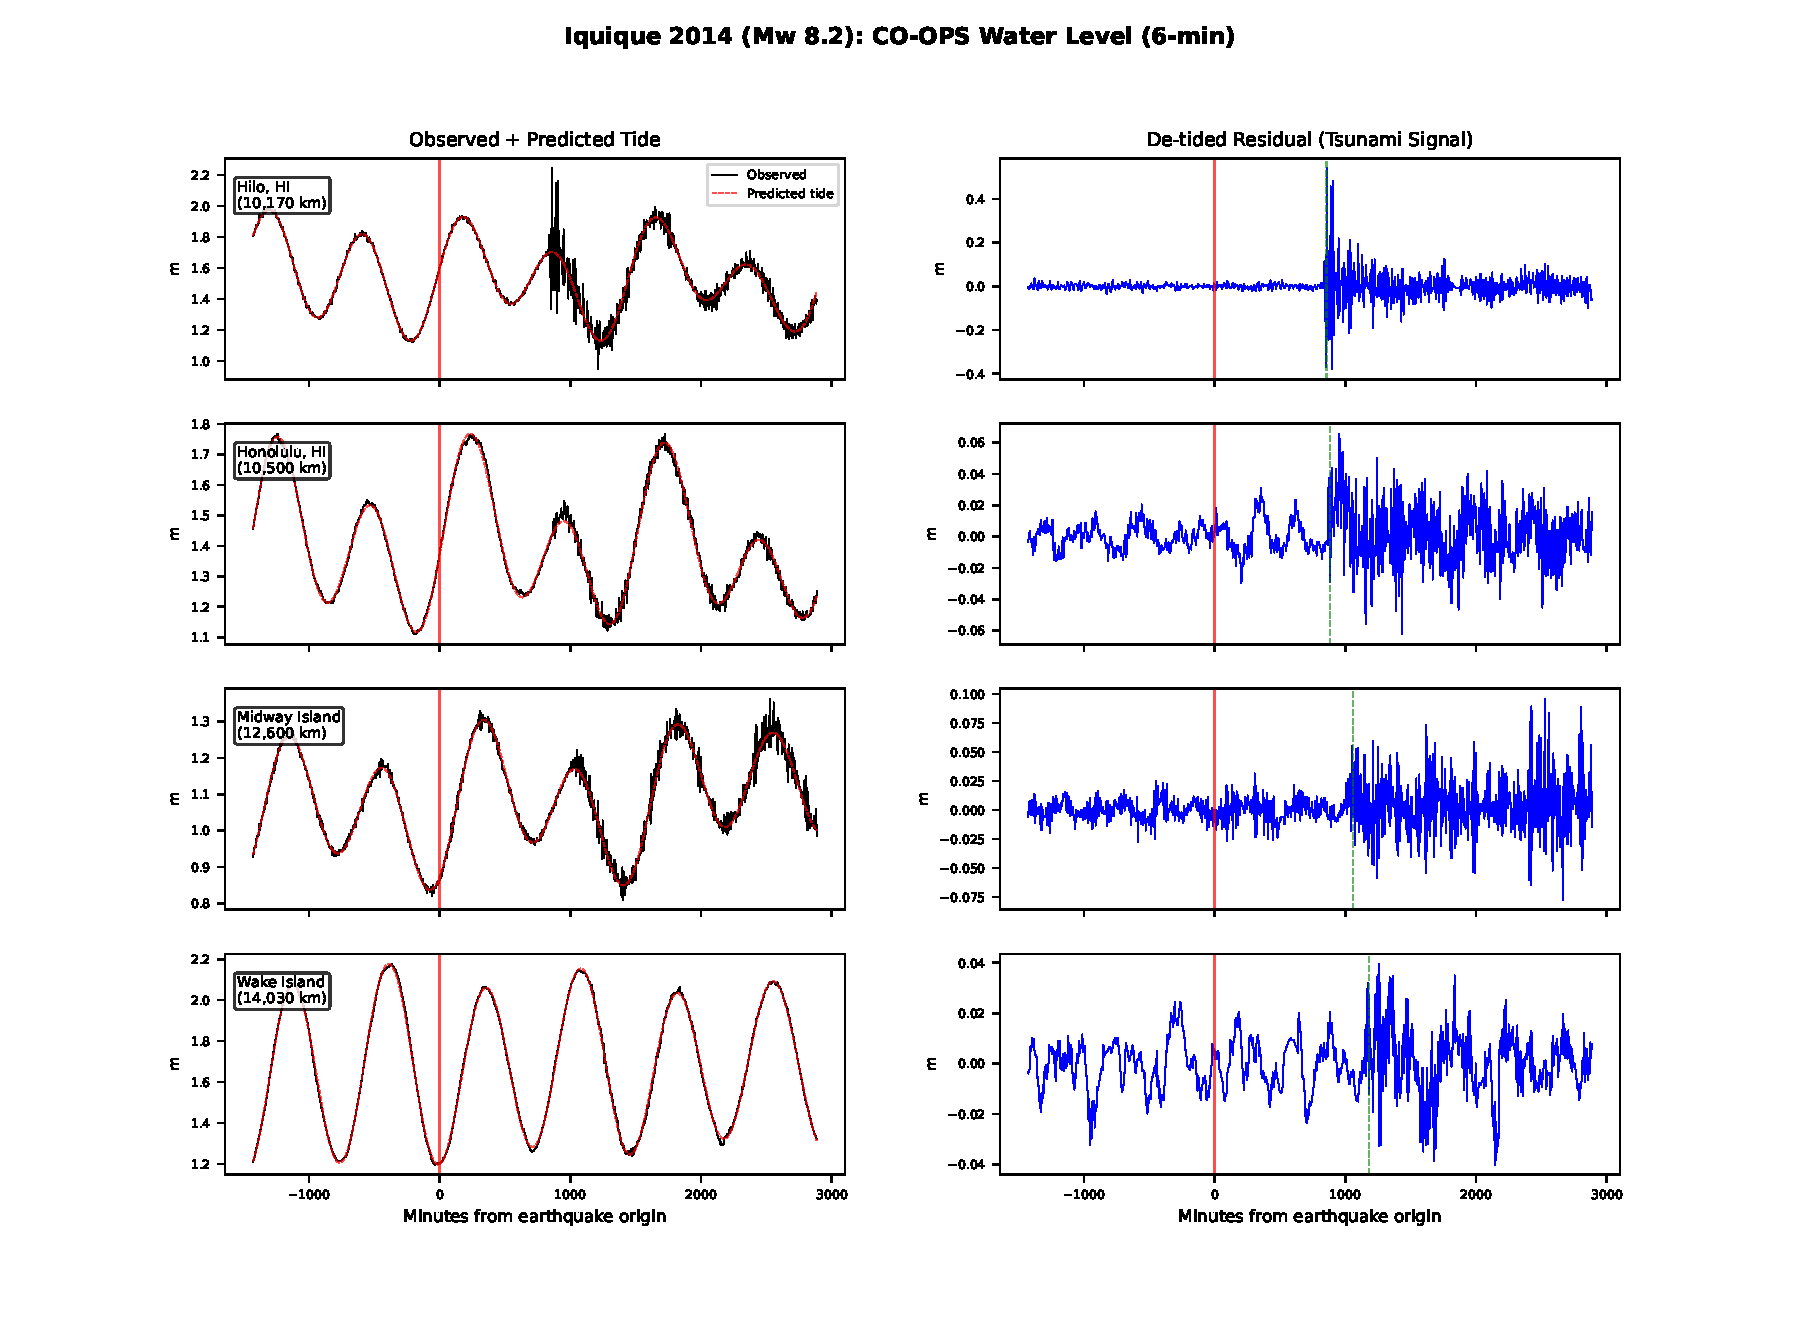
\includegraphics[width=0.95\linewidth]{figures/fig_coops_iquique.pdf}
\caption{CO-OPS 6-minute water-level records at four Pacific tide gauge
  stations during Iquique 2014.
  Left: observed (black) with IRLS tidal fit (red dashed).
  Right: de-tided residual; green dashed line marks estimated tsunami arrival.
  Stations ordered by epicentral distance.}
\label{fig:coops-iquique}
\end{figure}

\begin{figure}[ht!]
\centering
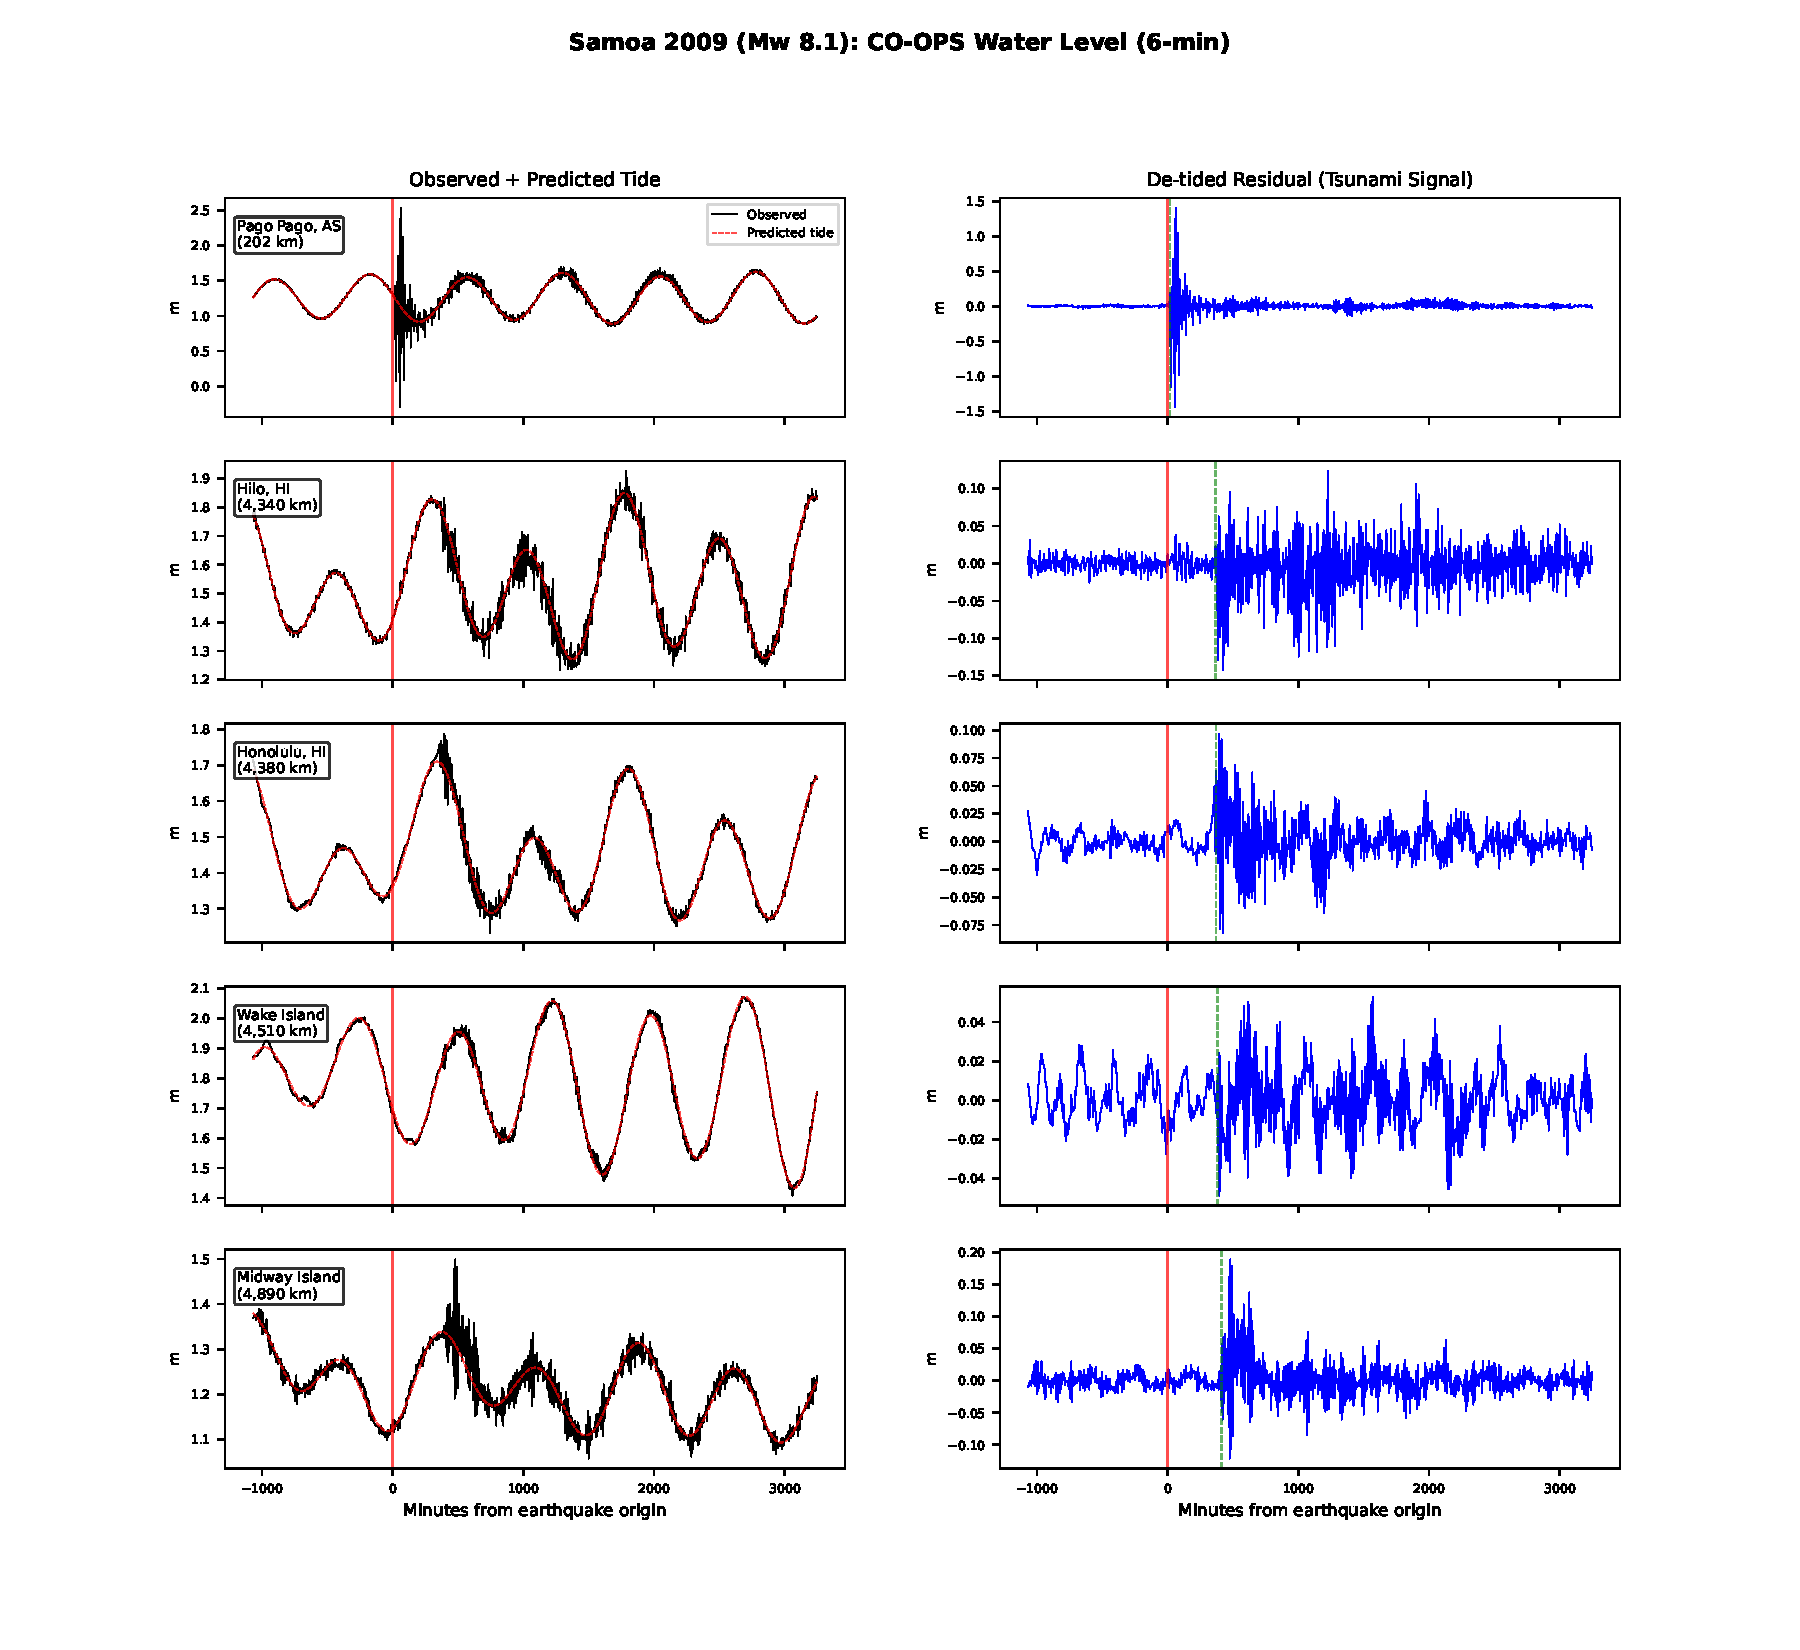
\includegraphics[width=0.95\linewidth]{figures/fig_coops_samoa.pdf}
\caption{CO-OPS 6-minute water-level records at five Pacific tide gauge
  stations during Samoa 2009, including Pago Pago, American Samoa
  (top; 202\,km from epicenter), the only near-field coastal station.
  Left: observed (black) with IRLS tidal fit (red dashed).
  Right: de-tided residual; green dashed line marks estimated tsunami arrival.
  Stations ordered by epicentral distance.}
\label{fig:coops-samoa}
\end{figure}

% ============================================================
%  Appendix E: Mission Control Dashboard
% ============================================================

\newpage
\renewcommand{\thefigure}{E.\arabic{figure}}
\setcounter{figure}{0}
\section{Mission Control Dashboard}
\label{sec:appendix-dashboard}

The Mission Control dashboard provides real-time operational
awareness through a browser-based React interface.  The layout
(Figure~\ref{fig:dashboard-layout}) follows a three-column CSS Grid:
a narrow left column, a wide center column occupied by the map, and a
right column for review and events, with full-width header and audit
strips.

\begin{itemize}[nosep]
  \item \textbf{Header bar} (full width): connection and
    non-authoritative-use notices, summary readouts (active event,
    event-mode DART count, first $T_1$ crossing where available, and
    latest anomaly score), the age of the last successful core-API poll,
    a UTC clock, and the current FSM state as a large color-coded readout.
  \item \textbf{Left column}: FSM Orchestrator (five-state ladder with
    transition history and dwell times) above Component Registry (per
    component: name, role, and execution path, that is, live worker or
    offline evaluation only).
  \item \textbf{Center}: Ocean Map (Leaflet-based Pacific view with
    DART and CO-OPS station markers, a legend, labels on triggered
    stations, epicenter annotation, and a 500\,km distance circle),
    spanning both content rows; an Anomaly Score Timeline (Recharts
    area chart holding the most recent 60 samples, appended on each
    score change plus a 30\,s keepalive, with $T_1$/$T_2$/$T_3$
    reference lines) is embedded along the map's lower edge.
  \item \textbf{Right column}: Human Review Gate
    (APPROVE/REJECT/DEFER controls, active only during ESCALATE, with
    an evidence-acknowledgment step; the controls stay pinned below the
    scrolling evidence so they remain reachable) above Active Event
    (current event details and station coverage).
  \item \textbf{Activity strip} (full width, bottom): append-only audit
    entries streamed via WebSocket. Consecutive entries of the same type
    from the same producer collapse into one row carrying a count, because
    the worker writes one anomaly-scoring entry per scored window and an
    uncollapsed strip showed nothing else.
\end{itemize}

All data flow through a single WebSocket connection
(\texttt{/api/mc/ws/live}) that streams FSM snapshots, agent
statuses, and recent audit entries. Snapshots are sent only when they
change, so the connection also carries a throttled heartbeat reporting the
last successful core-API poll; without it a console watching an uneventful
basin would be indistinguishable from one whose upstream had failed.
Recorded review decisions are queried separately rather than read out of
the general audit window, which per-window anomaly entries can fill within
a fraction of a second.  The dashboard has no write
capability to the pipeline; only the Human Review Gate issues
decisions through a separate service-authenticated REST endpoint
(reviewer identity is caller-asserted and recorded as such).
During a developing event, the duty scientist monitors the anomaly
score timeline and FSM state transitions in real time.  When the FSM
reaches \textsc{escalate}, the Human Review Gate activates, presenting
the generated assessment for APPROVE, REJECT, or DEFER based on the
evidence chain visible in the audit log.

\FloatBarrier
\begin{figure}[!htbp]
\centering
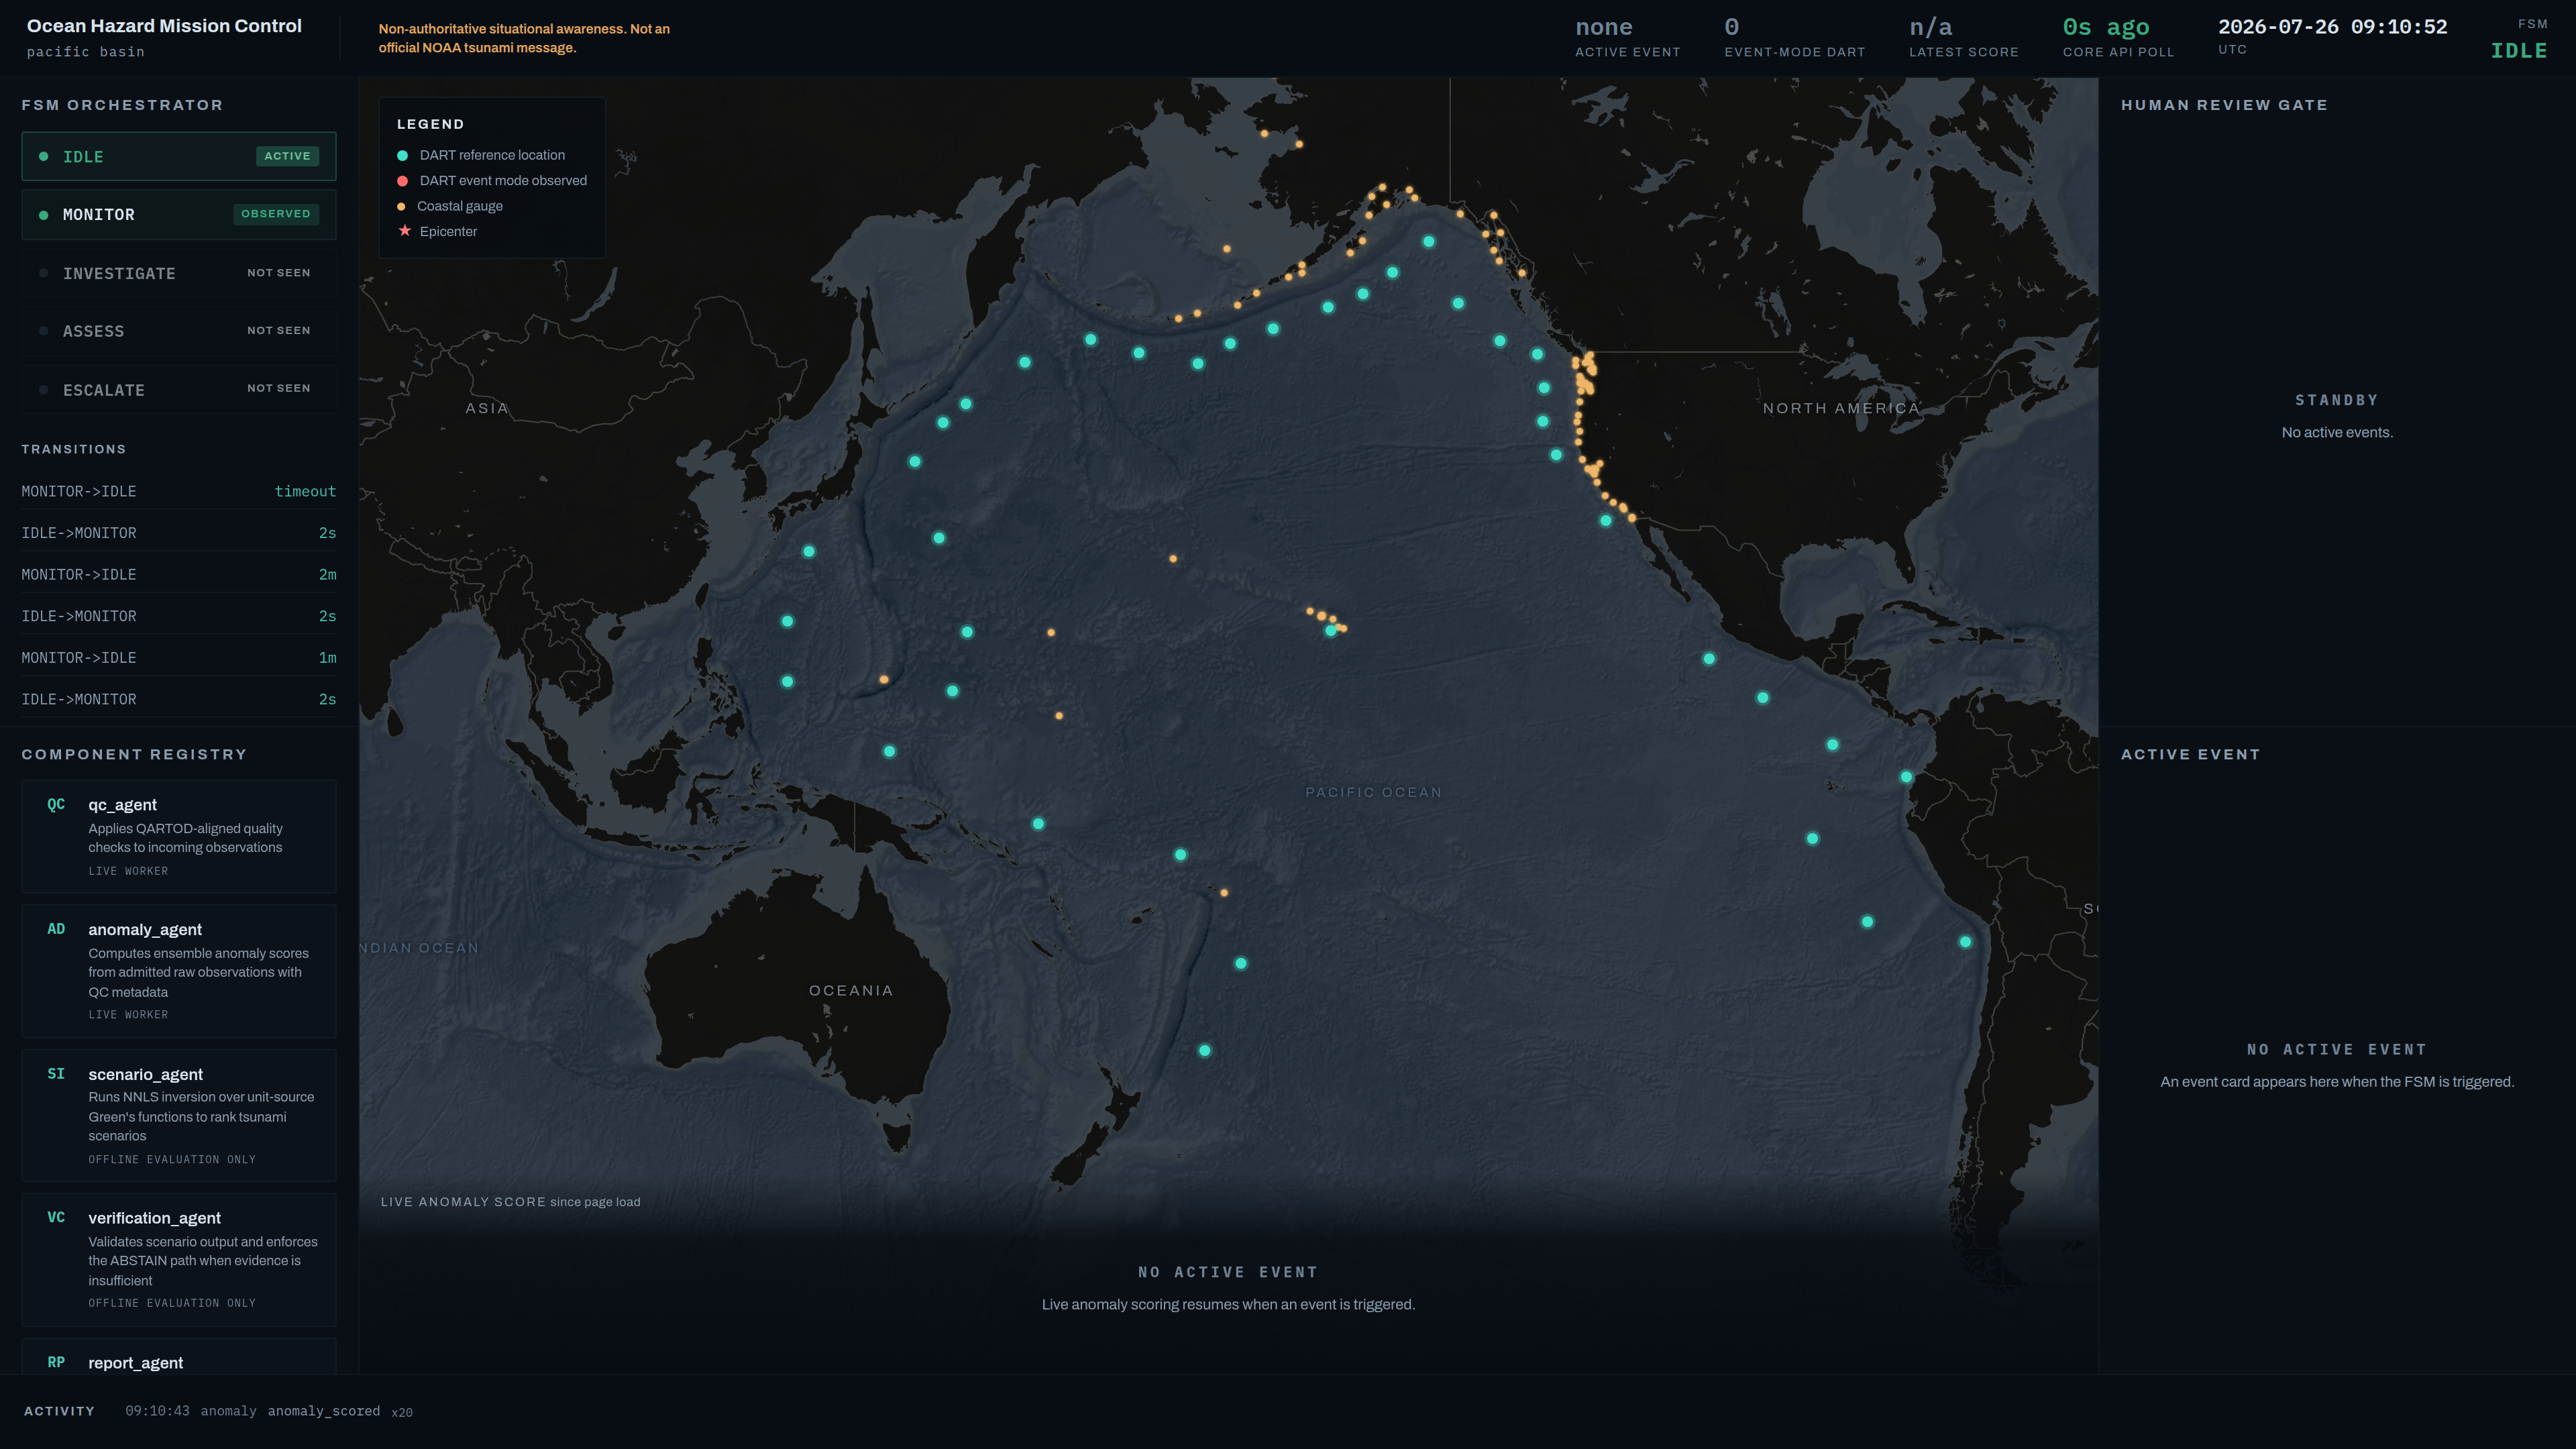
\includegraphics[width=0.95\linewidth]{figures/fig_dashboard_layout_updated.png}
\caption{Mission Control dashboard screenshot showing the system in
  \textsc{idle} state.  The three-column asymmetric grid places the
  FSM state panel (left) and Human Review Gate (right) flanking the
  central Pacific Ocean DART station map and anomaly score timeline.
  The header bar displays real-time UTC clock, FSM state, and
  ensemble anomaly score.  The Human Review Gate (top right) is the
  only interactive control surface; all other panels are read-only
  displays of pipeline state streamed via WebSocket from a live
  backend at capture time.}
\label{fig:dashboard-layout}
\end{figure}

% ============================================================
%  Appendix F: Agent Interaction Trace Example
% ============================================================

\newpage
\renewcommand{\thefigure}{F.\arabic{figure}}
\setcounter{figure}{0}
\section{Agent Interaction Trace Example}
\label{sec:appendix-trace}

Each pipeline stage produces a typed Pydantic envelope that serves
as the input to the next agent and is recorded in the audit trail.
The traces below were generated by
\texttt{scripts/run\_synthetic\_pipeline.py} on synthetic data
(M8.5 Aleutian and M7.0 moderate scenarios).
The QC, AnomalyAssessment, and FSM envelopes are produced by
actual pipeline execution.  The ScenarioAssessment and
VerificationResult envelopes are illustrative examples of the
expected output schema, as the scenario inversion and verification
agents require real DART waveform data that is not available for
synthetic events.

% Auto-generated by scripts/run_synthetic_pipeline.py
% Styled with agent-specific trace boxes; annotations are filled from
% the live trace values. Edit the templates in the script, not here.

\subsection*{Trace 1: M8.5 Aleutian}

\noindent The M8.5 Aleutian scenario exercises the full escalation path.
The shallow M8.5 earthquake meets the seismic-only criteria, so the
FSM escalates immediately as a chained
IDLE~$\to$~MONITOR~$\to$~ESCALATE transition
(Algorithm~\ref{alg:fsm}, lines~3--5) without waiting for ocean
data.  The ensemble anomaly score (0.55) subsequently exceeds
$T_1 = 0.35$, corroborating the seismic trigger with ocean-based
evidence: the threshold component dominates (0.74), while the
statistical component contributes a moderate 0.28.

\medskip
\noindent\textit{QC Agent validates incoming records and reports per-station
usability, confidence, evaluated-check coverage, and data mode:}

\tracelabel[traceqc]{QC Agent Output}
\begin{tracebox}
{
  "n_records": 20,
  "sample_report": {
    "station_id": "21413",
    "record_usable": true,
    "station_confidence": 1.0,
    "n_checks_evaluated": 0,
    "data_mode": "EVENT"
  }
}
\end{tracebox}

\noindent\textit{Anomaly Agent fuses threshold, wavelet, and BOCPD
detectors into a single ensemble score and identifies triggering
stations:}

\tracelabel[traceanomaly]{Anomaly Assessment}
\begin{tracebox}
{
  "type": "AnomalyAssessment",
  "schema_version": "1.0",
  "producer": "anomaly_agent",
  "anomaly_score": 0.5514,
  "score_components": {
    "threshold": 0.7425,
    "statistical": 0.2784,
    "ml": null
  },
  "triggering_stations": [
    "21413"
  ],
  "scored_stations": [
    "21413"
  ],
  "seismic_quiet": true,
  "filter_degraded": false
}
\end{tracebox}

\noindent\textit{FSM Orchestrator records each deterministic state
transition with its trigger condition:}

\tracelabel[tracefsm]{FSM Orchestrator}
\begin{tracebox}
{
  "after_seismic_trigger": "ESCALATE",
  "after_anomaly_score": "ESCALATE",
  "magnitude": 8.5,
  "anomaly_score": 0.5514,
  "transitions": [
    {
      "from": "IDLE",
      "to": "MONITOR",
      "trigger": "seismic"
    },
    {
      "from": "MONITOR",
      "to": "ESCALATE",
      "trigger": "seismic"
    }
  ]
}
\end{tracebox}

\noindent\textit{Scenario and Verification envelopes illustrate the expected
output schema (the inversion and verification agents need real
DART waveforms, which synthetic events do not provide):}

\tracelabel[tracescenario]{Scenario Assessment (illustrative)}
\begin{tracebox}
{
  "method": "NNLS_UNIT_SOURCE",
  "constraint_stage": "DART_CONSTRAINED",
  "dart_stations_used": [
    "21413"
  ],
  "top_scenarios": [
    {
      "unit_source_ids": [
        "src_aleutian_01"
      ],
      "weights": [
        1.0
      ],
      "waveform_rmse_cm": 1.2,
      "mw_equivalent": 8.5,
      "rank": 1,
      "posterior_weight": 0.85
    }
  ],
  "ensemble_spread": "LOW"
}
\end{tracebox}

\tracelabel[traceverify]{Verification Result (illustrative)}
\begin{tracebox}
{
  "overall": "PASS",
  "checks": [
    {
      "name": "holdout_station_validation",
      "result": "PASS",
      "evidence": "Holdout RMSE 1.2 cm < 3.0 cm threshold"
    },
    {
      "name": "data_coverage",
      "result": "PASS",
      "evidence": "1/1 DART stations used (100%)"
    },
    {
      "name": "physical_consistency",
      "result": "PASS",
      "evidence": "Mw 8.5 consistent with rupture parameters"
    }
  ],
  "abstain_required": false
}
\end{tracebox}


\subsection*{Trace 2: M7.0 Aleutian}

\noindent The M7.0 Aleutian moderate earthquake scenario demonstrates correct
non-escalation.  The ensemble anomaly score (0.078) remains well below
$T_1 = 0.35$, so the FSM stays in MONITOR after the seismic trigger.
The threshold component is zero (signal below detection threshold),
with only a small BOCPD contribution (0.19) from the broadband
residual.

\medskip
\noindent\textit{QC Agent confirms data usability:}

\tracelabel[traceqc]{QC Agent Output}
\begin{tracebox}
{
  "n_records": 20,
  "sample_report": {
    "station_id": "21413",
    "record_usable": true,
    "station_confidence": 1.0,
    "n_checks_evaluated": 0,
    "data_mode": "EVENT"
  }
}
\end{tracebox}

\noindent\textit{Anomaly Agent: low score (0.078) reflects the absence
of a detectable tsunami signal:}

\tracelabel[traceanomaly]{Anomaly Assessment}
\begin{tracebox}
{
  "type": "AnomalyAssessment",
  "schema_version": "1.0",
  "producer": "anomaly_agent",
  "anomaly_score": 0.0779,
  "score_components": {
    "threshold": 0.0,
    "statistical": 0.1891,
    "ml": null
  },
  "triggering_stations": [],
  "scored_stations": [
    "21413"
  ],
  "seismic_quiet": true,
  "filter_degraded": false
}
\end{tracebox}

\noindent\textit{FSM Orchestrator: only one transition
(IDLE~$\to$~MONITOR); score too low for further advancement:}

\tracelabel[tracefsm]{FSM Orchestrator}
\begin{tracebox}
{
  "after_seismic_trigger": "MONITOR",
  "after_anomaly_score": "MONITOR",
  "magnitude": 7.0,
  "anomaly_score": 0.0779,
  "transitions": [
    {
      "from": "IDLE",
      "to": "MONITOR",
      "trigger": "seismic"
    }
  ]
}
\end{tracebox}



The complete trace for each event (all envelopes plus the
FSM transition log and final assessment) illustrates the audit and
decision lineage described in \S\ref{sec:audit}; raw-input linkage
is carried where recorded, and a complete raw-input-to-output
provenance chain is not yet exposed end to end.


\newpage
\renewcommand{\thefigure}{G.\arabic{figure}}
\setcounter{figure}{0}
\renewcommand{\thetable}{G.\arabic{table}}
\setcounter{table}{0}
\section{Retrospective Case Studies: Chile, Illapel, Iquique, Samoa}
\label{sec:appendix-case-studies}

The following four case studies use the identical pipeline configuration
as T\={o}hoku 2011 (Section~\ref{sec:eval-tohoku}).  Each subsection
provides the full per-station detection results, raw waveform records,
detided residuals, and sliding-window detection score timelines.

\FloatBarrier
\subsection{Chile 2010 Cross-Event Validation}
\label{sec:eval-chile}

To evaluate cross-event generalization, we apply the same pipeline to
DART data from the 2010 Chile $M_w$\,8.8 earthquake
(2010-02-27 06:34:11 UTC; 35.846\textdegree S, 72.719\textdegree W;
depth 35\,km; USGS event usp000h7rf; early USGS determination;
current preferred origin is 36.122\textdegree S, 72.898\textdegree W
at 22.9\,km depth).
Eight stations spanning 2{,}400--15{,}840\,km are selected
(Table~\ref{tab:chile-stations}), of which three overlap with the
Tohoku evaluation (46411, 46402, 21413).
Station 46402 had no NDBC data available for the event window and is
excluded from results, leaving seven stations.

The Chile event triggered DART event mode (1-min sampling)
on only three stations (32412, 32411, 46412); the remaining four
operated in standard mode (15-min sampling).
Standard-mode stations cannot fully resolve the tsunami energy band
(5--120\,min): at 15-min sampling the Nyquist period is 30\,min,
so periods shorter than 30\,min are unresolvable and the bandpass
filter is clamped to the Nyquist frequency, degrading threshold and
wavelet detection.  Anomaly scores at these stations reflect filter
degradation, not absence of signal.
This mode difference is operationally realistic: DART event-mode
triggering depends on the buoy's internal Mofjeld threshold
algorithm, which is more selective for smaller events.

\begin{table}[!htb]
\centering
\caption{DART stations used in the Chile 2010 retrospective validation.
  Distances from the epicenter (35.846\textdegree S, 72.719\textdegree W)
  computed via haversine.}
\label{tab:chile-stations}
\small
\begin{tabular}{lrll}
\toprule
\textbf{Station} & \textbf{Dist.\,(km)} & \textbf{Location} & \textbf{Mode} \\
\midrule
32412 & 2{,}400   & NW, off Peru             & event (1\,min) \\
32411 & 4{,}920   & NW, off Galapagos        & event (1\,min) \\
54401 & 8{,}750   & W, SW Pacific            & standard (15\,min) \\
46412 & 9{,}080   & N, off San Diego CA      & event (1\,min) \\
46411 & 10{,}040  & NNE, off N California    & standard (15\,min) \\
51407 & 10{,}740  & WNW, Hawaii              & standard (15\,min) \\
46402 & 13{,}110  & NNW, S of Dutch Harbor AK & --- (no data) \\
21413 & 15{,}840  & W, off Japan             & standard (15\,min) \\
\bottomrule
\end{tabular}
\end{table}

\begin{table}[!htb]
\centering
\caption{Chile 2010 per-station anomaly detection results.
  Column definitions match Table~\ref{tab:tohoku-results}.
  Two of the three overlapping Tohoku stations appear in
  results (marked with $\dagger$); 46402 was excluded due to
  missing data.}
\label{tab:chile-results}
\footnotesize
\begin{tabular}{lrccccccccc}
\toprule
\textbf{Station} & \textbf{Dist (km)} & \textbf{Mode}
  & \textbf{Ens.} & \textbf{Thr.} & \textbf{Wav.}
  & \textbf{BCP} & \textbf{INV} & \textbf{ASS} & \textbf{ESC}
  & \textbf{Deg} \\
\midrule
32412              & 2{,}400  & event & 0.996 & 1.000 & 0.989 & 0.513 & \checkmark & \checkmark & \checkmark & --- \\
32411              & 4{,}920  & event & 1.000 & 1.000 & 0.999 & 0.953 & \checkmark & \checkmark & \checkmark & --- \\
54401              & 8{,}750  & std   & 0.130 & 0.221 & 0.000 & 0.000 & ---        & ---        & ---        & \checkmark \\
46412              & 9{,}080  & event & 0.337 & 0.169 & 0.576 & 0.132 & ---        & ---        & ---        & --- \\
46411$\dagger$     & 10{,}040 & std   & 0.060 & 0.000 & 0.000 & 0.147 & ---        & ---        & ---        & \checkmark \\
51407              & 10{,}740 & std   & 0.000 & 0.000 & 0.000 & 0.000 & ---        & ---        & ---        & \checkmark \\
21413$\dagger$     & 15{,}840 & std   & 0.000 & 0.000 & 0.000 & 0.000 & ---        & ---        & ---        & \checkmark \\
\bottomrule
\end{tabular}
\end{table}

Figure~\ref{fig:chile-station-map} shows the station locations
relative to the Chile epicenter; Figures~\ref{fig:chile-waveforms}
and~\ref{fig:chile-residuals} show the raw and detided BPR waveforms.
CO-OPS water-level records are shown in
Appendix~\ref{sec:appendix-coops} (Figure~\ref{fig:coops-chile}).

Table~\ref{tab:chile-results} shows that two of the three event-mode
stations exceed $T_1$ on the full 6-hour window, both reaching
$T_3$ (ESCALATE).
Sliding-window analysis reveals detection latency of +12.3\,min for
station 32412 (2{,}400\,km), consistent with seismic surface wave
arrival at the Rayleigh-wave group velocity ($v_R \approx 3.6$\,km/s:
expected ${\sim}11$\,min; the 12.3\,min detection falls within the
$\pm$20\% tolerance window).
Station 46412 (9{,}080\,km) transiently crosses $T_1$ in the
sliding-window timeline at +226.8\,min, but the full 6-hour window
yields ensemble~$= 0.337$, just below $T_1$: the late signal does
not persist over the complete record.
Station 32411 (4{,}920\,km) shows a gradual BOCPD increase
driven by seismic energy that does not cross $T_1$ within the
sliding-window range (${\sim}4.9$\,hours post-earthquake); the full
6-hour window score of 1.000 reflects cumulative BOCPD and
threshold response over the entire record
(Figures~\ref{fig:chile-detection} and~\ref{fig:chile-timeline}).  The tsunami itself
(expected at ${\sim}198$\,m/s: ${\sim}7$\,hours) arrives
after the 6-hour evaluation window closes.

\noindent\textbf{Cross-event comparison.}
Three stations (46411, 46402, 21413) appear in both evaluations,
though 46402 had no NDBC data for the Chile event window.
The remaining two (46411, 21413) operated in event mode during
Tohoku 2011 (ensemble scores 0.898 and 0.978) but standard mode
during Chile 2010 (scores 0.060 and 0.000), reflecting the DART network's
internal triggering threshold rather than pipeline performance.
At event-mode stations, both events produce ensemble scores $> 0.9$
at the nearest stations, indicating consistent detection behavior
across independent subduction-zone events.
Standard-mode stations produce near-zero scores due to filter
degradation, which the pipeline's \texttt{filter\_degraded} flag
explicitly tracks (Table~\ref{tab:chile-results}).

\noindent\textbf{Agentic pipeline trace.}
The $M_w$\,8.8 event at 35\,km depth (early USGS determination;
current preferred depth is 22.9\,km) triggers seismic-only
escalation (IDLE~$\to$~MONITOR~$\to$~ESCALATE).  DART evidence follows:
station 32412 crosses $T_3$ at +12.3\,min from seismic energy.
The QC Agent validates 3 event-mode stations; the remaining
4 standard-mode stations are flagged as \texttt{filter\_degraded},
scored conservatively, and omitted from the event-mode figure.  The ensemble weights renormalize
from $(0.50, 0.35, 0.15)$ to $(0.588, 0.412)$ without the ML
component, which is not deployed.
Audit trail:
(1)~\texttt{state\_transition}: IDLE~$\to$~MONITOR ($M$\,8.8);
(2)~\texttt{state\_transition}: MONITOR~$\to$~ESCALATE
(seismic-only, 35\,km);
(3)~\texttt{verification\_complete}: PASS\_WITH\_CONCERNS;
(4)~\texttt{report\_generated}: Tier~1, PROVISIONAL.

\begin{figure}[!htbp]
\centering
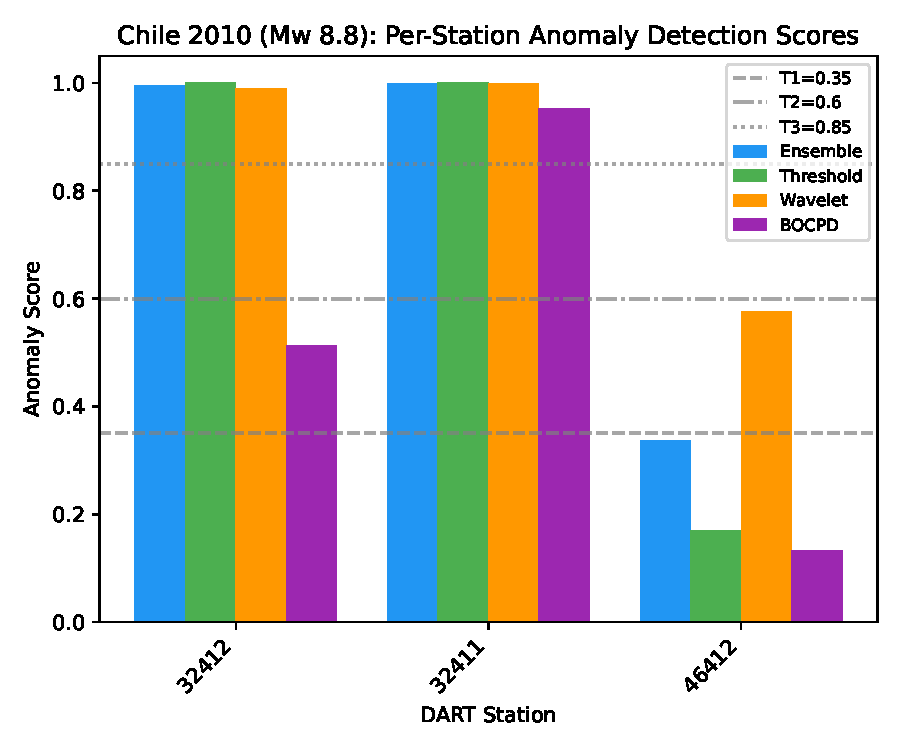
\includegraphics[width=\linewidth]{figures/fig_chile_detection.pdf}
\caption{Chile 2010 per-station anomaly scores (event-mode stations only).
  Horizontal lines indicate FSM thresholds $T_1$, $T_2$, $T_3$.
  Two of the three event-mode stations (32411, 32412) exceed $T_1$
  and $T_3$; 46412 peaks just below $T_1$ on the full window.  Standard-mode stations are omitted because bandpass filter
  degradation at 15-min sampling renders scores unreliable
  (see Table~\ref{tab:chile-results}).}
\label{fig:chile-detection}
\end{figure}

\begin{figure}[!htbp]
\centering
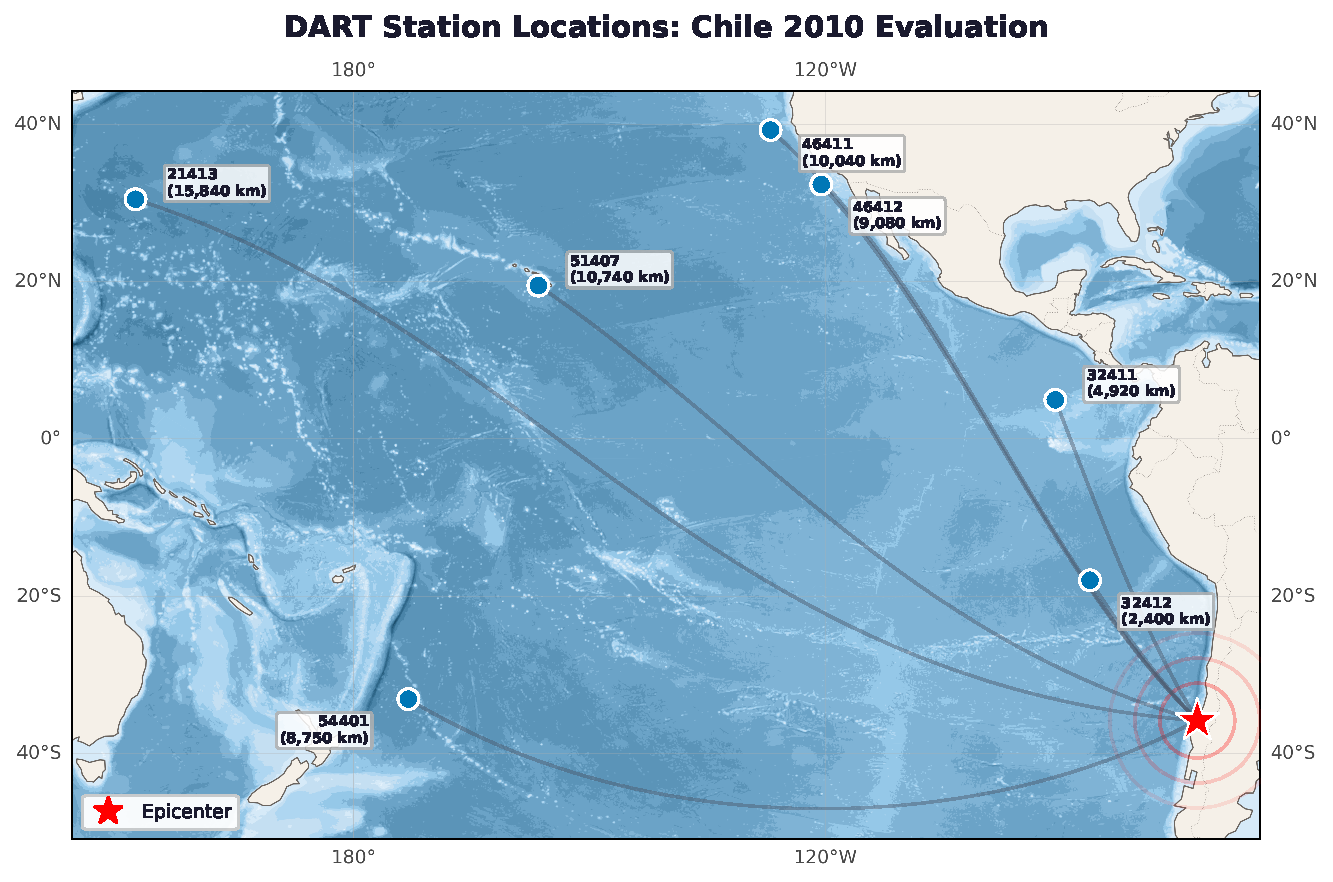
\includegraphics[width=\linewidth]{figures/fig_chile_station_map.pdf}
\caption{DART station locations used for Chile 2010
  evaluation, with epicenter (red star) and epicentral
  distances.  Stations span from 2{,}400\,km (32412, off Peru) to
  15{,}840\,km (21413, off Japan).}
\label{fig:chile-station-map}
\end{figure}

\begin{figure}[!htbp]
\centering
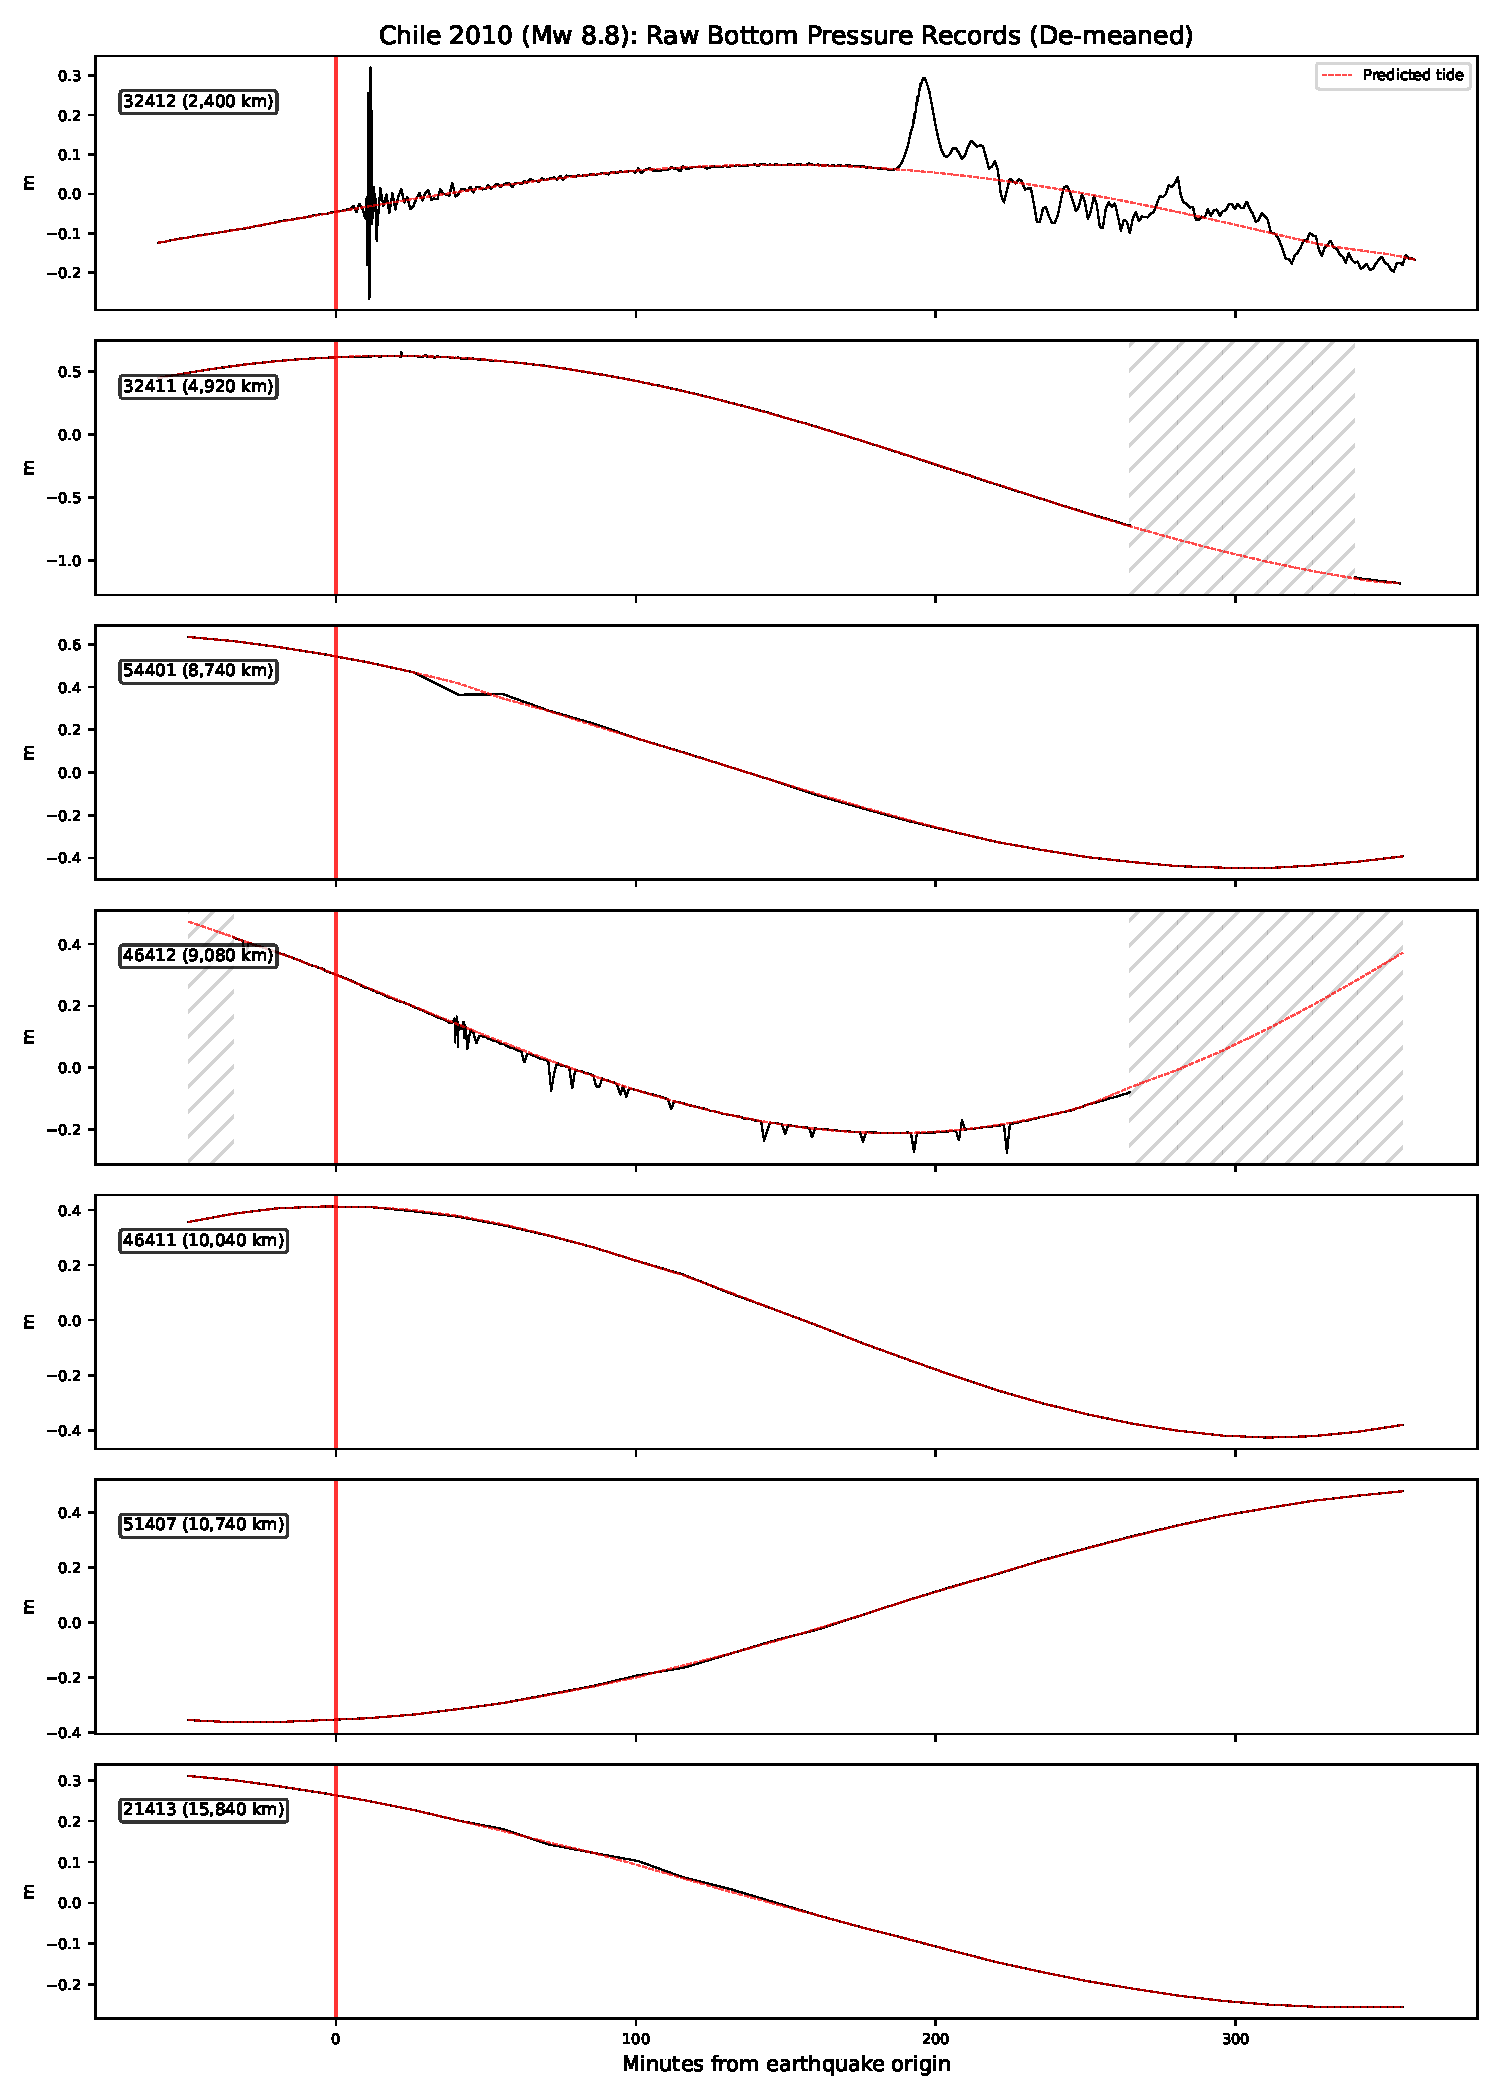
\includegraphics[width=0.92\linewidth]{figures/fig_chile_waveforms.pdf}
\caption{Chile 2010 raw bottom pressure records (de-meaned), ordered by
  epicentral distance.  Red vertical line marks earthquake origin.
  Standard-mode stations (54401, 46411, 51407, 21413) show 15-min
  sampling; event-mode stations (32412, 32411, 46412) show 1-min
  sampling.  Red dashed: IRLS tidal prediction.
  Hatched regions indicate data gaps.}
\label{fig:chile-waveforms}
\end{figure}

\begin{figure}[!htbp]
\centering
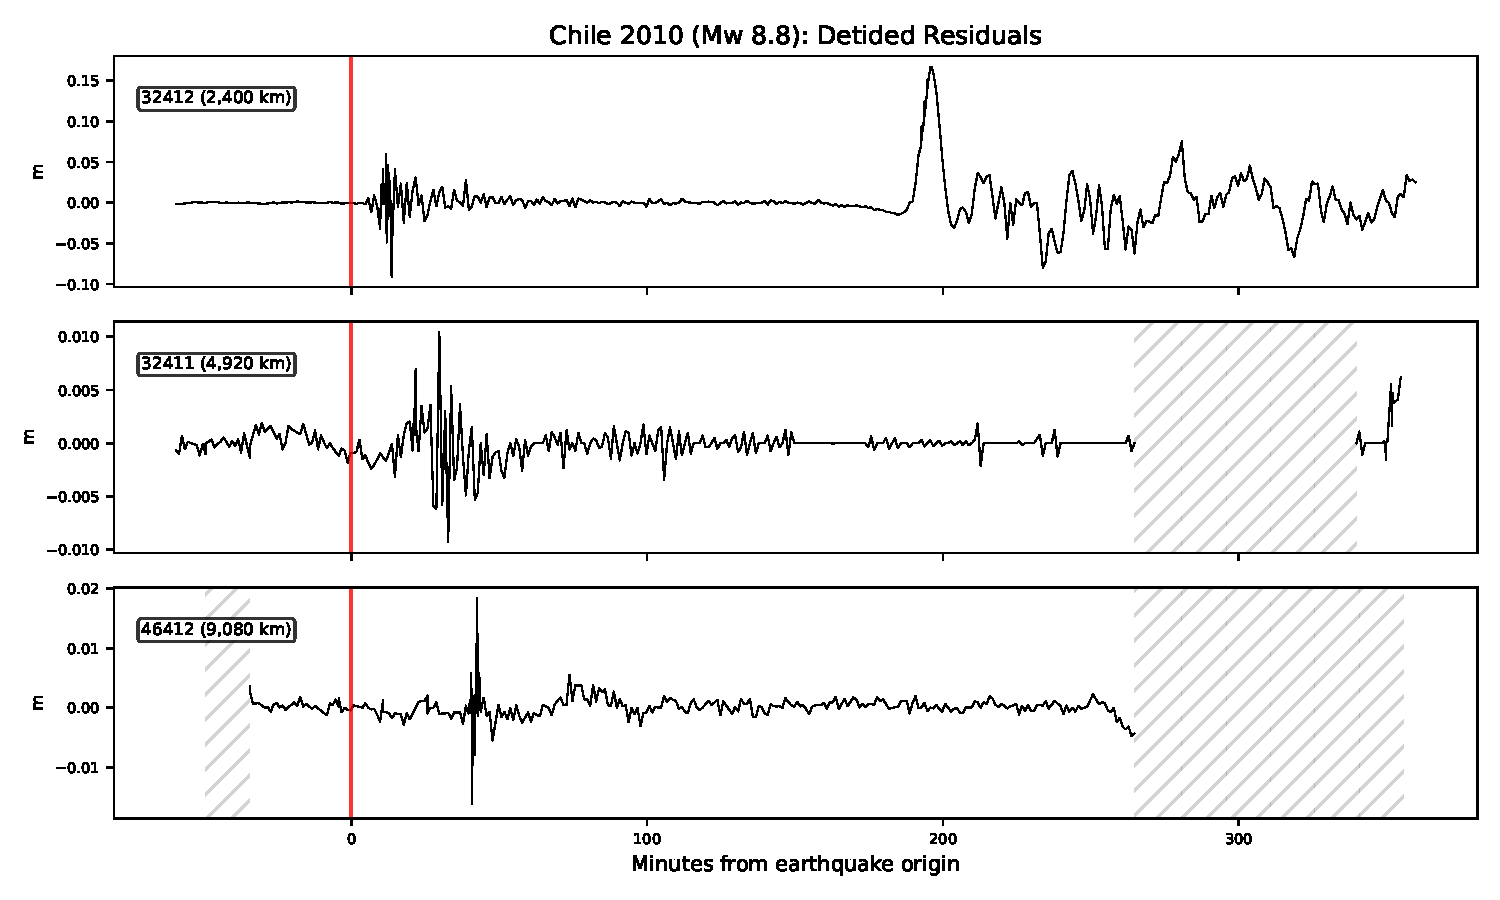
\includegraphics[width=0.92\linewidth]{figures/fig_chile_residuals.pdf}
\caption{Chile 2010 detided residuals (tsunami waveform) after harmonic
  tidal removal for the three DART stations that operated in event mode
  (1-min sampling).  Four additional far-field stations remained in
  standard mode (15-min sampling, 28 points) and are omitted because
  their coarse resolution precludes reliable detiding.  Processing:
  despike, pre-event linear detrend, 60-min centered rolling median,
  Hampel filter (Algorithm~\ref{alg:residual}).}
\label{fig:chile-residuals}
\end{figure}

\begin{figure}[!htbp]
\centering
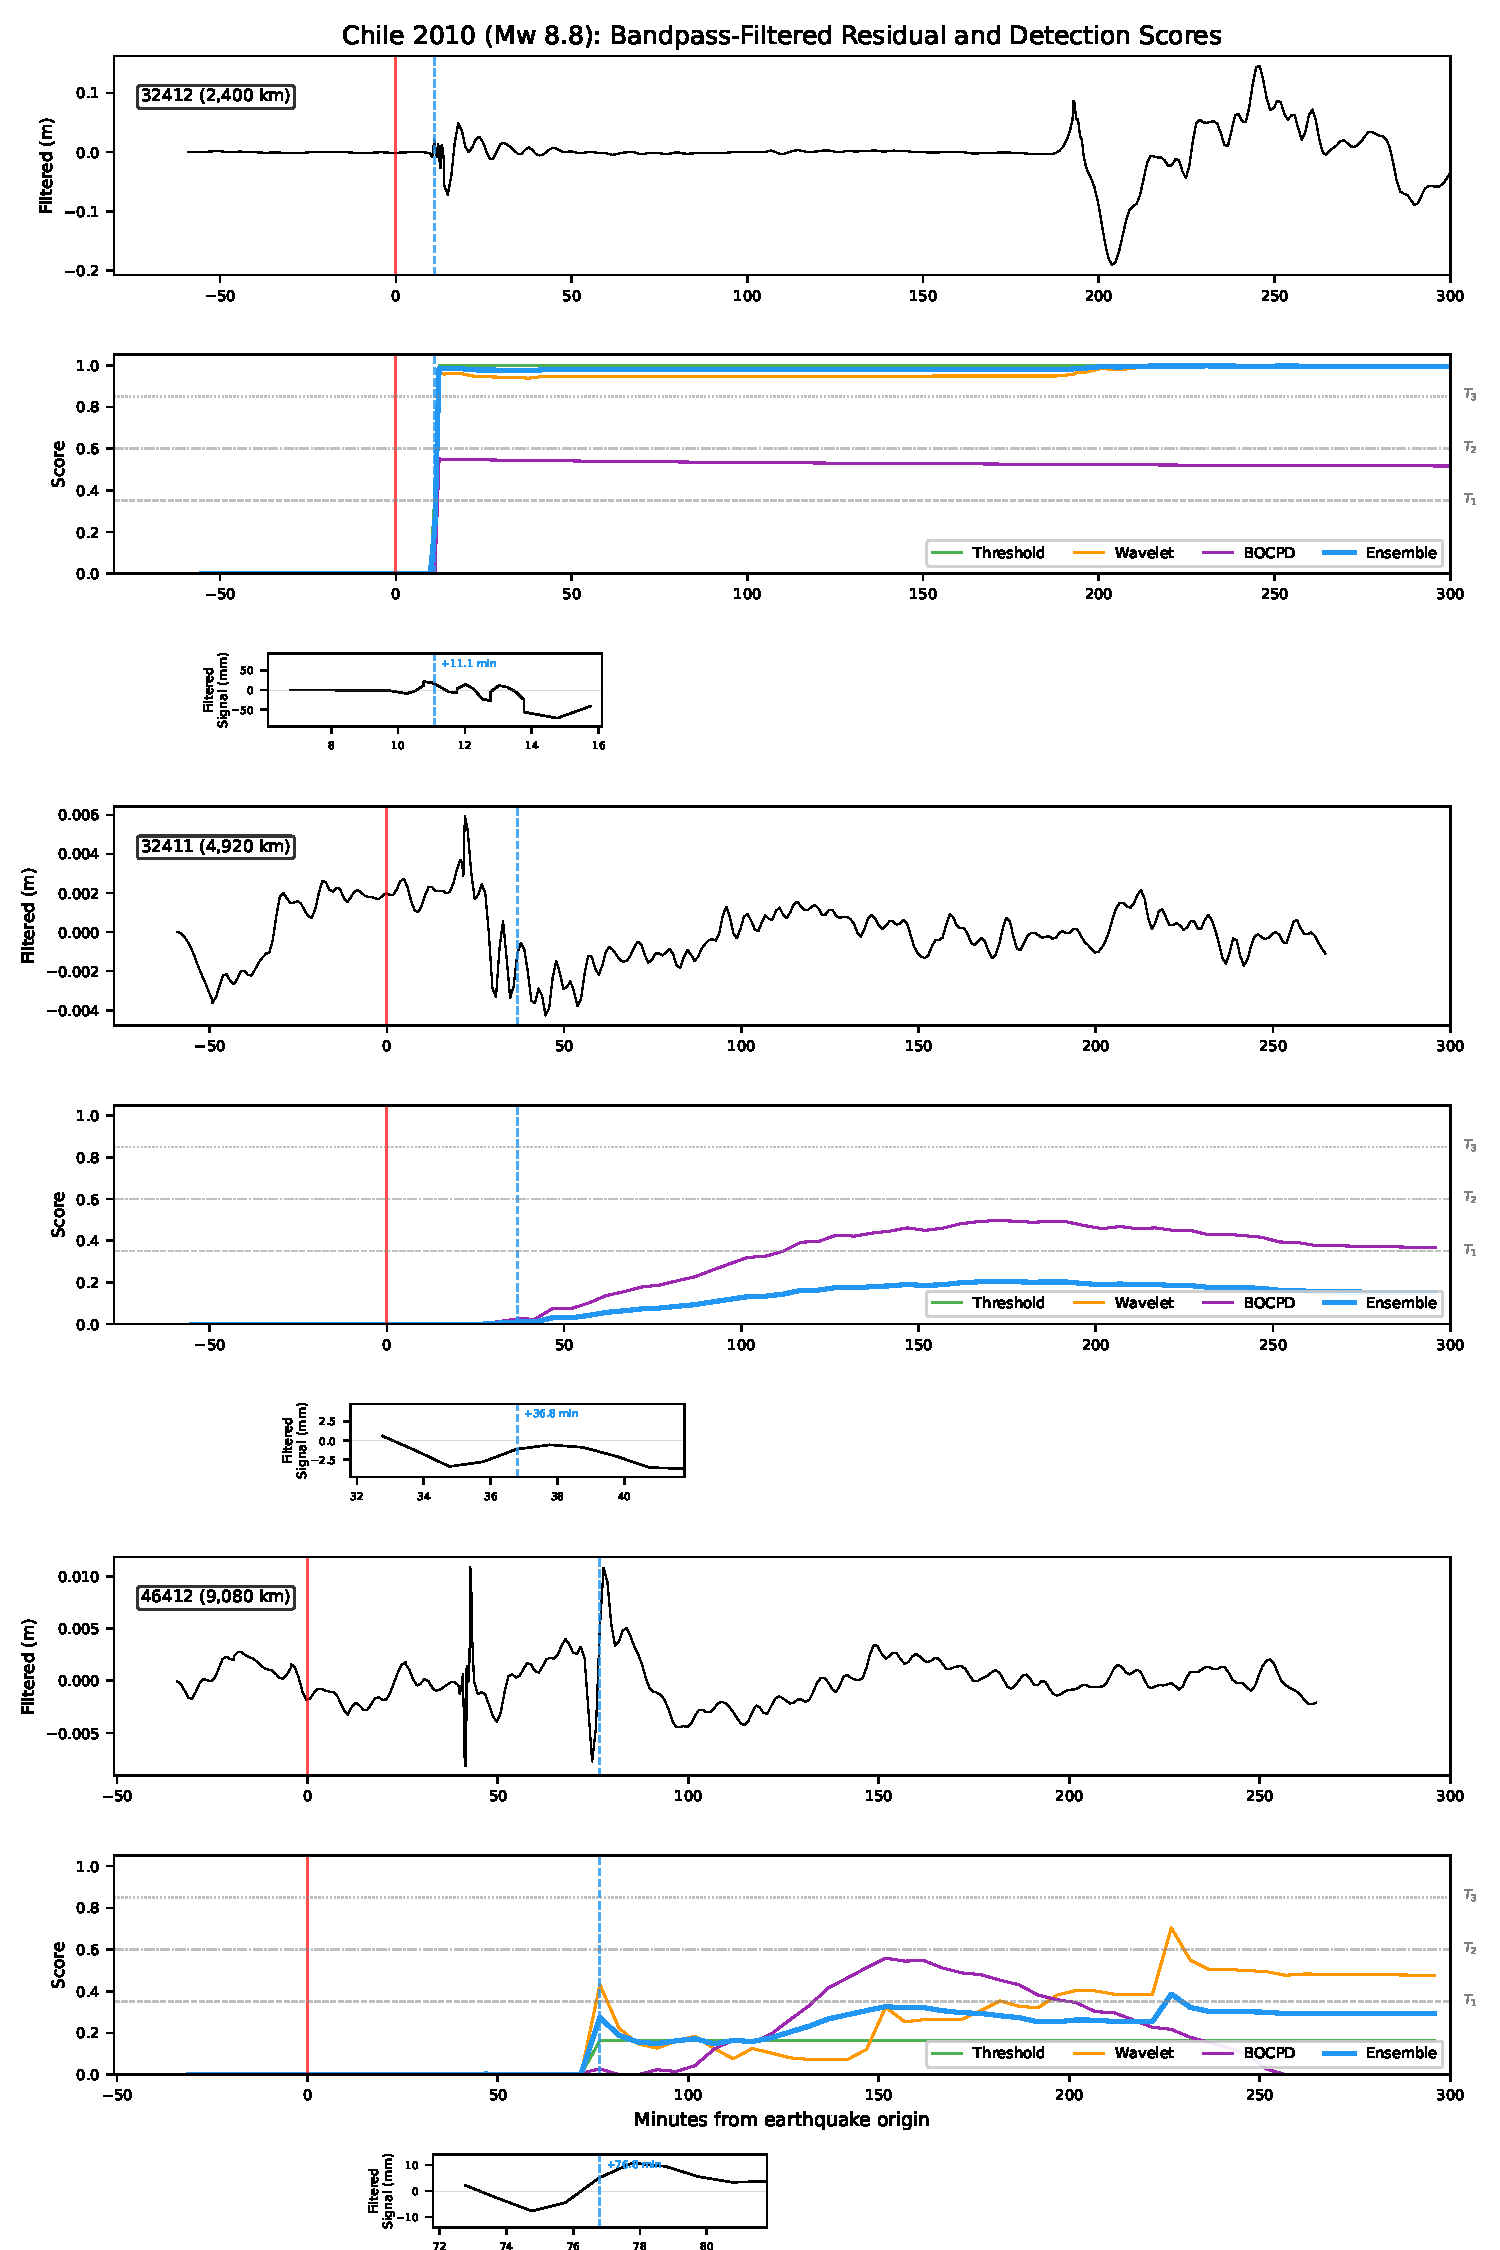
\includegraphics[width=\linewidth]{figures/fig_chile_detection_timeline.pdf}
\caption{Detection pipeline signals and scores for Chile 2010
  event-mode stations (matching Figure~\ref{fig:score-overlay} format).
  For each station: (top) bandpass-filtered detided residual
  (5--120\,min passband, causal Butterworth),
  (bottom) component and ensemble scores from sliding-window analysis
  with FSM thresholds $T_1$, $T_2$, $T_3$.
  Insets below each score panel show the signal at mm scale around
  score onset, the first nonzero ensemble score (blue dashed line).
  Station 32412 (2{,}400\,km) crosses $T_1$ through $T_3$ at
  +12.3\,min from seismic energy;
  station 32411 (4{,}920\,km) shows gradual BOCPD buildup;
  station 46412 (9{,}080\,km) shows only a transient late crossing
  (+226.8\,min) that does not persist over the full window.}
\label{fig:chile-timeline}
\end{figure}

\FloatBarrier
\subsection{Illapel 2015 Magnitude-Range Validation}
\label{sec:eval-illapel}

To test detection sensitivity at a lower magnitude, we apply the
pipeline to the 2015 Illapel $M_w$\,8.3 earthquake
(2015-09-16 22:54:32 UTC; 31.573\textdegree S, 71.674\textdegree W;
depth 22\,km; USGS event us20003k7a).
Seven DART stations spanning 580--12{,}450\,km are selected
(Table~\ref{tab:illapel-stations}); stations 46411 and 46403
overlap with the T\={o}hoku evaluation.

\begin{table}[!htb]
\centering
\caption{DART stations used in the Illapel 2015 retrospective validation.
  Distances from the epicenter (31.573\textdegree S, 71.674\textdegree W)
  computed via haversine.}
\label{tab:illapel-stations}
\small
\begin{tabular}{lrll}
\toprule
\textbf{Station} & \textbf{Dist.\,(km)} & \textbf{Location} & \textbf{Mode} \\
\midrule
32402 &    580  & W of Caldera, Chile    & event (1\,min) \\
32401 & 1{,}230 & W of Iquique, Chile    & event (1\,min) \\
32412 & 2{,}110 & NW, off Peru           & event (1\,min) \\
51426 & 9{,}260 & W, near Tonga          & standard (15\,min) \\
46411 & 9{,}740 & N, off N California    & standard (15\,min) \\
46407 & 10{,}110 & N, off Oregon          & standard (15\,min) \\
46403 & 12{,}450 & NNE, off Alaska        & standard (15\,min) \\
\bottomrule
\end{tabular}
\end{table}

Three near-field stations (32402, 32401, 32412) operated in DART
event mode (1-min sampling) during the event window
(Figure~\ref{fig:illapel-detection}).
The closest station (32402 at 580\,km) produced an ensemble score of
0.99, comfortably exceeding the ESCALATE threshold ($T_3 = 0.85$);
station 32401 at 1{,}230\,km scored 0.753 (ASSESS level, $T_2 = 0.60$).
Station 32412, at 2{,}110\,km, scored 0.49 (above INVESTIGATE
threshold $T_1 = 0.35$), consistent with its greater distance
and the smaller source amplitude compared to the $M_w$\,8.8--9.1
events.  The four far-field stations remained in 15-min standard
mode within the 6-hour event window; their filter-degraded scores
are reported but not used for detection assessment.
Table~\ref{tab:illapel-results} provides the full per-station breakdown.
Raw pressure records with IRLS tidal fits are shown in
Figure~\ref{fig:illapel-waveforms}; detided residuals in
Figure~\ref{fig:illapel-residuals}; station geometry in
Figure~\ref{fig:illapel-station-map}; detection score timelines in
Figure~\ref{fig:illapel-timeline}.
CO-OPS water-level records are shown in
Appendix~\ref{sec:appendix-coops} (Figure~\ref{fig:coops-illapel}).

\noindent\textbf{Agentic pipeline trace.}
At $M_w$\,8.3 and 22\,km depth, seismic-only escalation fires
immediately.  DART evidence arrives at +3.7\,min when
station 32402 (580\,km) crosses $T_1$.  Station 32402 reaches
$T_3$ at +5.0\,min; station 32401 (1{,}230\,km) reaches
$T_2$ but not $T_3$ (ensemble 0.753), demonstrating the
ensemble's graded response at intermediate distances.
Audit trail:
(1)~\texttt{state\_transition}: IDLE~$\to$~MONITOR ($M$\,8.3);
(2)~\texttt{state\_transition}: MONITOR~$\to$~ESCALATE
(seismic-only, 22\,km);
(3)~\texttt{verification\_complete}: PASS\_WITH\_CONCERNS
(3 stations above $T_1$);
(4)~\texttt{report\_generated}: Tier~1, PROVISIONAL.

\begin{table}[!htb]
\centering
\caption{Illapel 2015 per-station anomaly detection results.
  Column definitions match Table~\ref{tab:tohoku-results}.}
\label{tab:illapel-results}
\footnotesize
\begin{tabular}{lrccccccccc}
\toprule
\textbf{Station} & \textbf{Dist (km)} & \textbf{Mode}
  & \textbf{Ens.} & \textbf{Thr.} & \textbf{Wav.}
  & \textbf{BCP} & \textbf{INV} & \textbf{ASS} & \textbf{ESC}
  & \textbf{Deg} \\
\midrule
32402 &    580    & event & 0.992 & 1.000 & 0.981 & 0.304 & \checkmark & \checkmark & \checkmark & --- \\
32401 & 1{,}230   & event & 0.753 & 0.914 & 0.524 & 0.364 & \checkmark & \checkmark & ---        & --- \\
32412 & 2{,}110   & event & 0.493 & 0.539 & 0.120 & 0.427 & \checkmark & ---        & ---        & --- \\
51426 & 9{,}260   & std   & 0.000 & 0.000 & 0.000 & 0.000 & ---        & ---        & ---        & \checkmark \\
46411 & 9{,}740   & std   & 0.000 & 0.000 & 0.000 & 0.000 & ---        & ---        & ---        & \checkmark \\
46407 & 10{,}110  & std   & 0.000 & 0.000 & 0.000 & 0.000 & ---        & ---        & ---        & \checkmark \\
46403 & 12{,}450  & std   & 0.000 & 0.000 & 0.000 & 0.001 & ---        & ---        & ---        & \checkmark \\
\bottomrule
\end{tabular}
\end{table}

\begin{figure}[!htbp]
\centering
\begin{subfigure}[t]{0.52\linewidth}
  \centering
  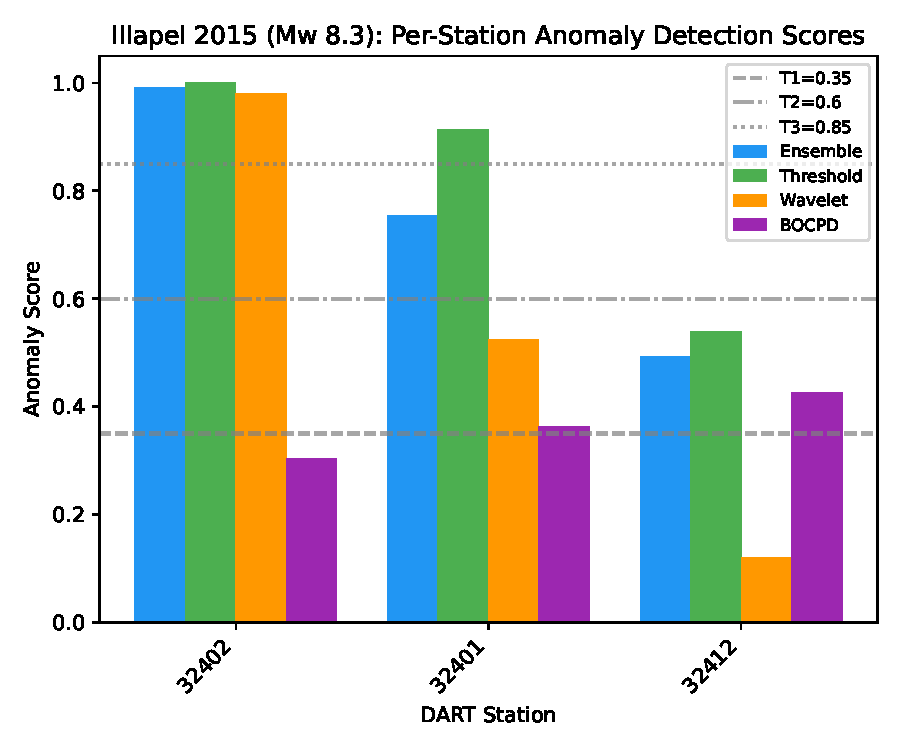
\includegraphics[width=\linewidth]{figures/fig_illapel_detection.pdf}
  \caption{Per-station anomaly scores (event-mode only).}
  \label{fig:illapel-detection}
\end{subfigure}\hfill
\begin{subfigure}[t]{0.46\linewidth}
  \centering
  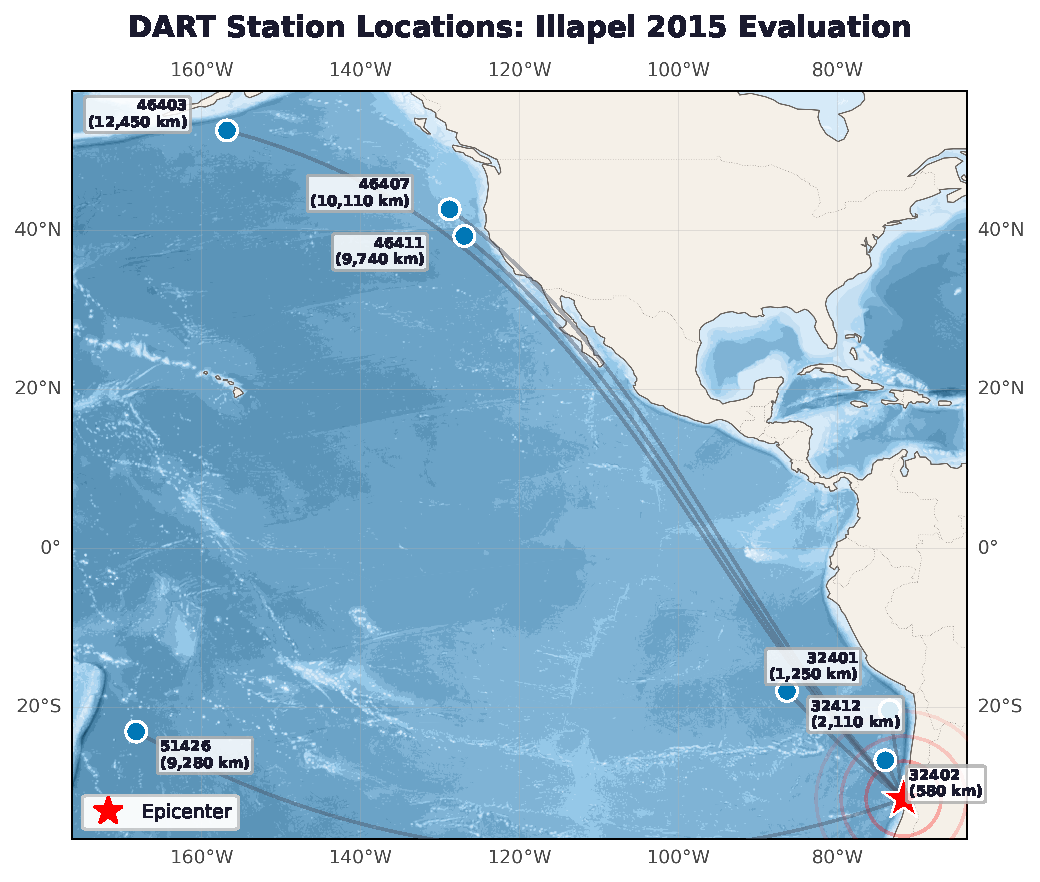
\includegraphics[width=\linewidth]{figures/fig_illapel_station_map.pdf}
  \caption{DART station locations; red star marks epicenter.}
  \label{fig:illapel-station-map}
\end{subfigure}
\caption{Illapel 2015 ($M_w$ 8.3) detection results and station geometry.
  (a) 32402 exceeds ESCALATE; 32401 exceeds ASSESS; 32412 exceeds INVESTIGATE.
  Standard-mode stations omitted (Table~\ref{tab:illapel-results}).
  (b) Epicenter at 31.573\textdegree S, 71.674\textdegree W.}
\end{figure}

This result demonstrates detection capability at $M_w$\,8.3, extending
the validated magnitude range below the $M_w$\,8.8 Chile 2010 event.

\begin{figure}[!htbp]
\centering
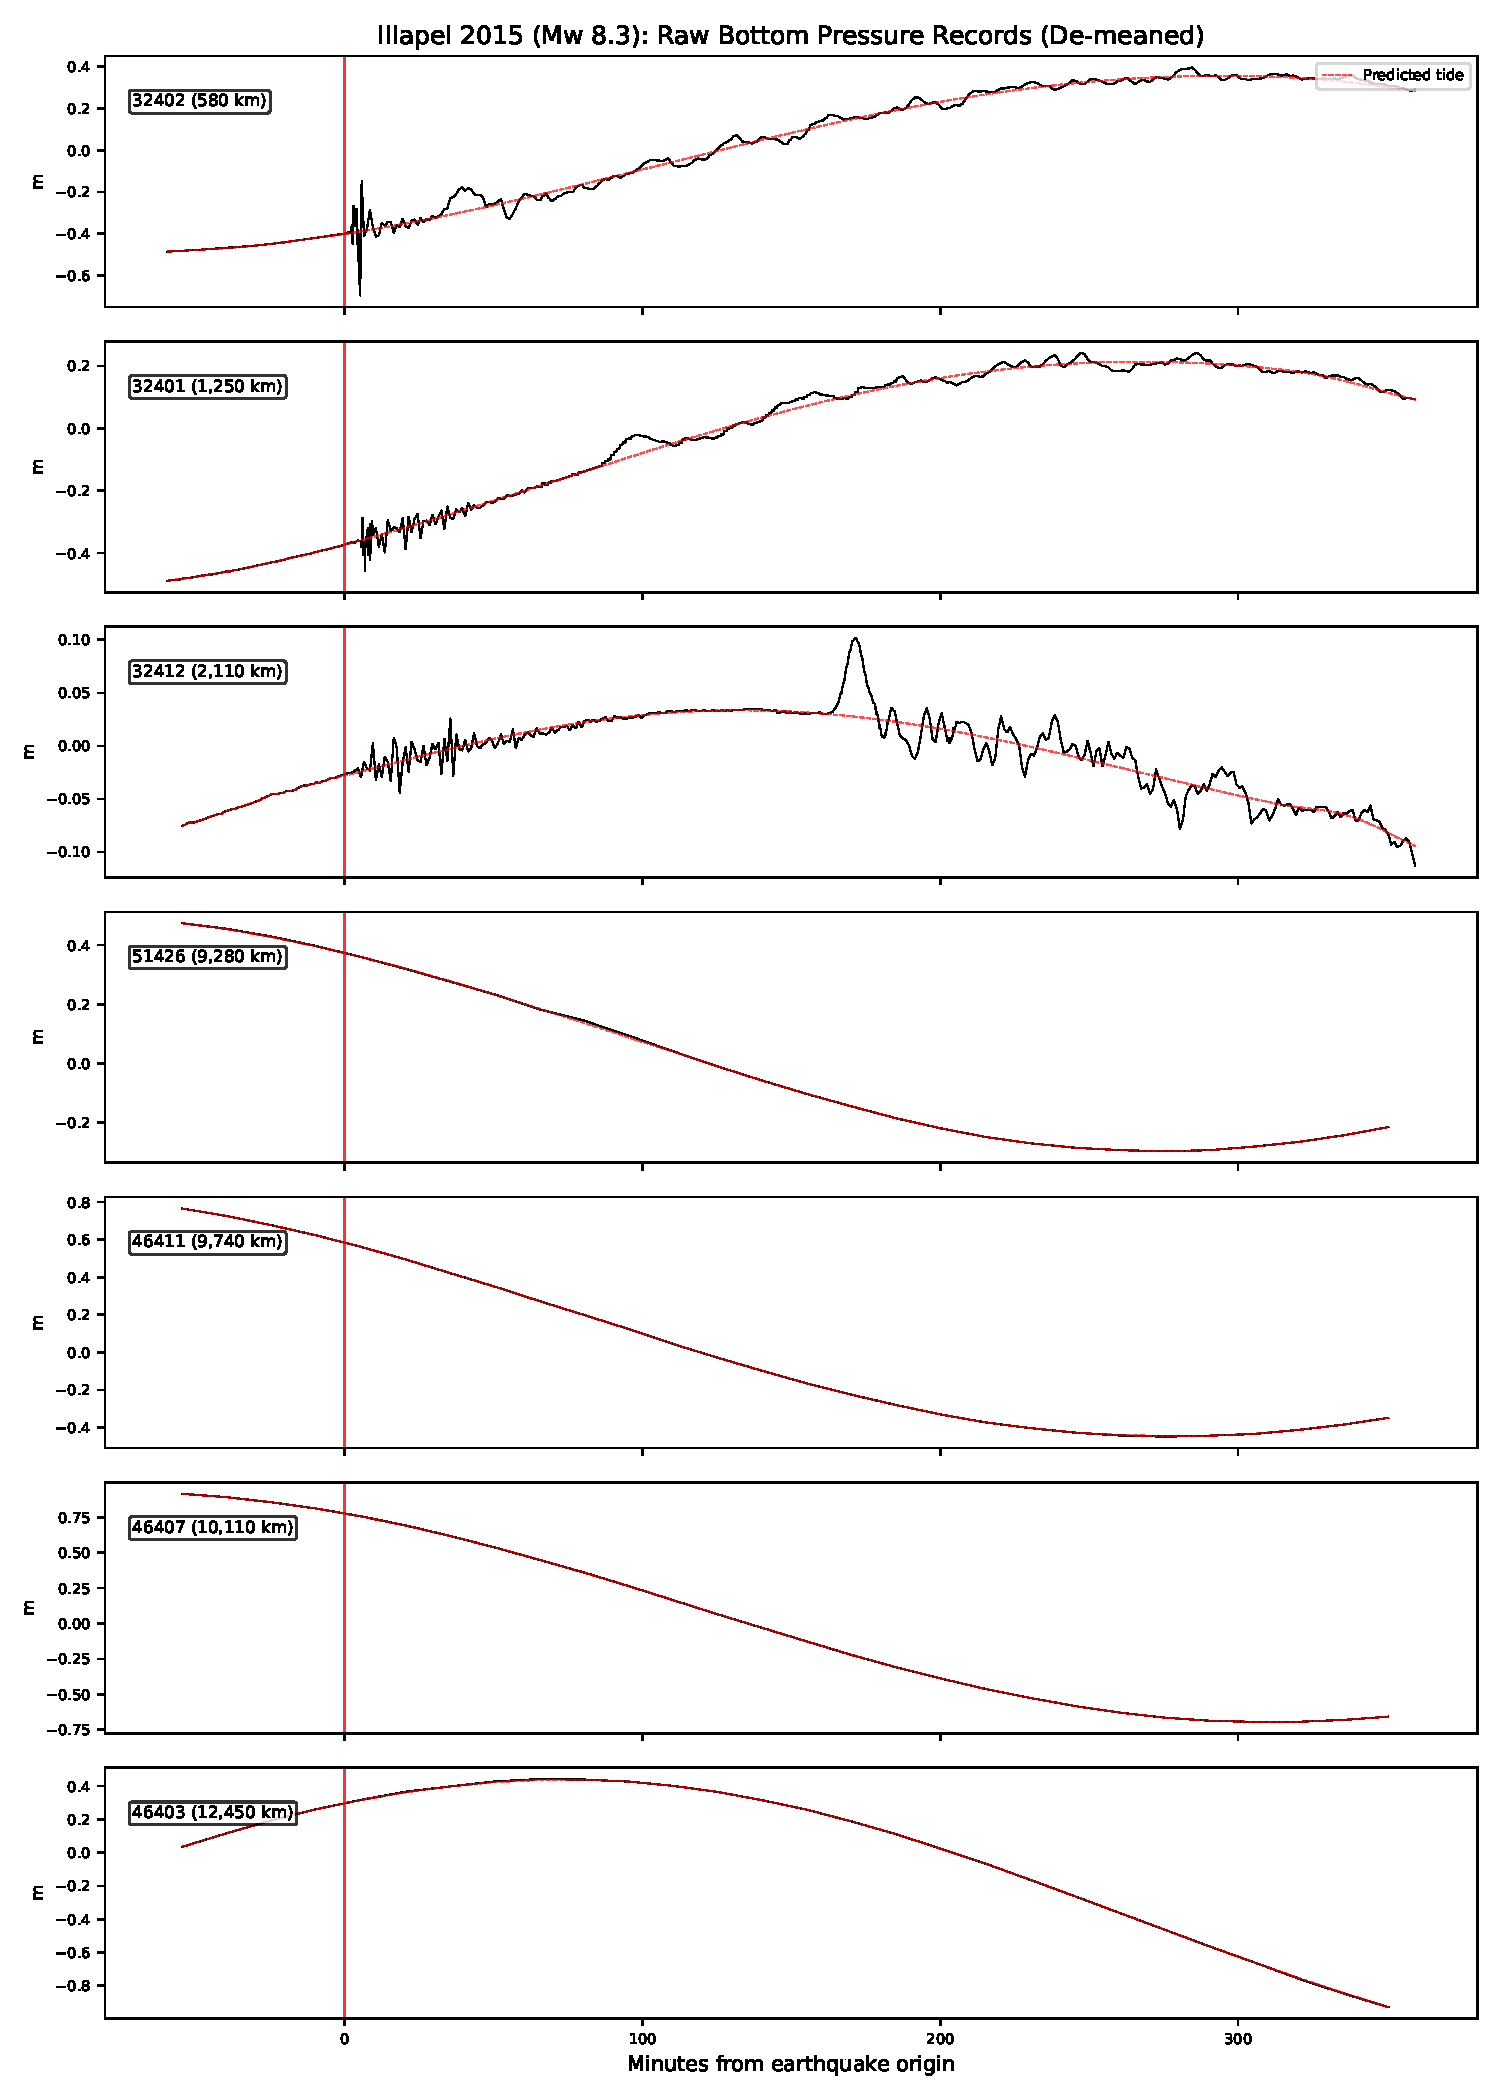
\includegraphics[width=0.92\linewidth]{figures/fig_illapel_waveforms.pdf}
\caption{Illapel 2015: raw bottom pressure records (de-meaned) for
  all seven DART stations, ordered by epicentral distance.
  Red dashed: IRLS tidal prediction.
  Hatched regions indicate data gaps.}
\label{fig:illapel-waveforms}
\end{figure}

\begin{figure}[!htbp]
\centering
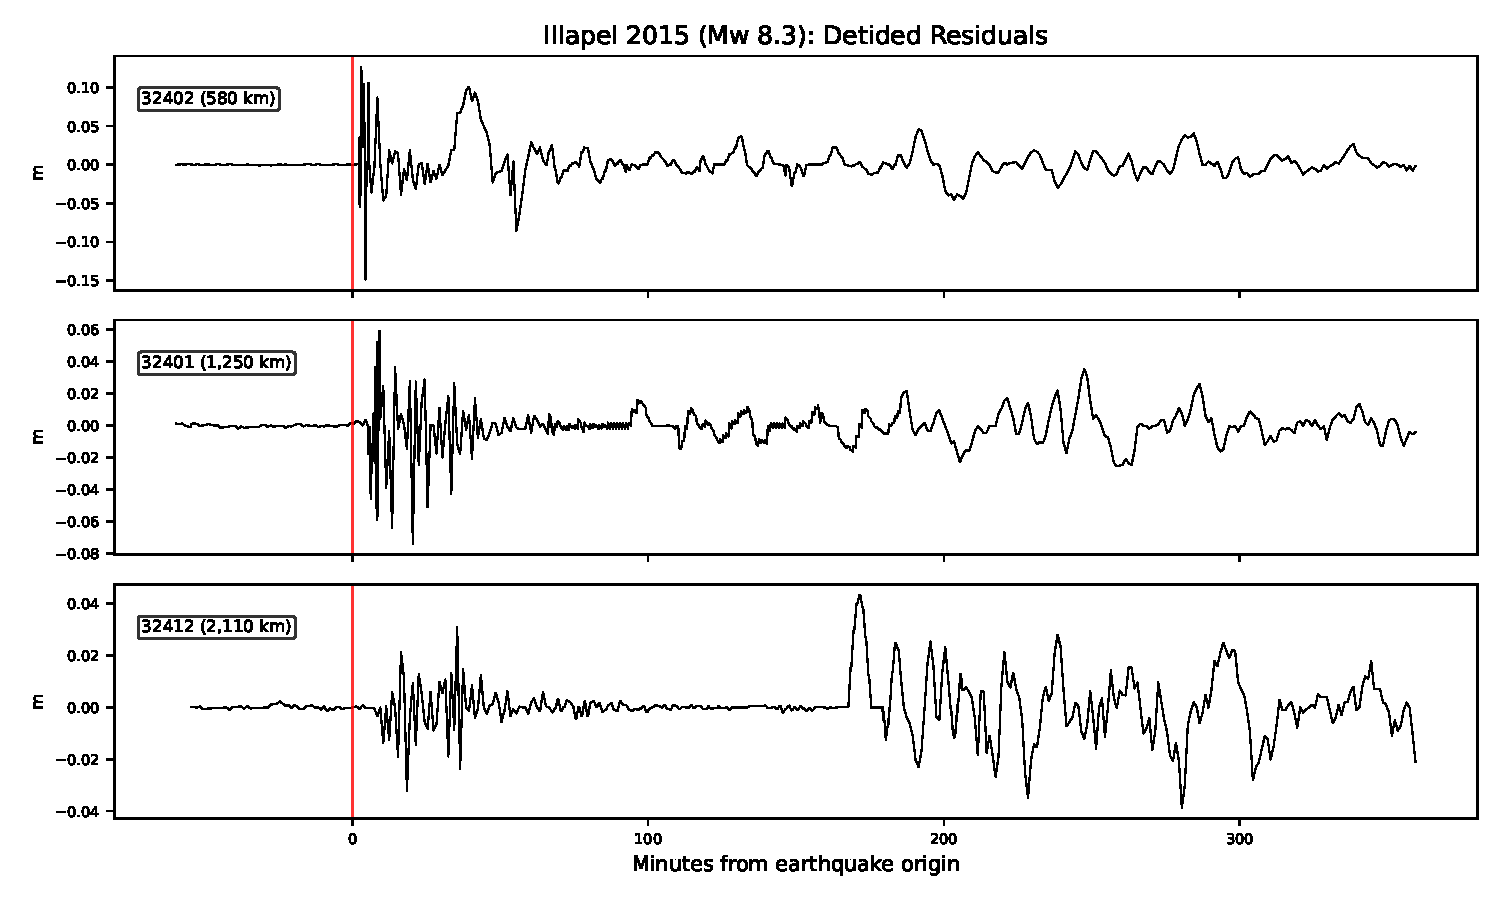
\includegraphics[width=0.92\linewidth]{figures/fig_illapel_residuals.pdf}
\caption{Illapel 2015: detided residuals for the three event-mode
  stations.  Despike, pre-event linear detrend, 30-min centered
  rolling median, and Hampel spike filter applied
  (Algorithm~\ref{alg:residual}).}
\label{fig:illapel-residuals}
\end{figure}

\begin{figure}[!htbp]
\centering
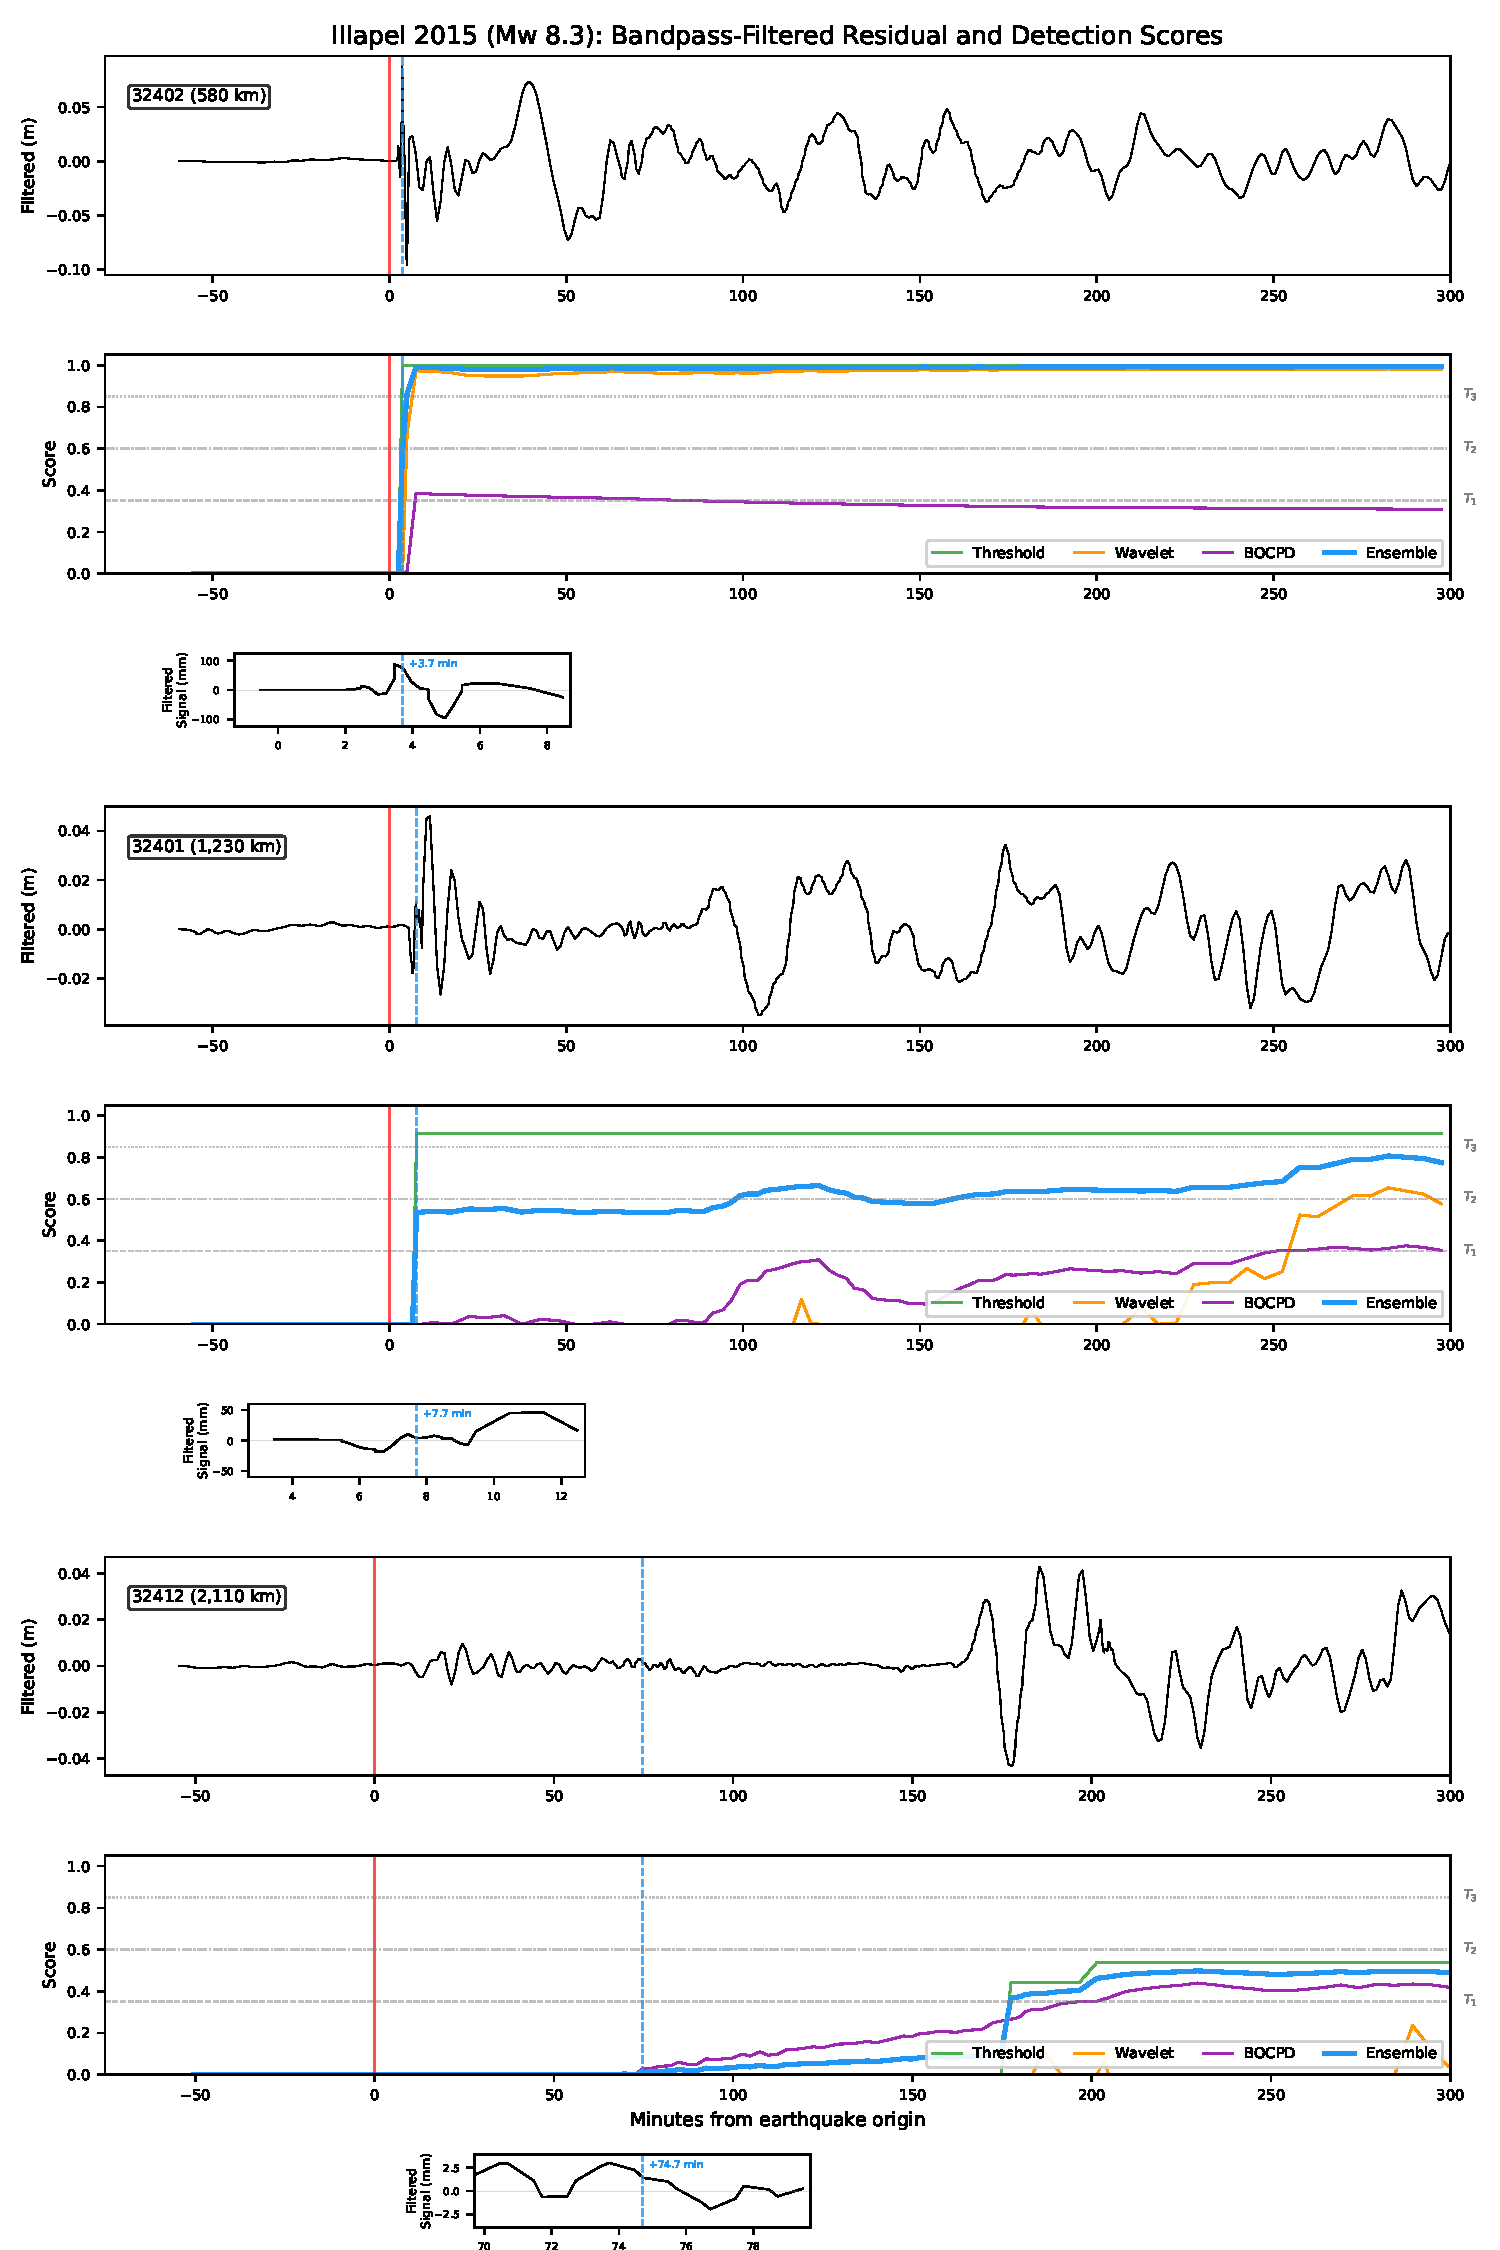
\includegraphics[width=\linewidth,height=0.85\textheight,keepaspectratio]{figures/fig_illapel_detection_timeline.pdf}
\caption{Detection pipeline signals and scores for Illapel 2015
  event-mode stations (matching Figure~\ref{fig:score-overlay} format).
  For each station: (top) bandpass-filtered detided residual
  (5--120\,min passband, causal Butterworth),
  (bottom) component and ensemble scores from sliding-window analysis
  with FSM thresholds $T_1$, $T_2$, $T_3$.
  Insets below each score panel show the signal at mm scale around
  score onset, the first nonzero ensemble score (blue dashed line).}
\label{fig:illapel-timeline}
\end{figure}

\FloatBarrier
\subsection{Iquique 2014 Validation}
\label{sec:eval-iquique}

To further extend the magnitude range, we evaluate the 2014 Iquique
$M_w$\,8.2 earthquake (2014-04-01 23:46:47 UTC; 19.610\textdegree S,
70.769\textdegree W; depth 25\,km; USGS event usc000nzvd).
Six DART stations are selected (Table~\ref{tab:iquique-stations});
four operated in event mode during the event window.

\begin{table}[!htb]
\centering
\caption{DART stations used in the Iquique 2014 retrospective validation
  (epicenter 19.610\textdegree{}S, 70.769\textdegree{}W).
  Distances computed via haversine. The interval given for an
  event-mode station is the median spacing of its retained record, not
  an instrument setting. These records interleave samples that the
  NDBC archive tags as 15-second and 1-minute mode, and the median
  lands at 45\,s on the two stations that kept the most 15-second
  samples, 120 and 103 against 25 and 20 on the other two. The
  per-sample mode is preserved in the native records under
  \texttt{data/iquique/native/}, whose manifest documents the tag.}
\label{tab:iquique-stations}
\small
\begin{tabular}{lrll}
\toprule
\textbf{Station} & \textbf{Dist.\,(km)} & \textbf{Location} & \textbf{Mode} \\
\midrule
32401 &    295  & SSW, off Arica, Chile   & event (1\,min) \\
32402 &    858  & S, off Caldera, Chile   & event (1\,min) \\
32412 & 1{,}652 & NW, off Peru            & event (45\,s) \\
32413 & 2{,}809 & NW, off Peru (far)      & event (45\,s) \\
51426 & 9{,}900 & W, near Tonga           & standard (15\,min) \\
46403 & 11{,}476 & NNE, off Alaska        & standard (15\,min) \\
\bottomrule
\end{tabular}
\end{table}

All four event-mode stations exceed the INVESTIGATE threshold
(Figure~\ref{fig:iquique-detection}).
The two nearest (32401, 32402) score 0.70 and 0.82 (ASSESS);
the two more distant stations (32412, 32413) score 0.98 and 1.00,
both exceeding ESCALATE.  The higher scores at 32412 and 32413
compared to the nearer stations reflect stronger wavelet responses
at those stations. The two far-field standard-mode stations
(51426, 46403) show filter degradation and produce zero scores.
Station 32413 had only ${\sim}5.9$~days of pre-event calibration data
available in the NDBC archive (vs.\ the nominal 30~days); despite the
shortened tidal fit window, it achieved the highest ensemble score
(1.00) among the four event-mode stations.
Table~\ref{tab:iquique-results} provides the full per-station breakdown.
Raw pressure records with IRLS tidal fits are shown in
Figure~\ref{fig:iquique-waveforms}; detided residuals in
Figure~\ref{fig:iquique-residuals}; station geometry in
Figure~\ref{fig:iquique-station-map}; detection score timelines in
Figure~\ref{fig:iquique-timeline}.
CO-OPS water-level records are shown in
Appendix~\ref{sec:appendix-coops} (Figure~\ref{fig:coops-iquique}).

\noindent\textbf{Agentic pipeline trace.}
Seismic-only escalation fires at $M_w$\,8.2, depth 25\,km.
DART evidence shows a longer progression: station 32401
crosses $T_1$ at +2.7\,min, but $T_3$ is not reached until
station 32412 at +141.2\,min.  This 2.3-hour delay between
initial detection and full escalation threshold illustrates
the value of the two-phase architecture: seismic-only
escalation places the event in front of the duty scientist
immediately, while DART-based scoring accumulates over time.
Audit trail:
(1)~\texttt{state\_transition}: IDLE~$\to$~MONITOR ($M$\,8.2);
(2)~\texttt{state\_transition}: MONITOR~$\to$~ESCALATE
(seismic-only, 25\,km);
(3)~\texttt{verification\_complete}: PASS\_WITH\_CONCERNS
(4 stations above $T_1$);
(4)~\texttt{report\_generated}: Tier~1, PROVISIONAL.

\begin{table}[!htb]
\centering
\caption{Iquique 2014 per-station anomaly detection results.
  Column definitions match Table~\ref{tab:tohoku-results}.
  Station 32413 had only ${\sim}5.9$~days of calibration data.}
\label{tab:iquique-results}
\footnotesize
\begin{tabular}{lrccccccccc}
\toprule
\textbf{Station} & \textbf{Dist (km)} & \textbf{Mode}
  & \textbf{Ens.} & \textbf{Thr.} & \textbf{Wav.}
  & \textbf{BCP} & \textbf{INV} & \textbf{ASS} & \textbf{ESC}
  & \textbf{Deg} \\
\midrule
32401 &    295    & event & 0.698 & 1.000 & 0.000 & 0.266 & \checkmark & \checkmark & ---        & --- \\
32402 &    858    & event & 0.817 & 1.000 & 0.000 & 0.557 & \checkmark & \checkmark & ---        & --- \\
32412 & 1{,}652   & event & 0.978 & 0.986 & 0.965 & 0.000 & \checkmark & \checkmark & \checkmark & --- \\
32413 & 2{,}809   & event & 1.000 & 1.000 & 1.000 & 0.932 & \checkmark & \checkmark & \checkmark & --- \\
51426 & 9{,}900   & std   & 0.000 & 0.000 & 0.000 & 0.000 & ---        & ---        & ---        & \checkmark \\
46403 & 11{,}476  & std   & 0.000 & 0.000 & 0.000 & 0.000 & ---        & ---        & ---        & \checkmark \\
\bottomrule
\end{tabular}
\end{table}

\begin{figure}[!htbp]
\centering
\begin{subfigure}[t]{0.52\linewidth}
  \centering
  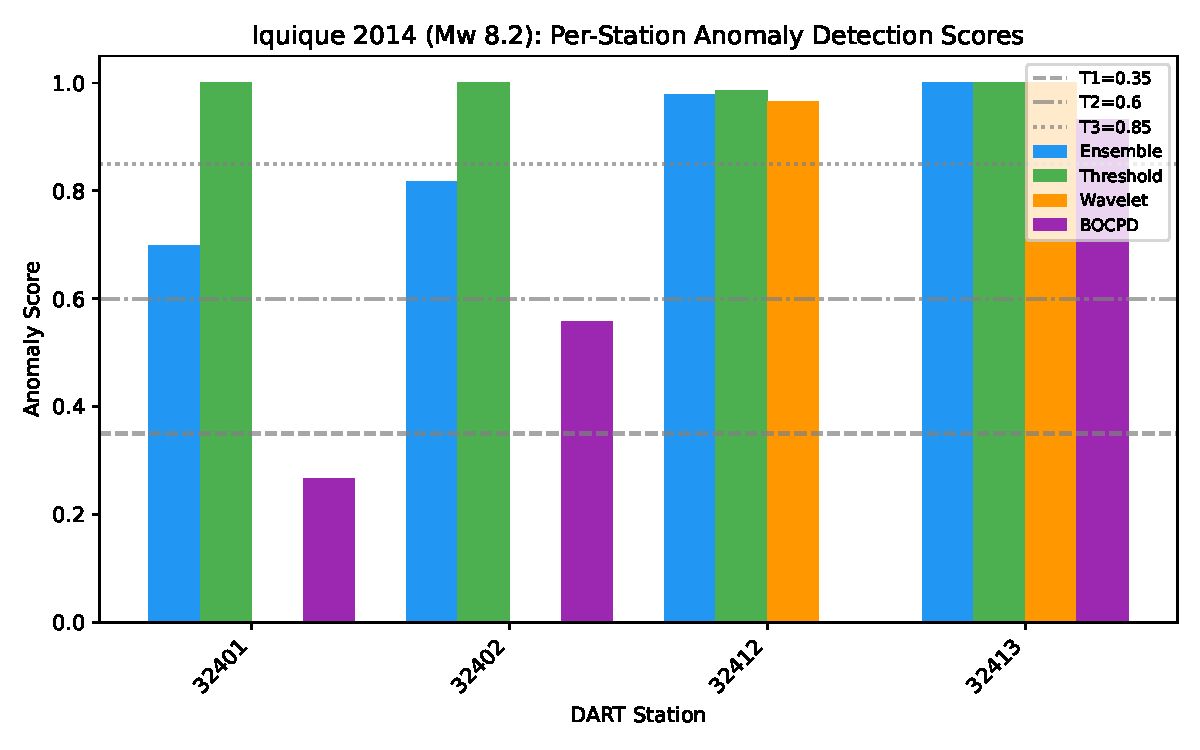
\includegraphics[width=\linewidth]{figures/fig_iquique_detection.pdf}
  \caption{Per-station anomaly scores (event-mode only).}
  \label{fig:iquique-detection}
\end{subfigure}\hfill
\begin{subfigure}[t]{0.46\linewidth}
  \centering
  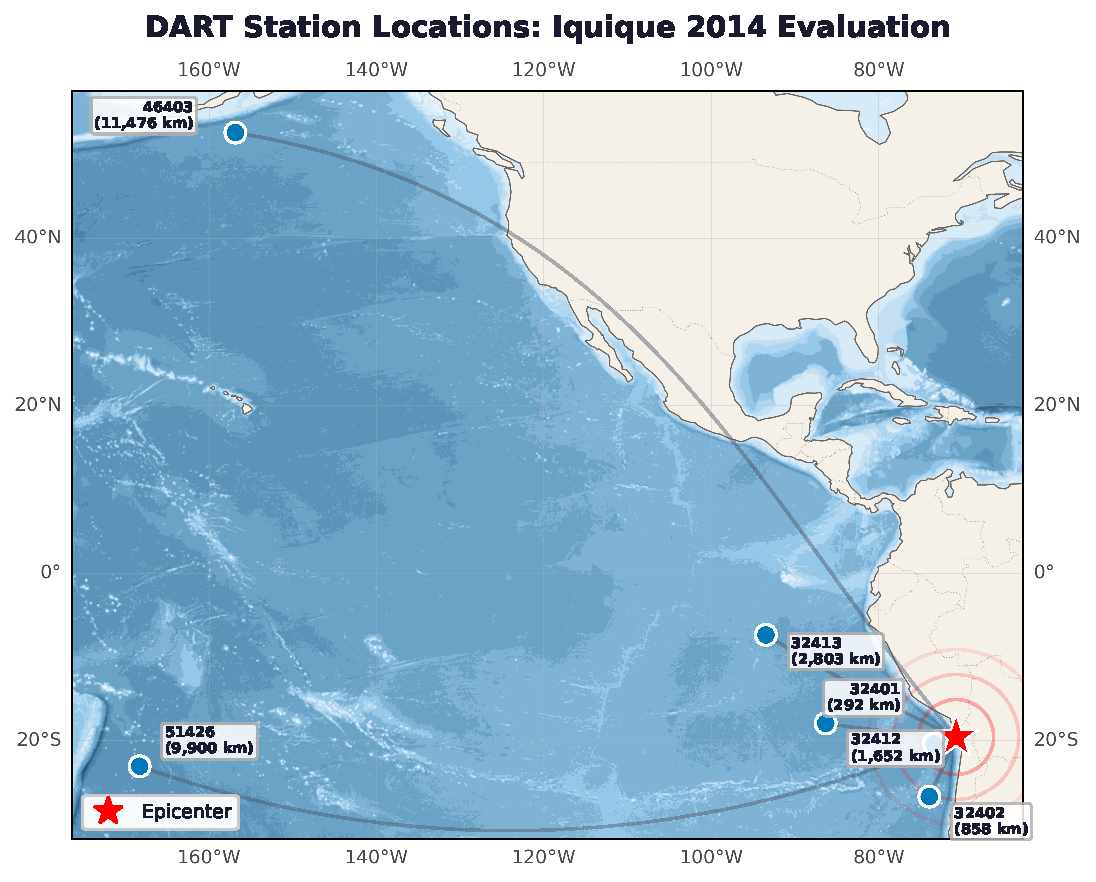
\includegraphics[width=\linewidth]{figures/fig_iquique_station_map.pdf}
  \caption{DART station locations; red star marks epicenter.}
  \label{fig:iquique-station-map}
\end{subfigure}
\caption{Iquique 2014 ($M_w$ 8.2) detection results and station geometry.
  (a) All four event-mode stations exceed INVESTIGATE; 32412 and 32413
  exceed ESCALATE. Standard-mode stations omitted
  (Table~\ref{tab:iquique-results}).
  (b) Epicenter at 19.610\textdegree S, 70.769\textdegree W.}
\end{figure}

\begin{figure}[!htbp]
\centering
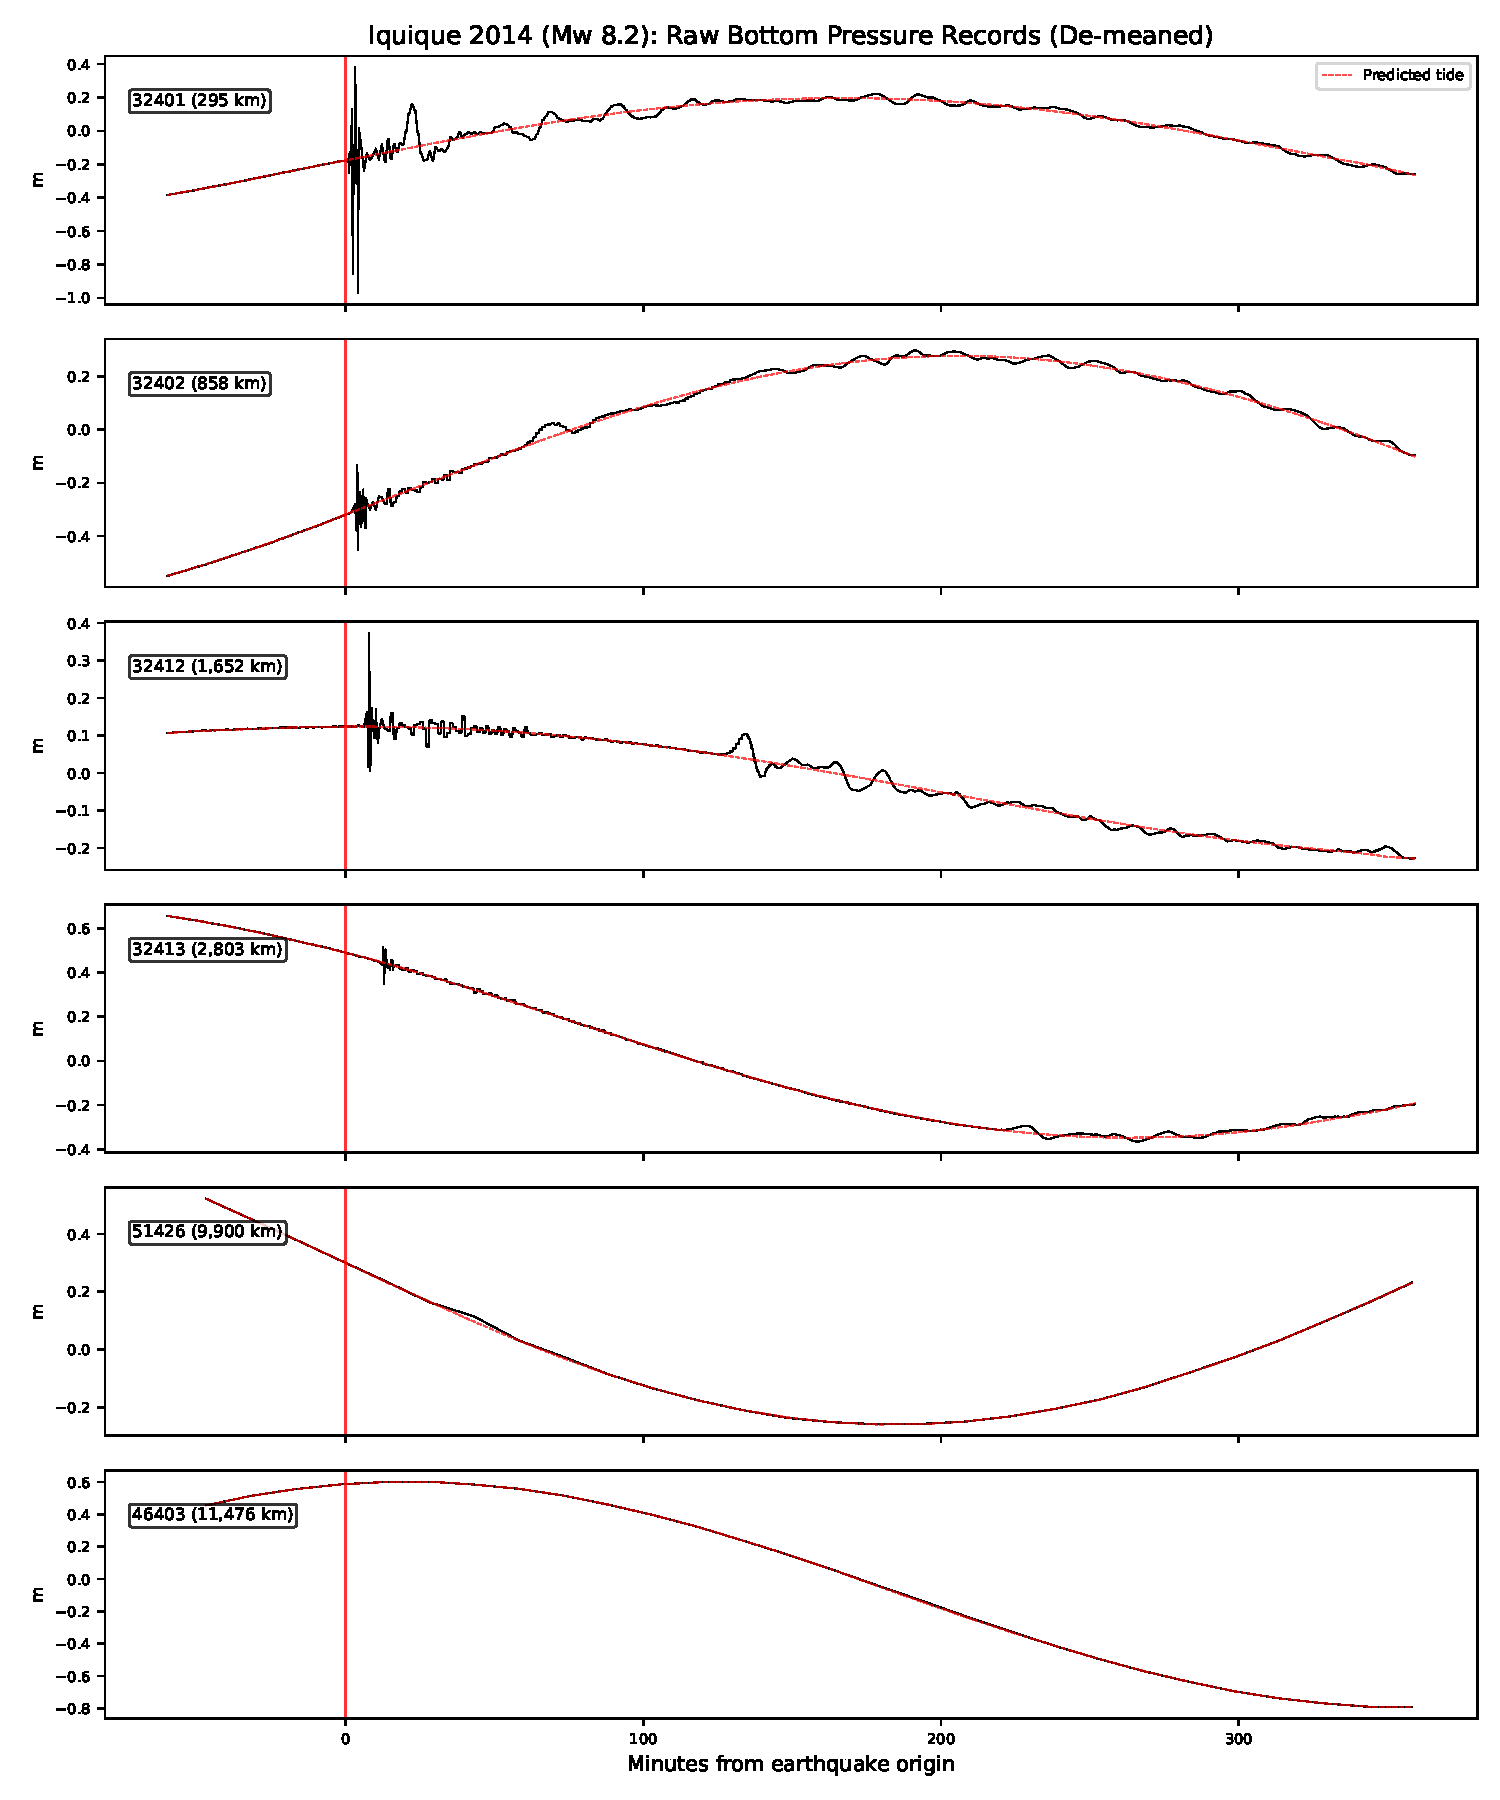
\includegraphics[width=0.92\linewidth]{figures/fig_iquique_waveforms.pdf}
\caption{Iquique 2014: raw bottom pressure records (de-meaned) for
  all six DART stations, ordered by epicentral distance.
  Red dashed: IRLS tidal prediction.
  Hatched regions indicate data gaps.}
\label{fig:iquique-waveforms}
\end{figure}

\begin{figure}[!htbp]
\centering
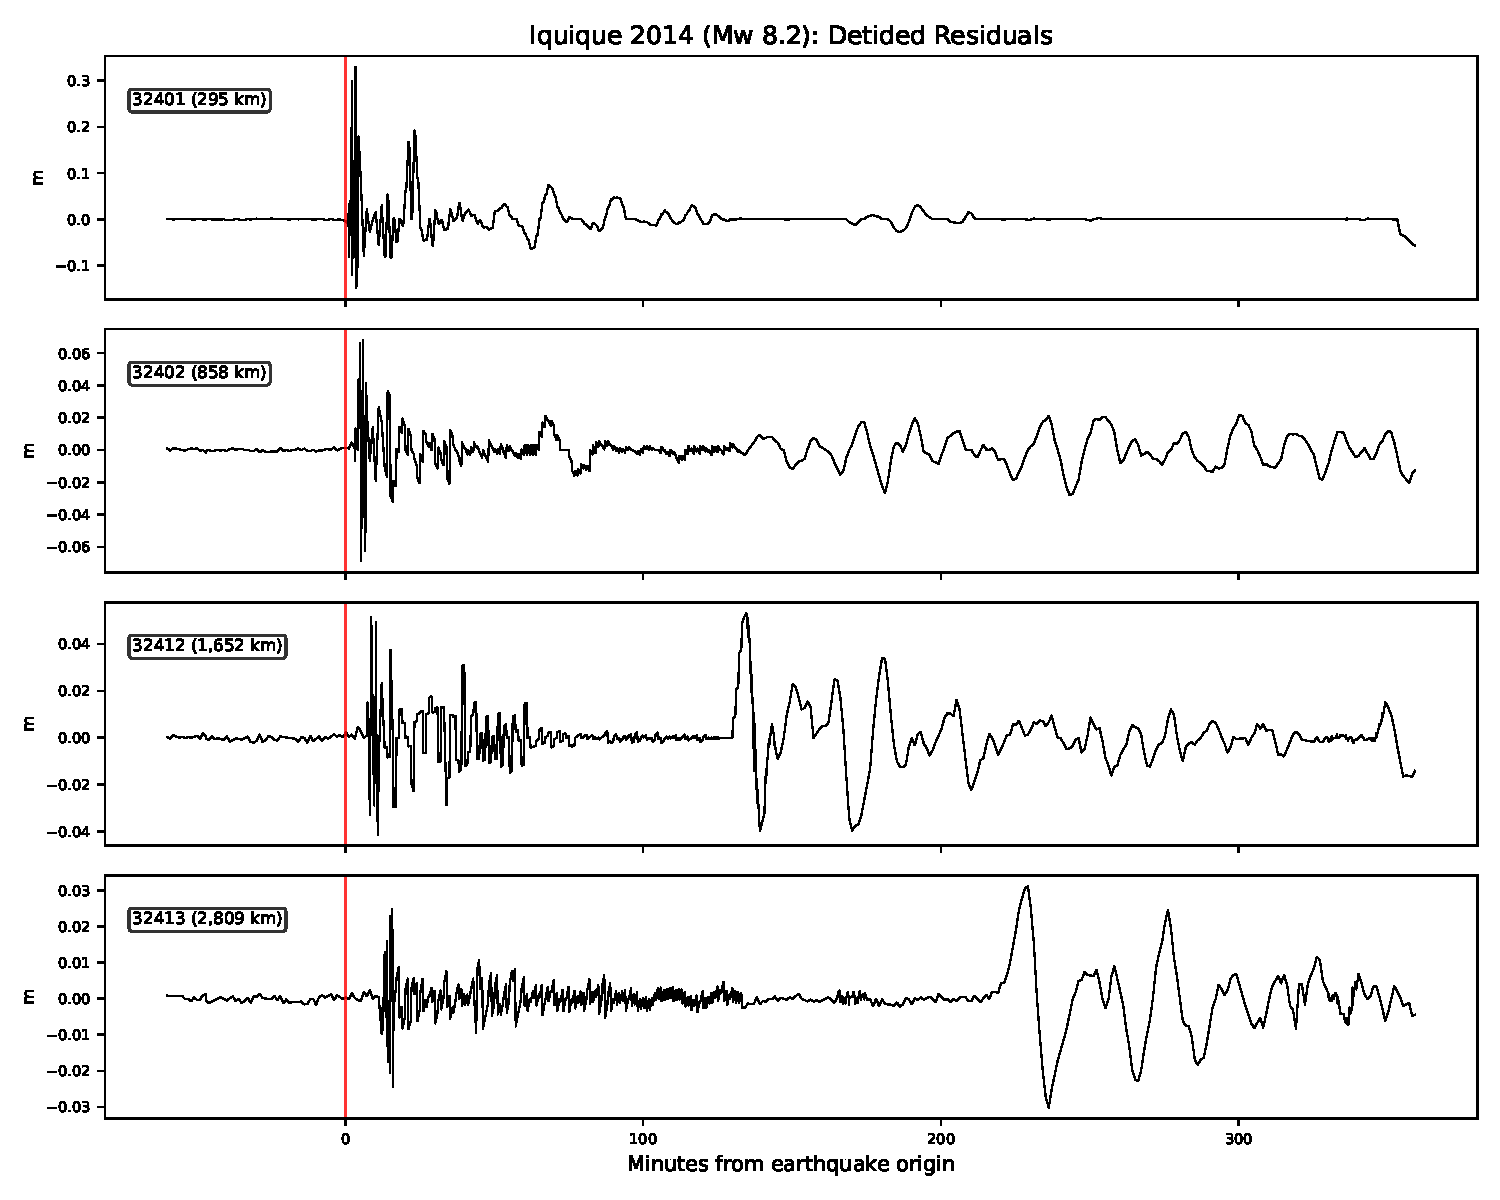
\includegraphics[width=0.92\linewidth]{figures/fig_iquique_residuals.pdf}
\caption{Iquique 2014: detided residuals for the four event-mode
  stations.  Despike, pre-event linear detrend, 30-min centered
  rolling median, and Hampel filter applied
  (Algorithm~\ref{alg:residual}).}
\label{fig:iquique-residuals}
\end{figure}

\begin{figure}[!htbp]
\centering
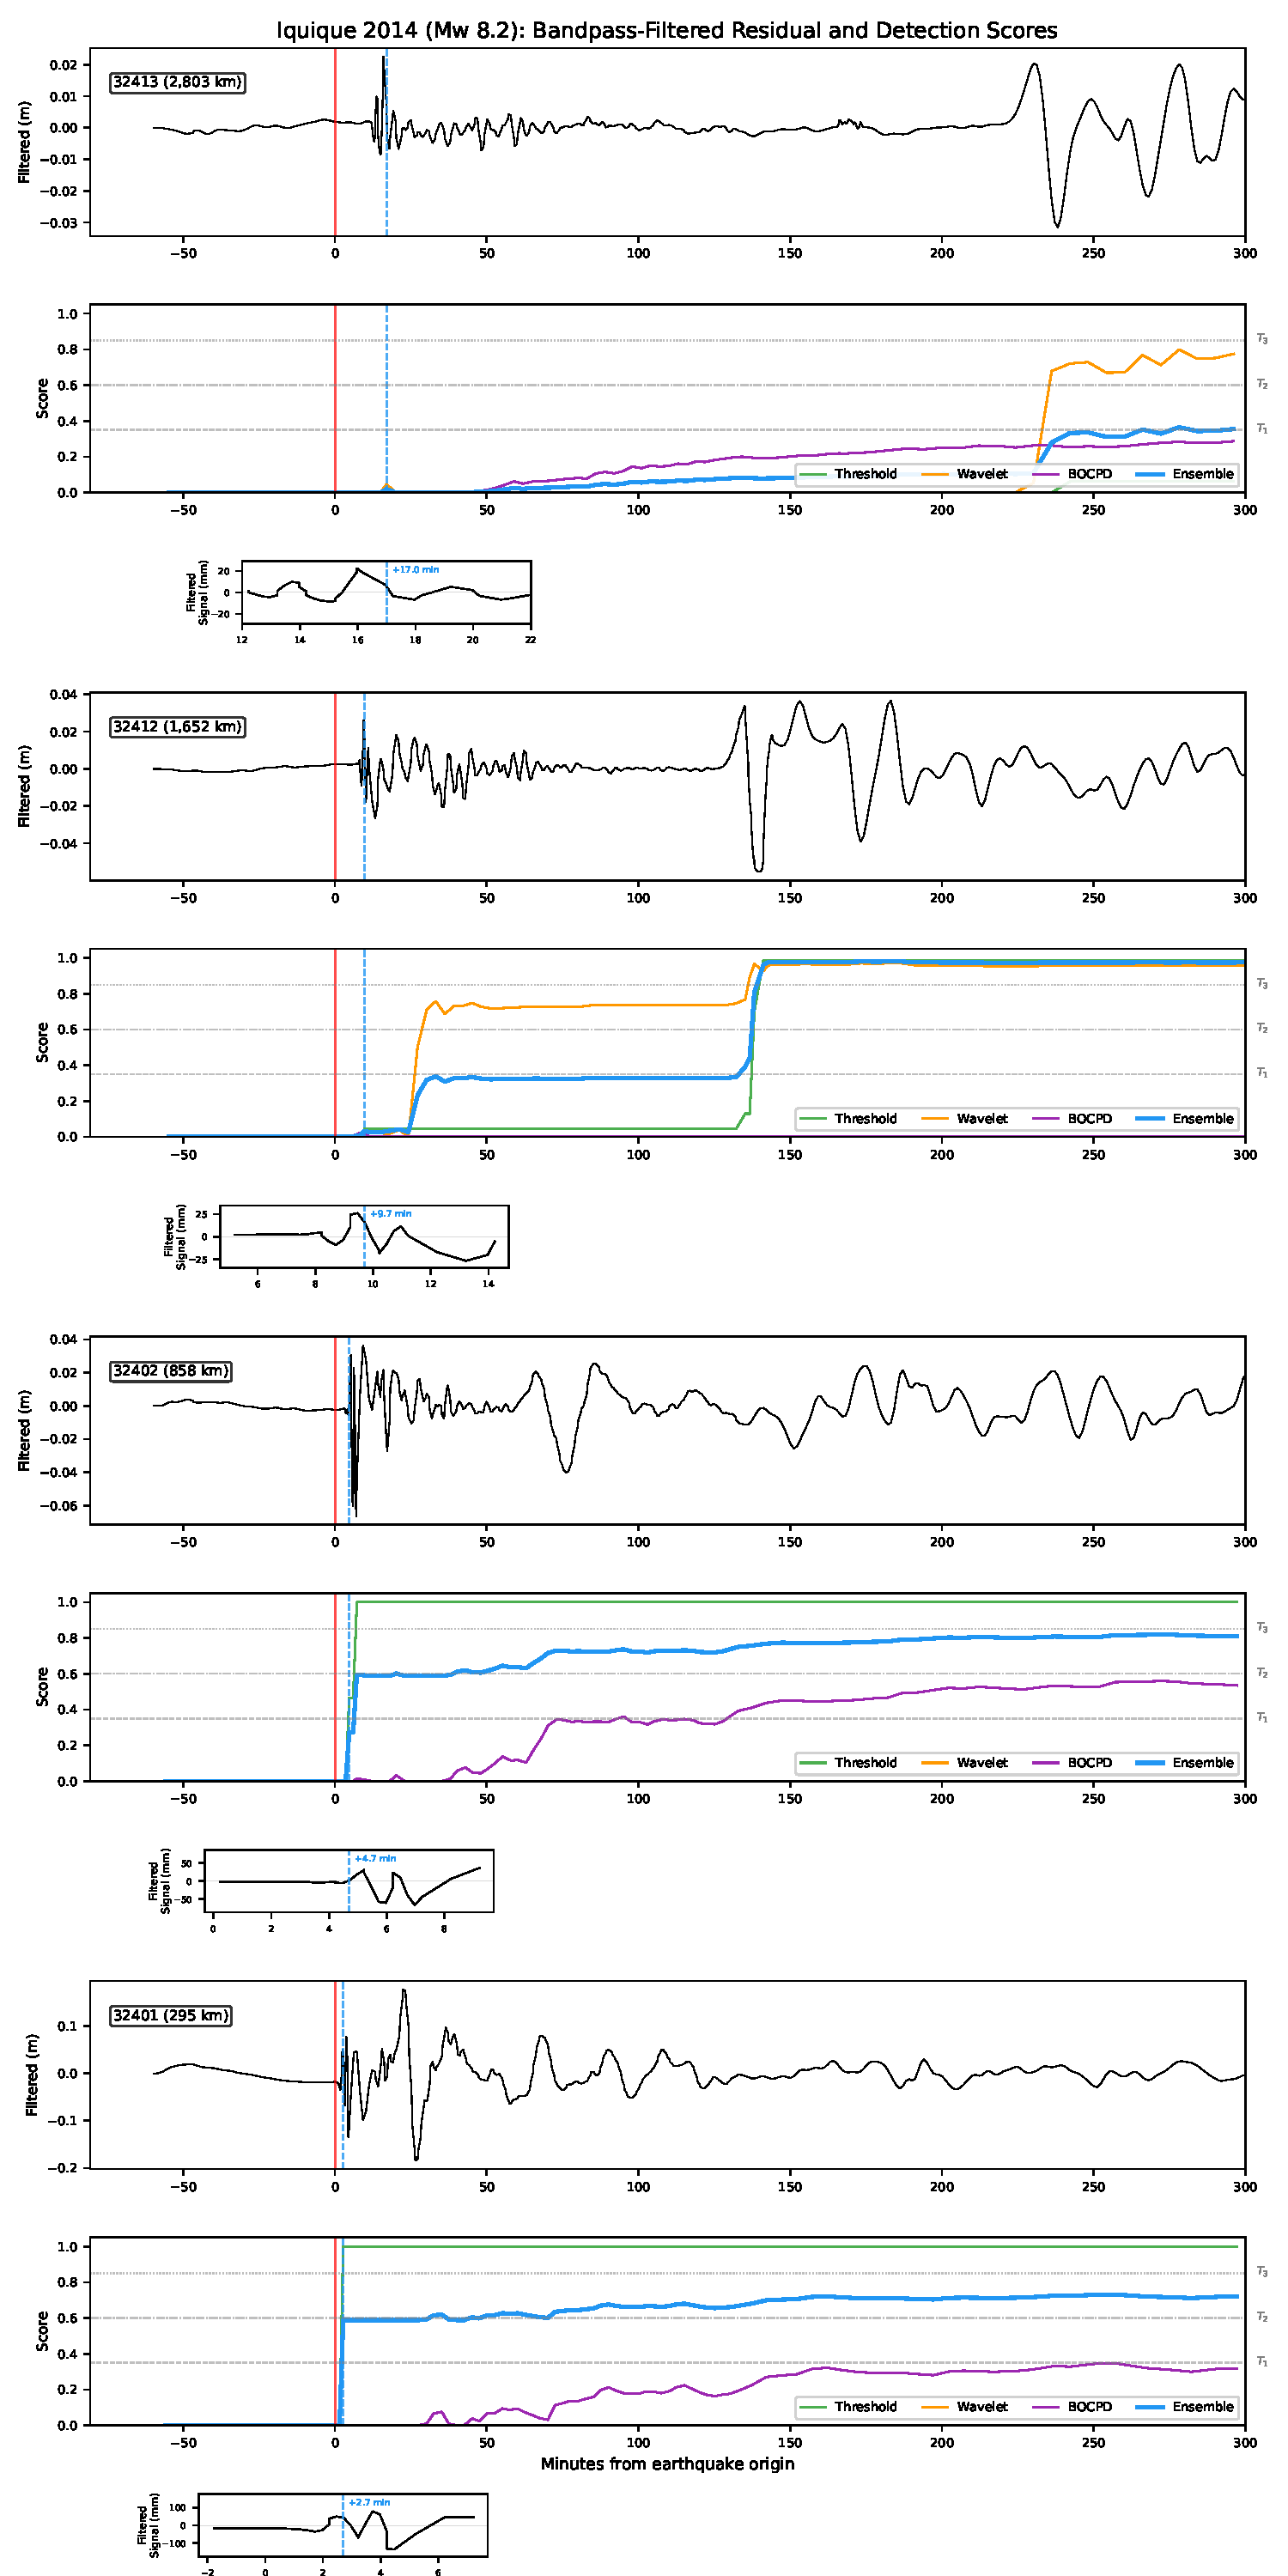
\includegraphics[width=\linewidth,height=0.85\textheight,keepaspectratio]{figures/fig_iquique_detection_timeline.pdf}
\caption{Detection pipeline signals and scores for Iquique 2014
  event-mode stations (matching Figure~\ref{fig:score-overlay} format).
  For each station: (top) bandpass-filtered detided residual
  (5--120\,min passband, causal Butterworth),
  (bottom) component and ensemble scores from sliding-window analysis
  with FSM thresholds $T_1$, $T_2$, $T_3$.
  Insets below each score panel show the signal at mm scale around
  score onset, the first nonzero ensemble score (blue dashed line).
  All four event-mode stations are shown.  Station 32413 (shortest calibration window of ${\sim}5.9$~days) achieves the highest
  ensemble score (1.000) despite the reduced baseline.}
\label{fig:iquique-timeline}
\end{figure}

\FloatBarrier
\subsection{Samoa 2009 Validation}
\label{sec:eval-samoa}

To test detection outside the Chile--Peru subduction zone,
we evaluate the 2009 Samoa $M_w$\,8.1 outer-rise earthquake
(2009-09-29 17:48:10 UTC; 15.489\textdegree S, 172.095\textdegree W;
depth 18\,km; USGS event usp000h1ys).
This event has an outer-rise normal-faulting mechanism,
distinct from the subduction-zone thrust events in the other four case
studies.  Seismologically, the 2009 Samoa--Tonga event was a triggered
doublet: the $M_w$\,8.1 outer-rise normal-faulting rupture triggered
near-simultaneous $M_w$\,8.0 thrust faulting on the Tonga
Trench~\citep{lay2010samoa}.  The DART records analyzed here contain
contributions from both sources; the pipeline's single-event FSM
processes the composite wavefield without source decomposition.
Six DART stations spanning 804--7{,}720\,km are selected
(Table~\ref{tab:samoa-stations}).

\begin{table}[!htb]
\centering
\caption{DART stations used in the Samoa 2009 retrospective validation
  (epicenter 15.489\textdegree{}S, 172.095\textdegree{}W).
  Distances computed via haversine.}
\label{tab:samoa-stations}
\small
\begin{tabular}{lrll}
\toprule
\textbf{Station} & \textbf{Dist.\,(km)} & \textbf{Location} & \textbf{Mode} \\
\midrule
51425 &    804  & NNE, near epicenter     & event (1\,min) \\
51426 &    935  & SSE, near Tonga         & event (1\,min) \\
54401 & 1{,}960 & S, south of Samoa       & event (1\,min) \\
51407 & 4{,}250 & NE, off Hawaii          & standard (15\,min) \\
46411 & 7{,}680 & NE, off N California    & standard (15\,min) \\
46403 & 7{,}720 & NE, off Alaska          & standard (15\,min) \\
\bottomrule
\end{tabular}
\end{table}

All three event-mode stations detect the event
(Figure~\ref{fig:samoa-detection}):
station 51426 (935\,km) achieves ensemble score 0.99 (ESCALATE),
54401 (1{,}960\,km) scores 0.76 (ASSESS), and
51425 (804\,km) scores 0.59 (INVESTIGATE).
Station 51425, despite being nearest, scores lowest among event-mode
stations because only the threshold detector fires (wavelet and BOCPD
both score zero), capping the ensemble at $0.588 \times 1.0 = 0.588$,
the single-detector maximum under the renormalized weighting.
The three far-field standard-mode stations show filter degradation.
Table~\ref{tab:samoa-results} provides the full per-station breakdown.
Raw pressure records with IRLS tidal fits are shown in
Figure~\ref{fig:samoa-waveforms}; detided residuals in
Figure~\ref{fig:samoa-residuals}; station geometry in
Figure~\ref{fig:samoa-station-map}; detection score timelines in
Figure~\ref{fig:samoa-timeline}.
CO-OPS water-level records, including the near-field Pago Pago
station, are shown in Appendix~\ref{sec:appendix-coops}
(Figure~\ref{fig:coops-samoa}).

\noindent\textbf{Agentic pipeline trace.}
The $M_w$\,8.1 outer-rise normal-faulting event at 18\,km depth
triggers seismic-only escalation.  DART evidence arrives at
+5.3\,min (stations 51425 and 51426 cross $T_1$ simultaneously).
Station 51426 reaches $T_3$ at +6.6\,min.
Station 51425 (804\,km) crosses $T_2$ at +17.8\,min in the
sliding timeline; over the full 6-hour window its ensemble is
0.588, with threshold as the sole contributing component
(wavelet and BOCPD both zero), demonstrating that the ensemble's
threshold-heavy renormalization preserves detection even when the
statistical component contributes nothing.
Audit trail:
(1)~\texttt{state\_transition}: IDLE~$\to$~MONITOR ($M$\,8.1);
(2)~\texttt{state\_transition}: MONITOR~$\to$~ESCALATE
(seismic-only, 18\,km);
(3)~\texttt{verification\_complete}: PASS\_WITH\_CONCERNS
(3 stations above $T_1$);
(4)~\texttt{report\_generated}: Tier~1, PROVISIONAL.

\begin{table}[!htb]
\centering
\caption{Samoa 2009 per-station anomaly detection results.
  Column definitions match Table~\ref{tab:tohoku-results}.}
\label{tab:samoa-results}
\footnotesize
\begin{tabular}{lrccccccccc}
\toprule
\textbf{Station} & \textbf{Dist (km)} & \textbf{Mode}
  & \textbf{Ens.} & \textbf{Thr.} & \textbf{Wav.}
  & \textbf{BCP} & \textbf{INV} & \textbf{ASS} & \textbf{ESC}
  & \textbf{Deg} \\
\midrule
51425 &    804    & event & 0.588 & 1.000 & 0.000 & 0.000 & \checkmark & ---        & ---        & --- \\
51426 &    935    & event & 0.986 & 1.000 & 0.966 & 0.000 & \checkmark & \checkmark & \checkmark & --- \\
54401 & 1{,}960   & event & 0.760 & 1.000 & 0.000 & 0.418 & \checkmark & \checkmark & ---        & --- \\
51407 & 4{,}250   & std   & 0.000 & 0.000 & 0.000 & 0.000 & ---        & ---        & ---        & \checkmark \\
46411 & 7{,}680   & std   & 0.000 & 0.000 & 0.000 & 0.000 & ---        & ---        & ---        & \checkmark \\
46403 & 7{,}720   & std   & 0.000 & 0.000 & 0.000 & 0.000 & ---        & ---        & ---        & \checkmark \\
\bottomrule
\end{tabular}
\end{table}

\begin{figure}[!htbp]
\centering
\begin{subfigure}[t]{0.52\linewidth}
  \centering
  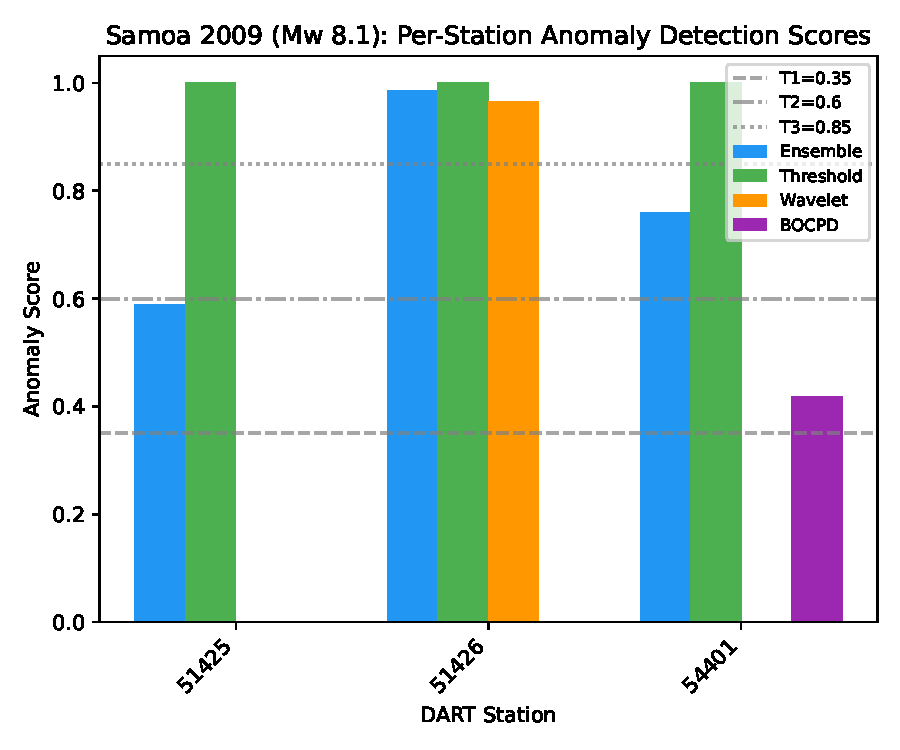
\includegraphics[width=\linewidth]{figures/fig_samoa_detection.pdf}
  \caption{Per-station anomaly scores (event-mode only).}
  \label{fig:samoa-detection}
\end{subfigure}\hfill
\begin{subfigure}[t]{0.46\linewidth}
  \centering
  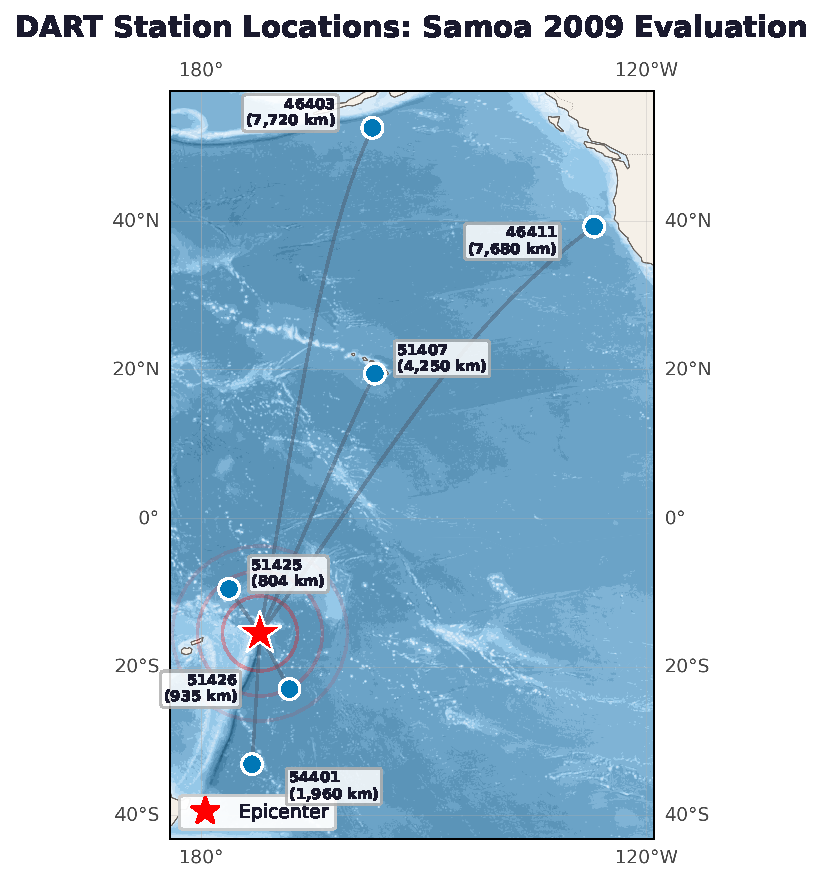
\includegraphics[width=\linewidth]{figures/fig_samoa_station_map.pdf}
  \caption{DART station locations; red star marks epicenter.}
  \label{fig:samoa-station-map}
\end{subfigure}
\caption{Samoa 2009 ($M_w$ 8.1) detection results and station geometry.
  (a) Three event-mode stations detect the event; 51426 exceeds ESCALATE.
  Standard-mode stations omitted (Table~\ref{tab:samoa-results}).
  (b) Epicenter at 15.489\textdegree S, 172.095\textdegree W.}
\end{figure}

\begin{figure}[!htbp]
\centering
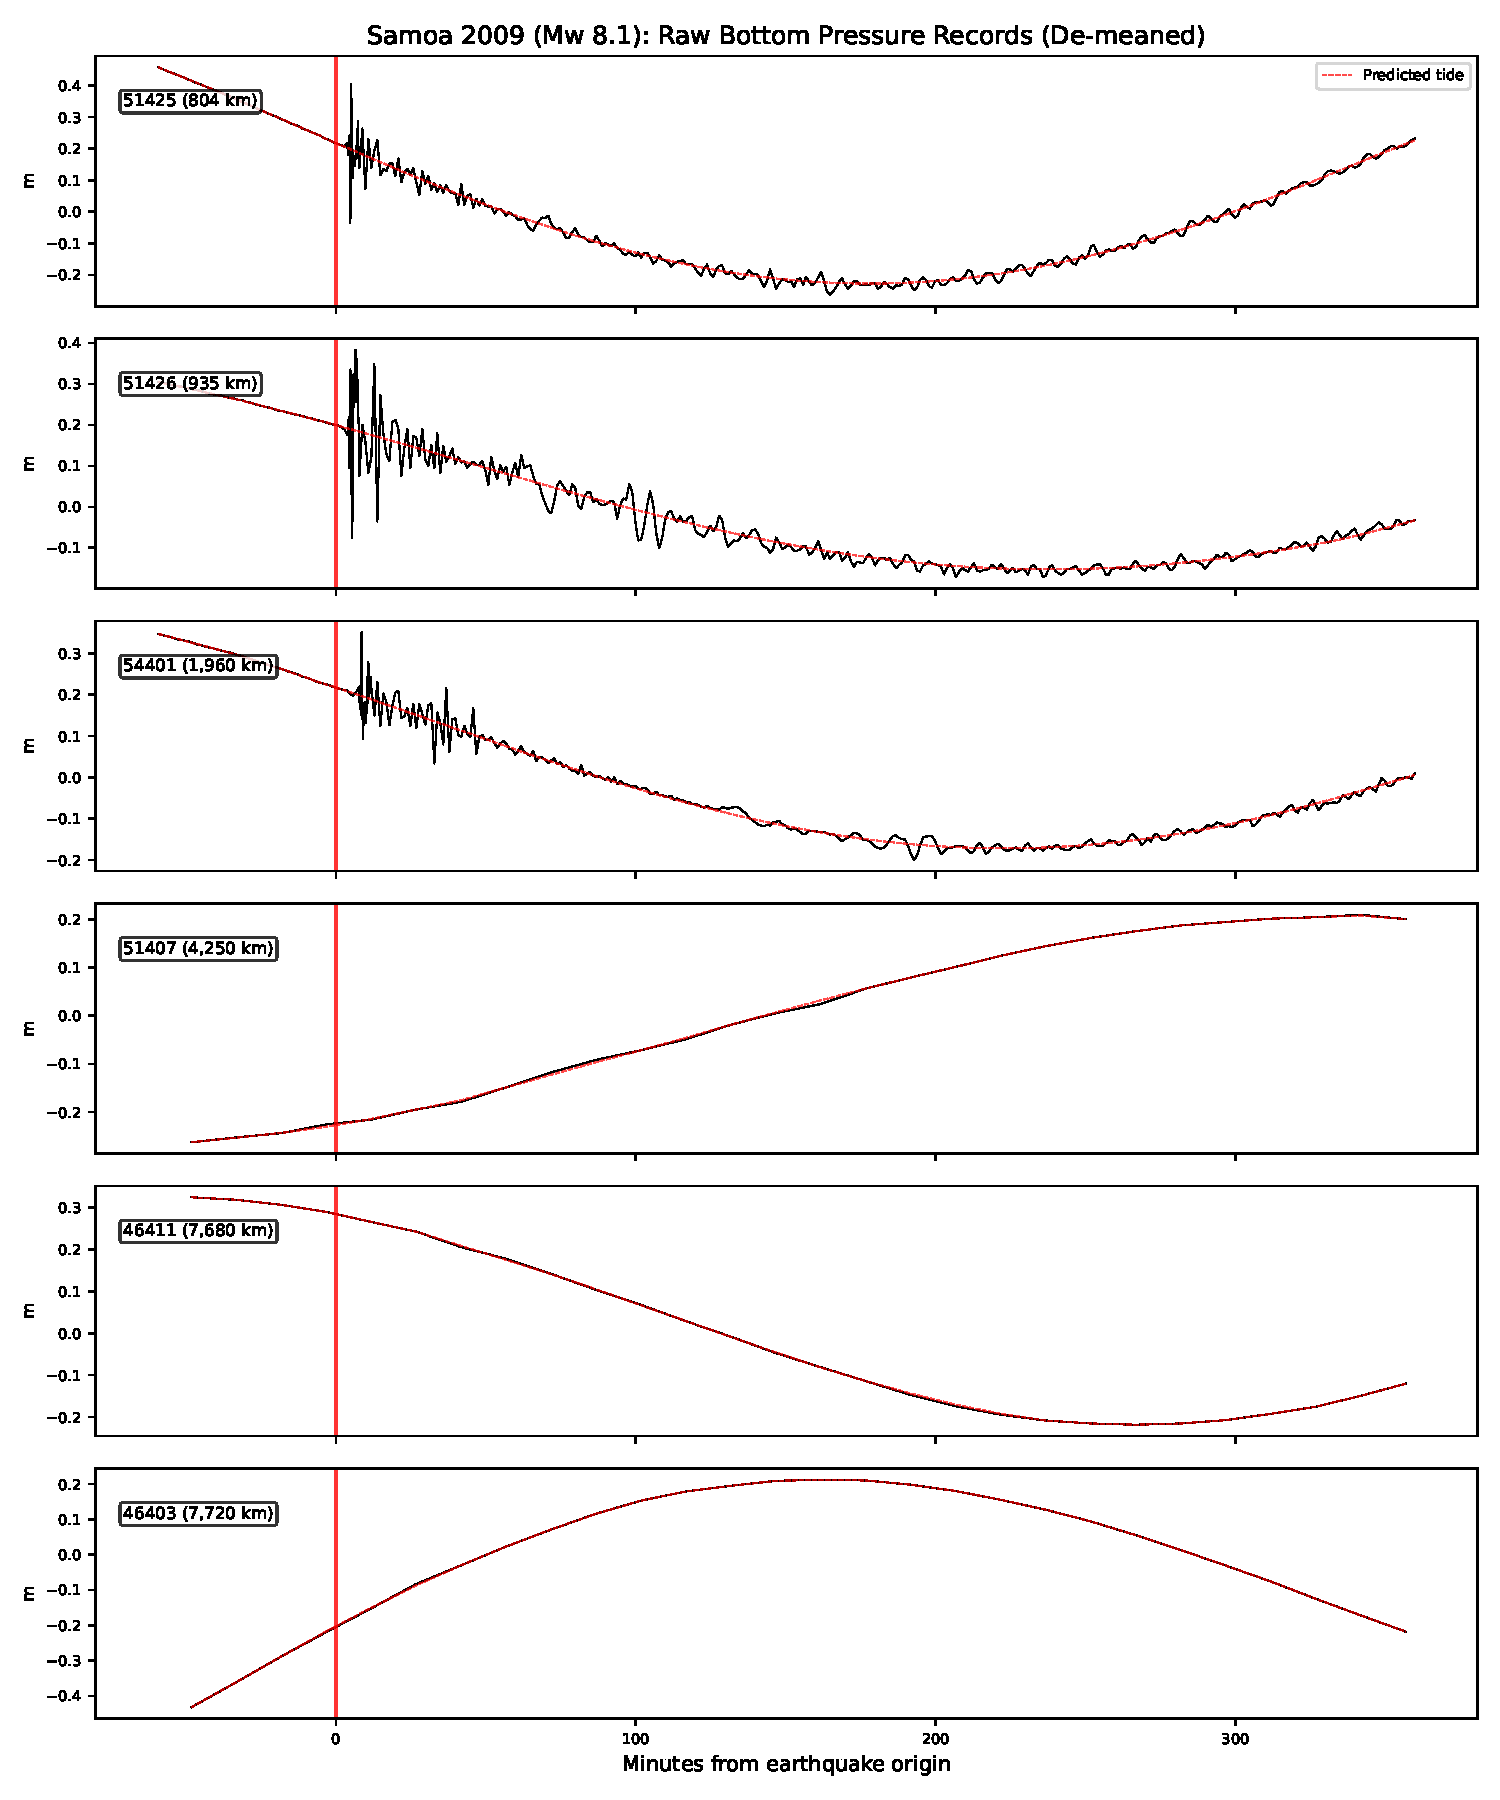
\includegraphics[width=0.92\linewidth]{figures/fig_samoa_waveforms.pdf}
\caption{Samoa 2009: raw bottom pressure records (de-meaned) for
  all six DART stations, ordered by epicentral distance.
  Red dashed: IRLS tidal prediction.
  Hatched regions indicate data gaps.}
\label{fig:samoa-waveforms}
\end{figure}

\begin{figure}[!htbp]
\centering
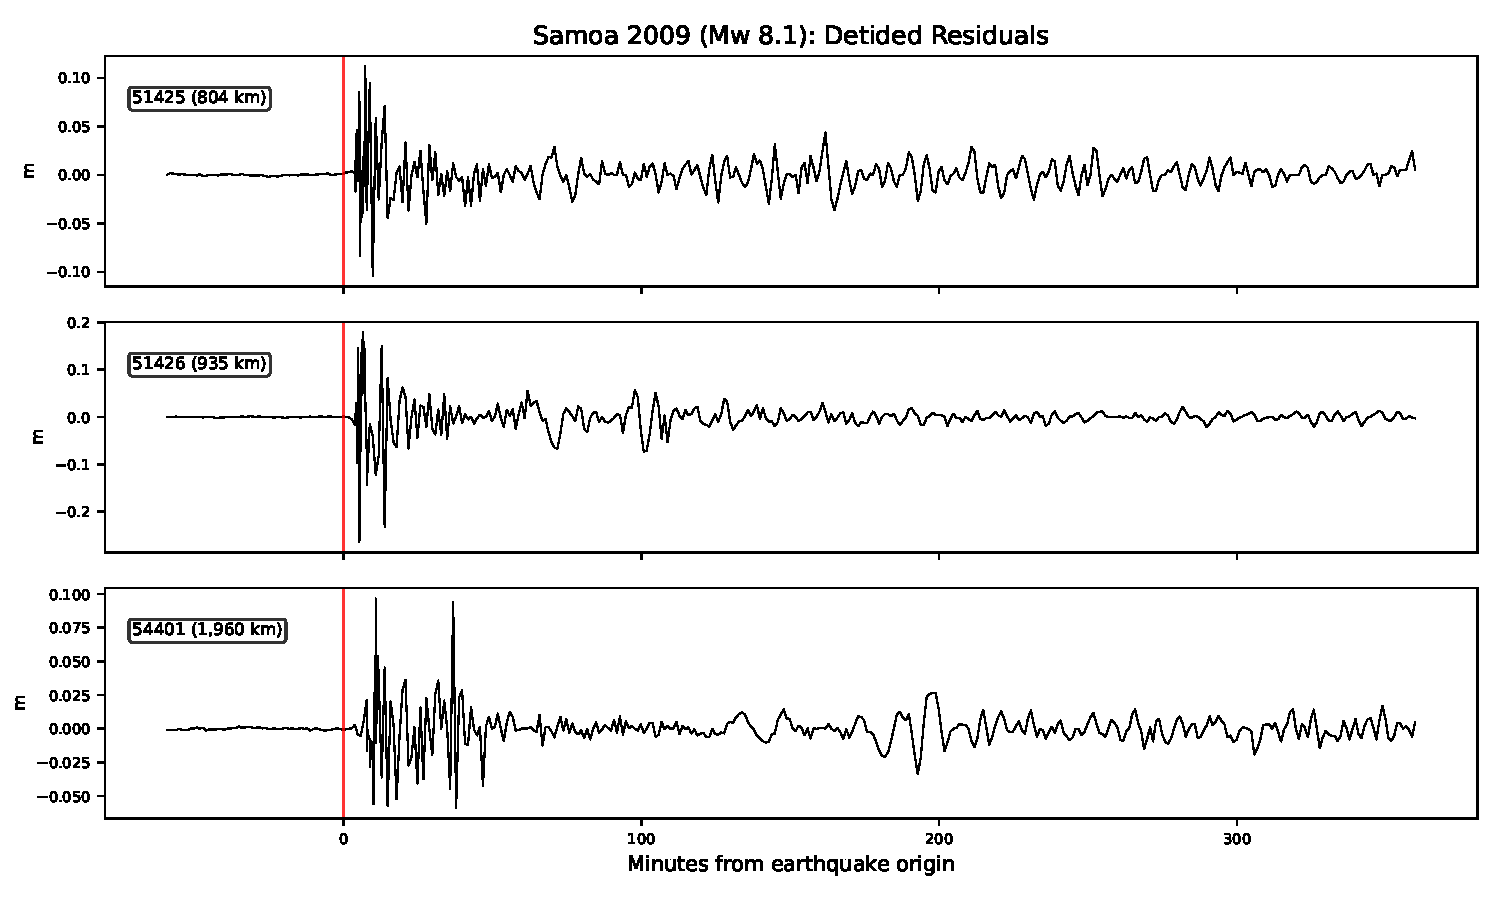
\includegraphics[width=0.92\linewidth]{figures/fig_samoa_residuals.pdf}
\caption{Samoa 2009: detided residuals for the three event-mode
  stations.  Despike, pre-event linear detrend, 30-min centered
  rolling median, and Hampel filter applied
  (Algorithm~\ref{alg:residual}).}
\label{fig:samoa-residuals}
\end{figure}

\begin{figure}[!htbp]
\centering
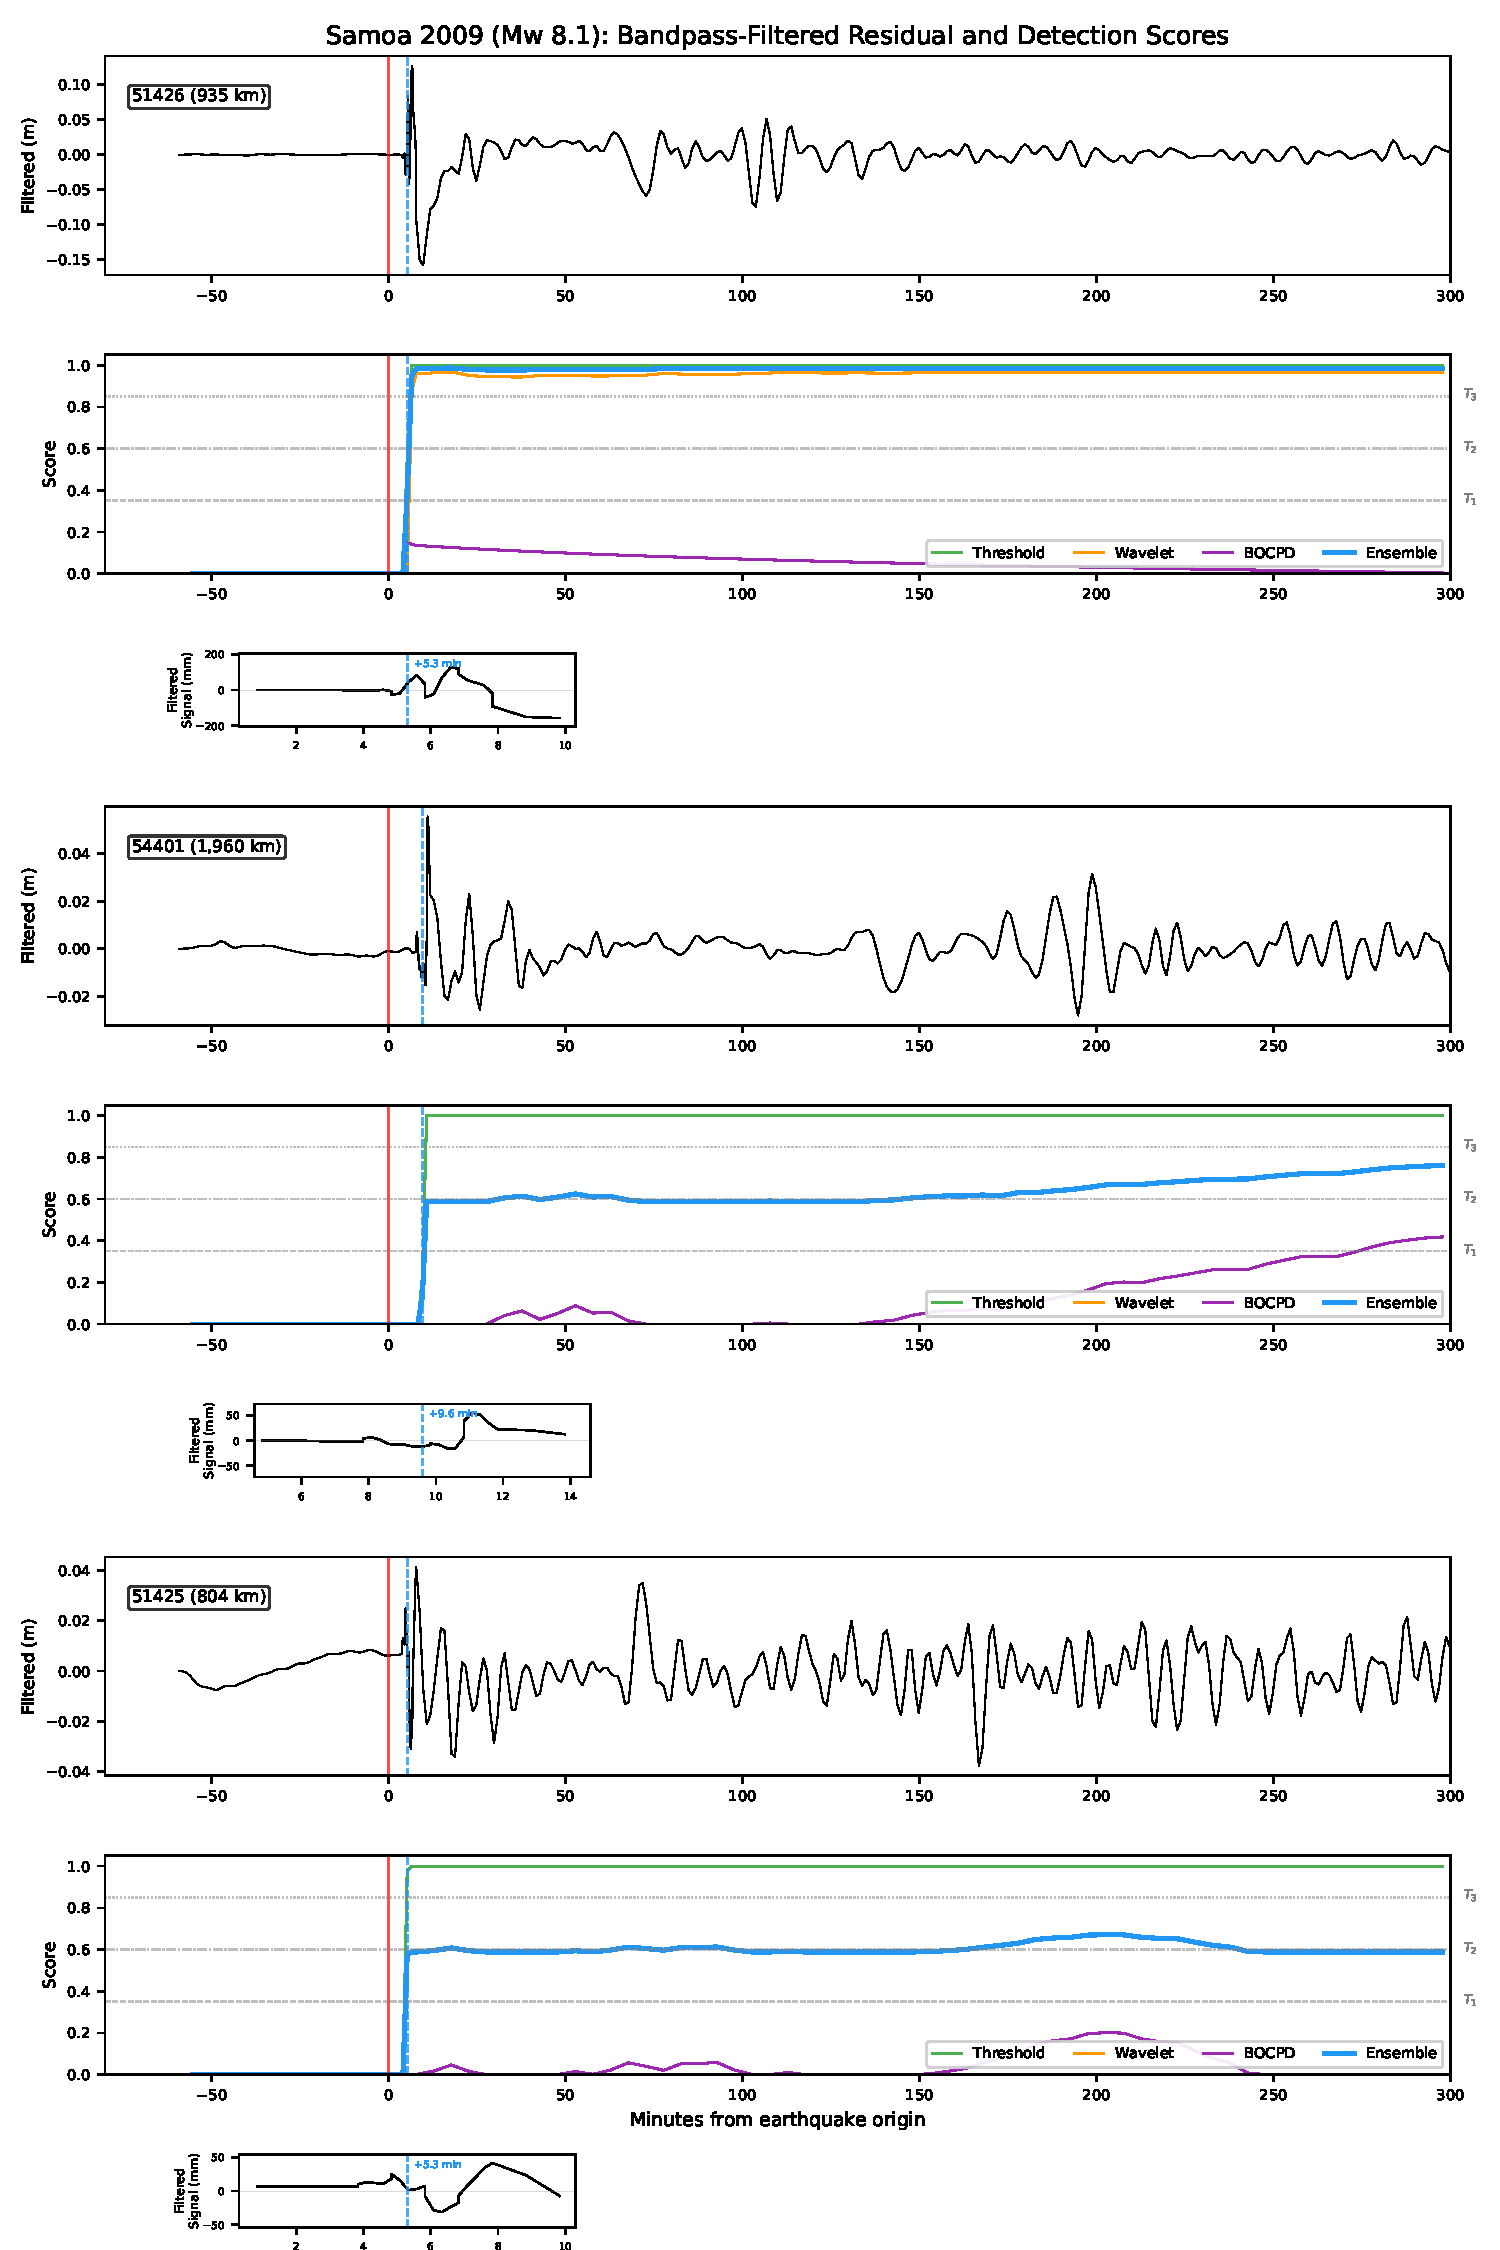
\includegraphics[width=\linewidth,height=0.85\textheight,keepaspectratio]{figures/fig_samoa_detection_timeline.pdf}
\caption{Detection pipeline signals and scores for Samoa 2009
  event-mode stations (matching Figure~\ref{fig:score-overlay} format).
  For each station: (top) bandpass-filtered detided residual
  (5--120\,min passband, causal Butterworth),
  (bottom) component and ensemble scores from sliding-window analysis
  with FSM thresholds $T_1$, $T_2$, $T_3$.
  Insets below each score panel show the signal at mm scale around
  score onset, the first nonzero ensemble score (blue dashed line).
  Station 51426 (935\,km) shows the strongest detection
  ($T_3$ crossing); station 54401 (1{,}960\,km) crosses $T_2$ with
  gradual BOCPD buildup; station 51425 (804\,km) crosses $T_2$ at
  +17.8\,min but not $T_3$.
  The outer-rise normal-faulting mechanism produces different
  waveform morphology compared to the thrust events.}
\label{fig:samoa-timeline}
\end{figure}


\end{document}
